%%%%%%%%%%%%%%%%%%%%%%%%%%%%%%%%%%%%%%%%%%%%%%%%%%%%%%%%%%%%%%%%%%% 
%                                                                 %
%                            ROOT FILE                            %
%                                                                 %
%%%%%%%%%%%%%%%%%%%%%%%%%%%%%%%%%%%%%%%%%%%%%%%%%%%%%%%%%%%%%%%%%%% 
%
%  Run LaTeX or pdfLaTeX on this file to produce your thesis.
%  To produce the abstract title page followed by the abstract,
%  see the file abstitle-phd.tex or abstitle-mas.tex.
%
%%%%%%%%%%%%%%%%%%%%%%%%%%%%%%%%%%%%%%%%%%%%%%%%%%%%%%%%%%%%%%%%%%%

\documentclass[chap]{thesis}

% Use the first command below if you want captions over 1 line indented. A side
% effect of this is to remove the use of bold for captions (thesis default).
% To restore bold, also include the second line below.



% \usepackage[hang]{caption}      % to indent subsequent lines of captions

\usepackage{graphics}
\usepackage{graphicx}
\usepackage{epstopdf}
\usepackage{epsfig}
\usepackage{url}
\urlstyle{rm}

% For algorithms
\usepackage{algorithmic}
\usepackage[chapter]{algorithm}

% For equations
\usepackage{amsmath}
\usepackage{amsfonts}
\usepackage{amssymb}

% For rotating in the tables
\usepackage{rotating} 
\usepackage[T1]{fontenc} 

% To make the text tighter
% \usepackage{microtype}


% % For hyperreffing
\usepackage{hyperref}
% \usepackage[backref]{hyperref}
\hypersetup{
    unicode=false,          % non-Latin characters in Acrobats bookmarks
    pdftoolbar=true,        % show Acrobats toolbar?
    pdfmenubar=true,        % show Acrobats menu?
    pdffitwindow=true,      % page fit to window when opened
    pdftitle={My title},    % title
    pdfauthor={Author},     % author
    pdfsubject={Subject},   % subject of the document
    pdfnewwindow=true,      % links in new window
    pdfkeywords={keywords}, % list of keywords
    colorlinks=true,       % false: boxed links; true: colored links
    linkcolor=black,          % color of internal links
    citecolor=black,        % color of links to bibliography
    filecolor=black,      % color of file links
    urlcolor=black          % zcolor of external links
}


% \usepackage[american]{babel}
% \usepackage{csquotes}
% \usepackage{biblatex}
% \bibliography{Thesis}

%  \renewcommand{\captionfont}{\bfseries} % bold caption (needed with caption 
                                       % package to restore boldface.)
% \includeonly{1-Introduction, 2-PriorArt}  % use \includeonly to process only
                         % the file(s) listed inside the braces                       
\begin{document}

% Supply information for title page (copied from rpititle-phd.tex):    
\thesistitle{\bf Representation and Generation of Terrain Using Mathematical Modeling}        
\author{Christopher S. Stuetzle}        
\degree{Doctor of Philosophy}        
\department{Computer Science} % provide your area of study here; e.g.,
\signaturelines{4}     % max number of signature lines is 7        
\thadviser{W. Randolph Franklin}
\cothadviser{Barbara Cutler} % If you have 2 thesis advisers
\memberone{Thomas Zimmie}        
\membertwo{Petros Drineas}        
\submitdate{June 2012\\(For Graduation December 2012)} 
\copyrightyear{2012}   % if omitted, current year is used.        

% Print titlepage and other prefatory material:
%    
\titlepage     
\copyrightpage         % optional           
\tableofcontents        
\listoftables          % required if there are tables
\listoffigures         % required if there are figures
\listofalgorithms      % list of algorithms   % titlepage material for PhD thesis 
%%%%%%%%%%%%%%%%%%%%%%%%%%%%%%%%%%%%%%%%%%%%%%%%%%%%%%%%%%%%%%%%%%% 
%                                                                 %
%                         ACKNOWLEDGEMENT                         %
%                                                                 %
%%%%%%%%%%%%%%%%%%%%%%%%%%%%%%%%%%%%%%%%%%%%%%%%%%%%%%%%%%%%%%%%%%% 
 
\specialhead{ACKNOWLEDGMENT}
 
I would like to thank my advisers, W. Randolph Franklin and Barb Cutler, for their seemingly endless patience and encouragement. I would like to thank my family and friends, without whose faith in me this would not have been possible. I would like to thank my committee members for the generous commitment of their time, and the rest of the RPI community for providing me with every possible opportunity to succeed.
% 
This research was partially supported by NSF grants CMMI-0835762 and IIS-1117277.
%%%%%%%%%%%%%%%%%%%%%%%%%%%%%%%%%%%%%%%%%%%%%%%%%%%%%%%%%%%%%%%%%%% 
%                                                                 %
%                            ABSTRACT                             %
%                                                                 %
%%%%%%%%%%%%%%%%%%%%%%%%%%%%%%%%%%%%%%%%%%%%%%%%%%%%%%%%%%%%%%%%%%% 
 
\specialhead{ABSTRACT}
 
% \fbox{Will write abstract}

This thesis presents a detailed look at terrain modeling through the lens of mathematical analysis, and explores representation of the terrain surface 
through mathematical operations, descriptive statistics, and erosion simulation.
Modeling terrain surfaces is an essential aspect in a variety of applications in Geographic Information Science, from path planning to dam siting to terrain compression and beyond.
This work presents a novel representation of terrain that maintains its shape properties while facilitating the representation of hydrographically valid terrains, capturing the richness of the physics of the terrain's generation by digging channels in the surface.
% The accuracy of this representation is tested with a series of terrain distance metrics, including an adaptation of the Hausdorff distance.
Terrains are also described by a series of statistical characteristics known as the terrain fingerprint. These characteristics describe the behavior of water flow on the surface, and in turn can be used to compare terrain datasets.
This work also presents a simulation of hydraulic erosion on earthen embankments, motivated by the catastrophe in New Orleans during Hurricane Katrina. The generation of terrain data through erosion simulation is a well-studied problem, but the goal of the simulation in this work is the accuracy of the formation, and as such it is validated with laboratory experiments.
Finally, this thesis presents an application for exploring and manipulating terrain data in a group collaboration environment through the use of a novel multi-user laser tracking and identification system.
% This work explores the mathematics of terrain data through representation, generation, and statistical description.


\chapter {The Mathematics of Terrain}
\label{chapter:Introduction}

The surface of the Earth is one of the largest and most influential sources of data there is. 
Its shape determines atmospheric conditions, where structures can and should be built, and where flooding is to be expected, for example. 
As such, our quest for full understanding of the physical environment around us relies on an understanding of the underlying mathematics of the Earth's surface.
Therefore terrain data, both surface and volumetric, are vital for a wide array of applications in Computer Graphics and Geographic Information Science (GIS).

% GIS is the discipline charged with collecting, analyzing, and manipulating terrain data. One of the primary challenges in GIS is understanding the underlying mathematics of terrain, and using that understanding to develop more accurate and robust representations of the data that take into account the terrain's hydrography, or behavior of water on the terrain.
% 
This thesis presents a detailed look at terrain modeling through the lens of mathematical analysis, and explores representation and generation of the terrain surface 
through mathematical operations, descriptive statistics, and erosion simulation.




% It presents a method for modeling and representing terrain that is more closely related to the physics of erosion than previous methods based on mathematical operations that
% % , when combined with each other and various parameters, 
% procedurally generate the terrain based on the physical impact of erosion on a terrain surface.
% % , and their mathematical properties are be explored in depth. 
% This model allows for better compression of terrain datasets, as well as a terrain shape that more closely resembles reality than other popular models.
% This work also presents a series of metrics for determining statistical distance between two terrains, including the idea of a terrain "fingerprint", which is a measurement of a series of characteristics based on the terrain's hydrography data.
% %  used to better determine similarity and dissimilarity between terrains and channel networks extracted from those terrains. 
% % These fingerprints lead directly to a method of terrain comparison which determines a "distance" between two terrains, and is used to critically examine the erosion processes that alter the terrain. 
% % Data is collected through the use of a visually-validated and physically based erosion simulation based on smoothed particle hydrodynamics and a model of soil erodibility. This data is processed and allows me to capture snapshots of terrain evolution.
% In addition to modeling the surface with mathematical operations, this thesis presents the work of a research group that has investigated the process of erosion on levee surfaces, and validates the group's results through comparison to laboratory experimentation. 

\section{Modeling Terrain Surfaces}
\label{section:ModelingTerrainSurfaces}

Geographic Information Science is the study, manipulation, collection, management, and analysis of all geographical information, 
blending cartography, modeling, and data analysis and statistics.
One of the primary challenges in GIS is understanding the underlying mathematics of terrain surface data in order to model it accurately, robustly, and compactly.

Between the fields of earth science, computer science, mathematics, physics, and civil engineering, a good deal of work has revolved around modeling terrain surfaces. It is an essential aspect in a variety of applications in GIS, from path planning to dam siting to terrain compression. However, despite the large body of excellent work from which to draw, GIS still lacks a physically realistic representation of terrain that stems from a 
% deep
mathematical understanding of the way in which erosion processes, most specifically hydraulic erosion (the wearing away of a material due to water), contribute to the evolution and formation of a terrain. 
In addition to simply providing for more accurate data, an accurate and compact terrain representation lends itself naturally to better compression schemes, faster algorithms, and more accurate terrain generation. 


The hydrography, or behavior of water, of the terrain is a fundamental property that influences many of the characteristics of the terrain,
% Many applications in GIS (including those presented in this thesis) rely on the hydrography of the terrain, which is represented 
and it governs many of the applications in GIS. 
It is defined by the direction of water flow across the terrain, and allows for the extraction of the channel network (also know as the river or drainage network) of the terrain surface, 
a series of channel segments that join and flow together toward a sink.
Maintaining this critical information should be a primary objective of any terrain representation or generation scheme,
as important applications (such as modeling erosion on earthen embankments, as discussed in Sections \ref{section:ModelingLeveeFailure} and \ref{chapter:ErosionSimulation}) require hydrographically sound terrain representations.


With these goals in mind, this work focuses on the representation and generation of valid terrain, or data that 
% more 
closely mimics real life terrain. Real terrain is not a continuous surface, as discontinuities are common. Cliff faces, the sides of rivers, and caves are all terrain features that introduce discontinuities to any terrain surface representation. 
% Also, local minima (pits, for instance) are hard to find in real terrain, and are often introduced in data as a consequence of inaccuracies in data collection. 
In addition, local minima, or pits, are known to exist in certain terrains, such as those consisting of Karst topography or natural basins (e.g. endorheic basins). 
% \fbox{CITATIONS FOR THEM?}
However, most
local minima present in terrain data are a result of the sampling procedure used to collect it, which may miss channels
that are too small for the spacing of the grid and may
pass between sample points (sometimes called ``posts''). 
Most data collection techniques cannot differentiate between tree cover, lake surfaces, and land, resulting in elevation inaccuracies and pits where there should be none.
% At the scale at which most of these data are collected (with approximately 30 m spacing), local minima should not appear as often as they do. 
One of the principal constraints of any new representation is that it must facilitate the restriction of local minima, especially along the terrain's drainage network, by drawing a connection between the representation and the physics of the terrain's formation.

A method for modeling and representing terrain based on a mathematical operator, the \emph{drill operator}, is presented. This representation is more closely related to the physics of erosion than other purely spatial representations. It also facilitates enforcement of rules to limit the presence of local minima, and allows for discontinuities in the surface to be encoded. 
% than previous methods
 With various parameters, terrain is procedurally and accurately generated. This operator is based on the physical impact of erosion on a terrain surface, and its mathematical properties are explored in depth. 
This model allows for better data compression of terrains, as well as a terrain shape that more closely resembles reality than other popular models.

Current terrain representations are generally variations of either height fields (2D pixel grids of elevations, also known as Digital Elevation Models, or DEMs) or piecewise linear triangular splines (also known as Triangulated Irregular Networks, or TINs). Both of these representations have advantages and disadvantages, but neither sufficiently captures the physical complexity of a terrain surface. For instance, neither can accurately handle discontinuities on the surface, such as cliff faces. 
Each representation is single-valued, meaning that each vertex of data has a unique x,y coordinate. Since the slope of a cliff face is vertical, and as such undefined, any single-valued representation cannot accurately model it.
% 
% TINs are able to, but with added complexity to any algorithm using them, since many applications rely on the grid regularity of the TIN representation. 
Volumetric representations, such as voxel grids, allow for said discontinuities as well as volumetric features such as caves, but have considerable memory footprints, and do not correlate in any way with the geological processes that formed the terrain being represented. 

% \fbox{WTF?}
% A set of procedural steps utilizing a finite set of well-defined drill operators that mimic erosion to form a terrain both saves space and allows for more physically accurate surface features, such as discontinuities and a lack of local minima.

To facilitate the development and testing of the drill operator, a more fundamental understanding of the 
% statistics and characteristics of terrains is necessary. 
% What are the characteristics of terrain necessary to mimic? 
% What are the characteristics of terrain necessary to maintain when compressing it? 
% Part of the answer to these questions lies in the hydrography of the terrain. 
% 
effects and behavior of water on the surface, also known as the terrain's hydrography, is necessary.
This fundamental characteristic can be described by the terrain's channel network, or a series of pixels that describe the flow of water across the surface.
% 
Several methods exist for extracting the channel network,
%(see section \ref{section:PriorLiteratureChannelNetworkExtraction}), 
and much can be done with the information gleaned from it.  
Terrain statistics such as 
% the channel width and depth, 
how much network segments meander, the relative importance of pixels within the network, and the balance of tributaries that join major rivers are measured.
This statistical approach provides a descriptive picture of a terrain that is useful when comparing two terrains (for applications such as measuring compression scheme accuracy), as well as describing the erosion processes responsible for the formation of the terrain.
% Also presented 
This is the \emph{terrain fingerprint}, a series of terrain characteristics used to better determine similarity and dissimilarity between terrains and channel networks extracted from those terrains. These fingerprints lead directly to a method of terrain comparison which determines a metric of distance between two terrains.
% , and is used to critically examine the erosion processes that alter the terrain. 



\begin{figure}[t]
  \centering
  \begin{minipage}{0.99\textwidth}
    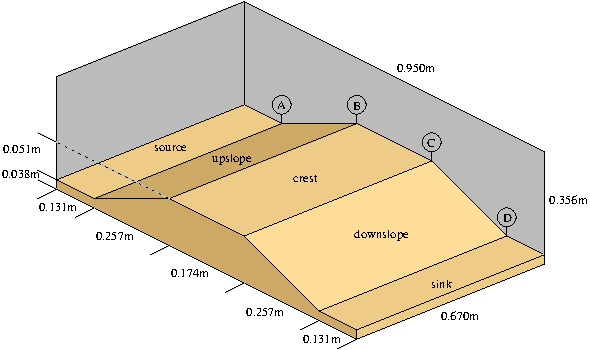
\includegraphics[width=1.0\textwidth]{images/levee_diagram.pdf}
  \end{minipage}
  \caption[Annotated diagram of a levee]{An annotated diagram of a levee, detailing the wet side (source, upslope), crest, and dry side (downslope, sink). Measurements refer to those of model levees created in a laboratory for experimentation.}
  \label{figure:levee_diagram}
\end{figure}



\section{Modeling Levee Failure}
\label{section:ModelingLeveeFailure}

\begin{figure}[t]
  \centering
  \begin{minipage}{0.49\textwidth}
    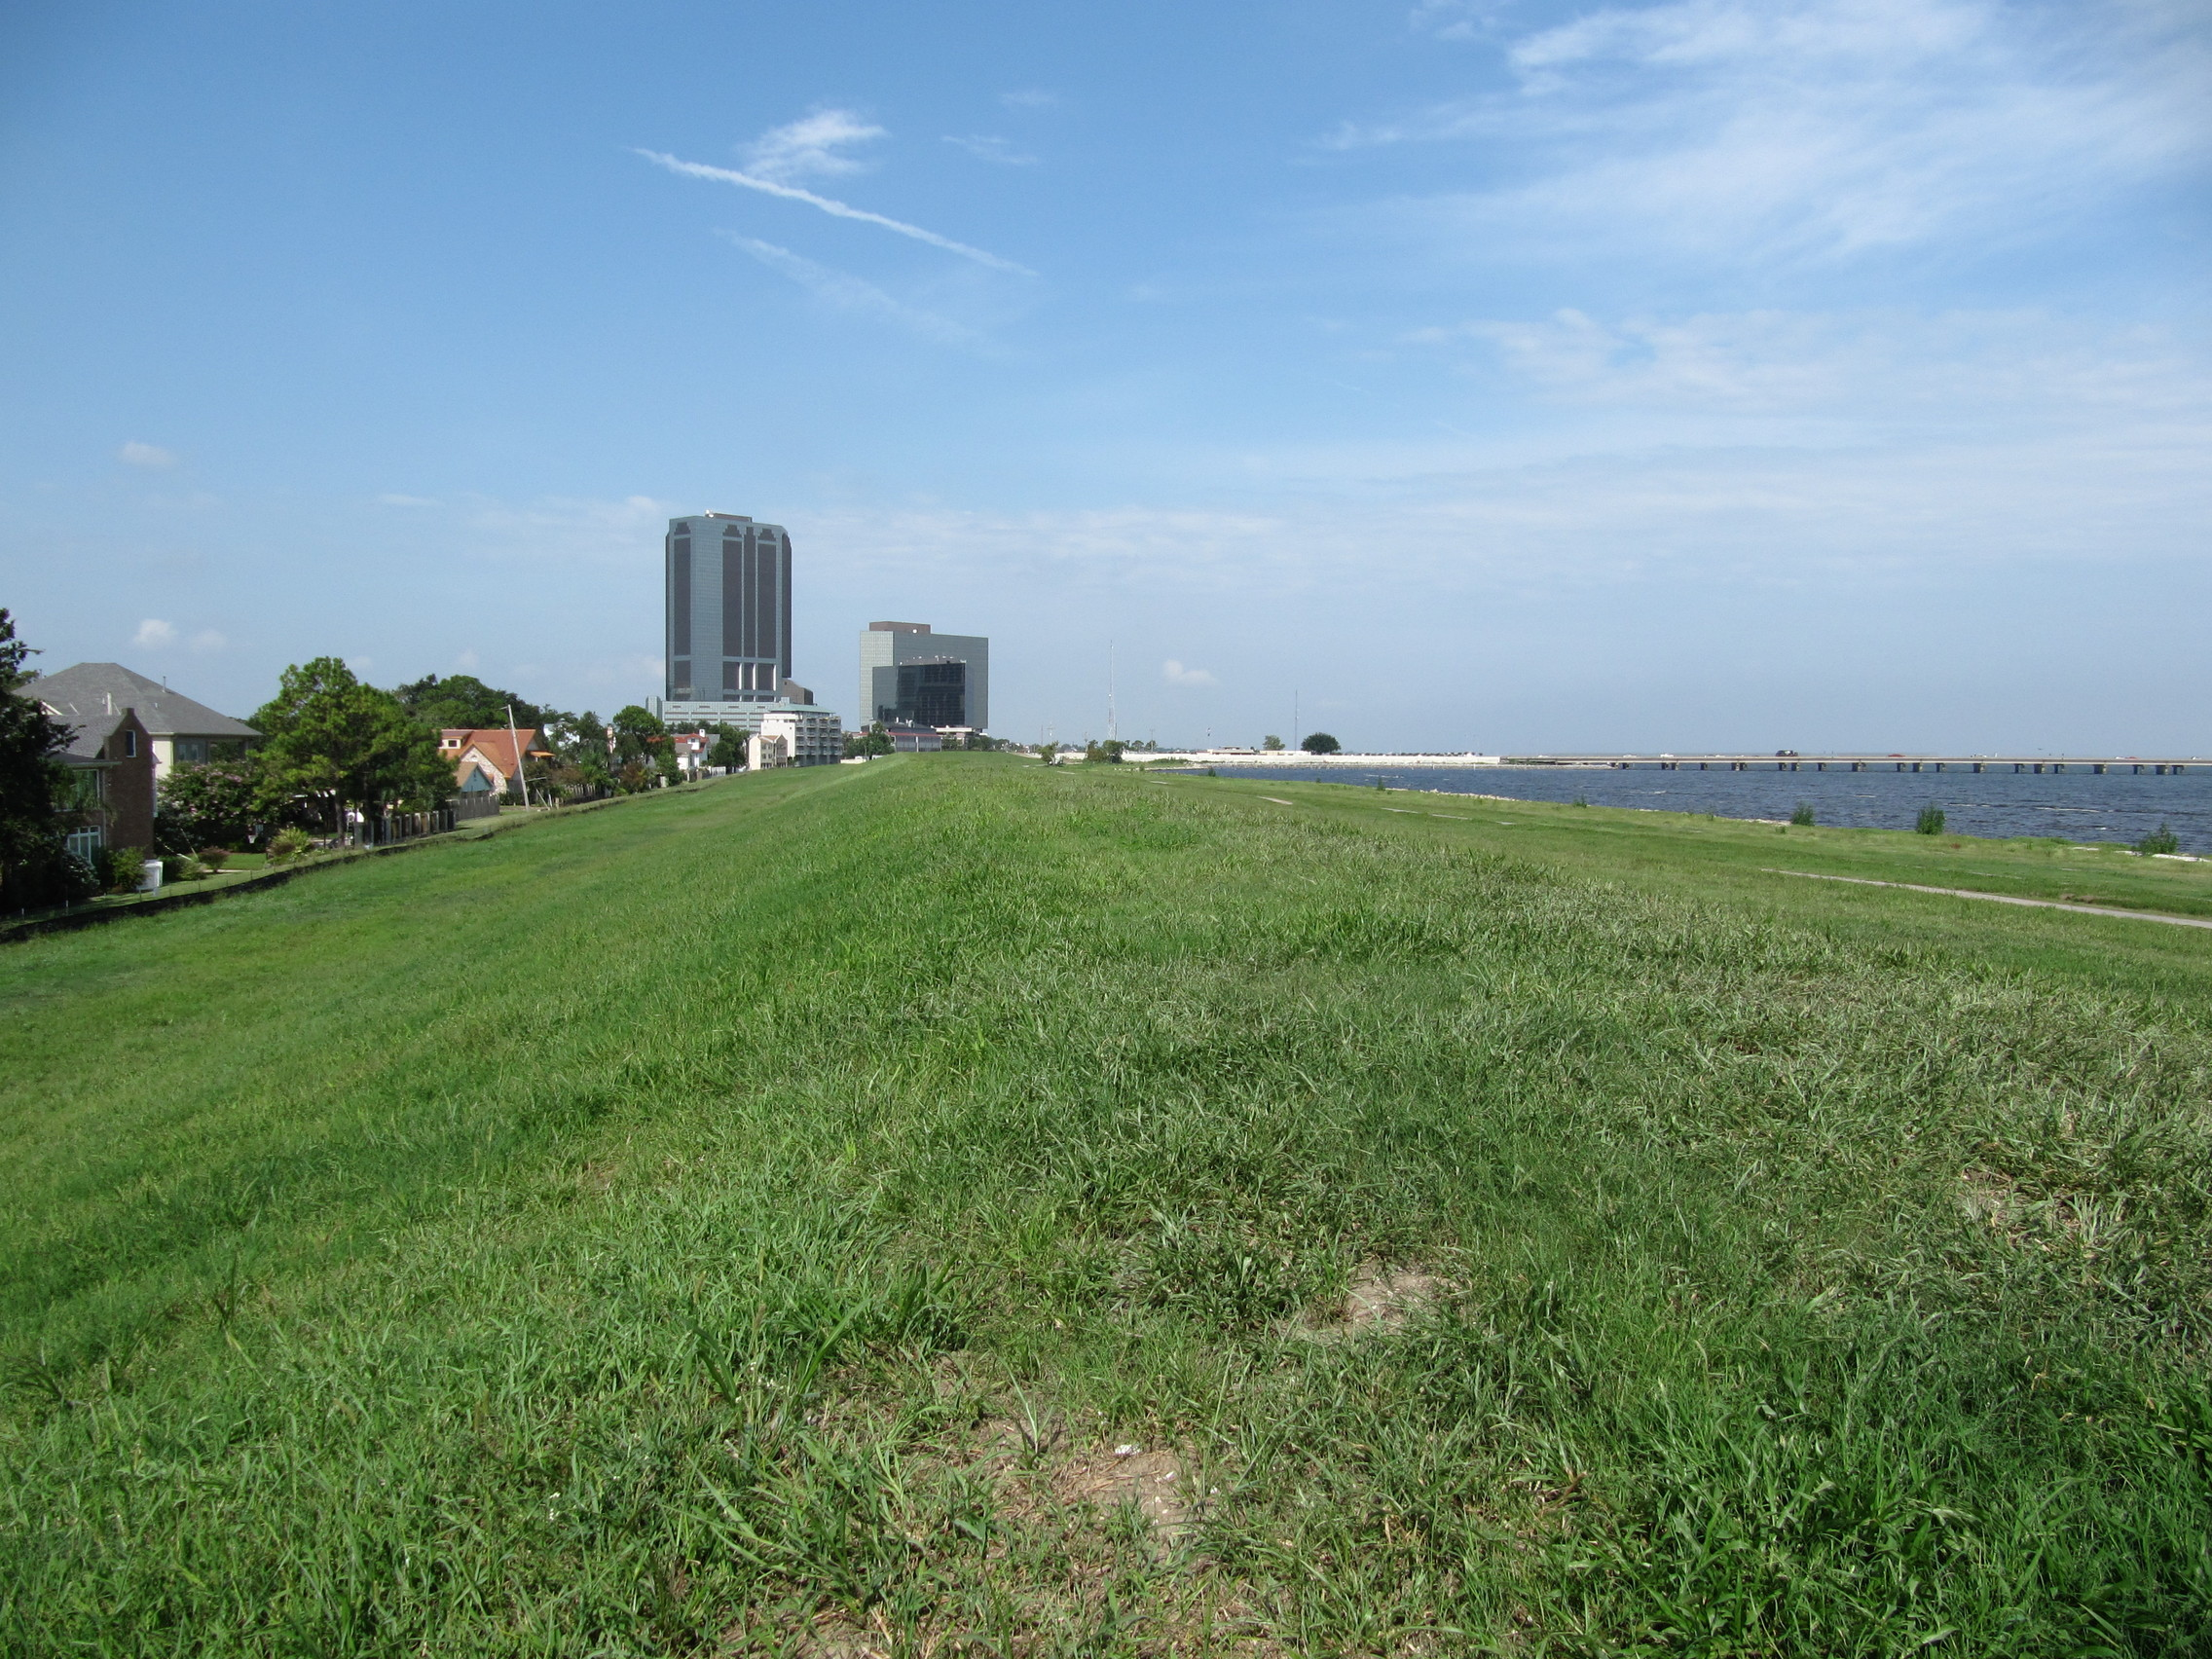
\includegraphics[width=1.0\textwidth]{images/GrassyLakeLevee.jpg}
  \end{minipage}
  \begin{minipage}{0.49\textwidth}
    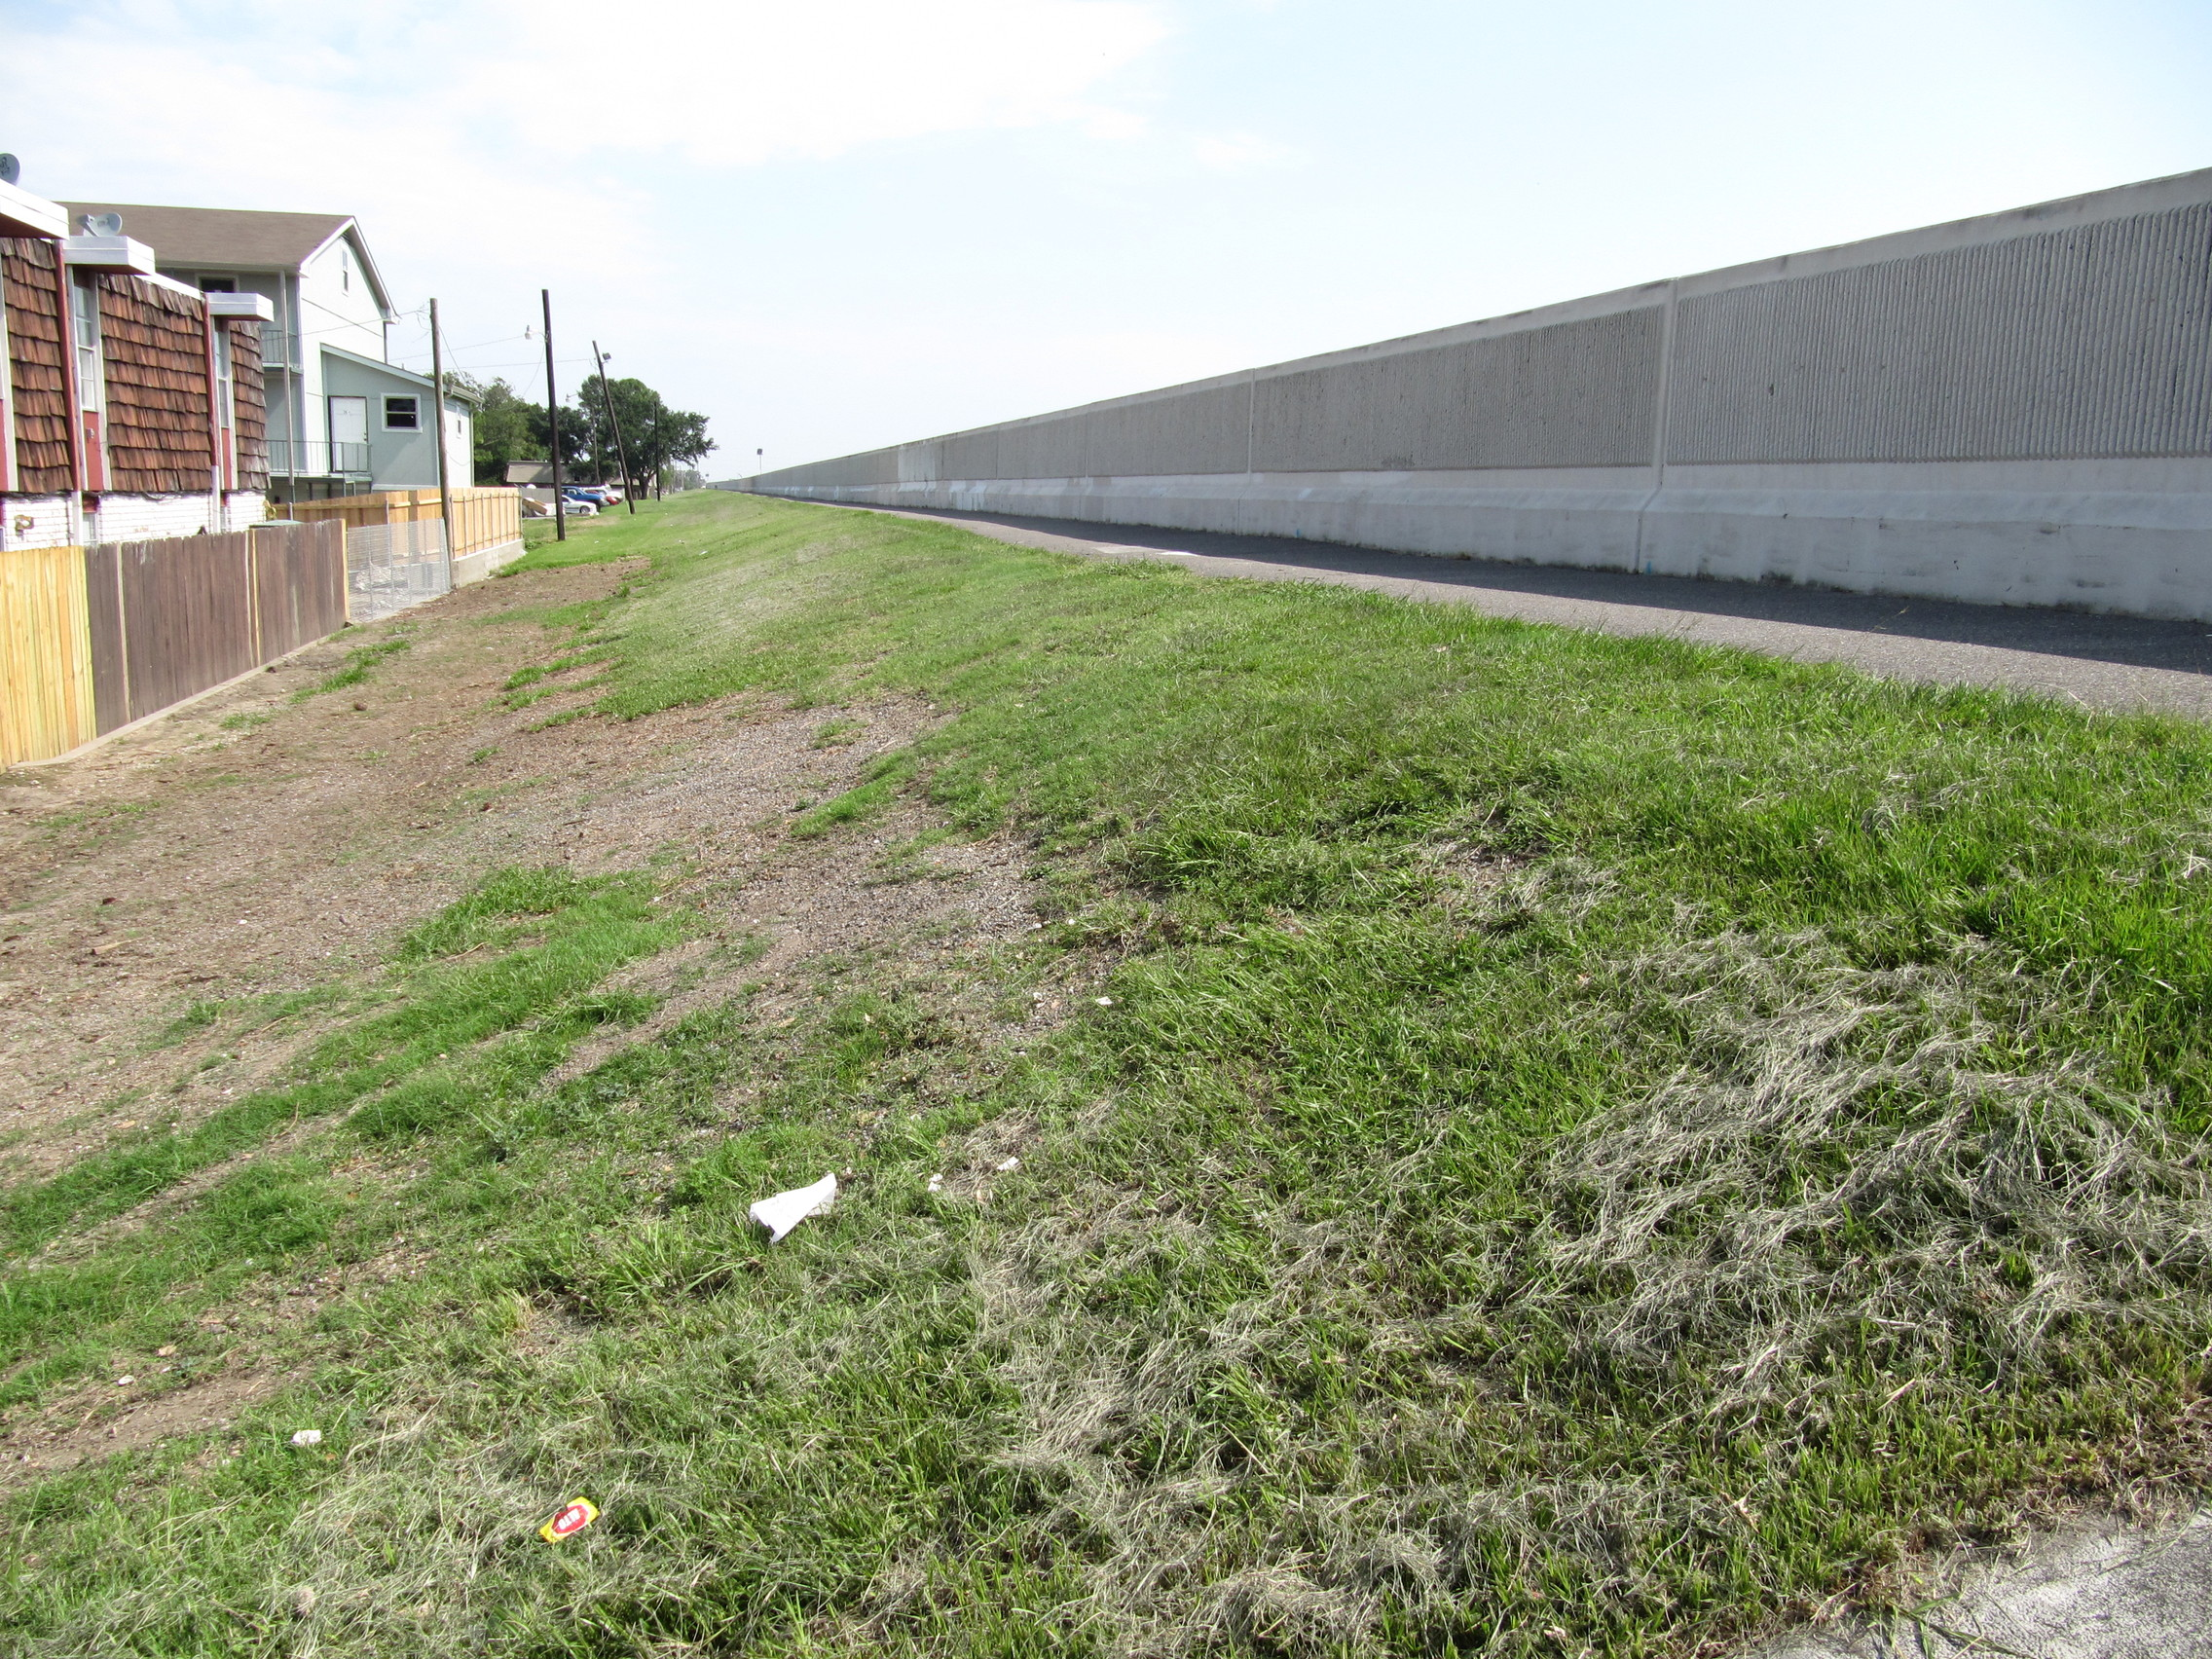
\includegraphics[width=1.0\textwidth]{images/DryLeveeWithRetainingWall.jpg}
  \end{minipage}
    \caption[Levees in New Orleans, LA]{(Left) An earthen lake levee in New Orleans, LA. (Right) An earthen levee with a temporary cement wall protecting a residential neighborhood in New Orleans, LA.}
    \label{figure:levees}
\end{figure}



\begin{figure}[t]
  \centering
  \begin{minipage}{0.99\textwidth}
    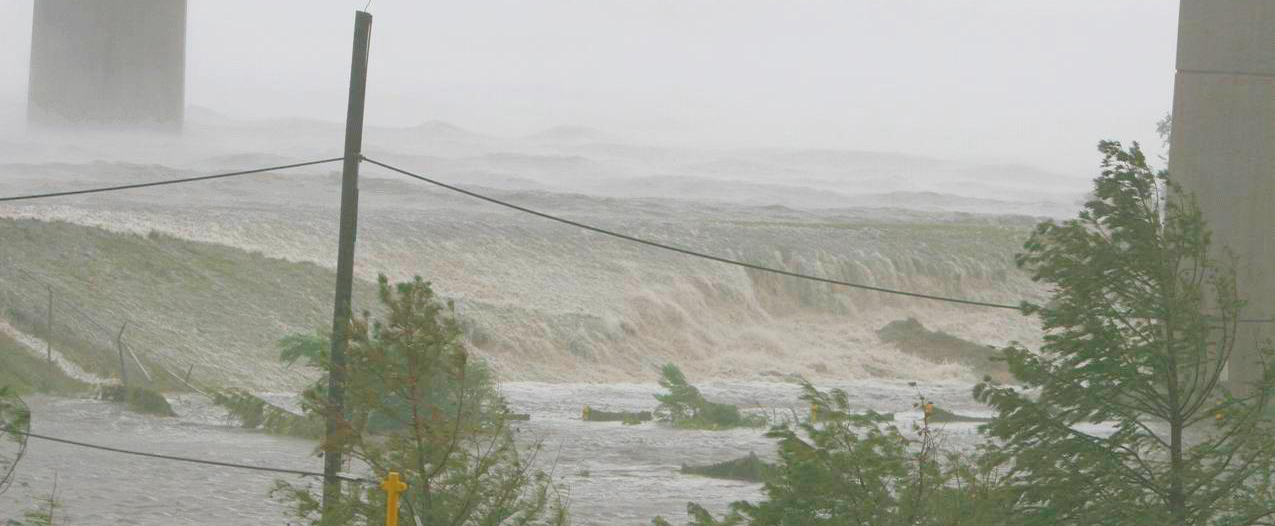
\includegraphics[width=1.0\textwidth]{images/zimmie_Picture2b_crop.jpg}
  \end{minipage}

  \begin{minipage}{0.99\textwidth}
    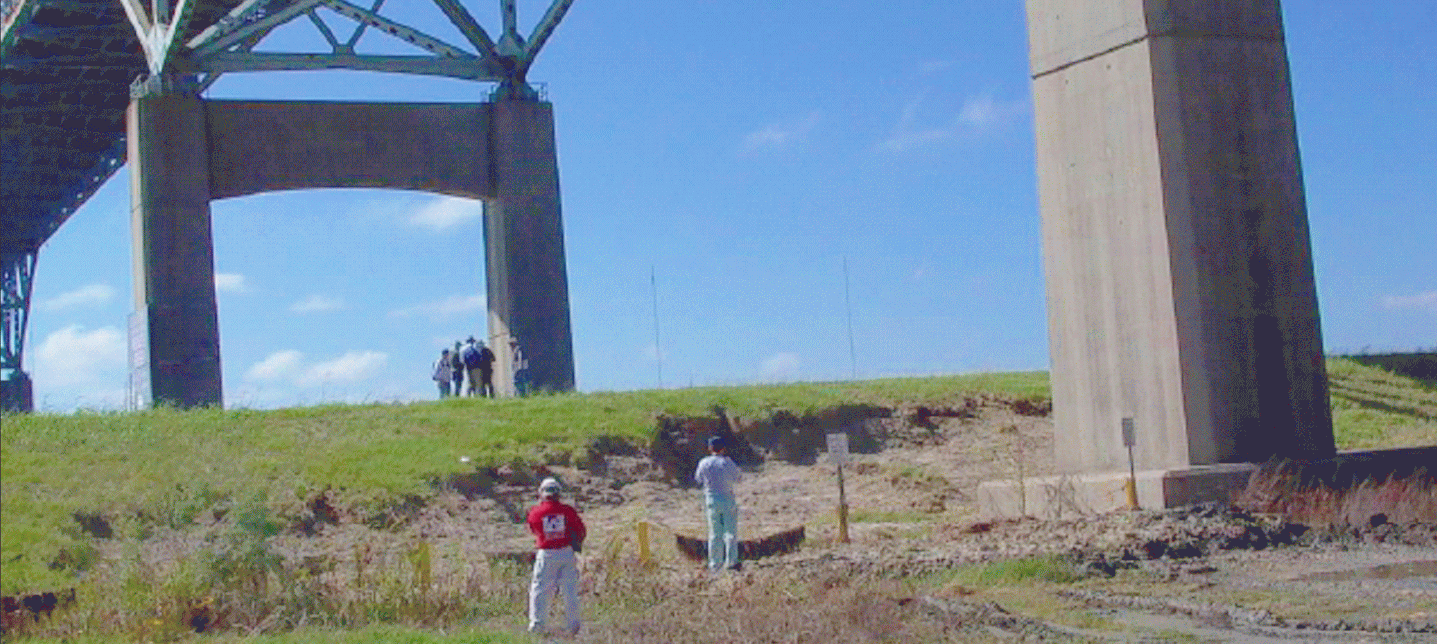
\includegraphics[width=1.0\textwidth]{images/zimmie_Picture1b_crop.png}
  \end{minipage}
  \caption[An overtopped levee]{A levee that was overtopped for several hours during
    Hurricane Katrina but did not fail.  The dramatic gouging/scooping
    on the lower portions of the levee is due to increased waterflow at
    the base of the levee and the non-homogeneous nature of the
    embankment.}
  \label{figure:katrina_photos}
\end{figure}



\begin{figure}[t]
  \centering
  \begin{minipage}{0.99\textwidth}
    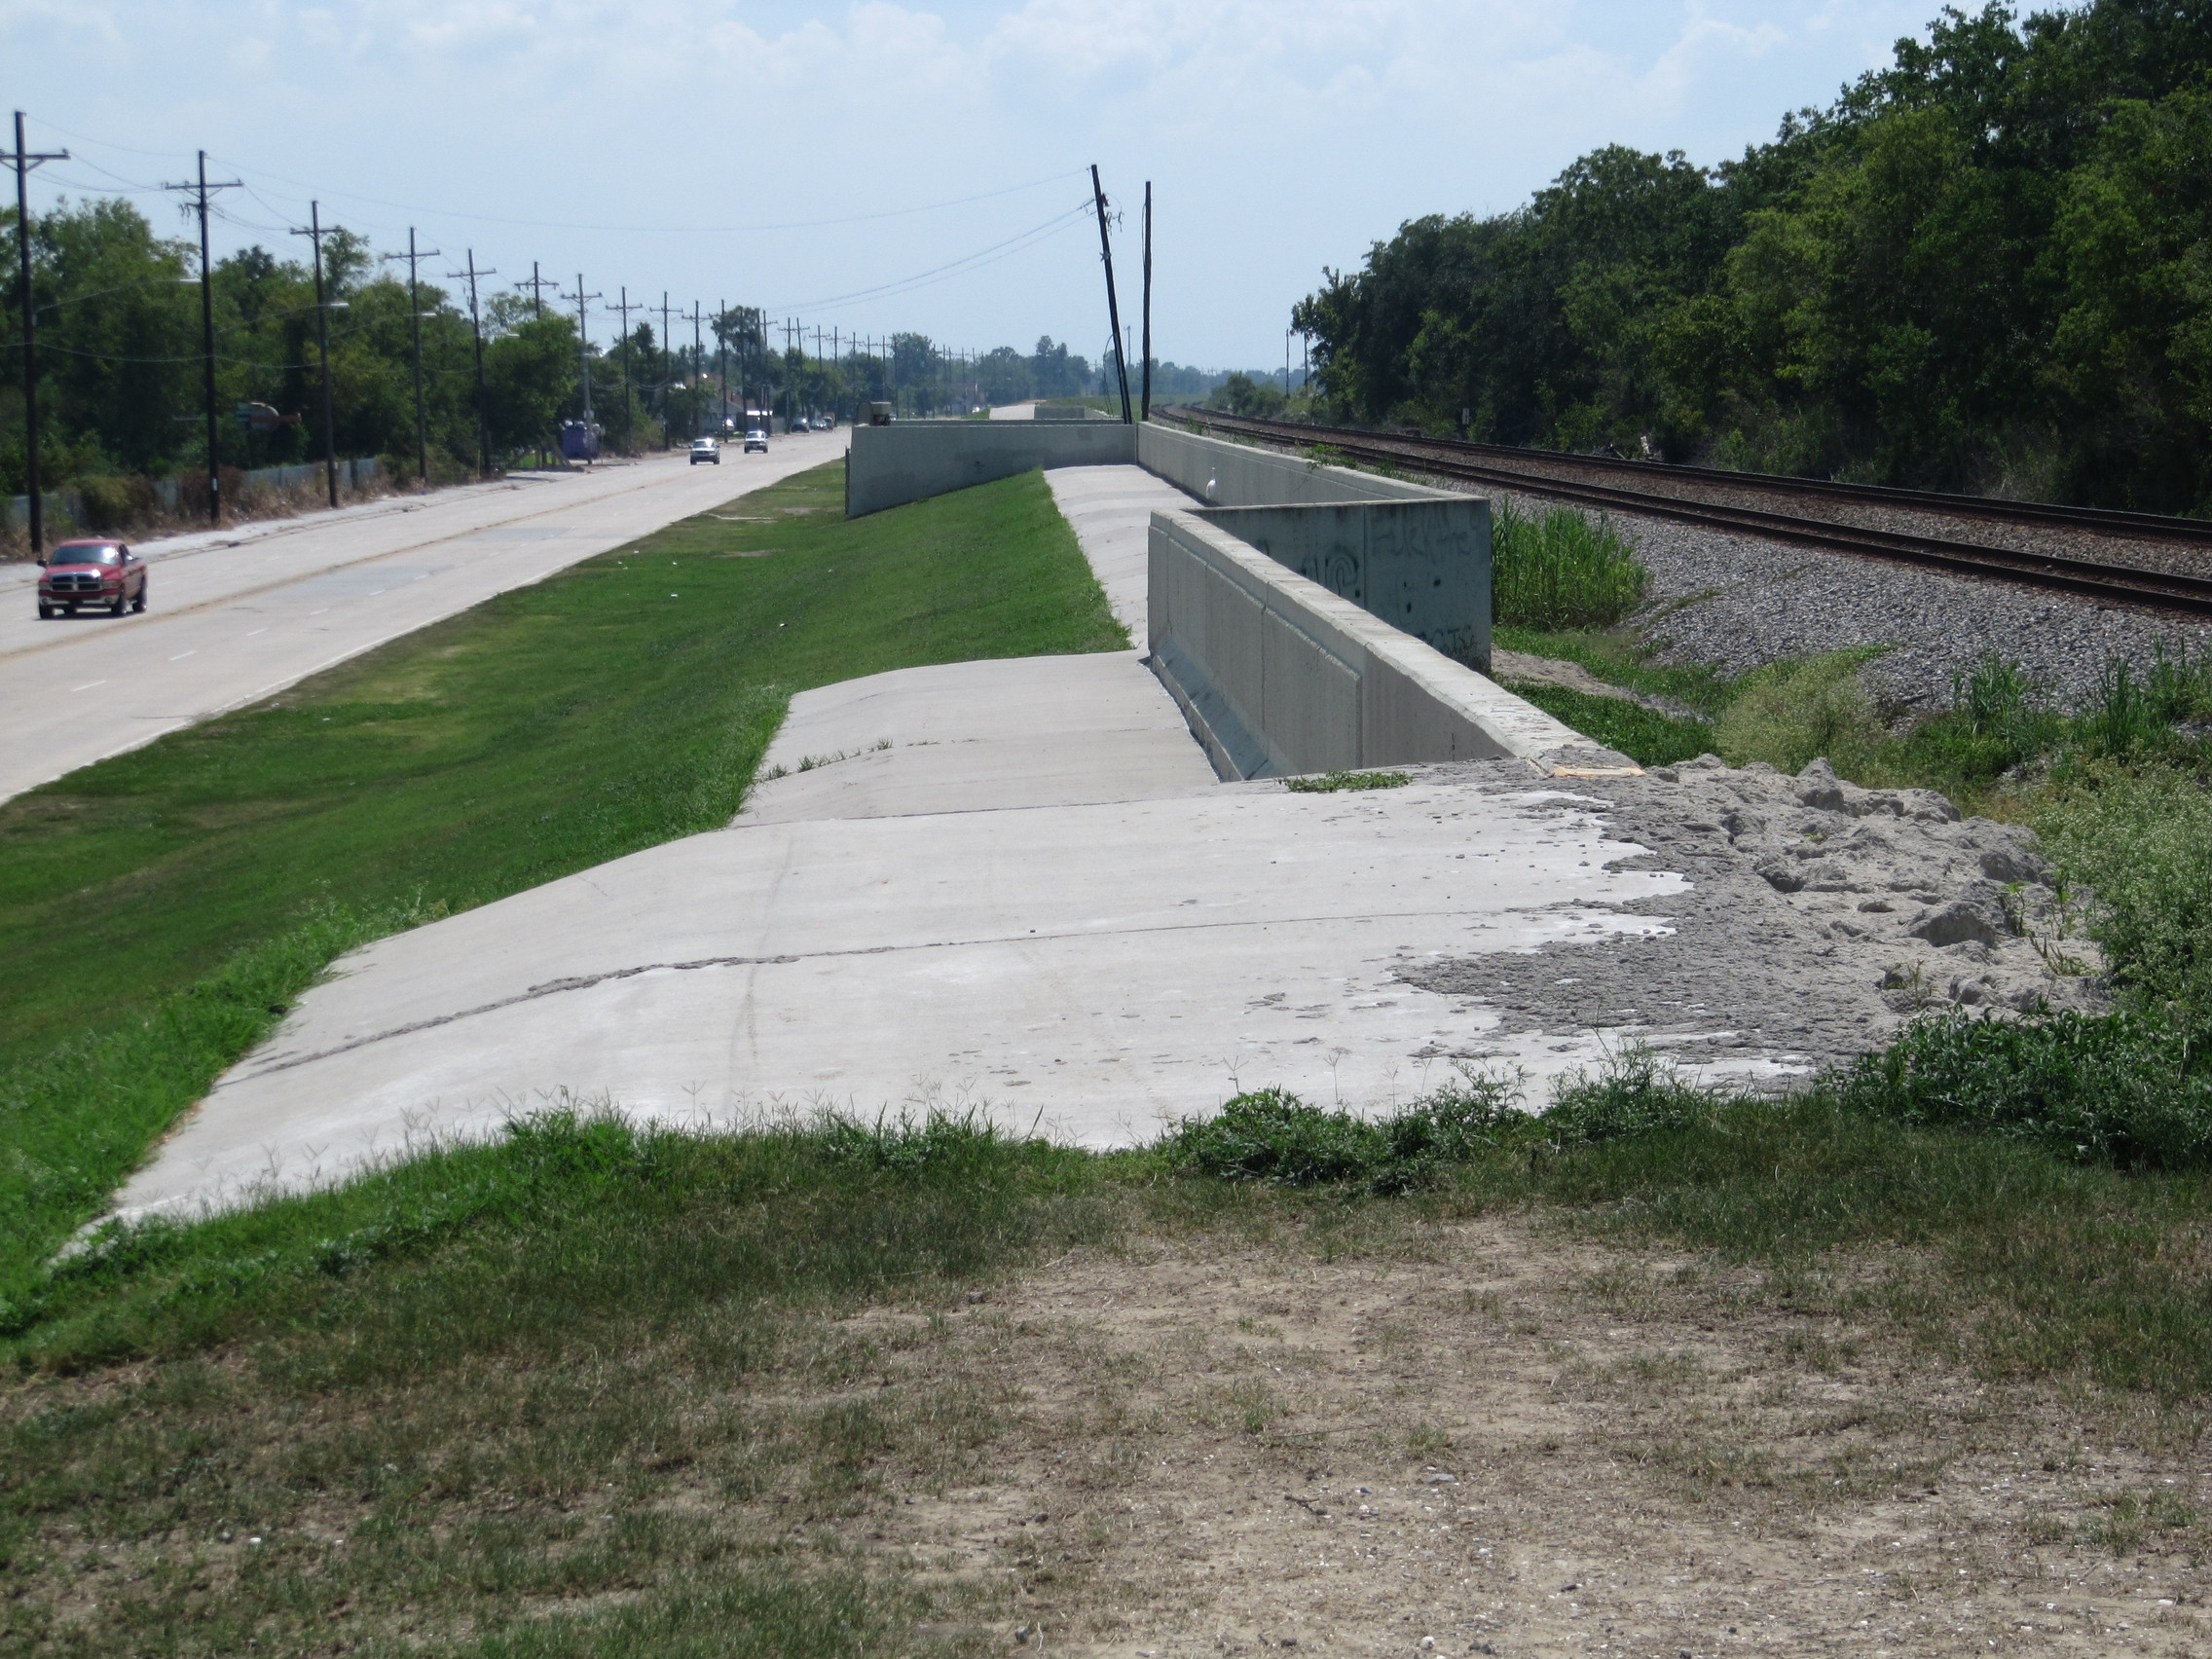
\includegraphics[width=1.0\textwidth]{images/RebuiltLevee.jpg}
  \end{minipage}
  \caption[A replacement cement wall]{A levee that failed during Hurricane Katrina and has been replaced with a temporary cement wall.}
  \label{figure:rebuilt_levee}
\end{figure}



% An understanding of the evolution of terrains makes possible the process of simulating it and, eventually, simulating its reverse.
% 
% A primary benefit of a deeper understanding of the evolution of terrain is the ability to simulate the reversal of the process. 
Given an original terrain and an eroded terrain, the ability to identify the series of operations on the original that formed the final eroded one is an interesting and challenging problem. One application of this forensic analysis is diagnosing earthen embankment (specifically levee) failure due to erosion, a primary motivation for this work.

Erosion in this thesis refers to hydraulic erosion, or the physical wearing away or breaking down of a material, usually a soil, by running water. 
% Other types of erosion include glacial and wind erosion. 
An earthen embankment is a sloped piece of land that is made 
% entirely 
of earthen materials, such as sand or clay. Earthen dams are walls of earthen material that hold a body of water over a long period of time, whereas earthen levees are two-sided embankments that protect objects on one side against periodic rising waters and crashing waves from the other (Figure \ref{figure:levee_diagram}). Some levees have non-earthen components, such as retaining walls or cores, made of less erodible materials like wood or clay. Some are replaced by cheaper materials, such as cement (Figure \ref{figure:levees}).
% , which is a hard (often cement) wall protruding from the top of it, or a core made of less erodible material, such as clay. 

Levee breach is the process whereby a channel through a levee forms due to high soil volume loss from hydraulic erosion, allowing water to pour through. Once breach has occurred, the failure of the levee is imminent. The time of breach is usually defined as the moment when the headcut (the very edge of the eroded channel) reaches point C in Figure \ref{figure:levee_diagram}, where the crest and the downslope meet. At this moment, an erosion channel that had been making its way across the crest widens and becomes a freeway for waterflow.
Levee breach and failure are most often caused by overtopping, the occurrence of water flowing over the crest of the levee, usually caused by high waves during a storm surge.

There are other methods for protecting levees against failure. Planting grass on the levee surface slows the rate at which erosion cuts channels in it. Levees can also fail by a process known as piping, or internal (subsurface) erosion, caused by water permeating the surface and eroding away the levee's foundation. A clay core works to mitigate this process, as does the use of geosynthetic materials through the body of the levee.

After a
catastrophe involving levee breach, such as the tragedy in New Orleans
during Hurricane Katrina, civil engineers attempt to piece together
the causes of the failure, usually seepage and/or
overtopping \cite{SENATE_REPORT} (Figure \ref{figure:katrina_photos}). 
% 
% \fbox{DEFINE OVERTOPPING}
% 
Forensic analysis of the cause of these failures is becoming more and more critical in assessing levee construction and safety, and its automation
makes this necessary process
more accessible.
%  faster and cheaper. 
% 
In addition, studying the erosion process that causes this failure in depth, including the formation of breach channels, the velocity and behavior of water, and the rate of the breach event, can lead to better levee construction and modeling, and is a primary motivation for the general purpose modeling problem presented in Section \ref{section:ModelingTerrainSurfaces}. A better understanding of the formation of the terrain surface and a better model for it go hand-in-hand.


Historically, there are many examples of levee failures, such as those by levees surrounding New Orleans during Hurricane Katrina (Figure \ref{figure:rebuilt_levee}).  Perhaps one of the most famous failures of an embankment dam by overtopping was the 1889 Johnstown, PA dam failure which killed more than 2000 people, left thousands homeless, and transformed the prospering city of Johnstown into a virtual wasteland \cite{Schnitter}.  Numerous other examples can be cited, but it is clear that such failures can cause serious loss of lives and economic disaster. Also, flood damage in the US cost \$50,000,000,000 in the 1990s \cite{FloodDamageData}. 
This largely unnecessary loss of money and lives can be mitigated with more detailed and accurate methods for studying and analyzing levee failures.
% Better understanding the ways in which earthen structures that are designed to help protect against flooding fail is an important step toward preventing this largely unnecessary loss of money and lives.
Erosion is such a fundamental and devastating natural process that representing terrain data by mimicking it is essential. One attempt to do so, using the drill operator, is presented in Chapter \ref{chapter:DrillOperator}.
% One which facilitates the study and analysis of erosion of levees leading to their failure involves the formation of a detailed hydraulic erosion simulation.


This thesis presents, in part, the work of a research group aiming to automate the diagnostic process of levee failure analysis by performing a detailed study of the levee geometry.
% , represented as one or more DEMs.


\begin{figure}[t]
  \centering
  \begin{minipage}{0.99\textwidth}
    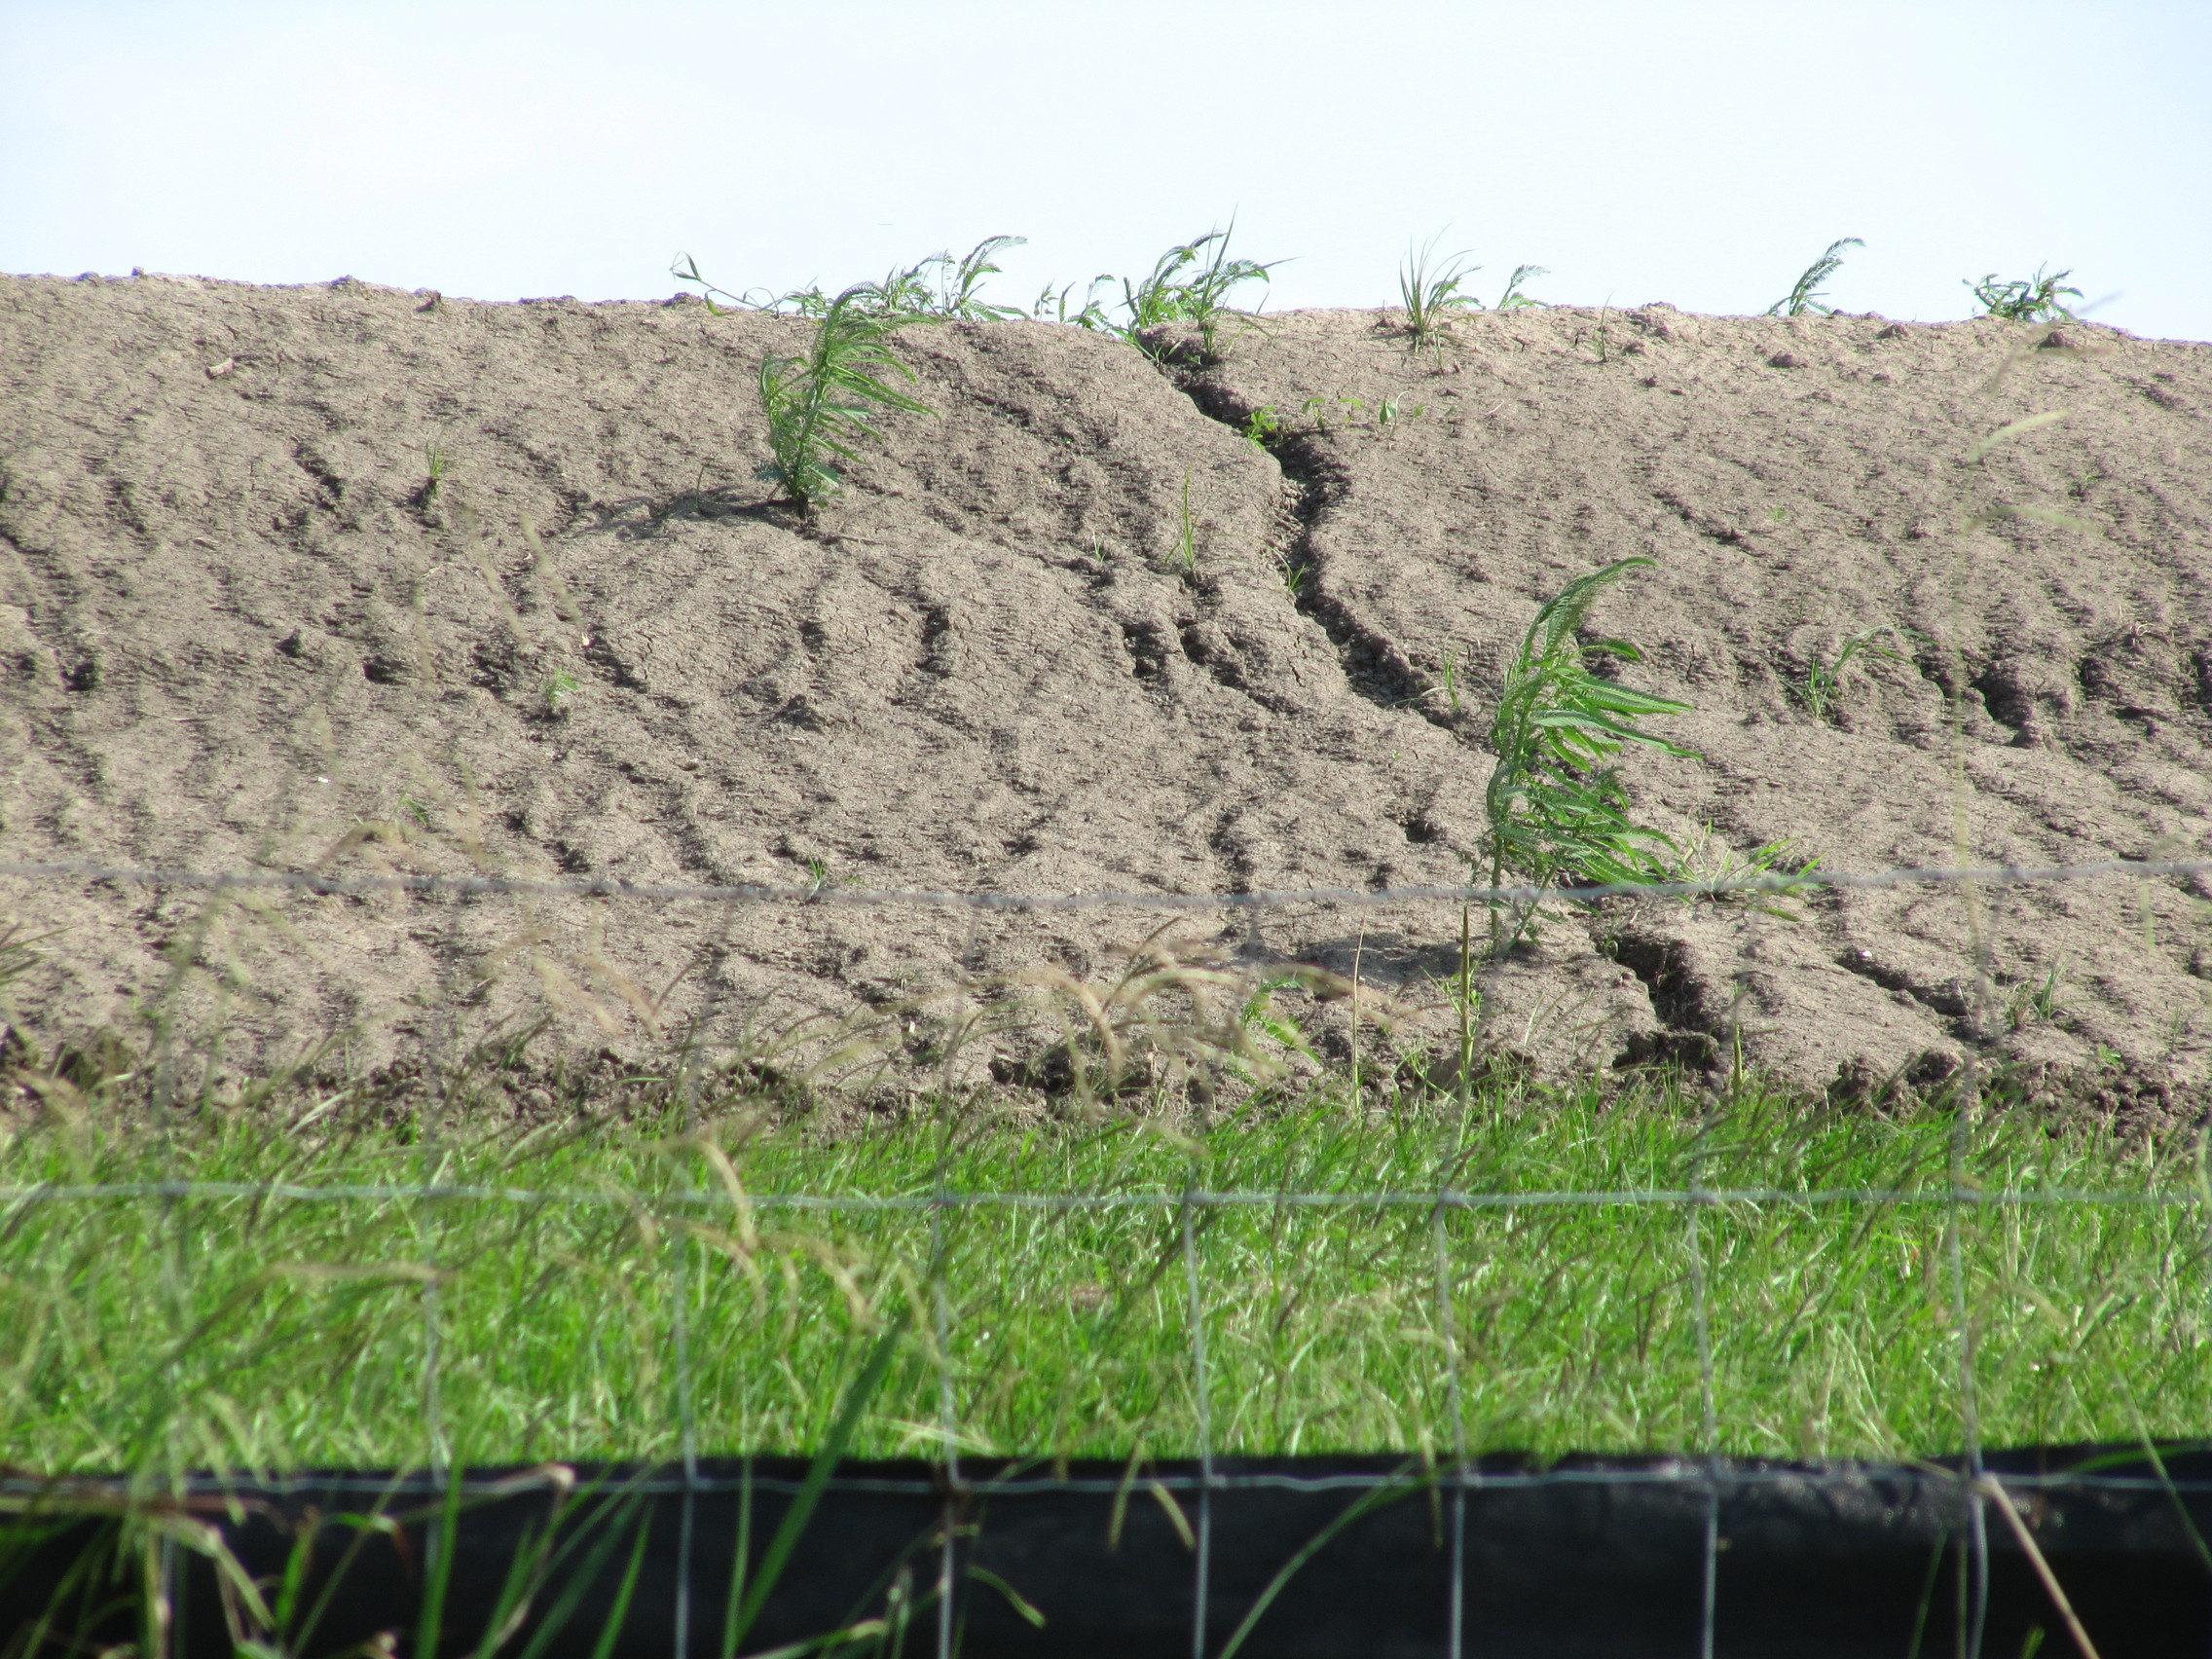
\includegraphics[width=1.0\textwidth]{images/RillsAndGullies.jpg}
  \end{minipage}
  \caption[Eroded channels on an earthen embankment]{An earthen embankment with eroded channels dug out of it.}
  \label{figure:rills_and_gullies}	
\end{figure}



This research focuses on small-scale erosion, which causes rills and gullies to form in the embankment (Figure \ref{figure:rills_and_gullies}). 
% During hydraulic erosion, other formations may develop in the soil, such as a head-cut, which is a sudden sharp cliff in the soil. 
% This formation erodes as a waterfall does as water runs over it. 
To study this, laboratory erosion experiments have been conducted at both 1-g and high-g levels (where ``g'' stands for gravitational units, or -9.8 $\dfrac{m}{s^2}$) in which a small-scale levee is constructed out of 
% Nevada 
sand and water is run over it.
% (figure \ref{figure:1GExperiments}). 
Results are recorded and the geometry of the surface of the levee, both before and after the experiment, is collected for comparison to simulation results. 
% scanned with a LIDAR scanner for use as input to our group's erosion simulation.
%  (chapter \ref{section:ErosionSimulation}).

The group's primary goal has been the development of a detailed and accurate erosion simulation that models laboratory experiments of levee failure. 
Erosion is simulated on an initial levee geometry using Smoothed Particle Hydrodynamics (SPH), coupled with a hydraulic erosion model well-known in civil engineering literature, the erodibility index model. This simulation is validated using analysis of the geometry of the laboratory experiments, both visually and statistically. This thesis presents an analysis of these results.

% In order for automated forensic analysis of levee failures to be a reality, a method must exist for measuring the changes between before and after geometry of the levee surface that goes beyond simple elevation changes. 
% Toward this goal, a framework has been developed for
% % Toward this goal, I have developed a framework for
% detailed comparison of eroded terrains that introduces the notion of
% terrain distance, a measure of how dissimilar two terrain datasets are.
% Methods for measuring terrain distance using the terrain's fingerprint, as well as the general spatial and hydrographic properties of the terrain, are introduced in this thesis. This framework is used to judge the overall accuracy of the group's results, the accuracy of the drill operator representation, and methods for determining the optimal channel network, while taking into consideration only the most important characteristics of the terrain surface.
% % combining channel network and terrain characteristic
% % distance metrics. This set of characteristics is the terrain \emph{fingerprint} (chapter \ref{section:FingerprintingATerrain}), and it governs a series of metrics that measure the dissimilarity between the drainage networks of two terrains (chapter \ref{section:DissimilaryMetrics}).

% MOVE THIS TO THE SIMULATION SECTION!!!!!

% \begin{figure}[t]
%   \centering
%   \begin{minipage}{0.98\linewidth}
%   \begin{minipage}{0.355\textwidth}
%     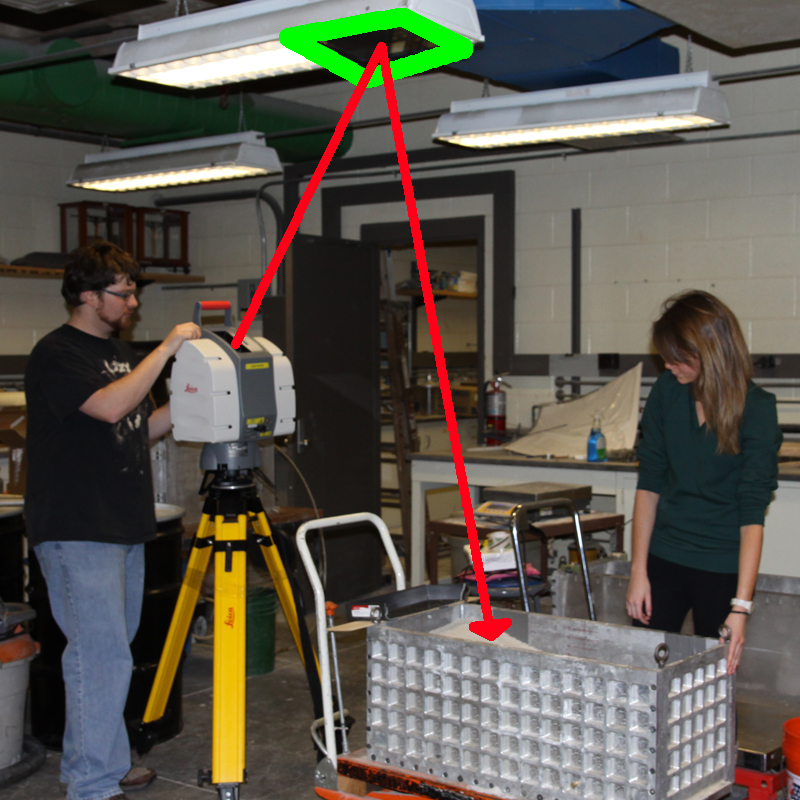
\includegraphics[width=\textwidth]{images/scanner_setup_small_annotated.jpg}
%   \end{minipage}
%   \begin{minipage}{0.635\textwidth}
%     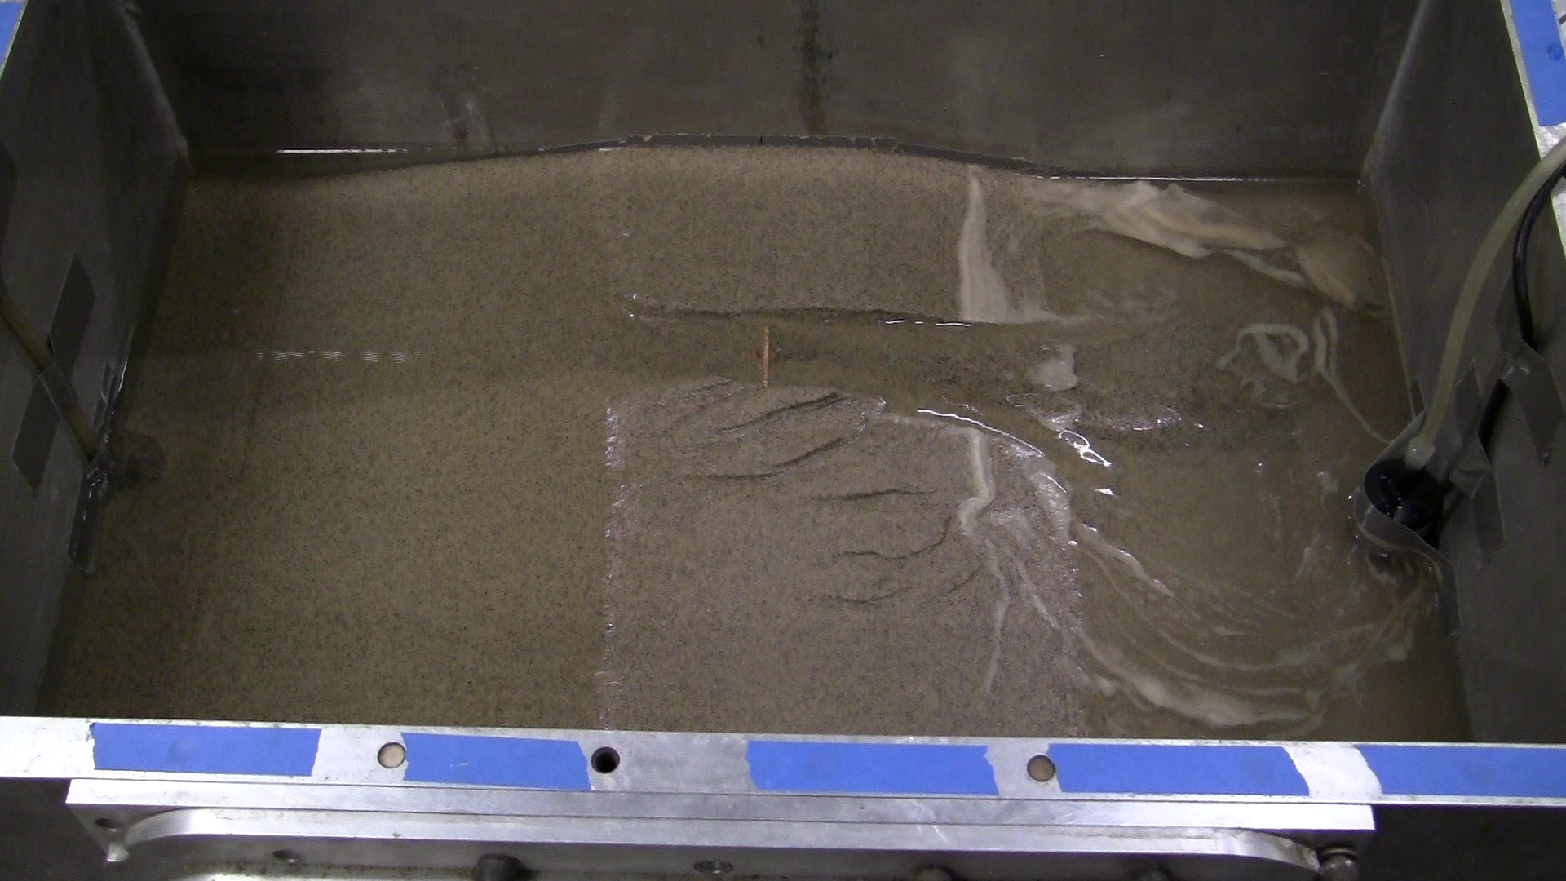
\includegraphics[width=\textwidth]{images/sand-10mins-phy-test.png}
%   \end{minipage}
%   \end{minipage}
%   \caption[Experimental setup of real world experiments]{\label{figure:1GExperiments} Left: LIDAR scanner setup, where LIDAR beams are shot off of a mirror placed on the ceiling and hit the surface of the levee model. Right: An image from the 1-g experiment, in which water flows left to right. A deep channel has clearly formed along the down slope of the levee model.}
% \end{figure}

\section{Data Manipulation and Exploration}

Spatial datasets are more useful if there exist methods for their exploration and manipulation. This thesis presents a system for large-scale group interactive problem solving using inexpensive, off-the-shelf laser pointers for this purpose. It is an example of an application with broad impact and utility that uses the models and simulation presented in Sections \ref{section:ModelingTerrainSurfaces} and \ref{section:ModelingLeveeFailure} for the educational purpose of allowing users to explore terrain data and view how slight changes in elevation values can have a strong impact on the behavior of water on the terrain.
% 
With this system, groups can, using an inexpensive and easy set-up, interactively explore terrain and hydrography data. The system allows each laser pointer to be uniquely identified among its peers by taking advantage of the fact that many inexpensive lasers leak infrared light as they do not include effective IR filtering. 

Since it is possible to uniquely identify each laser pointer, the system can be used for multi-user problem solving and data exploration. This work presents an application that displays an input terrain surface and allows the users to explore the data in a variety of ways. The system allows many users to each select their own individual actions using a button-based user interface. These actions include moving the camera, dropping rain on the surface, and manipulating elevation values along the surface of the terrain. The interactive-time nature of the application allows users to make changes to the terrain and see how the hydrography is effected immediately.

% Also presented in this work is a series of other applications using this technology, including games and emergency response programs.

\section{Contributions and Outline of Thesis}

% \fbox{THIS SECTION WILL BE DOUBLE CHECKED LATER}

This thesis presents the following contributions:

\begin{enumerate}
  \item The \emph{drill operator}, which mimics the process of drilling out a section of the terrain
%   \begin{enumerate}
%     \item An investigation of the effect of various drill shapes on the accuracy of the drill representation
    \item A compression scheme based on the \emph{drill operator} and an analysis of its compression ratios and accuracy
%     \item A method for post-processing terrain data to increase accuracy of \emph{drill operator}.
%     \item A method for \emph{machining} the terrain, applying finer and finer drills to the surface.
%   \end{enumerate}
%   \item A set of distance metrics that allow for the comparison of terrains
  \item The identification of various characteristics of a terrain surface, called the terrain's \emph{fingerprint}, that allow for comparison and analysis of terrain data
%   \begin{enumerate}
%     \item Channel width and depth fields
%     \item Channel meander field
%     \item Junction balance field
%     \item Pixel load field (intuitively, measure of importance of pixel)
%   \end{enumerate}
  \item An application of the Earth Mover's Distance to the probability distributions created by the fingerprint, allowing for measuring terrain dissimilarities
  \item A method of weighting terrain pixels when extracting the drainage network
%   \item A method for selecting a threshold for channel network extraction that allows for closer correlation between the channel networks of sequential terrains
  \item The segmented height field (SHF), a data structure designed for the volumetric representation of layered soil models
  \item A method for tetrahedralizing the SHF to form a closed tetra mesh for rendering and conversion to an SPH grid
%   \item A pipeline for capturing terrain surface data in a laboratory environment and converting it to the SHF
  \item Examination of the results from a series of erosion simulations on levee models
  \item A system for collaborative group interaction for data exploration on a large scale display using laser pointers
  \item A data exploration and manipulation educational application using the laser pointer system to explore and manipulate terrain surface data for educational purposes
\end{enumerate}


% \fbox{THIS NEEDS TO BE UPDATED}
This document is organized as follows: Chapter \ref{chapter:DrillOperator} presents the hydrography channel network extraction method used in this work, and a new representation of the terrain surface, the drill operator.
To determine the accuracy of the drill operator, several metrics for measuring terrain dataset distances are discussed.
Also presented is a compression scheme using this new representation, and a discussion regarding future directions of the drill operator.
Chapter \ref{chapter:FingerprintingATerrain} presents a definition and description of the terrain fingerprint, including the hydrographical characteristics that make it up, and its use in conjunction with the Earth Mover's Distance as a measure of dissimilarity between datasets.
Chapter \ref{chapter:ErosionSimulation} presents the results of several laboratory experiments modeling erosion on a levee surface, as well as the details of an accurate simulation of erosion using SPH, including an analysis of results.
Finally, Chapter \ref{chapter:TerrainDataExploration} presents a system for exploring and manipulating terrain data in a large-scale group-based setting, an application of the work in this thesis focused on its educational prospects. 
Chapter \ref{chapter:ConclusionAndDiscussion} draws a series of conclusions drawn from the work in this thesis, and a discussion of various applications of this work.


% , and its applications of it are presented in Chapter \ref{chapter:UsingTheDrillOperator}. Chapter \ref{chapter:TerrainDistances} introduces several metrics for measuring the distance between two terrain datasets, and Chapter \ref{chapter:FingerprintingATerrain} presents a definition and description of the terrain fingerprint. Chapters \ref{chapter:ErosionModeling} presents the results of several laboratory experiments modeling erosion on a levee surface, and Chapter \ref{chapter:ErosionSimulation} presents the details of an accurate simulation of erosion using SPH, including an analysis of results. Finally, Chapter \ref{chapter:TerrainDataExploration} presents a system for exploring and manipulating terrain data in a large-scale group-based setting, an application of the work in this thesis focused on its educational prospects. Chapter \ref{chapter:ConclusionAndDiscussion} wraps up with a series of conclusions drawn from the work in this thesis, and a discussion of ways in which this work can be extended.

\chapter{Prior Art in Terrain Modeling}
\label{chapter:TerrainRepresentations}



% FOOTNOTE THE ATTRIBUTIONS
\let\thefootnote\relax\footnote{Portions of this chapter previously appeared as: FIX \bibentry{stuetzle-TerrainDistances} }


The variation in GIS applications and the need for faster access and more compressibility 
% for terrain data 
has resulted in the development of a variety of data representations for elevation information. 
% Terrain data can and has been modeled in several ways, depending on the overlying application. 
Some only require that the surface of the terrain be modeled, while others need volumetric data stored as well.

% Real life terrain (deemed, in this thesis, to be the set of \textit{legal terrain}) differs from common data representations in a variety of ways. First, real terrain is not necessarily continuous everywhere. In fact, discontinuities litter the surface of the earth, from cliff faces and waterfalls to caves and tunnels. These discontinuities are difficult to represent with any spatial data structure. Second, because most terrain does not contain local minima, small pits that can collect water and prevent easy travel, legal terrain also lacks local minima. Error is inevitable during the surface data collection phase, and so oftentimes local minima are introduced where there should be none. Spatial datasets allow for this inaccuracy, with no mechanism for minimization or prevention. Thirdly, ideal terrain representations should contain formation information beyond that of strictly the spatiality of the data, closely tying the representation to the physics responsible for generating the terrain. When determining the accuracy and viability of common terrain representations, the ability to model legal terrains should be taken into account. Finally, an ideal terrain representation will allow for local data manipulation without effect on the global shape.

\section{Surface Representations of Terrain}
\label{section:SurfaceRepresentations}

For many applications, knowledge of only the surface of the terrain is sufficient. In computer graphics, surface data is used for many terrain generation techniques, including fractal generation and shallow water erosion simulations.
In each case, individual grid values are manipulated, requiring knowledge of only elevations along the surface. 
Like all models, rendering a terrain requires only the surface data, as well.

The method of terrain representation chosen can have a profound effect on the application it is used for. Walker et al. \cite{elevationDataEffects} demonstrate the way in which inaccurate terrain data may effect a seemingly unrelated application, atmospheric modeling. Small changes (i.e. errors) introduced into the data have a substantial effect on the results of atmospheric models.

% Most applications in computer graphics (terrain generation, rendering, simulation) and GIS (hydrography, dam siting, path planning) require knowledge of only the surface of the terrain. There are many representations that encode only the surface, including height fields, triangulated irregular networks (TINs), and Fourier functions.

\subsection{Height Fields}

\begin{figure}
  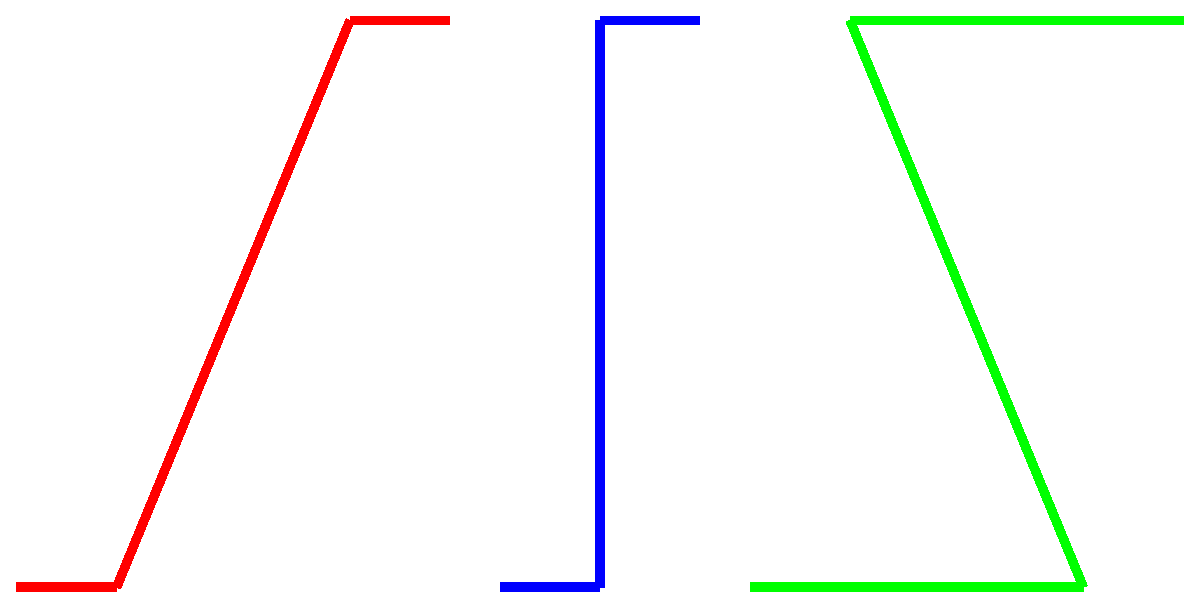
\includegraphics[width=0.99\textwidth]{images/TerrainShapes.eps}
  \caption[Various terrain formations too complex for surface representations]{\label{figure:TerrainShapes}Three possible terrain formations that are indistinguishable given spatial height field data: a positive slope (red), a vertical cliff face (blue), and an overhang (green). These formations are too complex for any surface representation to correctly model.}
\end{figure}

%Figure of each datasets
\begin{figure*}[t]
\centering
\begin{minipage}[b]{0.3\linewidth}
\begin{center}
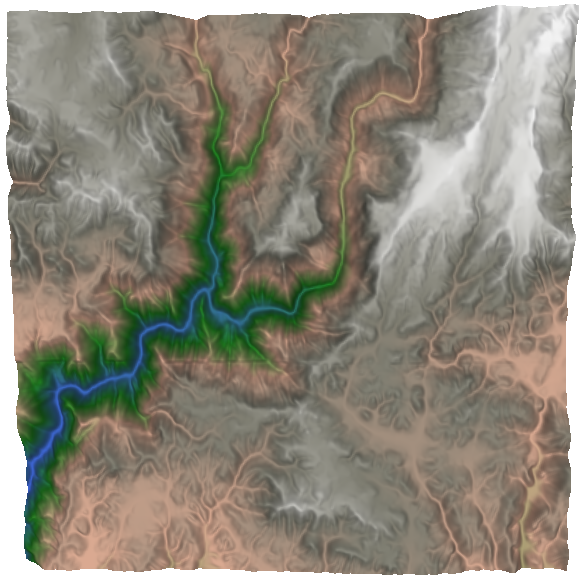
\includegraphics[width=\linewidth]{images/mtn1_normalized.png} \\
MTN1
\end{center}
\end{minipage}
%
\begin{minipage}[b]{0.3\linewidth}
\begin{center}
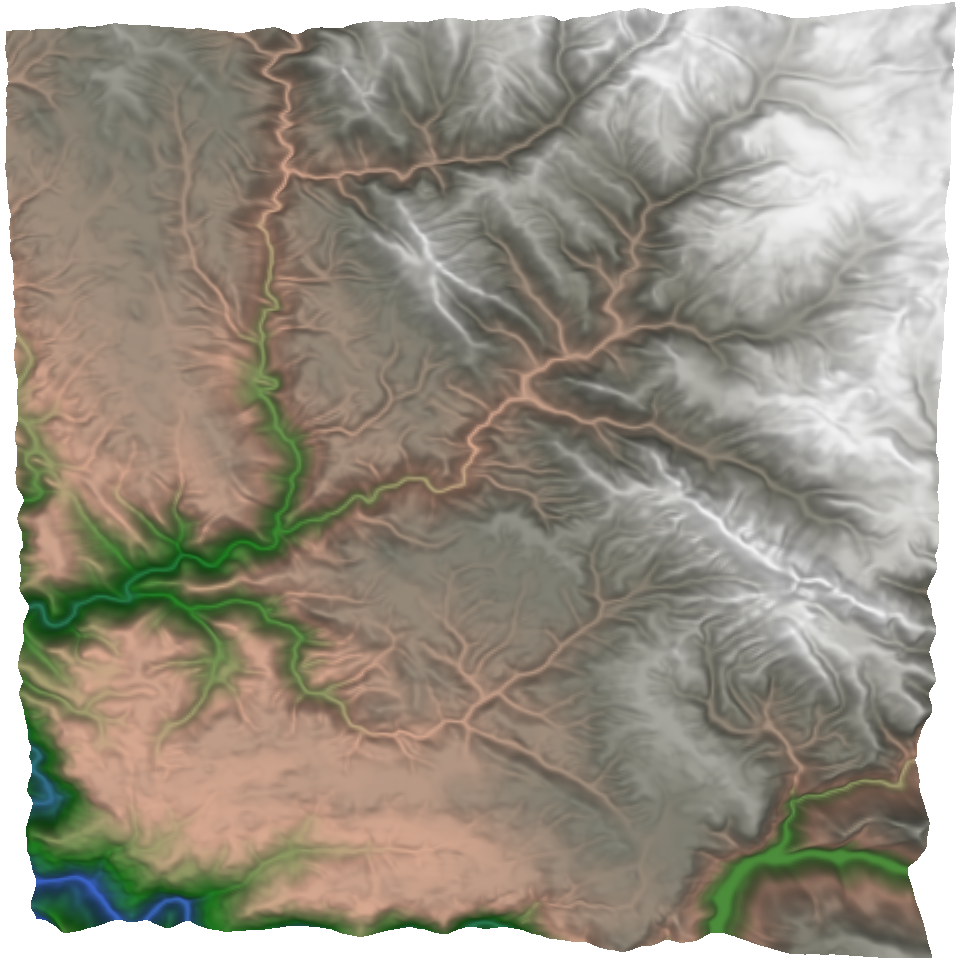
\includegraphics[width=\linewidth]{images/mtn2_normalized.png} \\
MTN2
\end{center}
\end{minipage}
%
\begin{minipage}[b]{0.3\linewidth}
\begin{center}
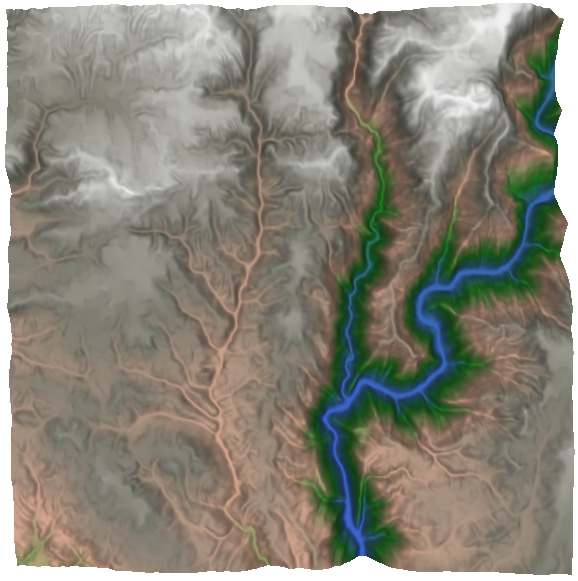
\includegraphics[width=\linewidth]{images/mtn3_normalized.png} \\
MTN3
\end{center}
\end{minipage} \\
%
\begin{minipage}[b]{0.3\linewidth}
\begin{center}
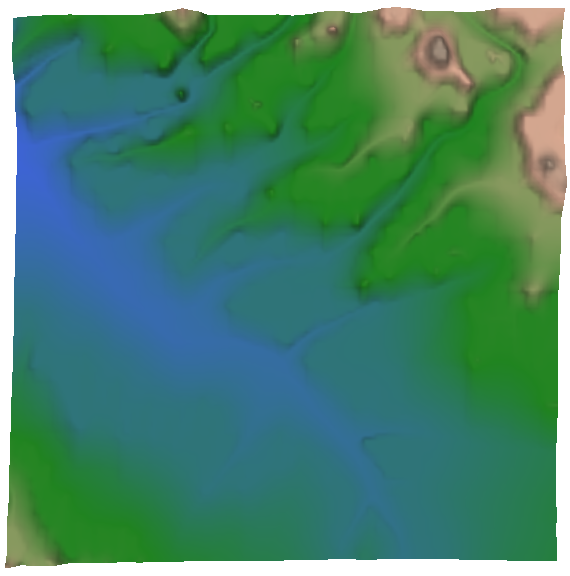
\includegraphics[width=\linewidth]{images/hill1_normalized.png} \\
HILL1
\end{center}
\end{minipage}
%
\begin{minipage}[b]{0.3\linewidth}
\begin{center}
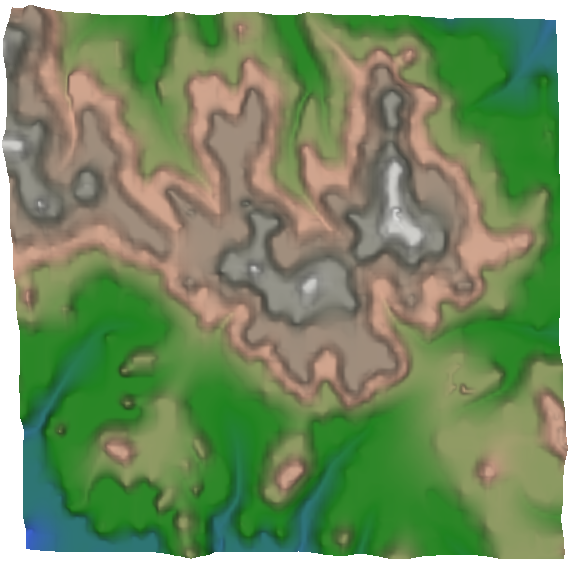
\includegraphics[width=\linewidth]{images/hill2_normalized.png} \\
HILL2
\end{center}
\end{minipage}
%
\begin{minipage}[b]{0.3\linewidth}
\begin{center}
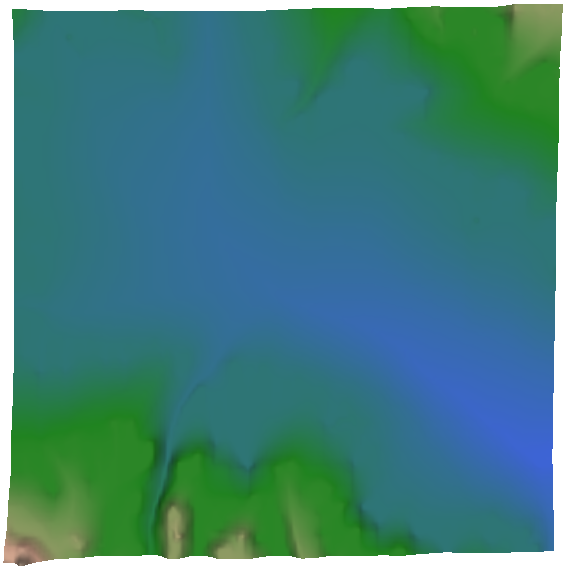
\includegraphics[width=\linewidth]{images/hill3_normalized.png} \\
HILL3
\end{center}
\end{minipage}
%
\caption[Six height field datasets used for analysis]{\label{figure:SixDatasets} Six $400 \times 400$ height fields used in this thesis for analysis, three mountainous datasets (top row) and three hilly datasets (bottom row). These are top-down views of each set, and color indicates elevation (normalized to the maximum elevation range of the set) measured in meters, transitioning from white at the highest elevations, to brown, then green, and then to blue at the lowest elevations. These datasets were first used by Inanc \cite{inanc-phd}.}
\end{figure*}

\begin{table}
\centering
\caption[Geological information regarding six datasets.]{\label{table:SixDatasetsInformation}Geological information regarding the six datasets used in this thesis, presented graphically in Figure \ref{figure:SixDatasets}. This table was first used by Lau and Franklin \cite{Lau-CAGIS}. }
\small{
\begin{tabular}{|c|c c|c c c|}
\hline
               &                  &                     & \multicolumn{3}{c}{Elevation in meters}      \\
DEM 		   & Cell name        & Cell Range          & Mean            & Standard Deviation & Range \\ \hline
\textit{HILL1} & \texttt{W111N31} & 401:800,1:400       & 1251            & 79                 & 1105:1610 \\
\textit{HILL2} & \texttt{W111N31} & 401:800,401:800     & 1548            & 134                & 1198:1943 \\
\textit{HILL3} & \texttt{W111N31} & 401:800,801:1200    & 1309            & 59                 & 1199:1699 \\
\textit{MTN1}  & \texttt{W121N38} & 1201:1600,1201:1600 & 712             & 146                & 219:1040 \\
\textit{MTN2}  & \texttt{W121N38} & 2801:3200,801:1200  & 847             & 152                & 330:1283 \\
\textit{MTN3}  & \texttt{W121N38} & 3201:3600,401:800   & 723             & 161                & 233:1021 \\
\hline
\end{tabular}
}
\end{table}


Height fields are matrices of evenly-spaced elevation values (each x,y coordinate has exactly one corresponding elevation). Each grid space is referred to from this point forward as a pixel. 
% Throughout this work, these elevations will be assumed to be whole integer values.
%  (which is not always the case, but has no 
In most applications in GIS, terrain is stored as a Digital Elevation Model (DEM), whose underlying representation is a height field. Due to their simplicity, height fields are often the least complex representation to work with. Many GIS algorithms have been optimized for elevation grids. The regularity of their grid structure and the simplicity of the representation itself make height fields ideal candidates for most applications, but they have shortcomings as well.

The accuracy of height fields is limited by the assumption that terrain is $C^{0}$ continuous everywhere,
%  and differentiable, 
which is rarely true.
Discontinuities are apparent in real terrain (e.g. the Grand Canyon), but the information necessary to represent them is lost when storing a matrix of elevation values. For instance, given the following matrix of elevations:

\begin{center}
  \begin{tabular}{c|c|c}
    24 & 23 & 12 \\
    \hline
    23 & 21 & 12 \\
    \hline
    24 & 21 & 11 
  \end{tabular} 
\end{center}

\noindent it is impossible to determine whether the slope between columns 2 and 3 is positive, undefined (vertical), or negative (an overhang), and so it is assumed to be positive in most applications. 
Examples of these three possibilities with regard to their surface shape is shown in Figure \ref{figure:TerrainShapes}.
% At coarse grid resolutions, this may force 
For many terrain formations, this is 
% correct, or at least 
sufficient.
% , but not always.

Height field data collection requires acquiring samplings of elevation values. Modern collection processes suffer from failure to adhere to the Nyquist Sampling Theorem \cite{nyquist}, which states that the sampling frequency of a set of data should be at least twice that of the data itself. Due to this and the lack of a representation of terrain that facilitates more accurate data collection, there is a great deal of terrain data that contains inaccuracies.

Figure \ref{figure:SixDatasets} shows a graphical representation of the six height field datasets that are used throughout this thesis. Three mountainous datasets and three hilly datasets are used, each a $400 \times 400$ grid of pixels with elevation values measured in meters. Notice that the mountainous datasets have very clearly defined channels (rivers) running through them, like veins. The hilly datasets, however, are low-frequency data with very few features and large, flat areas. 

\subsection{Triangulated Irregular Networks}

% \fbox{WILL ADD A FIGURE OF A TIN FROM ARCGIS}
 
TINs are triangulated terrain surfaces built of piecewise linear splines, and can be thought of as triangulated 
% grid-less 
three-dimensional points (or nodes) with stored or known connectivity.
TINs are often formed by triangulating a sampled set of points from a height field, thus allowing for a more compact representation.
TINs suffer from the same limitation as height fields because triangulated representations require that each node's (x,y) coordinate be unique and single-valued to generate a continuous surface (i.e., with $C^{0}$ continuity).

In addition, the accuracy of 
both height fields and TINs are dependent almost entirely on the resolution of the data points. Coarser resolutions have a profound and negative effect on the accuracy bound of the data (Gao \cite{gao:resolution}). This limitation can be somewhat mitigated by developing variable resolution, possible for both representations (such as in Abdelguerfi, et al. \cite{Abdelguerfi-HierTINs}, De Floriania, et al. \cite{DeFloriani-HTINs}, Bartholdi and Goldsman \cite{BartholdiAndGoldsman-HierTINs}, and Velho, et al. \cite{Velho-HierTINs}), but even this solution is limited. More data points requires more storage and introduces more sources of possible error. The trade-off of more data points means that finding a TIN-approximation of a given surface is complex. 
In fact, Agarwal and Suri \cite{Agarwal:1994:SAG:314464.314475} show that computing a piecewise linear $\epsilon$-approximation of a bivariate function (terrain surface) is NP-Hard. 

Additional information layers are often stored on top of height fields and TINs. Scalatos and Pavlidis \cite{Scarlatos:1990:HTU:949531.949559} represent hierarchical connectivity information for the TIN, because organizational scheme is important for algorithmic efficiency when using TINs. Similarly, Cignoni et al. \cite{Cignoni97representationand} present a hierarchical method for approximating a TIN with fewer triangles by greedily adding elements to the approximating set one at a time and recalculating the global error. Triangles in this system remember the overall error before and after their ``birth'' and ``death'' allowing for simple optimization.
Keller and Baru \cite{KellyAndBaru_GPLATES} present GPlates, a system for visualizing and manipulating plate tectonic data. The internal representation of the data is as 3D unit vectors, with the poles given [ 0 0 1 ] and [ 0 0 -1 ], to avoid the problem of having to assign a longitude to them. The actual elevation data is simply a height field, and plate boundaries are stored as polygons, or collections of elevation values. Baumann et al. \cite{Baumann:1999:HHD:792758.793044} present a hierarchical data structure that has been generalized for textured terrains. The data structure is essentially a generalization of k-d trees on a gridded terrain that can be applied to other terrain representations, such as TINs.

\subsection{Fourier Series, Splines, and Other Mathematical Models}

% \fbox{ADD AN IMAGE OF EACH KIND OF FUNCTION}

\begin{figure}
  \begin{center}
%     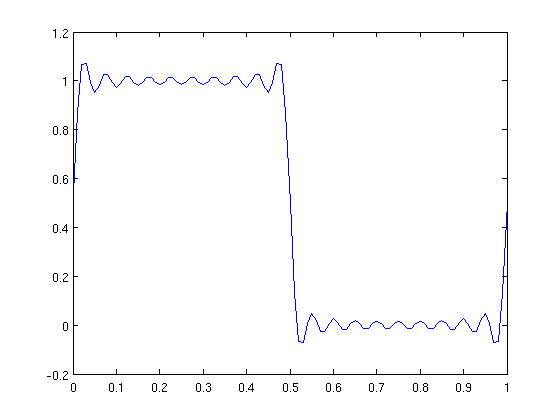
\includegraphics[width=0.5\textwidth]{images/Fourier_N20.png}
    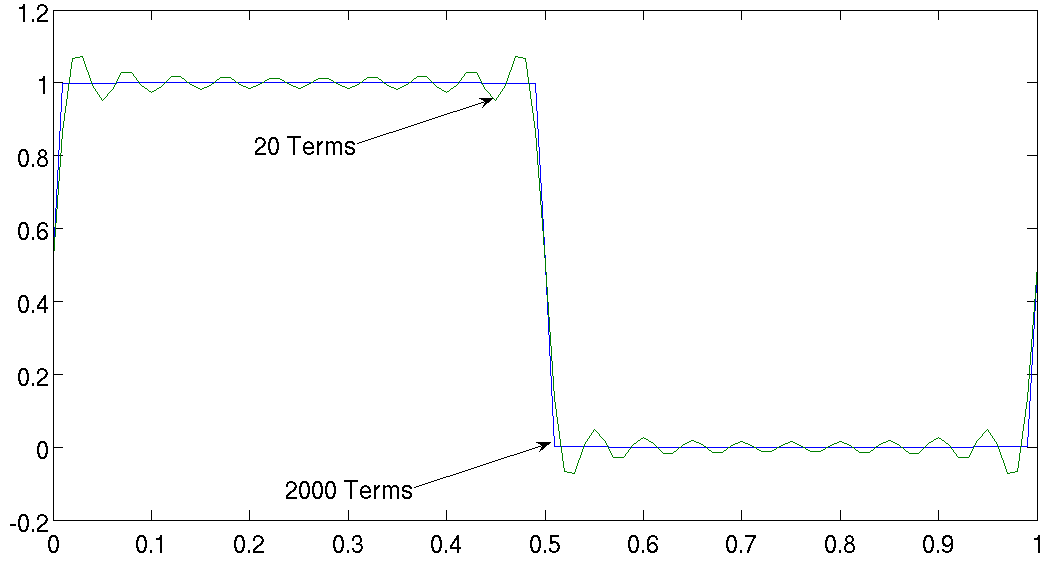
\includegraphics[width=0.75\textwidth]{images/FourierSeries_Cropped.png}
  \end{center}
  \caption[Fourier Series]{\label{figure:FourierSeries}Two Fourier Series fit to a step function, one with 20 terms, and one with 2000 terms. The series with 2000 terms provides much more accuracy and less oscillatory behavior.}
\end{figure}

Several families of functions can be used to approximately represent the surface of the terrain, as well. Fourier series, for instance, can be used, though the oscillatory and symmetric nature of the functions limit their usefulness in this arena. 
Fourier series are particularly popular in that they are infinite series that lend themselves well to \emph{progressive transmission}, a process by which transmission is made more bearable on the receiving end because the terrain can be initially built after receiving just a few coefficients and refined as more are added later. This allows a preview to be seen by the end user before all of the information is available.
Overall, truncated Fourier series are easy to work with, and they are differentiable and continuous. An example of a Fourier Series can be seen in Figure \ref{figure:FourierSeries}.
%  and Equation \ref{equation:FourierSeries}:
% They can be added and combined, a desired trait for a terrain surface. 
It is a simple process to add two or more series, a desired trait for a spatial representation. However, they produce too many local minima and a surface shape that is free of discontinuities, and attempting to model these discontinuities results in poor approximation due to the Gibbs phenomenon in which the function overshoots the target value, creating overcompensating oscillations which are impossible to stamp out, resulting in an overly smooth surface. Also, adjusting a single parameter can affect the entire series, and thus a large section of the terrain, and so local control of the data is not possible. 

B-splines allow for more accurate representations because they can be fit through the known elevation points along the surface to produce an approximation of the shape (Farin \cite{Farin:2001:CSC:501891}, and Faux and Pratt \cite{Faux:1979:CGD:578513}), and allow them to act as local control points. In addition, the connectivity between the curves allows the user another level of control over the shape of the surface. This control is limited, however, in that changing where one curve meets another, and the degree of continuity of the meeting, changes the representation on a non-local level. This also may cause problems at the edge of the terrain. B-spline curves are also smooth and continuous, despite the existence of local control points.

Wavelets, another infinite series representation, are not constrained to a continuous approximation. They can approximate the terrain with arbitrary accuracy as a result, including the local discontinuities. They and Fourier series share the property of progressive transmission. These properties account for the popularity of the wavelet representation. However, they still lack a strong correlation to the physical world, and as such cannot store generation information inherently. 

There are many similar methods in existence. Bertam et al. \cite{Bertram:2003:ASS:769922.769942} present a method for converting 2D point clouds into surfaces by segmenting the points into regions and then creating a quadratic or linear estimation of the points in each region using an adaptive quadtree algorithm.  Nobre et al. \cite{Nobre_Cuartas_Hodnett_Rennó_Rodrigues_Silveira_Waterloo_Saleska_2011} describe a new method for terrain representation that classifies different height ranges by their distance from the drainage outlet, normalized across the entire dataset. 

Each of these surface representations harbors another fundamental flaw in that they have no correlation to real world physics. Because they are only spatial data points (or a approximation, in the case of Fourier series), they do not allow for encoding information regarding the formation of the terrain, and have no connection to the physics (hydraulic erosion) responsible for it.


\section{Volumetric Representations of Terrain}
\label{section:VolumetricRepresentations}

\begin{figure}[t]
    \centering
    \begin{minipage}{0.49\textwidth}
      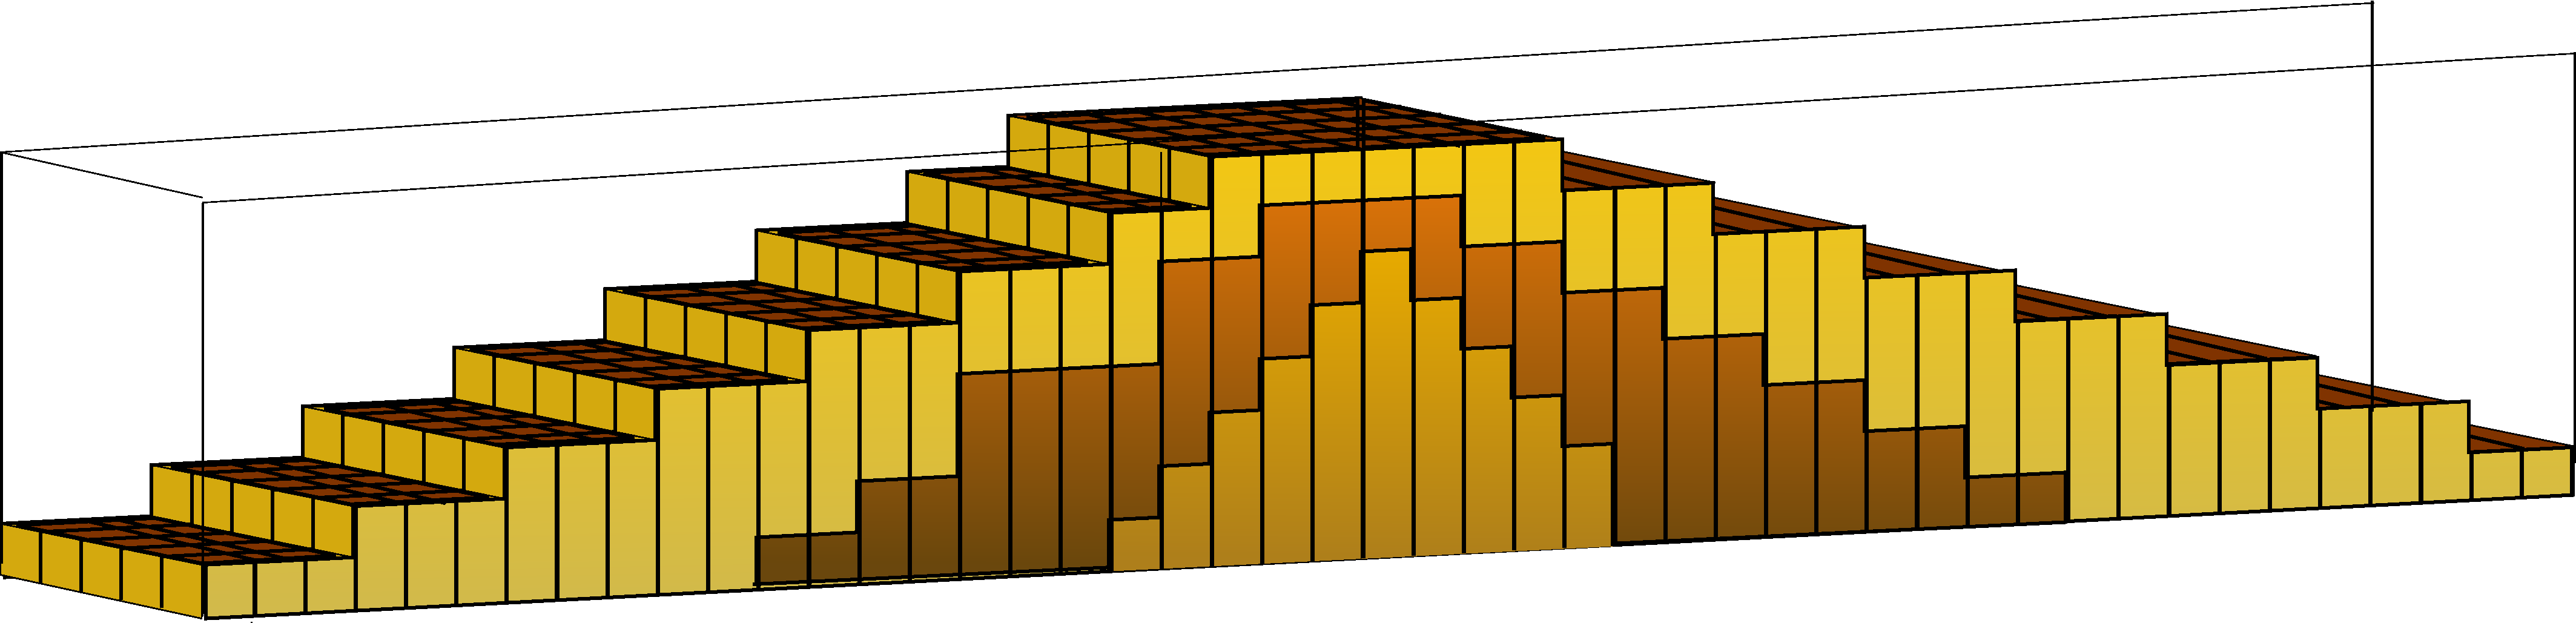
\includegraphics[width=1.0\textwidth, height=0.15\textheight]{images/SHF.pdf} 	 
    \end{minipage}
% 
   \begin{minipage}{0.49\textwidth}
    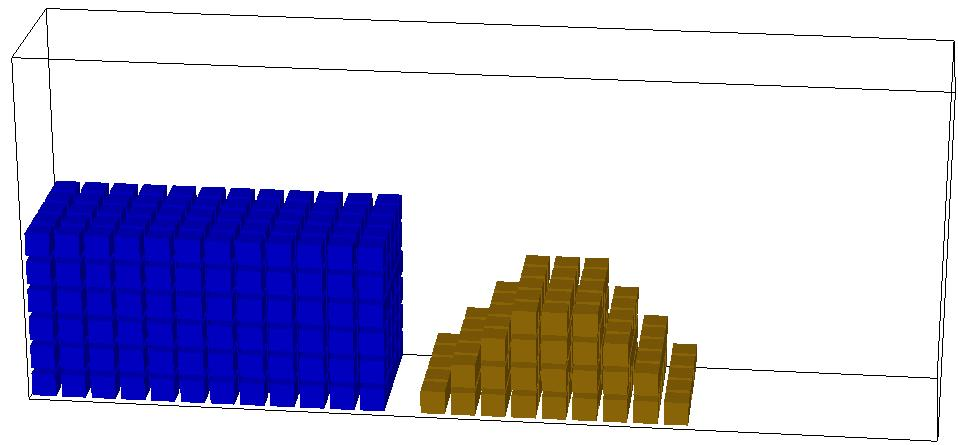
\includegraphics[width=1.0\textwidth]{images/VoxelGrid.jpg}
   \end{minipage}
% 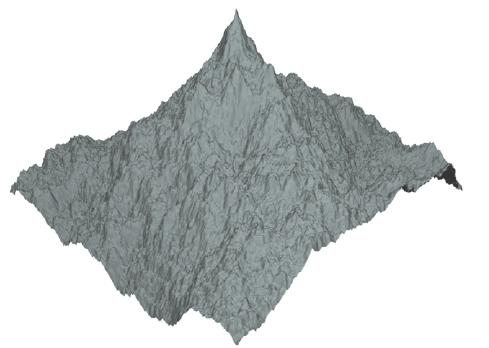
\includegraphics{images/HeightField.jpg} 
% 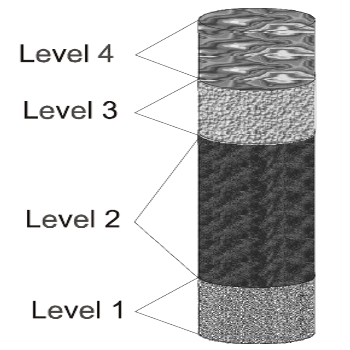
\includegraphics{images/LayeredDataRepresentation.png} 
	\caption[A rendering of volumetric terrain data structures]{(Left) 
% A rendered height field, in which the terrain is discretized into cells, each of which stores a single height. (Center) 
A layered height field, in which every grid space of the height field contains an array of arranged layers.
% similar to a height field except each cell contains an array of layers. 
(Right) A voxel grid, in which the terrain is constructed of cubes of materials, discretized in three dimensions.}
	\label{figure:data_structures}
\end{figure}

Many applications in computer graphics, such as erosion or weathering simulations, can be made more accurate and precise when terrain data is represented volumetrically. 

A voxel based terrain representation allows for immediate coupling with many fluid simulation techniques, as these are often based on a voxel grid (Figure \ref{figure:data_structures}). Fluid simulation (with terrain boundaries) using the Navier-Stokes equations is a straightforward application for a voxel grid, for instance. Voxel-based terrain representations allow for multiple materials, each with its own set of soil parameters, allowing for a more accurate simulation. Voxel grids allow for caves and undercuts as well because it is possible to model air as well as soil and fluid. Because of this, there is no limit to the fluid-soil boundary. Surface data is straightforward to draw from a voxel grid, but more importantly volume information is also inherent in the representation. Voxels also make complex renderings possible. However, voxel grids limit the precision of the terrain model, and the accuracy of the simulation is dependent upon the resolution of the grid in all three dimensions, as opposed to only two dimensions as for a height field. Voxel grids also require a lot of space to store, as well as connectivity information when dealing with soil layers.

Benes et al. \cite{Benes-LayeredDataRep} present a layered height field that combines several advantages of each of height fields and voxel grids. In their structure, the terrain is divided into a two dimensional grid, like a height field, but each grid space contains an array of heights (Figure \ref{figure:data_structures}). This representation allows for several different soil types, and a surface can be easily extracted for visualization and simulation purposes. The precision is arbitrary (to the degree of the computer's limit) because heights are stored as floating point values, which also significantly reduces storage. Most importantly, the layered representation allows for caves and undercuts by representing open air as one of the layers. The layered height field, however, does not allow for dynamic ordering of the layers, so new layers cannot be formed and if a particular soil type does not appear in a grid column then its value has zero depth, wasting space. If a dynamic implementation is used, new layers are added, then the newly added layer must be applied across the entire grid. Because sediment deposition may cause hundreds of layers to be added during a complex erosion simulation, this representation requires significant tuning before it is useful to us.

Some other representations have been used for terrain or similar models. Agarwala et al. \cite{argwala-Volume} present the ``slab'' data structure and use it for surface sculpting of volumetric models. Along the surface of the volume are assigned slabs, or small volumetric grids, that make local changes easier while not affecting the entire volume, thereby not requiring a global update. The slabs allow for updates to be made on a discrete grid structure while maintaining the underlying volumetric information of the rest of the model untouched by changes to the surface. The slabs are stored in quad-trees, allowing for local resolution adjustments as necessary by the level of detail required by a simulation. The authors use the slab data structure in the implementation of a surface sculpting simulation that requires only local updates when the surface is cut away. The authors also present a method for updating the rendering of the slabs by manipulating the display buffers to only update along the line of a stroke by a tool in the simulation. 
% This structure is too detailed for our purposes, but 
The idea of combining the benefits of many representations is an important one.

\section{Hydrography Network}
\label{section:PriorLiteratureChannelNetworkExtraction}

% \fbox{REWORD THESE, AND FIX THE CITATIONS}

An essential characteristic of terrain is its hydrography, consisting of the channel network (also known as its drainage or river network),
because hydraulic erosion is a prime factor in the
formation of terrain geometry.
% , particularly for levee breach events that motivate my work.
Accurate and efficient extraction of these networks
from DEM data has been an area of study for several
decades. It is essential for the analysis and comparison of terrains
as it allows for identification of channels, watersheds, valleys, and
drainage basins, but its challenges stem from the fact that the data
contains no information regarding the behavior of basins.
% 
Because of its importance, the pixels that make up the channels of the terrain's channel network 
are the focus of the placement of the drill operator. A great deal of attention in this 
work is paid to accurately extracting the channels.

%In 1984 
O'Callaghan and Mark \cite{OCALLAGHAN-Extraction} were among the first
to extract a channel network from a DEM, and their method is widely used in practice. 
% For each pixel of the terrain, the direction of the lowest of its eight neighbors is set as the flow direction. The pixels are sorted by elevation, and flow accumulation is calculated. 
Each pixel has its direction of flow calculated by determining the direction of steepest descent among its neighbors, and flow accumulation is calculated.
A threshold is applied to the accumulated flow values, and those pixels that surpass the threshold are considered part of the corresponding channel network.
% 
% This practice is widely
% used in channel network extraction, and finding the best
%ideal 
% threshold for a particular terrain
%to use on a channel network is the basis of our work.
% is one of the specific objectives discussed in this thesis. 
In this method, slight variations in geometry could render a threshold significantly less useful.
% , and so when dealing with sequential data an adaptive threshold is vital. 
Comparing two terrains only makes sense if they have similar channel networks, 
and so identifying optimal thresholds 
% that minimize the difference between the extracted networks 
is an important research question.

In addition, elevation tie-breaking (in the case of an elevation tie between neighboring pixels, such as in basins, determining which pixel is ``lower'' for the purposes of the flow algorithm) and how pits are dealt with continue to be challenging research questions, as the methods used have a surprisingly strong effects on the extracted channel network.

%In 1986, 
L. Band \cite{band86} describes a method for extending O'Callaghan and
Mark's work to identify channel watersheds by grouping pixels that
flow into the same channel. To minimize the need for tie-breaking procedures, grouped pixels are treated as a single pixel.
% Once grouped, they can act as a single pixel and can accumulate flow as one, thus minimizing the need for tie breaking. 
However, this does not solve the problem of flat basins completely.
%In 1997, 
Yang et al. \cite{YANG-geomorphic} describe the effect various
thresholds have on two widely used watershed analysis tools, the {\em
  width function} and the {\em area function}, finding that at low
thresholds the two measures are similar but vary greatly as thresholds
increase and channel networks shrink. 
%In 1993, 
Montgomery and Foufoula \cite{MONTGOMERY-1993} present a
comparison between 
two channel network calculation models, the constant threshold and the slope-dependent models.
% the constant threshold and slope-dependent models
% for calculating channel networks, presenting 
They find that each
method appears valid in certain instances. They also describe a method
for identifying channel heads as a means for extracting channels.

Other methods for channel network extraction have required additional
input. Turcotte et
al. \cite{Turcotte_Fortin_Rousseau_Massicotte_Villeneuve_2001}
introduce the {\em Digital River and Lake Network}, which is required
as input in addition to a DEM. This allows for the handling of lakes
in the terrain, a source of frustration for previous methods because
of the difficulty of tie-breaking procedures.

%  and the lake of flow volume. 
Some methods have foregone flow calculation entirely and
depended upon the geometry of the terrain surface exclusively, such as
Lashermes et al. \cite{Bruno2007}, who present a method for
extracting valleys and hills from a terrain using wavelet filtering on
high resolution DEMs.  Still other methods have attempted to define
characteristics on the terrain. Kramer and
Marder~\cite{PhysRevLett.68.205} use a shallow water simulation to
model the flow of water over the terrain, measuring the formation of
channels with the area and width functions. Similarly, Soille et
al.~\cite{Soille_carvingand} overcome the tie-breaking dilemma in
network extraction by running a flooding simulation to create a path
through pits in the terrain. However, in both of these methods computation
costs make analysis of large terrains difficult.


\section{Terrain Data Compression}
\label{section:TerrainDataCompression}

Terrain data compression is an obvious yet vital application of novel terrain representations. Many representations are specifically designed to be easily compressed, while other schemes take advantage of the characteristics of the more popular representations. The characteristics of terrain that compression schemes should work to retain go beyond simple height values. While it is hard to be absolutely sure of the accurate hydrography data given a terrain dataset (which contains errors due to data collection itself), schemes that ignore this property can easily compound error in what is a critical characteristic of the terrain surface. For this reason, research into compression schemes is varied and extensive.

There are two types of compression: \textit{lossy} and \textit{lossless}. Lossy compression sacrifices some data for a higher compression ratio, whereas no data is lost due to lossless compression. \textit{Near-lossless} compression refers to a scheme that allows the user to bound the error of the regenerated data, meaning that it can be lossless if the user elects to have the bound on the error be 0\%.

\subsection{Compressing Terrain Features}

One of the primary methods for compression is to select the most ``important'' elements of the data and store only them. Pedrini \cite{conf/wscg/Pedrini01} presents a method for building a terrain surface from a set of data points. It alternates between refinement and decimation steps, meaning that a set of points is selected to represent the surface, and then a set of less useful ones are removed from the chosen set, and the process is repeated until a global error threshold is met. Dyn et al. \cite{Dyn02adaptivethinning} present a method for thinning a dataset based on the error present in the triangulation of the points, which entails removing points one-by-one and recalculating the error until a global threshold is met. The algorithm presented works with several triangulation and error calculation techniques. Kolar \cite{1e218e70004511dab4d5000ea68e967b} presents a method for building a level-of-detail hierarchy of triangle vertices using the idea of ``mass points'', or vertices that are assigned to levels in the hierarchy based on the frequency of the terrain around them. 

Similarly, Xie et al. \cite{Xie_approximatingterrain} present the ODETLAP algorithm, which treats a matrix of elevation values (with holes) as an overdetermined Laplacian system with equations for each known elevation value. This allows for a selective compression scheme since an incomplete surface can be rebuilt using ODETLAP, and so only the most ``important'' points are stored. 
This method is also presented by Inanc \cite{inanc-phd}. In his work, Inanc presents the ODETCOM system, which obtains near-lossless 
% (lossy compression whose error is user-bounded) 
compression with good results. Like ODETLAP, ODETCOM creates and overdetermined system of equations using a predictor model. The predictor is based on a template whose size is variable depending upon a desired accuracy threshold, creating a near-lossless scheme.

Pradhan et al. \cite{Pradhan_gisterrain} present a method of compression terrain data that uses a Delaunay triangulation, and a "lifting technique" to compress. During the lifting, each triangle is divided into smaller triangles, allowing each level of the compression to be written as its own wavelet equation, which is then encoded. Along those lines, Kim et al. \cite{Kim_ageometric} present an algorithm for compressing Delaunay triangulations of a series of 2.5D points (that describe a surface). The algorithm revolves around finding both the Delaunay triangulation and any other single triangulation, and defining the ex-or function that finds the set of vertices and edges not in the intersection of both triangulations.
% , achieving good results.
%  The paper introduces a series of theorems about the comparison of triangulations and subgraphs of said triangulations.

\subsection{Image Compression}
\label{subsection:ImageCompression}

Because height field 
% and TIN 
representations of terrain are isometric to greyscale image data, image compression techniques are often used to compress terrains. Grazzini and Chrysoulakis \cite{Grazzini05n.:extraction} take advantage of this characteristic by noting that traditional features of terrain, such as slope, aspect, and curvature, are not scale invariant, and thus do not fit the needs of all representations. And so they present a terrain feature extraction method for greyscale images using a multifractal representation of image data. 

Image compression techniques ignore many of the features found on terrain, and do not take advantage of the characteristics of terrain that many terrain-specific compression schemes do. However, from a purely statistical standpoint,  they are more successful in general with regard to compression ratios. There are many families of image compression schemes, the most widely used being JPEG and PNG.
% , and medical image compressions.

JPEG (named after the group that created it: Joint Photographic Experts Group) \cite{Penn92}
is the industry standard for lossy image compression, and consists of a series of steps to transform, downsample, and quantize image information before encoding. 
The algorithm divides the image into a series of smaller blocks (8 x 8 groups of pixels) that it treats as matrices that are transformed to the frequency domain via the Discrete Cosine Transform. The result of this transform can be truncated and encoded, which provides for the compression.
% The process works by identifying blocks of pixels with similar chrominance and downsampling to reduce redundancy. The scheme works well in a terrain domain because neighboring pixels often share similar elevations, or intensity values in image space, which allows for large blocks to be identified and encoded.
JPEG compression often obtains 20:1 compression ratios with no noticeable degradation to quality. This serves as a good baseline comparison for terrain compression schemes.
% 
A variation on JPEG, called JPEG-2000 \cite{Taubman:2001:JIC:559856}, is a lossless scheme that takes advantage of wavelets to compress image data.

PNG (Portable Network Graphics) image compression \cite{316738} creates a string of sequential differences between color values of the pixels of the image. Storing the first pixel value and then a series of distances creates a situation in which homogeneous sections (with several 0s in a row) can be compressed effectively with run length encoding, or other similar schemes. PNG compression is lossless, but like many lossless schemes can be converted to a lossy scheme by sacrificing some accuracy by sampling, obtaining a better compression ratio.

The JBIG compression scheme \cite{Kyrki99jbigimage} was designed for binary images and uses IBM's Q-Coder arithmetic coder to encode each pixel, a function of its immediate neighborhood. A greyscale (or even color) image can be compressed by acting on a single bit plane at a time (i.e., treat an 8-bit-per-pixel greyscale image as 8 separate binary images). 

Dozens of other compression schemes exist for images. Some are optimized for greyscale images, some for color, and some specialize in specific kind of images, such as medical images (Zukoski et al.\cite{Zukoski:2006:NAM:1356588.1356594}, Raj and Venkateswarlu \cite{Raj:2007:NAM:1335117.1335447}, for example).
% 
It is difficult to best standard image compression schemes with regard to compression ratio. The primary goal of terrain data compression is meeting an accuracy threshold with as high a compression ratio as possible. A lossy image compression scheme may result in small elevation errors that exacerbate the error in the hydrography of the regenerated terrain surface. As such, they are not necessarily ideal, despite their superior compression ratios. 

% \fbox{FINISH THIS SECTION WITH A MORE EXAMPLES}


% \section{Shape Analysis Techniques}
% \label{section:ShapeAnalysisTechniques}
% 
% In order to judge the accuracy of terrain representations and compression schemes (or any application in which there is an attempt to match spatial data),
% % such as a height field), 
% a method for determining a ``distance'', or measure of dissimilarity, between two 
% % terrain
% datasets is used. One way in which this is accomplished is through shape analysis.
% % \subsubsection{Using Shape Analysis}
% 
% Shape analysis has been studied in computer graphics and computer vision
% for decades, most often used in shape
% matching and pattern recognition. Shape matching is the process of choosing,
%  from a set of possible partners,
%  the closest to a given shape, while pattern recognition is a computer vision
% problem involving picking out examples of a given shape in an image or scene. 
% Shape matching relies on difference metrics, measures of the dissimilarity
% between two shapes. The smaller the dissimilarity, the closer the two
% shapes are to one another.
% 
% Treating terrains and their associated channel networks as shapes is a
% method for comparison from which distance metrics arise naturally. Fundamentally
% the goal is to be able to compare the shapes of the extracted channel networks.
% % that are extracted from terrain data. 
% 
% Often, shape dissimilarity metrics
% are used as bases for finding the correlation between shapes, if one
% exists.  Belongie et al.~\cite{belongie-ShapeContexts} present the
% idea of ``Shape Contexts'', in which a two dimensional shape is
% described by the angle to the X-axis of the tangent of every point along the border of the shape. In this instance, the X$_{2}$ metric can be used as the
% dissimilarity measure between the shapes. An
% extension~\cite{Belongie:2002:SMO:628328.628792}
% to this idea broadens
% the criteria for the shape context by basing its measure on the shape's angle relative to the
% tangent along the shape border instead of the X-axis,
%  making the shape
% context operation invariant under rotation.
% 
% Shape comparison was later applied to three dimensions 
% by Osada~\cite{Osada-ShapeDistributions}, who presents the idea of
% representing three dimensional shapes as a probability
% distribution. Given any shape distribution function (such as the
% \emph{D2} function, a measure of Euclidean distance between two random
% points on the shape surface), the authors build a probability distribution
% function of the shape by selecting random points along the
% surface. These probability distributions can then be compared and
% analyzed by any known means.
% 
% Roy et al.~\cite{Roy04meshcomparison} provide a metric for comparing
% triangle meshes. For each sampled point on the first mesh and a given
% shape attribute, the method finds the closest point of the same
% attribute in the comparison mesh. Geiger et
% al.~\cite{Geiger:2003:RSS:628334.628872} find the Shape Axis tree
% (first presented in Luh and Geifer~\cite{Luh-791256}) and use an
% optimization function to find self-similarity in shapes. They identify
% the best match between two spline curves, one representing the
% parameterized shape and the other representing the shape parameterized
% in reverse. 
% Gal et al.~\cite{10.1109/TVCG.2007.45} present a new
% pose-oblivious shape signature function that defines the overall
% topography of a shape. This is achieved through use of the local
% diameter function and the centricity function, in which the distance between the mesh and a ray
% shot perpendicular to the normal at a point along the mesh is
% measured.  The second function is a measure
% of the average geodesic distance from a point on the mesh to every
% other point on the mesh.  
% Mademlis et
% al.~\cite{Mademlis-ShapeRetrieval} describe a method for shape
% retrieval by matching shapes with those in a database. The algorithm
% segments the shapes, and builds a probability matrix for each segment
% of each shaping, defining the probability that segment $i$ in one shape
% matches segment $j$ in the other. 
% By applying a metric to this
% probability matrix, they determine the likelihood that the two shapes
% match.
% 
% Shape analysis has also been used for animation and deformations.
% M\"ueller et al.~\cite{Muller:2005:MDB:1186822.1073216} present a
% simulation of deformable objects by creating a \emph{goal state} for
% the mesh and minimizing the total energy required to deform the mesh
% to the goal state. Correspondences between points on the current and
% goal states are found through shape matching algorithms. Huang et
% al.~\cite{10.1109/3DIM.2007.8} compare the performance of four
% well-known shape dissimilarity metrics, testing frames in three
% different human animations.
% 
% 
% 
% % These methods provide a useful basis for comparing two meshes,
% % including height fields. However, my needs revolve around specific
% % aspects of the terrains, namely the channel network. To the best of
% % my knowledge, no shape analysis tools have been specifically applied
% % to height field data in computer science literature. In my work, we
% % use variations on the Hausdorff distance, as well as direct pixel to
% % pixel comparisons, to determine the distance between two channel
% % networks, a vital process for terrain comparison and failure
% % diagnosis.



\section{Summary of Prior Art in Terrain Modeling}

Existing spatial representations of terrain data include height fields, TINs, 
and splines. These spatial models fail to accurately represent complex surface features, such as 
caves and cliff faces, which introduce surface discontinuities. 
% 
Volumetric representations, such as voxel grids, are capable of representing
these features, but with too large of a memory footprint to be practically
useful in many GIS applications. 
% 
In addition, none of these representations maintain ties to the hydraulic
erosion responsible for the formation of the terrain, ignoring the hydrography
of the surface.
% 

Hydrographically valid terrains are important for a variety of GIS applications, including many that require the extraction of an accurate and suitable channel network. These include path planning, dam siting, and observer siting algorithms, among others. GIS lacks a procedural representation of terrain whose formation guarantees hydrographic validity by removing local minima and allowing the encoding of complex terrain features.
Until such a representation exists, there is little need to work toward more accurate and robust data collection procedures.

Many data compression techniques, such as feature or image compression, ignore the need to maintain hydrographically valid terrain data, as well. These schemes, while accomplishing substantial compression ratios, fail to maintain important features, and are not tied to any specific representation or formation procedure.

% The surface's hydrography network, or channel network, can be extracted from the surface
% using a variety of methods. Some require pre-processing the terrain, such as filling in 
% pits. Others find the least-cost path from a pixel to the edge of the terrain. 

Moving toward more accurate terrain data collection and storage requires
a representation of the terrain surface that is capable of overcoming these
shortcomings. 
% 
The drill operator, presented in Chapter \ref{chapter:DrillOperator},
has been designed with this goal in mind.










\chapter{The Drill Operator}
\label{chapter:DrillOperator} 

As discussed in Section \ref{section:SurfaceRepresentations}, common representations of terrain data have several shortcomings that limit their utility and accuracy in many applications. Simply storing spatial terrain data, with no regard for the physical process of the generation of the terrain, perpetuates these shortcomings by limiting how closely these representations can mimic real-world terrain and the formations found within. The physics of terrain formation should not be an afterthought when encoding a surface, but instead the focus of the representation.

With this in mind, this chapter presents the \emph{drill operator}, a mathematical operation that carves out terrain by ``drilling'' down into it along the segments (individual branches of the tree structure) of its extracted channel network, changing its shape to fit the channel's profile at each position along the channel's length. 
This work is directly influenced by the work of Franklin et al. \cite{wrf-autocarto-2006}, in which the authors introduce the idea of ``scooping'' the terrain. This idea of representing the terrain with a series of mathematical operations was the main influence of the drill operator.
% Also provided is the results of a series of accuracy tests on a real terrain dataset, providing evidence of the utility of the drill operator.

\section{The Terrain's Hydrography}
\label{section:ChannelNetworkExtraction}

\begin{figure}[t]
\begin{center}
  \begin{minipage}{0.49\linewidth} 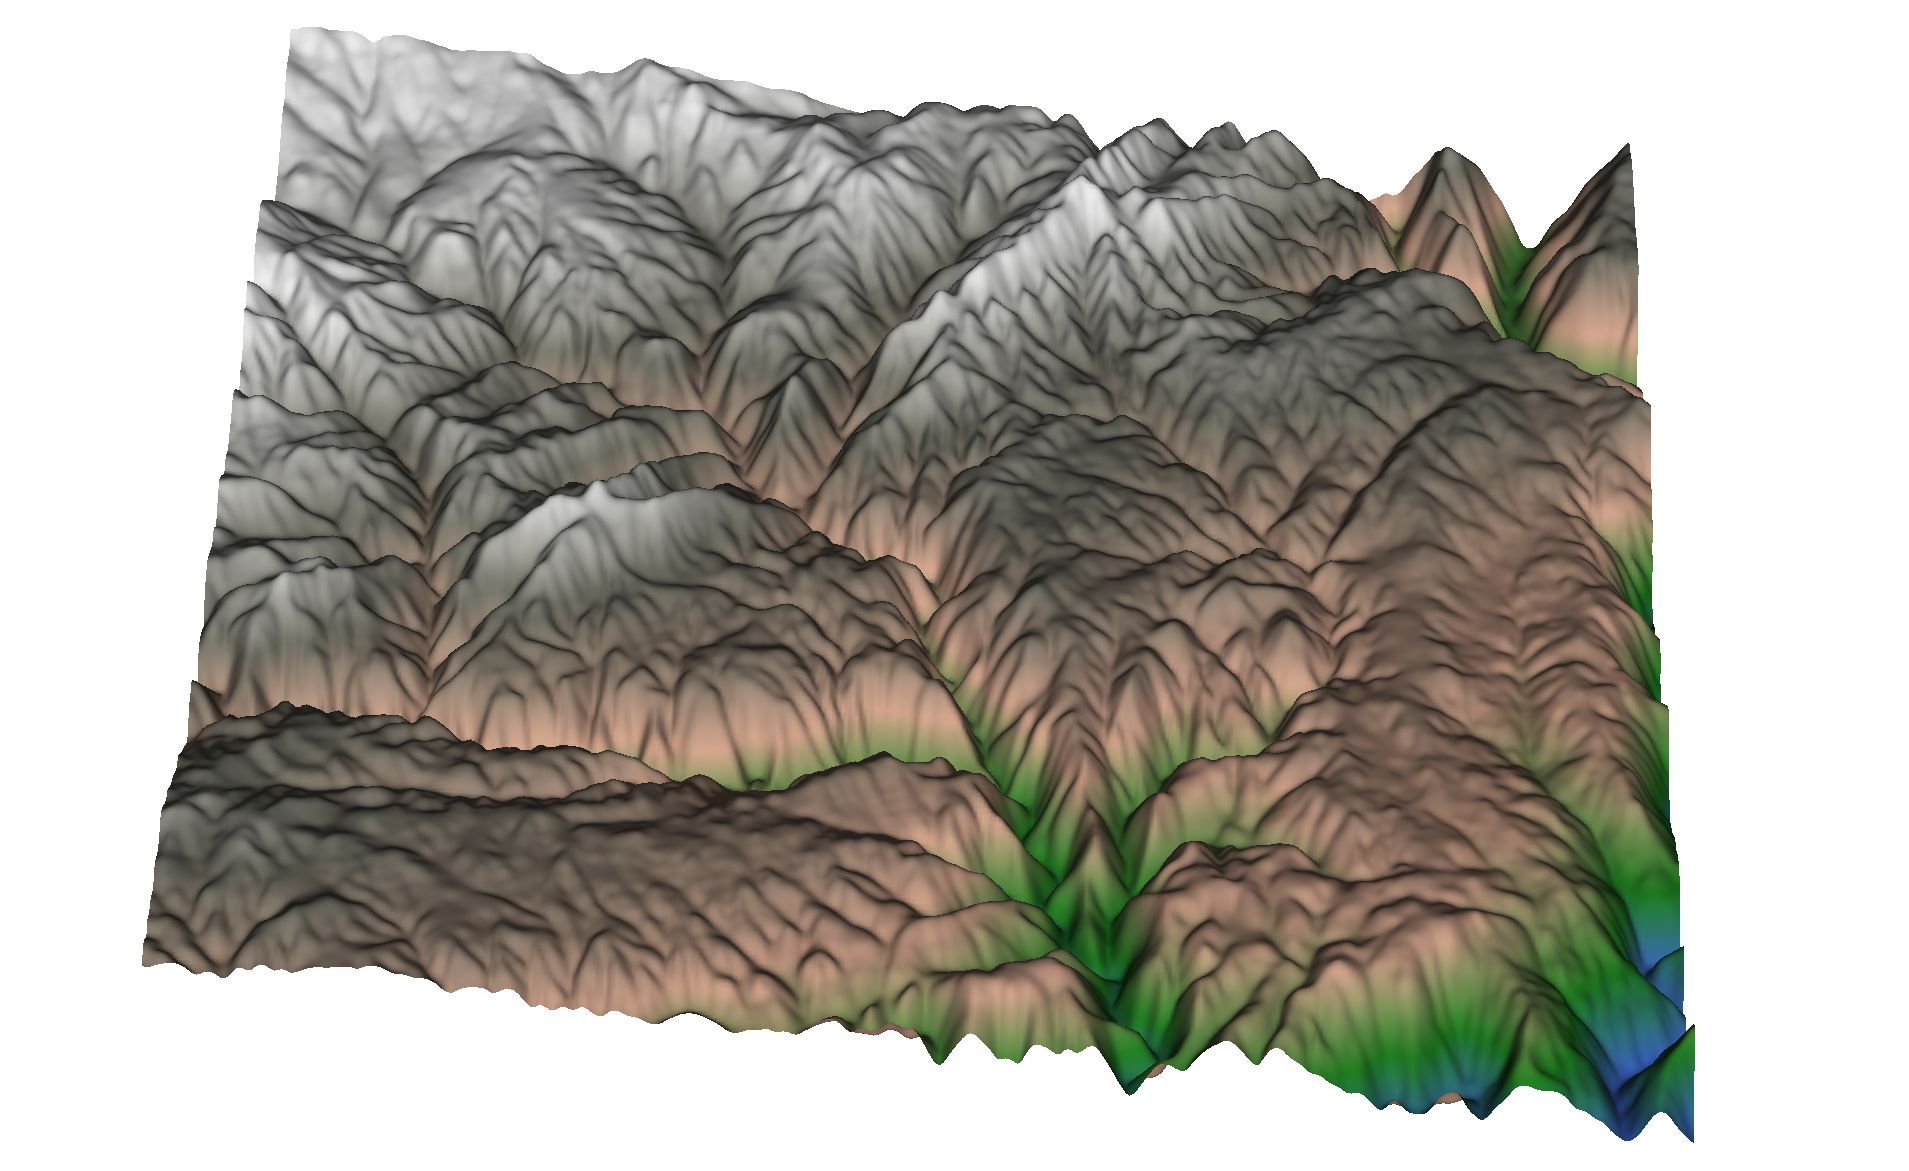
\includegraphics[width=0.99\linewidth]{images/mtn2_original.jpg} \\ \centering Original dataset \end{minipage}
  \begin{minipage}{0.49\linewidth} 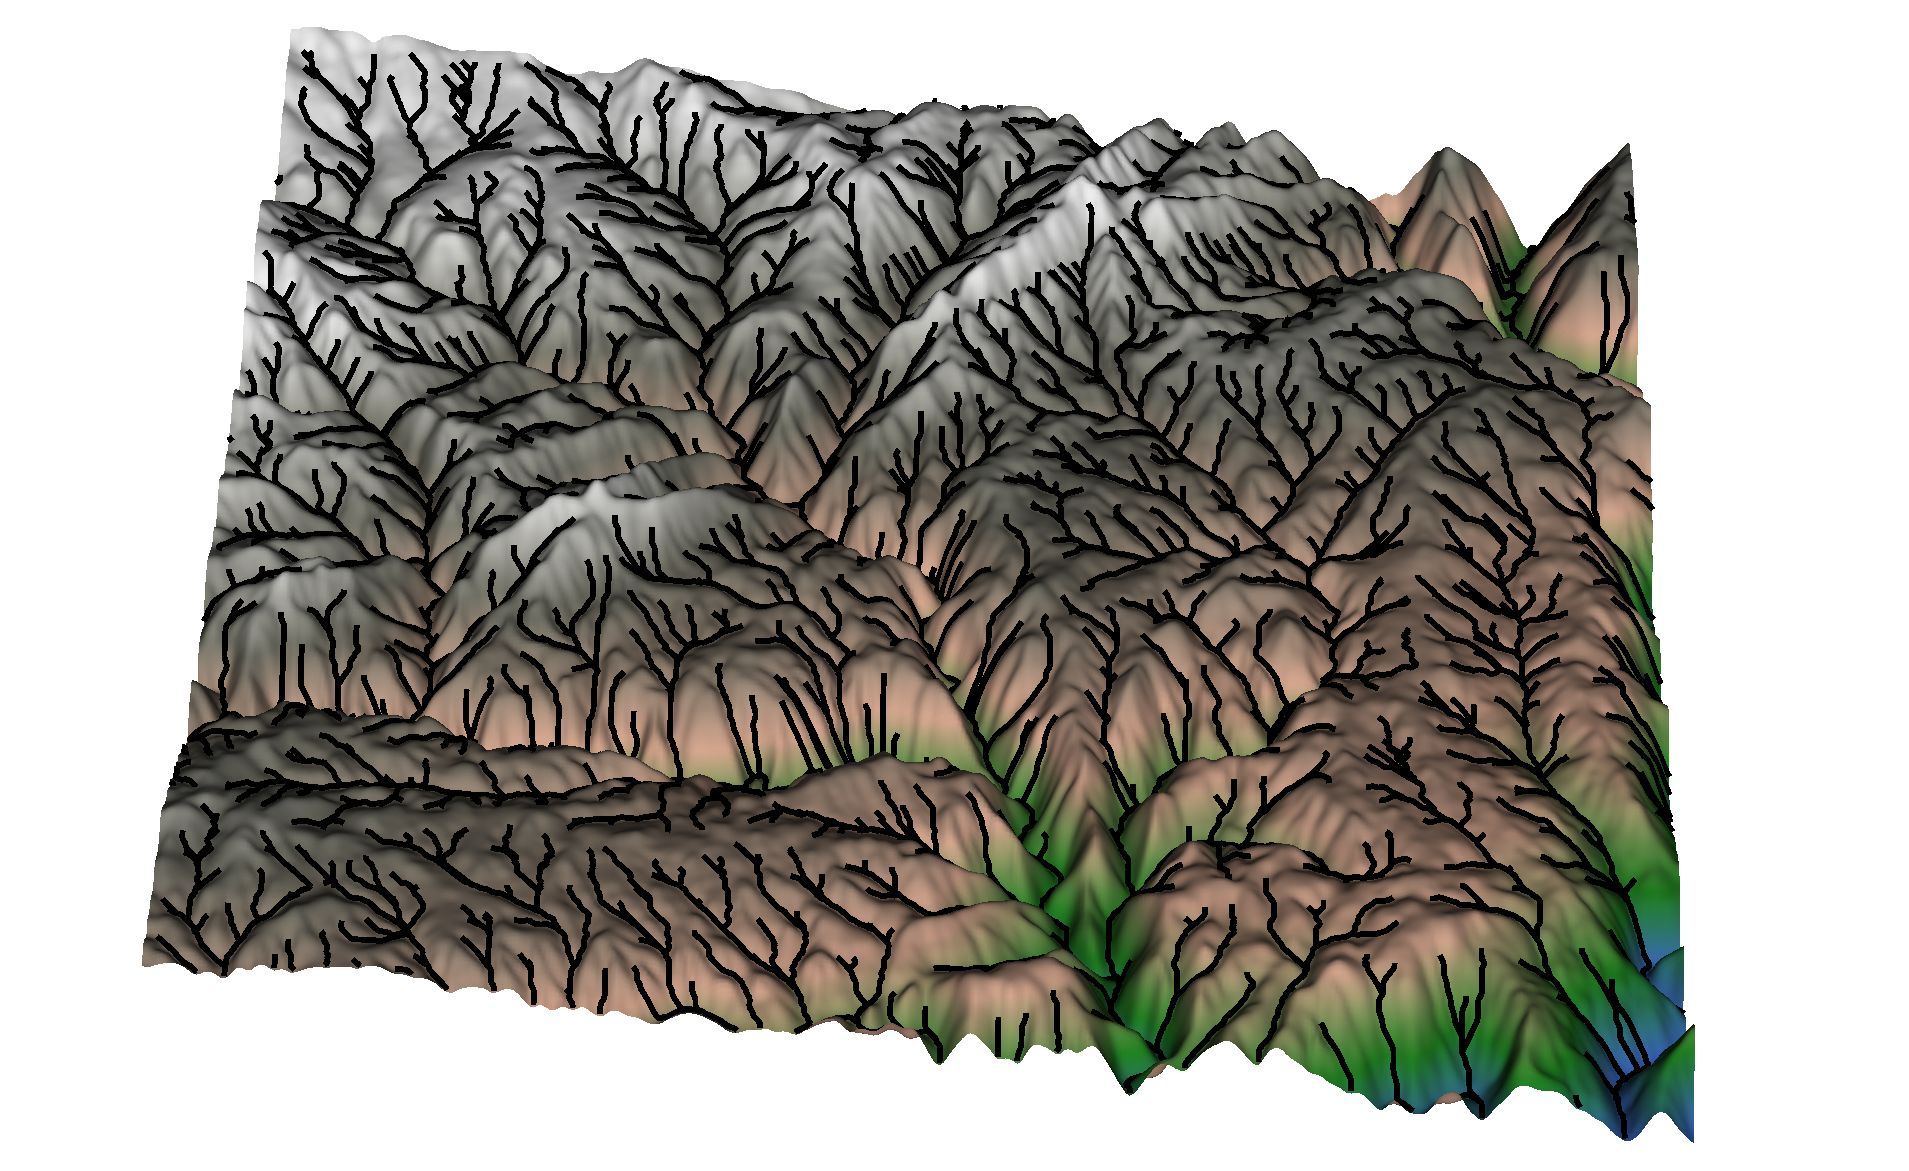
\includegraphics[width=0.99\linewidth]{images/mtn2_T25.jpg} \\ \centering $\tau = 25$ \end{minipage} \\
  \begin{minipage}{0.49\linewidth} 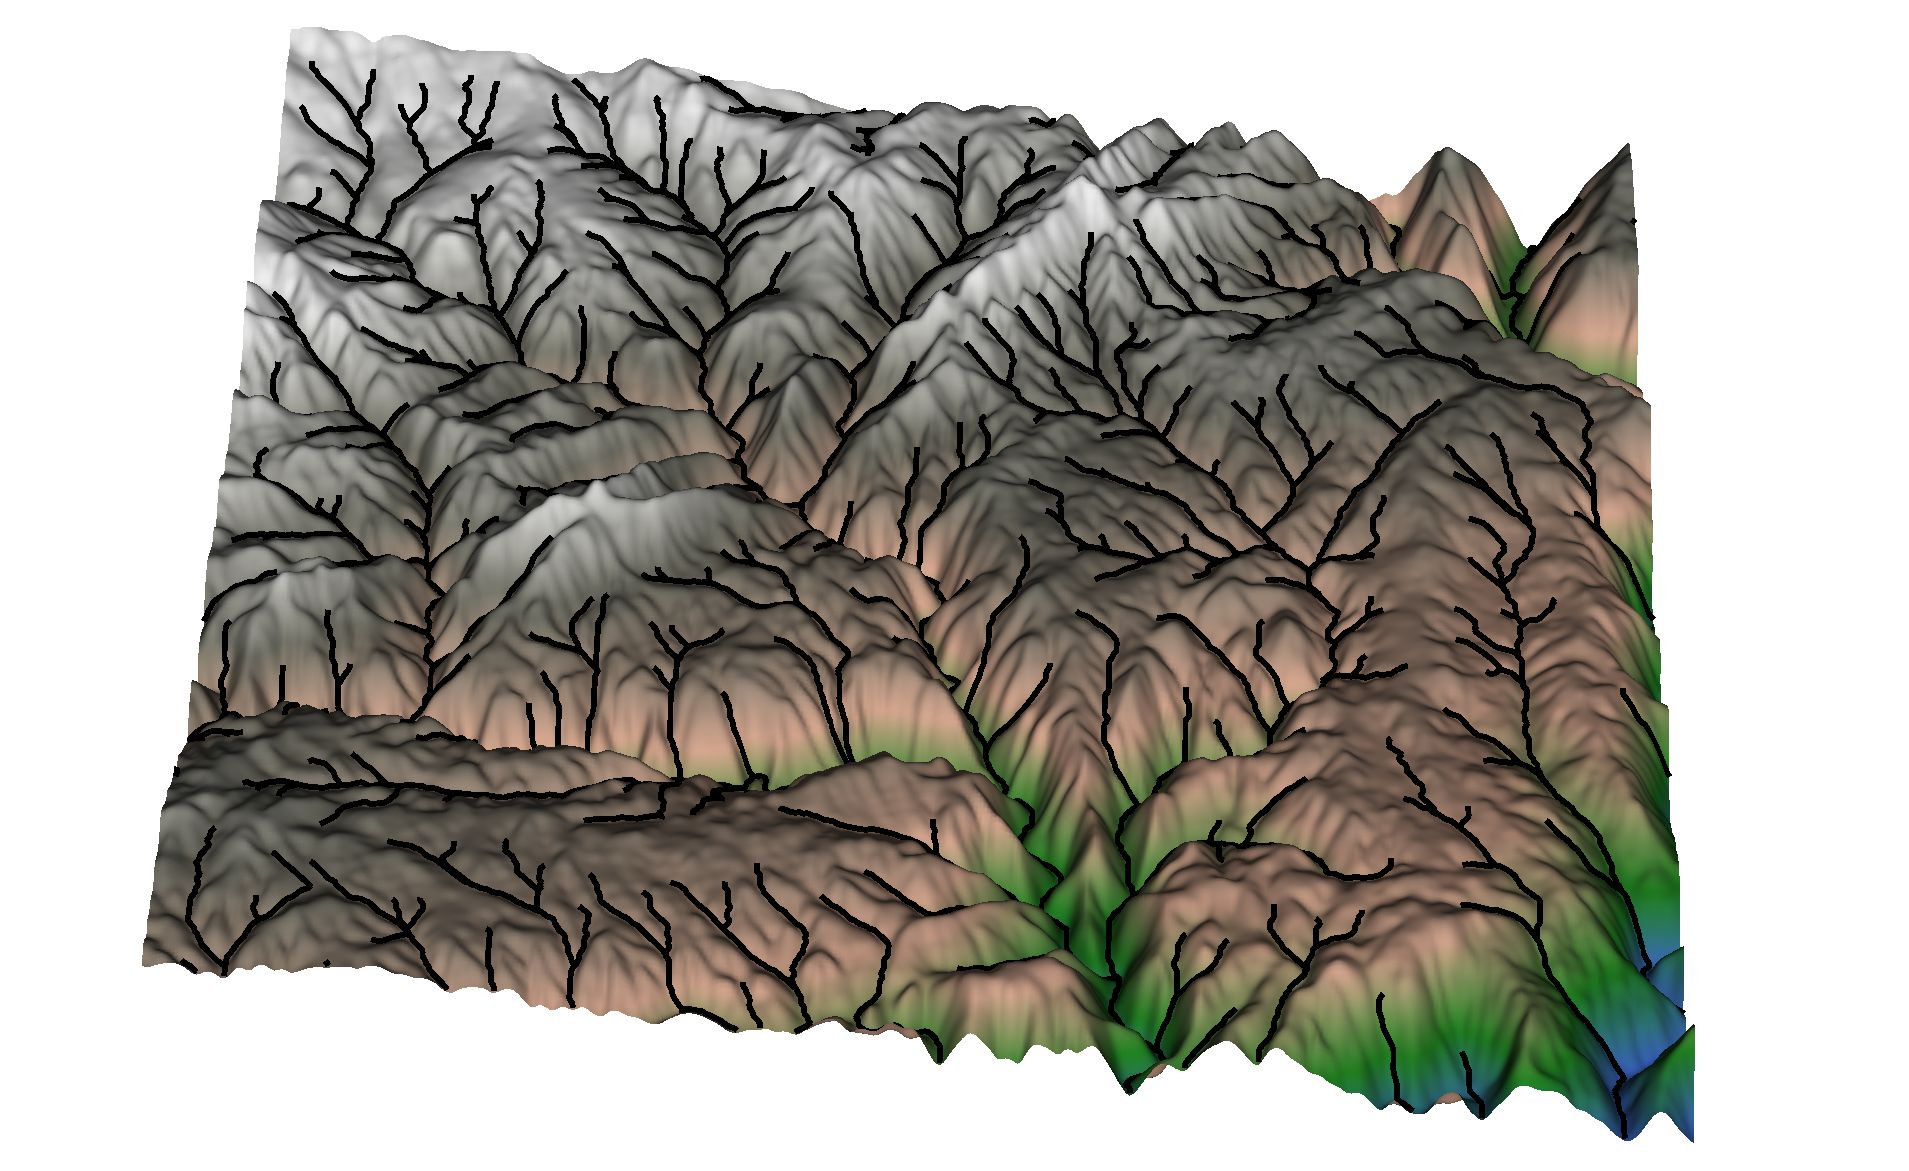
\includegraphics[width=0.99\linewidth]{images/mtn2_T100.jpg}\\ \centering $\tau = 100$ \end{minipage}
  \begin{minipage}{0.49\linewidth} 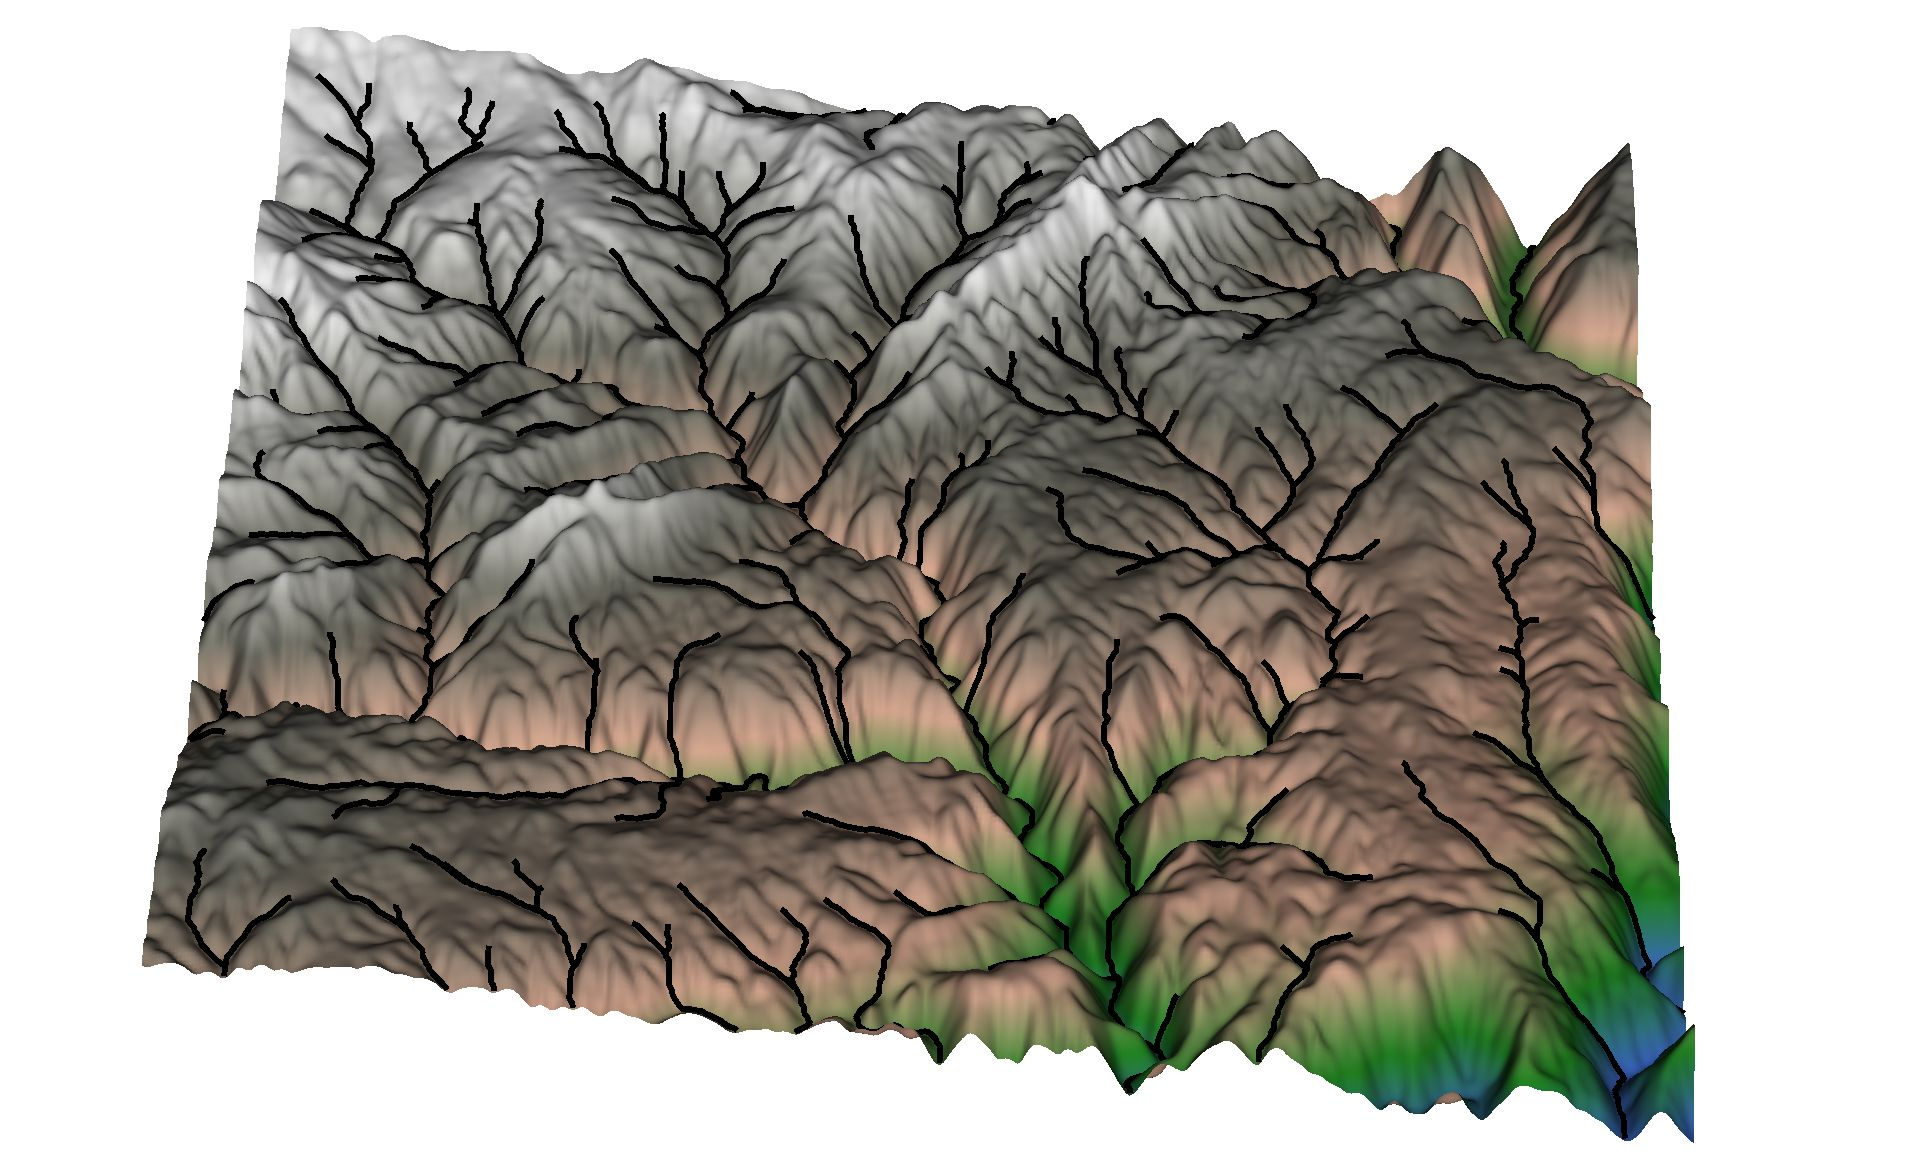
\includegraphics[width=0.99\linewidth]{images/mtn2_T200.jpg}\\ \centering $\tau = 200$ \end{minipage}
\end{center}
\caption[Four mountain datasets with extracted channel networks]{\label{figure:mtn2_original} Four depictions of a $400 \times 400$ mountainous dataset (MTN2 from Figure \ref{figure:SixDatasets}) visualized as a height field of pixels. Color indicates elevation, where white is the highest elevation, followed by brown, then green, and finally blue, which indicates the lowest elevation. Below each data set is the threshold value used to extract the channel network depicted on the surface of each terrain. Notice the difference in the densities of the channel pixels as the threshold increases.}
\end{figure}

For this and many other applications presented in this thesis, it is necessary to determine which pixels of the terrain are deemed to be ``important''. That is, which pixels are part of the terrain formations that are of consequence when terrain is represented, compressed, and analyzed. These pixels are those in the terrain's channel network, and popular methods for their extraction were discussed in Section \ref{section:PriorLiteratureChannelNetworkExtraction}. Most channel network extraction methods determine the flow direction matrix, and then use the flow accumulation algorithm presented by O'Callaghan and Mark \cite{OCALLAGHAN-Extraction} to extract the pixels of the channel network. In this work, the threshold $\tau$ applied to the flow accumulation matrix determined by this method can also be based on a user defined percentage value $r$, which represents a percentage of pixels of the terrain to be included in the channel network.
An example of the effect various values of $\tau$ can have on the channel network can be seen in Figure \ref{figure:mtn2_original}.
The method used for determining flow direction in this thesis was presented by Metz et al. \cite{hess-15-667-2011} in 2011, and is the algorithm currently used in the \textit{GRASS} software.

\subsection{Extracting the Channel Network}

Given a height field $T$ made up of $n$ pixels $\textbf{p}_i$ with elevation values, the algorithm uses a bottom-up elevation-based priority approach to determine flow direction. It uses a priority queue $Q$ which holds pixels prioritized by elevation first and order-of-input into the queue second. 

First, the set of possible flow outlet points are determined. These points are generally the pixels along the border (as in this work), but can also be any sinks identified within the terrain. These pixels are added to $Q$. Then each pixel of highest priority (lowest elevation) is processed in order until $Q$ is empty. For each pixel $\textbf{p}_i$, all neighbors of $\textbf{p}_i$ that have not yet been processed (placed in $Q$) have their flow directions set toward $\textbf{p}_i$, and are added to $Q$. After each $\textbf{p}_i$ has been processed in this manner (meaning $Q$ is empty), the flow direction matrix will be generated.

% In order to extract the channel network once the flow direction matrix is calculated, a threshold $\tau$ is applied to the pixels 

This method has several advantages over that presented by O'Callaghan and Mark. First, there is no need to pre-process the terrain to take care of pits and basins. 
Normally, without complex additional rules added to the algorithm, pits halt flow direction calculation because no neighbor has a lower elevation. 
Basins cause problems because they are created by many neighboring pixels with the same elevation values, so tie-breaking processes are necessary and add a level of complexity to the algorithm.
Since this method ignores neighbor heights and only takes advantage of the fact that the neighboring pixels are adjacent to the current, pits and basins are no longer an issue. Each pixel simply flows in the direction of the outlet it is ``closest'' to, elevation-wise. 
% While this is not always the case, no method yet presented in the area produces a flow network guaranteed to be correct all of the time, nor is such a request feasible.

Secondly, the method is fast ($O\left(n \log{n}\right)$), which is based on the speed of the priority queue implementation, and so advances in priority queue implementation lead directly to speedups for this algorithm. Thirdly, the algorithm provides a pixel list ordered from lowest elevation to highest, which is saved and used in several other portions of this work, saving a great deal of time in the future. The fact that pixels are processed in a bottom-up order allows for future algorithms to be optimized for this ordering. 

\subsection{Choosing a Flow Threshold}
\label{section:ChoosingAFlowThreshold}

% As described in Section \ref{section:ChannelNetworkExtraction}, to extract the channel network $N_{\tau}$ from a terrain $T$, a threshold $\tau$ is applied to $T$'s flow accumulation matrix $flowAccum_{T}$. 
% This section describes a method of determining an optimal threshold to apply to a pair of terrains to minimize the distance between their channel networks. 

\begin{figure*}[t]
\centering
\begin{minipage}[b]{0.45\linewidth}
\begin{center}
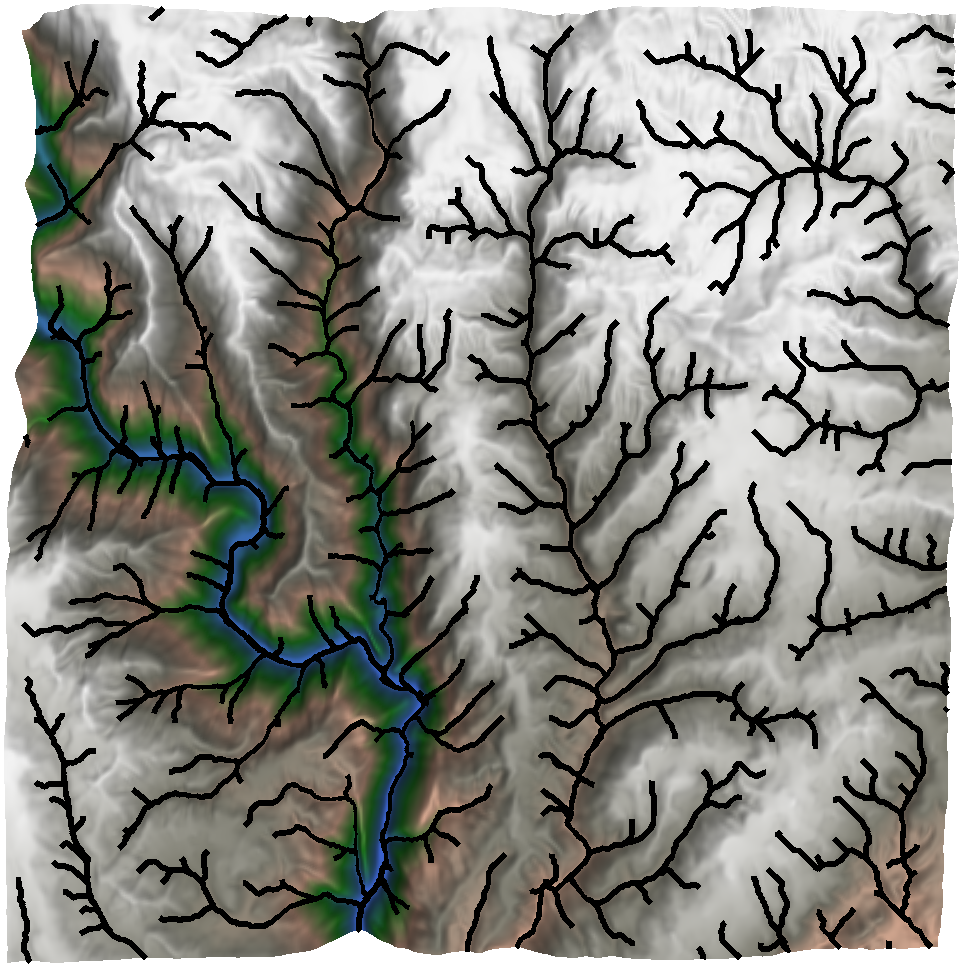
\includegraphics[width=\linewidth]{images/ChannelNetworkWithoutWeights_160_mtn3.png}
\end{center}
\end{minipage}
\begin{minipage}[b]{0.45\linewidth}
\begin{center}
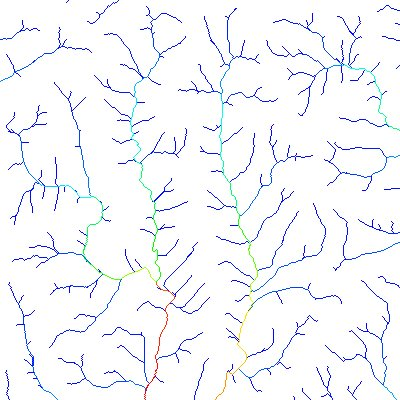
\includegraphics[width=\linewidth]{images/FlowField_mtn3_WithoutWeight.jpg}
\end{center}
\end{minipage}
\caption[An extracted channel network on MTN3 with a global threshold.]{\label{figure:ChannelNetwork_GlobalThreshold} An extracted channel network on MTN3 using one global flow threshold of 160 units of flow. Left: A bird's-eye view of the extracted channel network, with the pixels whose flow values exceed 160 units of flow shown in black. Right: A visualization of the flow accumulation matrix (after thresholding). Red indicates maximum flow, and blue indicates minimum flow. }
\end{figure*}



Traditionally, a single global threshold $\tau$ is applied to $flowAccum_{T}$,
% the flow accumulation matrix, 
and any pixels whose flow value exceeds the threshold are considered to be part of the channel network $N_{\tau}$. An example of an extracted channel network on MTN3 can be seen in figure \ref{figure:ChannelNetwork_GlobalThreshold}, in which channels are drawn in black on the terrain. The goal of any channel network extraction algorithm is to closely match the ``blue-line'' standard, or the accepted channels that a hydrologist studying the terrain in question would identify. In many cases, a single global threshold does an acceptable job identifying the intuitive placement of channels. However, one major drawback to using a single threshold is that the procedure is biased towards lower elevations, as flow accumulates in a top down fashion. Because there is less water available at the higher elevations, this creates a bias.

There have been several attempts to rectify this, such as use of other criterion for thresholding. Tarboton et al. \cite{Tarboton-OnExtraction} suggest using drainage density, constant drop procedures, or slope scaling procedures to properly weight pixels when deciding which should be included in the channel network. In this thesis, a weighting scheme is applied that assigns a different weight to the threshold for each pixel. The weight ($w_{thresh}$) is calculated as follows:

\begin{align}
  heightP & = \frac{ \textbf{p}_{z} - min\left(T\right) }{ max\left(T\right) - min\left(T\right) } \\
  indexP & = \frac{ \textbf{p}_{index} }{ |T| - 1 } \\
  w_{thresh}( \textbf{p} ) & = w_{e} * \left( heightP \right) + w_{o} * \left( indexP \right)
\label{equation:ThresholdWeightingScheme}
\end{align}


\noindent where $w_{e}$ and $w_{o}$ are linear weighting factors (such that $w_{e} + w_{o} = 1.0$). The constant values $min\left(T\right)$ and $max\left(T\right)$ are the minimum and maximum elevation found on the terrain, respectively. The pixel $\textbf{p}$ has an elevation $\textbf{p}_{z}$ and an index into the array of ordered elevations $\textbf{p}_{index}$. The term $heightP$ refers to $\textbf{p}$'s normalized position in the range of elevations, and $indexP$ to its normalized index into the array of ordered elevations. The weighting factors $w_{e}$ and $w_{i}$ allow for one or the other factor to be taken into more consideration. Equation \ref{equation:ThresholdWeightingScheme} provides a weight to be applied when considering whether pixel $\textbf{p}$ is in the channel network that takes into consideration its elevation with regard to both the maximum and minimum elevation on the terrain as well as its ranking among the rest of the pixels. This weight is applied in Algorithm \ref{algorithm:ThresholdFlow}. In practice, values of $w_{e} = 0.75$ and $w_{o} = 0.25$ work well to remove bias from the thresholding.

Another possible weighting scheme will be discussed in detail in Section \ref{section:PixelLoad}.
Using a weighted threshold allows for channels to stretch into higher elevations while minimally disrupting the lower elevations. An example of this can be seen in Figure \ref{figure:WithAndWithoutThresholdWeights}. Notice that there are more tributaries that stretch higher along the mountain peaks, filling in white areas.

% \fbox{Point them out somehow}

\begin{algorithm}[t]
\begin{algorithmic}
%   \STATE \COMMENT{For each pixel, if its flow is below the weighted threshold, set to 0}
  \FOR{$\textbf{p} = 0 \to |T|$} 
    \IF{$FlowAccum( \textbf{p} ) * w_{thresh} < \tau$}
      \STATE $FlowAccum( \textbf{p} ) \gets 0$
    \ENDIF
  \ENDFOR
\end{algorithmic}
\caption[The algorithm for applying a threshold to the $flowAccum$ matrix.]{\label{algorithm:ThresholdFlow}The algorithm for applying a threshold to the $flowAccum$ matrix.}
\end{algorithm}

\begin{figure*}[t]
\centering
\begin{tabular}{c|c}
\begin{minipage}[b]{0.45\linewidth}
\begin{center}
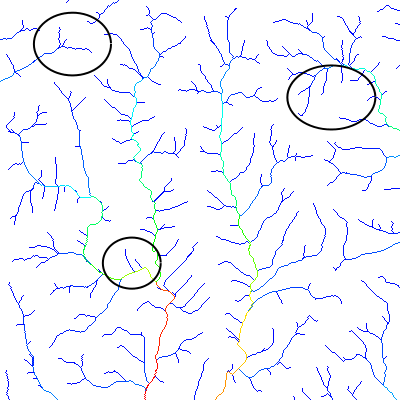
\includegraphics[width=\linewidth]{images/2DWithoutThresholdWeighting_mtn3_annotated.png}
\end{center}
\end{minipage}
&
\begin{minipage}[b]{0.45\linewidth}
\begin{center}
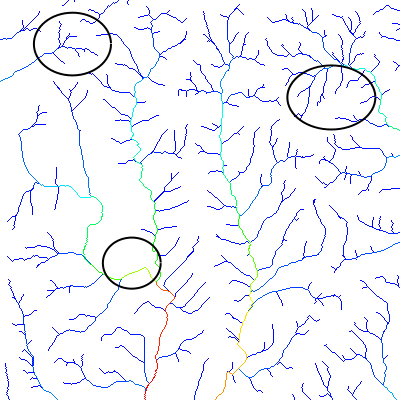
\includegraphics[width=\linewidth]{images/2DWithThresholdWeighting_mtn3_annotated.png}
\end{center}
\end{minipage} 
\end{tabular}
\caption[Two channel networks on MTN3, one without weighting and the other with.]{\label{figure:WithAndWithoutThresholdWeights} Two channel networks on the MTN3 dataset. The network to the left is extracted without using threshold weighting, while the network to the right does use it. Notice that as weighting is added, channels in higher elevations stretch for longer while channels along lower and flatter portions of the terrain disappear or become shorter. }
\end{figure*}


\begin{algorithm}[t]
\begin{algorithmic}
  \FOR{$\textbf{p} = 0 \to |T|$}
    \IF{$FlowAccum( \textbf{p} ) > 0$}
      \STATE $\textbf{p}' = lowestNeighbor( \textbf{p} )$
      \STATE $FlowAccum( \textbf{p}' ) \gets originalFlow( \textbf{p}' )$
    \ENDIF
  \ENDFOR 
\end{algorithmic}
\caption[Algorithm to fill in the gaps left by the flow threshold weighting scheme]{\label{algorithm:ChannelGapFilling}The algorithm to fill in the gaps left by the flow threshold weighting scheme.}
\end{algorithm}

Because the weighting scheme is applied to a single pixel at a time, ignoring neighbor information, it is possible that gaps appear in the channel network. Because we can assume that water flow is continuous (as discussed above), these gaps can be repaired easily. The method used is described in Algorithm \ref{algorithm:ChannelGapFilling}. Every pixel along a flow path between a source and its sink is considered part of the network.
% 
Algorithm \ref{algorithm:ChannelGapFilling} can either be applied to pixels in elevation order, or iteratively until no new pixels are discovered. 
% What we have left is a matrix of pixels belonging to the channel network. Once this matrix of channel network pixels is populated, further analysis of the network becomes possible.

Once the pixels of the channel network have been identified, the drill representation of the terrain can be determined.

\section{The Drill Representation}

For any given pixel on the terrain, $\textbf{p}_{i} \in T$, a drill shape is determined by fitting a curve to the channel profile at $\textbf{p}_{i}$, which then represents the shape of the widest drill that can conservatively fit in the channel.
The overall channel profile is represented by the union of all collected cross sections at $\textbf{p}_{i}$.
%  This process is depicted in Figure TBD. 

% \fbox{NEW IMAGE FOR NEW METHOD}

\subsection{Determining Drill Shape}

\begin{figure}[t]
\begin{center}
  \begin{minipage}{0.49\linewidth} 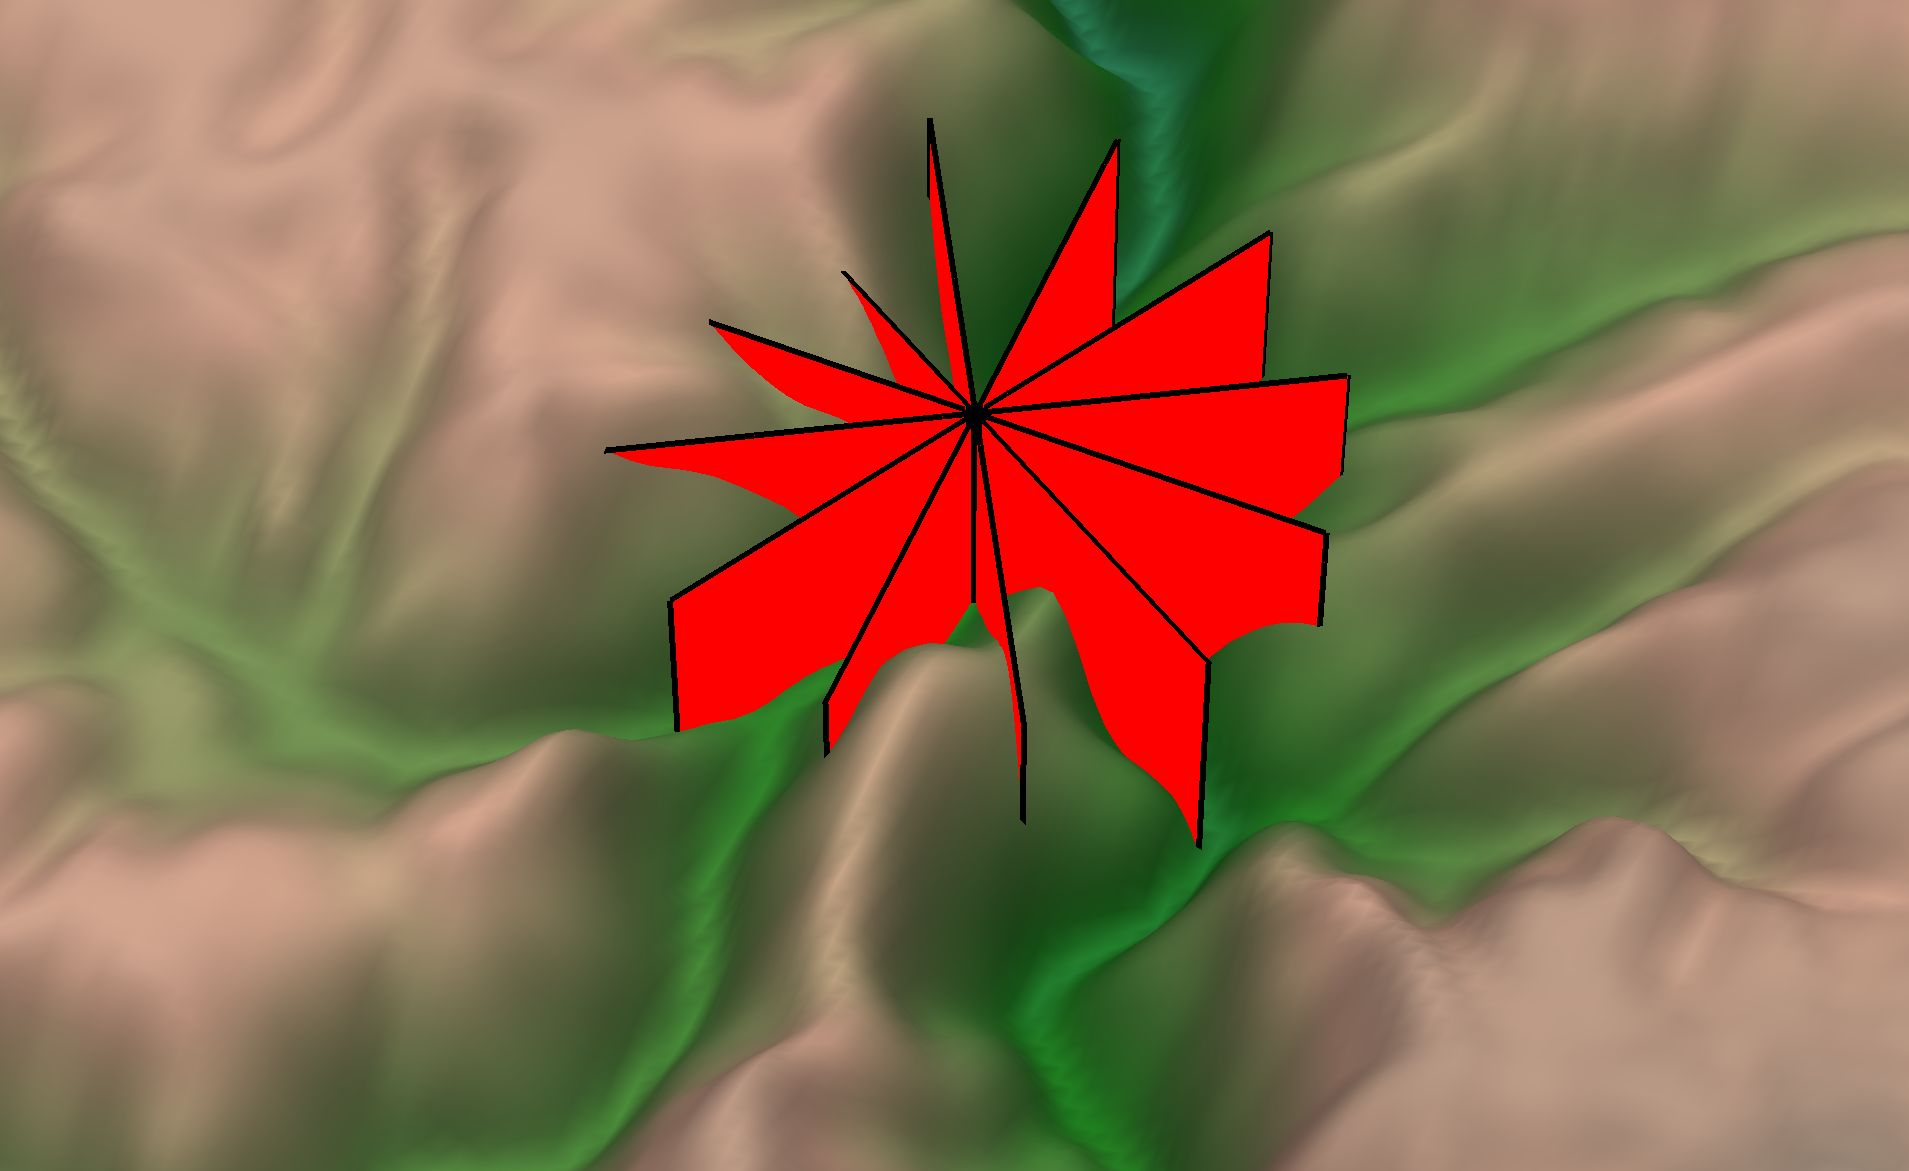
\includegraphics[width=0.99\linewidth]{images/crossSection.jpg}  \end{minipage}
  \begin{minipage}{0.49\linewidth} 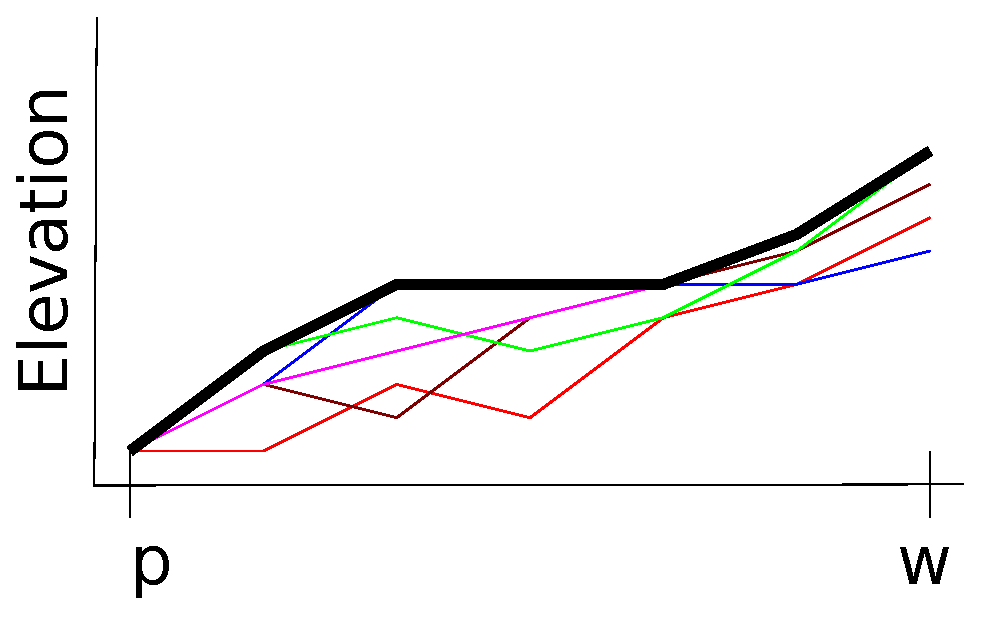
\includegraphics[width=0.99\linewidth]{images/CrossSections_2.eps} \end{minipage}
\end{center}
\caption[A visualization of the process of determining the union of the cross sections of the terrain's channels]{\label{figure:cross_section} A visualization of the process of determining the union of the cross sections of the terrain's channels. The left image depicts the process of gathering the cross sections. Each red plane is a cutting plane, and the cross section of the terrain determined by each one is collected. The right image depicts finding the union of all cross section. The colored thin lines represent the set of all cross sections at pixel $\bf{p}$, each one a collection of elevations of length $w$. The thick black line represents the final union.  }
\end{figure}

At each pixel $\textbf{p}_{i}$, a set of $c$ uniformly-spaced cross sections of the terrain are collected, where $c$ is an adjustable parameter. In this work, $c=120$ is an adequate value. This set of cross sections provides a profile of a channel at $c$ distinct angles. A sample of this procedure is shown in Figure \ref{figure:cross_section}. The cross sections span a distance $w$ from the center of $\textbf{p}_{i}$.
% , the second user-defined parameter to our system. 
The larger the value for $w$ is, the larger the area of influence on the terrain surface that is considered when determining the drill shape. For each pixel,
% in the channel network, 
uniformly spaced sample elevation points are collected in each direction along the crossing plane representing the cross section. Most of these sample points do not fall directly in the center of a pixel, and so simple bilinear interpolation is used to estimate the elevation of any sample point that does not exactly match a pixel center.

Once the set of cross sections is collected, its union is calculated by taking the maximum elevation value at each sampled distance from $\textbf{p}_{i}$, as depicted in Figure \ref{figure:cross_section}. This new terrain profile represents the widest that a drill can be in order to most accurately carve the terrain at $\textbf{p}_{i}$. 
The conservative estimate is necessary to guarantee that the terrain is not overly flattened by fitting a drill to a cross-section parallel to the channel length.
% , if the pixel is inside of a channel on the terrain.
Next, a curve is fit to the calculated union by treating the fitting as a constrained linear least-squares problem over the $w$ elevations of the union.
%  We constrain only the center point of the intersection, the elevation of $\textbf{p}_{i}$. The coefficients of this fitted quadratic equation represent the shape of the drill at $\textbf{p}_{i}$.
This fit curve can be of any family of functions the user desires. The coefficients of this function represent the encoding of the shape of the drill.
% , and are used to encode it.

% The terrain is completely represented by the list of pixels in the channel network and their associated drill's quadratic coefficients.


\subsection{Terrain Regeneration}

To regenerate the terrain from the drill representation, begin with a flat plateaued terrain of elevation $m$, where $m$ 
is the maximum elevation of $T$. A new terrain is procedurally generated by iteratively applying operations to this initial plateau, $T_{0}$. 
The $i^{th}$ 
drill
%, which corresponds with a pixel $\textbf{p}_{i}$ in the channel network of $D$, 
is represented by a $2k + 1 \times 2k + 1$ matrix 
$D_{i}$, where $k$ is referred to as the drill's ``influence''. Essentially, this is how large of an area of the terrain each drill operation 
affects.
% , and is the third and final user-defined parameter to the system. 
The width and height of $D_{i}$ must be odd because it must have a ``center'' pixel.

In order to drill the terrain, $D_{i}$ is centered over pixel $\textbf{p}_{i}$. The procedural generation is defined in Equation \ref{equation:drill}:

\begin{equation}
\label{equation:drill}
  T_{i} = \min\left( T_{i-1}, D_{i} \right)
\end{equation}

\noindent where the $\min\left(\right)$ function operates over the $2k + 1 \times 2k + 1$ area of $D_{i}$ and outputs a new matrix of minimum values between the pixels of $D_{i}$ and corresponding pixels of $T_{i-1}$. The resulting terrain has been drilled, and the process is repeated for the next operation, until all drills have been applied.
% The results of this procedural generation can be seen in Figure \ref{figure:lowest_errors}.




\section{Measuring Terrain Distances}
\label{section:TerrainDistances}

% It is necessary to have 
A quantitative measure of the difference between two terrain datasets, specifically height fields, $T_{0}$ and $T_{1}$, is necessary 
in order to judge the accuracy of terrain compression schemes and data representations (such as the drill operator presented in Chapter \ref{chapter:DrillOperator}).
Therefore, the notion of \textit{terrain distance}, or \textit{terrain dissimilarity}, must be explored. This chapter will present a series of metrics that determine $d\left(T_{0}, T_{1}\right)$, the distance between two height field datasets.

\subsection{Description of Distance Metrics}
\label{section:DescriptionOfMetrics}

Traditional distance metrics for spatial datasets, such as terrain surfaces, include Root Mean Square Error (RMSE) and Slope Surface RMSE (SSRMSE). These metrics provide a measure of 
% precision and accuracy lost 
distance on a global scope but ignore what can be thought of as the ``important'' characteristics of terrain, such as the shape and behavior of watersheds and channel networks,
and have been used to judge the accuracy of compression schemes and terrain representations (Stookey et al. \cite{Stookey08parallelodetlap}).


RMSE measures the root of the average squared difference in heights across the terrain, as shown in Equation \ref{equation:RMSMetric}:

\begin{equation}
\label{equation:RMSMetric}
%   RMSE\left(T_{0}, T_{1}\right) = \sqrt{ \frac{\displaystyle\sum_{\textbf{p}\in T_{0}, \textbf{q} \in T_{1}}{ \left(\textbf{p}_{z} - \textbf{q}_{z} \right)^2 } }{ |T_{0}| } }
  RMSE\left(T_{0}, T_{1}\right) = \sqrt{ \dfrac{\displaystyle\sum_{x < X} \displaystyle\sum_{y < Y} { \left( T_{0}\left(x,y\right) - T_{1}\left(x,y\right) \right)^2 } }{ X * Y } }
\end{equation}

\noindent where $X$ and $Y$ are the dimensions of $T_{0}$ and $T_{1}$, $T_{0}\left(x, y\right)$ is the elevation value at position $\left(x, y\right)$.
% , and 
% $z_{max}$ and $z_{min}$ are the maximum and minimum elevations of the pixels of $T_{0}$. 
% $|T_{0}|$ is the number of pixels in $T_{0}$.
This metric provides a single global distance measurement when comparing two datasets.
% , normalized by the value range of the pixels in $T_{0}$.

% % % For any two sets of pixels (in this case, the sets of all pixels in the channel network of each terrain), AHD finds  the maximum value of the average of the infimum of the
% % % distances between the sets,
% % % % the average of the shortest distance between their pixels, 
% % % as shown in Equation \ref{equation:hausdorffAvg}:
% % % 
% % % \begin{equation}
% % % \label{equation:hausdorffAvg}
% % % d_{ave} \left( N^{T_{0}}_{\tau}, N^{T_{1}}_{\tau} \right) = \max\left\{ \overline{\inf_{\textbf{p}_{j} \in N^{T_{1}}_{\tau}, \textbf{p}_{i} \in N^{T_{0}}_{\tau}} d\left(\textbf{p}_{i}, \textbf{p}_{j}\right)}, \overline{\inf_{\textbf{p}_{i} \in N^{T_{0}}_{\tau}, \textbf{p}_{j} \in N^{T_{1}}_{\tau}} d\left( \textbf{p}_{i}, \textbf{p}_{j} \right)} \right\}
% % % \end{equation}
% % % 
% % % \noindent where $N^{T_{0}}_{\tau}$ is the $i^{th}$ pixel of the set of channel network pixels extracted using threshold $\tau$, and $d\left( \textbf{p}_{i}, \textbf{p}_{j} \right) $ is
% % % the Euclidean distance between pixels $\textbf{p}_{i}$ and
% % % $\textbf{p}_{j}$. 
% % %  This metric tends to give a much more
% % % realistic look at the channel networks' distances.
% 
% 

% The slope surface RMSE metric measures the RMSE in the slope values at each pixel. To measure the SSRMSE, a slope surface is created by measuring the slope at each pixel. For each pixel $\textbf{p}_{i} = \left(x_{i}, y_{i}\right)$, the slope values is determined by Equation \ref{equation:PixelSlopeValue}:
% 
% \begin{equation}
% \label{equation:PixelSlopeValue}
%   \Delta_{xy} \left( \textbf{p}_{i} \right) = \dfrac{ |\left( \left( x_{i} + 1, y_{i}\right)_{z} - \left(x_{i} - 1, y_{i} \right)_{z} \right)| + |\left( \left( x_{i}, y_{i} + 1\right)_{z} - \left(x_{i}, y_{i} - 1 \right)_{z} \right)| }{2}
% \end{equation}
% 
% SSRMSE measures the RMSE between the slope surfaces of $T_{0}$ and $T_{1}$, $S_{T_{0}}$ and $S_{T_{1}}$, respectively. This is described in Equation \ref{equation:SSRMSE}
% 
% \begin{equation}
% \label{equation:SSRMSE}
%   SSRMSE\left(T_{0}, T_{1}\right) = RMSE\left(S_{T_{0}}, S_{T_{1}}\right)
% \end{equation}


RMSE provides a measure of elevation error, but oftentimes the more important characteristic of the terrain is the overall shape of the surface. Its shape determines the terrain's hydrography information, as well. The following metrics provide quantitative measurements of the dissimilarity between terrain shapes.

The gradient of the surface at each pixel is the determining factor in the flow of water across the terrain. Therefore, it is useful to measure the distance between the shapes of two terrain surfaces. In this work, the slope defined by Zevenberger-Thorne \cite{ESP:ESP3290120107} and the method presented by Tracy \cite{Tracy:2009:PPS:1751402} is used as a measure of slope dissimilarity. This measure requires finding the vector normal to the surface at each pixel (the vector perpendicular to the gradient direction, or tangent, of the surface). The normal at each corresponding pixel is found, and the angle between the vectors is measured. The average of these angles across the entire terrain provides a value for the distance, $SSE\left(T_{0}, T_{1}\right)$.

% 
% \begin{equation}
%   SSE\left(T_{0},T_{1}\right) = 
% \end{equation}



Both SSE and RMSE provide a measure of global distances between two spatial datasets. However, when measuring the distance between two terrain datasets, it is often more appropriate to determine how dissimilar specific characteristics of the terrain are from one another.

The following metrics take as input two channel networks
($N^{T_{0}}_{\tau}$ and $N^{T_{1}}_{\tau}$) and return the distance between
them. These metrics are used to help define the difference between the
terrains and thresholds from which the networks result. 
% % Since the metrics have been designed to 
% % take in any channel networks, comparisons between terrains
% % from simulation data (different time steps in the same sequence), between unrelated terrains, or even
% the same terrain with networks formed using different thresholds are possible.

% \subsection{Pixel-to-Pixel Correspondence Metric}
% \label{section:PixelToPixelCorrespondence}

The first metric is the pixel to pixel correspondence metric, described in equation \ref{equation:pix_dist}, in which
each pixel of $N^{T_{0}}_{\tau}$ is compared to each in $N^{T_{1}}_{\tau}$,
and two pixels are said to correspond if 
% their addresses have the same length (meaning 
they are each the same depth in their respective networks,
and their flow travels in the same direction. 
% I do not compare
% addresses directly because of potential inconsistencies in the
% labeling scheme applied to two similar but not identical networks.
% A slight change in threshold can cause a new, very small network to
% form elsewhere in the terrain, and as a result the ID system for the
% networks (Figure \ref{figure:addressingScheme}) is not comparable
% between thresholds, only a pixel's position within its own network.

\begin{align}
\label{equation:pix_dist}
  d_{pix} \left( N^{T_{0}}_{\tau}, N^{T_{1}}_{\tau} \right) = \dfrac{ \left| \left\{ \textbf{p}_{i} \  | \ \textbf{p}_{i} \rightarrow \textbf{p}_{j} \right\} \right| }{ \left| N^{T_{0}}_{\tau} \right|  }
\end{align}

\noindent where $\textbf{p}_{i} \in N^{T_{0}}_{\tau}\,$ and
$\textbf{p}_{j} \in N^{T_{1}}_{\tau}$ is its corresponding pixel (same x,
y coordinates in its respective terrain), and $\left| N^{T_{0}}_{\tau}
\right|$ is the total number of pixels compared, a normalizing
component.

% One major shortcoming of the pixel-to-pixel correspondence metric is that a small change in the network downstream of any pixel has the potential to drastically change the address assigned to the pixel. For this reason, the use of this metric should be limited to major channel networks after a pruning procedure has taken place. Thus, 
Pixels of similar networks correspond regarding their positions in the network, and thus this metric is a normalized count of the number of correlated pixels between two networks. This metric also inherently uses channel length as a measure of dissimilarity.

% \subsection{Hausdorff Distance Metrics}citeulike:1146653
% \label{section:HausdorffDistanceMetrics}

The second metric is an adaptation of the traditional \emph{Hausdorff distance} metric, defined in equation \ref{equation:hausdorff}.

\begin{align}
\begin{split}
\label{equation:hausdorff}
& d_{haus} \left( N^{T_{0}}_{\tau}, N^{T_{1}}_{\tau} \right) =  
\max \left\{ \sup_{ \textbf{p}_{i} \in N^{T_{0}}_{\tau} } \inf_{ \textbf{p}_{j} \in N^{T_{1}}_{\tau} } d\left( \textbf{p}_{i} \, \textbf{p}_{j} \right) \, \sup_{ \textbf{p}_{j} \in N^{T_{1}}_{\tau} } \inf_{ \textbf{p}_{i} \in N^{T_{0}}_{\tau} } d\left( \textbf{p}_{i} \, \textbf{p}_{j} \right) \right\}
%  \max\left\{ \overline{\inf_{\textbf{p}_{j} \in N^{T_{1}}_{\tau}, \textbf{p}_{i} \in N^{T_{0}}_{\tau}} d\left(\textbf{p}_{i}, \textbf{p}_{j}\right)}, \overline{\inf_{\textbf{p}_{i} \in N^{T_{0}}_{\tau}, \textbf{p}_{j} \in N^{T_{1}}_{\tau}} d\left( \textbf{p}_{i}, \textbf{p}_{j} \right)} \right\}
\end{split}
\end{align}

\noindent where $d\left( \textbf{p}_{i}, \textbf{p}_{j} \right) $ is
the Euclidean distance between pixels $\textbf{p}_{i}$ and
$\textbf{p}_{j}$. The Hausdorff distance metric is a measure over all of the pixels in each channel network. It is defined as the maximum distance of the set of minimum distances between a pixel $\textbf{p}_{i}$ in $N^{T_{0}}_{\tau}$ and the pixels in $N^{T_{1}}_{\tau}$. However, due to the nature of the metric, it can lend too much weight to outliers. Therefore, a third metric, the average Hausdorff distance as proposed by Dubuisson and Jain \cite{citeulike:1146653}, is used.

For any two sets of pixels, the average Hausdorff metric finds the average of the shortest distance between their respective pixels, as shown in Equation \ref{equation:hausdorffAvg}:
%  the average Hausdorff distance metric, as described by Equation \ref{equation:hausdorffAvg}.

\begin{align}
\label{equation:hausdorffAvg}
\begin{split}
& d_{avg} \left( N^{T_{0}}_{\tau}, N^{T_{1}}_{\tau} \right) = 
% \max \left\{ \overline{ \inf_{\textbf{p}_{j} \in N^{T_{1}}_{\tau} \textbf{p}_{i} \in N^{T_{0}}_{\tau} } d\left( \textbf{p}_{i}, \textbf{p}_{j} \right) }, \overline{ \inf_{\textbf{p}_{i} \in N^{T_{0}}_{\tau}, \textbf{p}_{j} \in N^{T_{1}}_{\tau} } d\left( \textbf{p}_{i}, \textbf{p}_{j} \right) } \right\}
 \max\left\{ \overline{\inf_{\textbf{p}_{j} \in N^{T_{1}}_{\tau}, \textbf{p}_{i} \in N^{T_{0}}_{\tau}} d\left(\textbf{p}_{i}, \textbf{p}_{j}\right)}, \overline{\inf_{\textbf{p}_{i} \in N^{T_{0}}_{\tau}, \textbf{p}_{j} \in N^{T_{1}}_{\tau}} d\left( \textbf{p}_{i}, \textbf{p}_{j} \right)} \right\}
\end{split}
\end{align}

\noindent where 
$\textbf{p}_{i} \in N^{T_{0}}_{\tau}$ is the $i^{th}$ pixel of the set of channel network pixels 
of $T_{0}$ extracted using threshold $\tau$, $N^{T_{0}}_{\tau}$. The overline means ``mean value of''. 
It is important to note that AHD is limited to the channel networks of the terrain, whereas RMSE is applied globally. 
Limiting RMSE to only $N_{\tau}$ would not give an accurate picture of how close the terrains' hydrography networks are, 
since the network pixels are found by looking at the global flow pattern. Even if the elevations of the pixels in $N_{\tau}$ 
are comparable, it does not indicate that the overall terrain shape is similar. In addition, slight variations 
in the location of the pixels in $N_{\tau}$ would render RMSE unusable.

% \noindent or the maximum value of the average of the infimum of the
% distances between the sets. This metric tends to give a much more
% realistic look at the channel networks' distances, as it smooths out inaccurate distances created by outliers. 


The average Hausdorff distance provides a general picture of how close the pixels in $N^{T_{0}}_{\tau}$ are to those in $N^{T_{1}}_{\tau}$. It is important to note that this is a Euclidean metric, based on their exact positions in $\mathbb{R}^{3}$. All information regarding the geometry of the channel network (such as slope), meander, or flow is ignored. However, unlike the RMS Error metric, the average Hausdorff distance is a measurement of the geometric distance between only the pixels in the channel network, and thus it places emphasis on them and ignores the rest of the terrain. In this way, ``unimportant'' elevation information and outliers are not taken into account. By limiting the metric to pixels in the channel network, the geometry of the entire terrain is inherently incorporated but weighted by distance and contribution to the channel network.
% , because it is all data critical to the formation of the channel network, while focusing the metric on the important pixels.

Another hydrography-specific metric employed in this thesis is the Ridge-River metric, proposed by Muckell et al. \cite{Muckell:2009:EHP:1517463.1517470}, $d_{RR}$. This metric measures the error in the overall structure of the flow network of a regenerated terrain by measuring the energy required by water to flow across the original terrain $T_{0}$ given the flow directions for the pixels in $T{1}$. In essence, the metric measures how poorly the flow network of $T_{1}$ fits $T_{0}$ when overlayed on top of it. Two separate energies are calculated: the total flow uphill, and the total flow downhill. These can be written as:

\begin{align}
  \label{equation:EnergyDown}
  EnergyDown & = \displaystyle\sum_{x < X} \displaystyle\sum_{y < Y} \text{max} \left( 0, T_{0}\left(x,y\right) - T_{0}\left(r\left(x,y\right)\right) \right) * flowAccum_{\left(x,y\right)} \\
  EnergyUp & = \displaystyle\sum_{x < X} \displaystyle\sum_{y < Y} \text{max} \left( 0, T_{0}\left(r\left(x,y\right)\right) - T_{0}\left(x,y\right) \right) * flowAccum_{\left(x,y\right)} \\
%   d_{RR} & = 
% 
%   EnergyDown & = \displaystyle\sum_{\textbf{p}\in T_{0}, \textbf{q} \in T_{1}} \text{max}\left( 0, E_{i} - E_{r\left(i\right)} \right) * flowAccum_{i} \\
%   EnergyUp & = \displaystyle\sum_{\textbf{p}\in T_{0}, \textbf{q} \in T_{1}} \text{max}\left( 0, E_{r\left(i\right)} - E_{i}  \right) * flowAccum_{i} \\
  d_{RR} \left( N^{T_{0}}_{\tau}, N^{T_{1}}_{\tau} \right) & = \dfrac{EnergyUp}{EnergyDown}
\end{align}

\noindent where $r\left(x,y\right)$ is the pixel that receives flow from pixel $\left(x,y\right)$ on $T_{1}$. The energies are calculated by summing the measured elevation increase for water flowing uphill (or downhill for $EnergyDown$), weighted by the total flow accumulation of pixel $\left(x,y\right)$ on $T_{1}$. 

Because the method for extracting $T_{0}$'s hydrography results in some uphill flow, $d_{RR}$ is calculated for the original terrain's hydrography network as well. This value is subtracted from $T_{1}$'s $d_{RR}$ for the final error measurement, thus providing a measure of how much hydrography error is introduced by the regeneration.


\subsection{Finding an Optimal Flow Threshold}

Once a definition of the distance between two terrains has been determined, then an optimal threshold value that minimizes the distance between two terrains can be found. 
% 
% A good deal of work has been done with the intent of finding an \emph{optimal} flow accumulation value with which to threshold the flow accumulation matrix to extract the channel network. 
There have been attempts to use drainage density (a ratio of flow value to pixel watershed size) as a value to threshold instead of flow accumulation, while others have attempted to use local curvature or gradient values, as discussed in section \ref{section:ChoosingAFlowThreshold}. 


A simple brute force method will find this threshold among a set of terrains, by trying several different thresholds for the terrains in question and recording those that produce the smallest distances.
What is a more interesting challenge is finding the optimal threshold to apply to each terrain in a sequential series. 
If there are several terrains that belong to a series (such as time steps in an erosion simulation, or several regenerated terrains that had been compressed with various parameters), $\{ T_{i} \}$, finding an optimal threshold to compare their channel networks requires a degree of sequential coherence so that networks change smoothly as one moves from one terrain to another.
% 
% 
% It is clear that this is an interesting and important avenue of research. With this in mind, I introduce 
% Therefore, a method for finding the optimal flow threshold with which to compare two terrains, $T_{i}$ and $T_{j}$ in a sequence is introduced.
% representing sequential time steps, $D_{i}$ and $D_{j}$, in a series of datasets from our erosion simulation. This procedure is limited to this situation because of the limited nature of the metrics presented in section \ref{section:DescriptionOfMetrics}. Because they apply best when two terrains should match closely with only minute differences, comparing two sequential datasets is an ideal situation.
% This algorithm works best when the extracted channel networks are similar to one another, such as when testing the accuracy of a compression scheme.

Despite the fact that $T_{i}$ and $T_{j}$ are assumed to be similar, the extracted channel networks are very sensitive to small changes in the chosen threshold value. Given this, the same threshold cannot necessarily be applied to $T_{i}$ and $T_{j}$, as there is no guarantee that the result channel networks will resemble one another.
%  (ADD IMAGE)
Additionally, when measuring the dissimilarity between a decompressed terrain and its baseline, small elevation errors may result in the same threshold resulting in significantly different channel networks. Therefore, a method for choosing threshold values for each terrain is important. 
% For the time being, I restrict its use to a series of temporally adjacent terrains in a series of time steps.

A moving window algorithm that can use any of the metrics introduced in section \ref{section:DescriptionOfMetrics} to determine the threshold that minimizes the distance between $T_{i}$ and $T_{j}$ is shown in algorithm \ref{algorithm:idealThreshold}.

\begin{algorithm}[t]
\begin{algorithmic}
  \STATE $avg \gets 0$
  \STATE $nComparisons \gets 0$
    \FOR{$w_{cur} = t - \mbox{\em WINDOW} \to t + \mbox{\em WINDOW}$}
      \FOR{$\tau = \tau_{min} \to \tau_{max}$}
	  \STATE $dist \gets d\left( N^{t}_{\tau}, N^{w_{cur}}_{\tau} \right)$
	  \STATE $avg \gets avg + \tau * c\left( dist \right)$
	  \STATE $nComparisons \gets nComparisons + 1$
     \ENDFOR
  \ENDFOR
  \STATE $avg \gets avg / nComparisons$
  \STATE return $avg$
\end{algorithmic}
\caption[The moving window algorithm for finding the ideal threshold.]{\label{algorithm:idealThreshold} The moving window algorithm for finding the ideal threshold between two terrains by comparing its channel network with those of its neighbors. {\em WINDOW} is a constant window size, $d\left(N^{t}_{\tau}, N^{w_{cur}}_{\tau} \right)$ is the distance between channel networks $N^{t}_{\tau}$ and $N^{w_{cur}}_{\tau}$, $[ \tau_{min}$, $\tau_{max} ]$ is the range of threshold values we wish to test, and $c\left( dist \right)$ is a weight applied to the distance between networks. A window size of 2 worked well for a 10-terrain sequence, and for $c$, a weight of 1 is often sufficient.}
\end{algorithm}

This method is limited by the nature of the windowing algorithm. Possible thresholds are tested across neighbors, but the sequential coherence may be adversely affected by the neighbors' choice for its threshold. 
% This windowing algorithm was used to determine the optimal thresholds to use 








% \chapter{Using the Drill Operator}
% \label{chapter:UsingTheDrillOperator}
% 
% The drill operator presented in chapter \ref{chapter:DrillOperator} provides a unique and novel method for representing the shape of a terrain surface. This chapter explores the operator's utility 
% by presenting various enhancements, applications, and uses for the drill operator with regard to accurately and compactly representing terrain data.
% % by presenting accuracy tests that show how closely the operator representation can mimic terrain data. These initial accuracy tests are followed by an in depth exploration of various expanded uses and applications of the drill operator.


\section{Initial Accuracy Trials}
\label{section:DrillAccuracyTests}

To determine the feasibility of representing terrain as drills, initial accuracy tests were performed to determine how closely the drill representation modeled the $400 \times 400$ mountainous dataset seen in Figure \ref{figure:mtn2_original}. All tests were performed in Ubuntu 11.04 with a quad-core AMD Phenom II X4 945 Processor, with 8GB of RAM. The code was written in MATLAB.

\subsection{Experimental Methodology}

The three parameters of the system, as described in Chapter \ref{chapter:DrillOperator}, are the threshold used to extract the original terrain's channel network $\tau$, the size of the cross section $w$, and the influence of a drill (size of the representative matrix) $k$. Each of 3 thresholds, 3 cross-section sizes, and 6 influence values were used to build regenerated terrains in the factorial experiment described in this section. 

For each set of parameter values, the total error between the generated terrain and the initial terrain was calculated using a measure for dissimilarity between the two sets.
These metrics take as input two channel networks
($N^{i}_{\tau}$ and $N^{j}_{\tau}$) and return the distance between
them.
 The two metrics used were the standard root mean squares error (RMSE) metric, and the averaged Hausdorff distance (AHD) metric as described in Section \ref{section:DescriptionOfMetrics}.
% by Stuetzle et al. \cite{stuetzle-TerrainDistances}, inspired by the shape analysis techniques discussed in Section \ref{section:ShapeAnalysisTechniques}.

It is important to note that AHD is limited to the channel networks of the terrain, whereas RMSE is applied globally. Limiting RMSE to only $N_{\tau}$ would not give an accurate picture of how close the terrains' hydrography networks are, since the network pixels are found by looking at the global flow pattern. Even if the elevations of the pixels in $N_{\tau}$ are comparable, it does not indicate that the overall terrain shape is similar. In addition, slight variations in the location of the pixels in $N_{\tau}$ would render RMSE unusable. Therefore, the results for both metrics are analyzed in context of their maximum error and what they mean from a physical standpoint.

\subsection{Results and Discussion of Initial Accuracy Trials}
\label{section:DrillAccuracyResultsAndDiscussion}

\begin{figure}
\begin{center}
  \begin{minipage}{0.49\linewidth}
     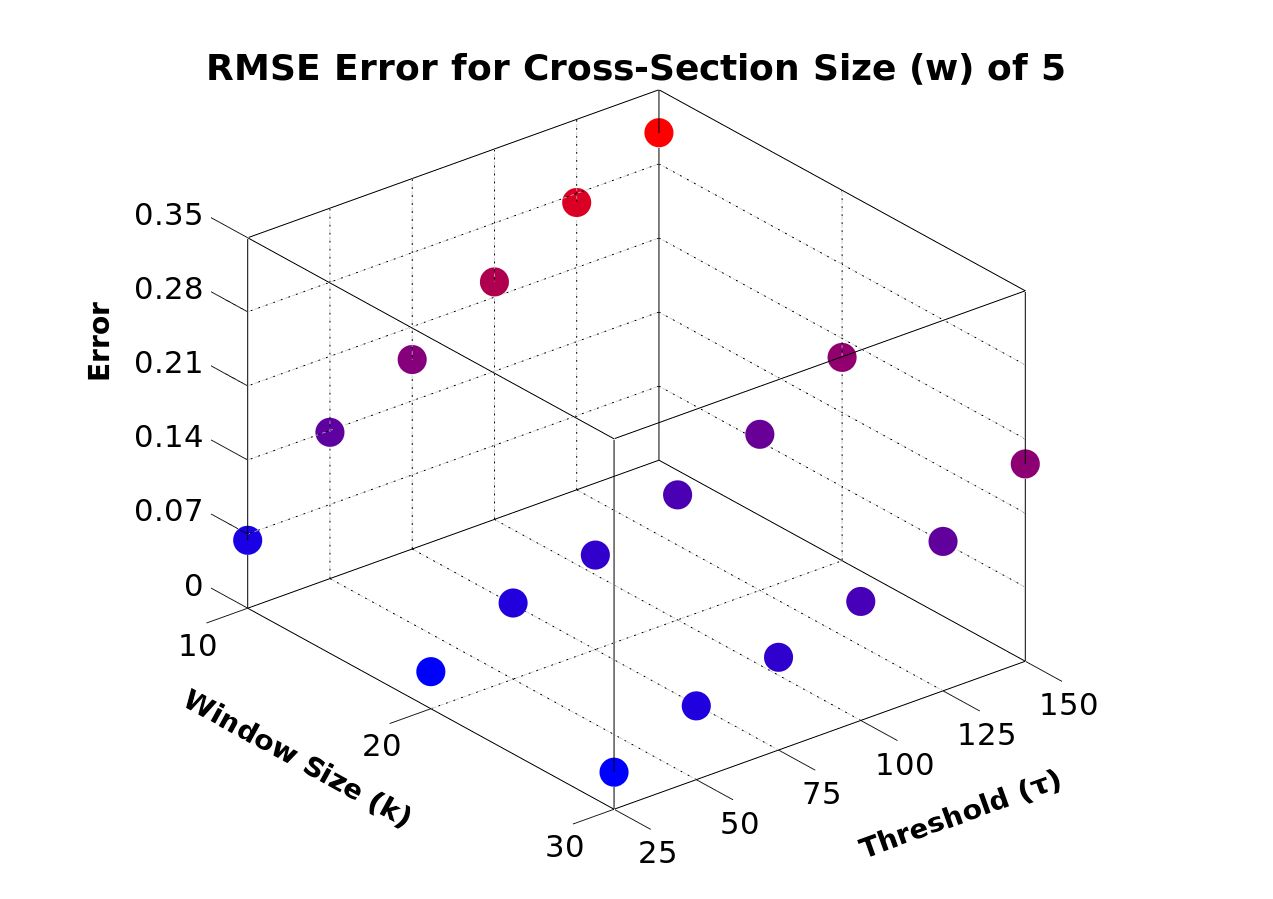
\includegraphics[height=0.25\textheight,width=0.99\linewidth]{images/RMSE_Graph_CS5.jpg} 

     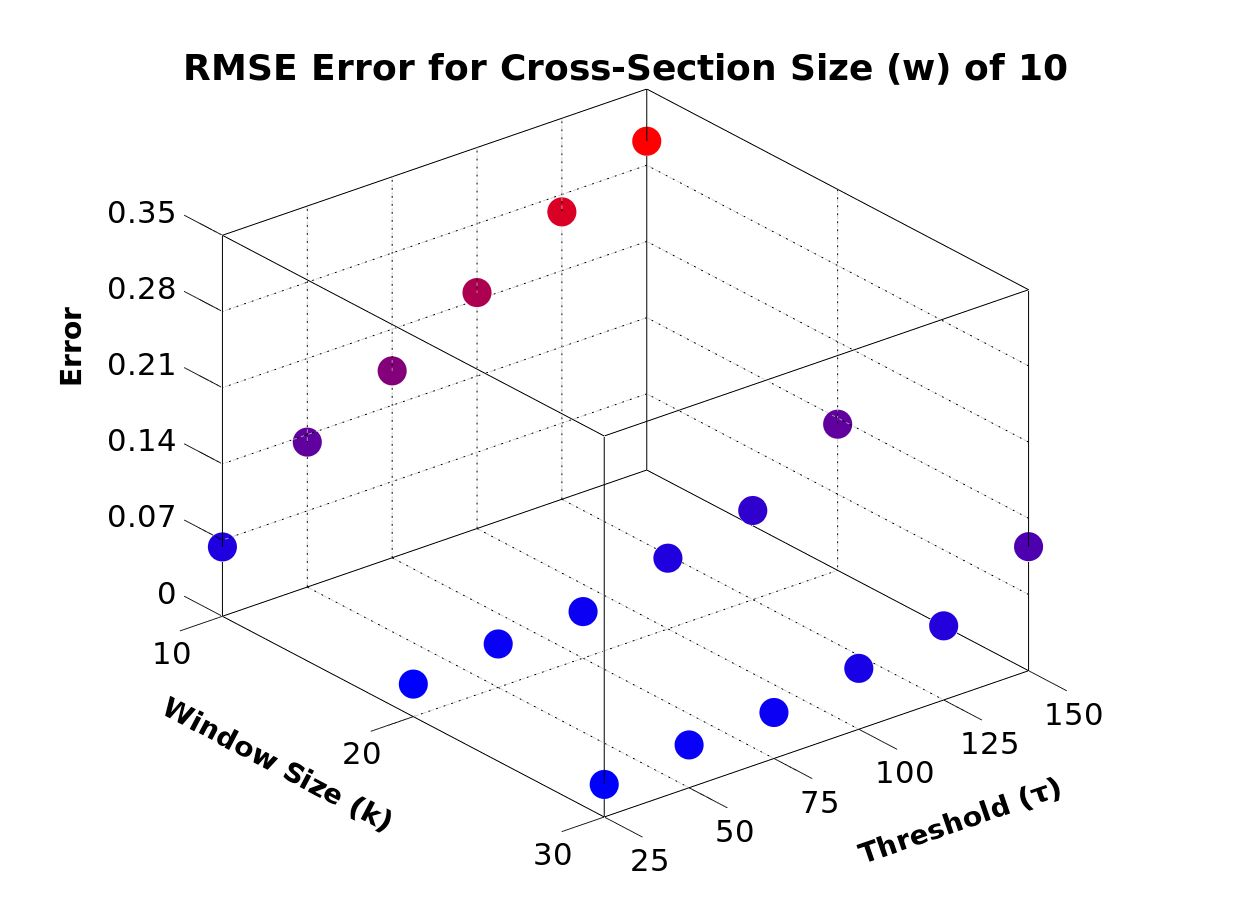
\includegraphics[height=0.25\textheight,width=0.99\linewidth]{images/RMSE_Graph_CS10.jpg}

     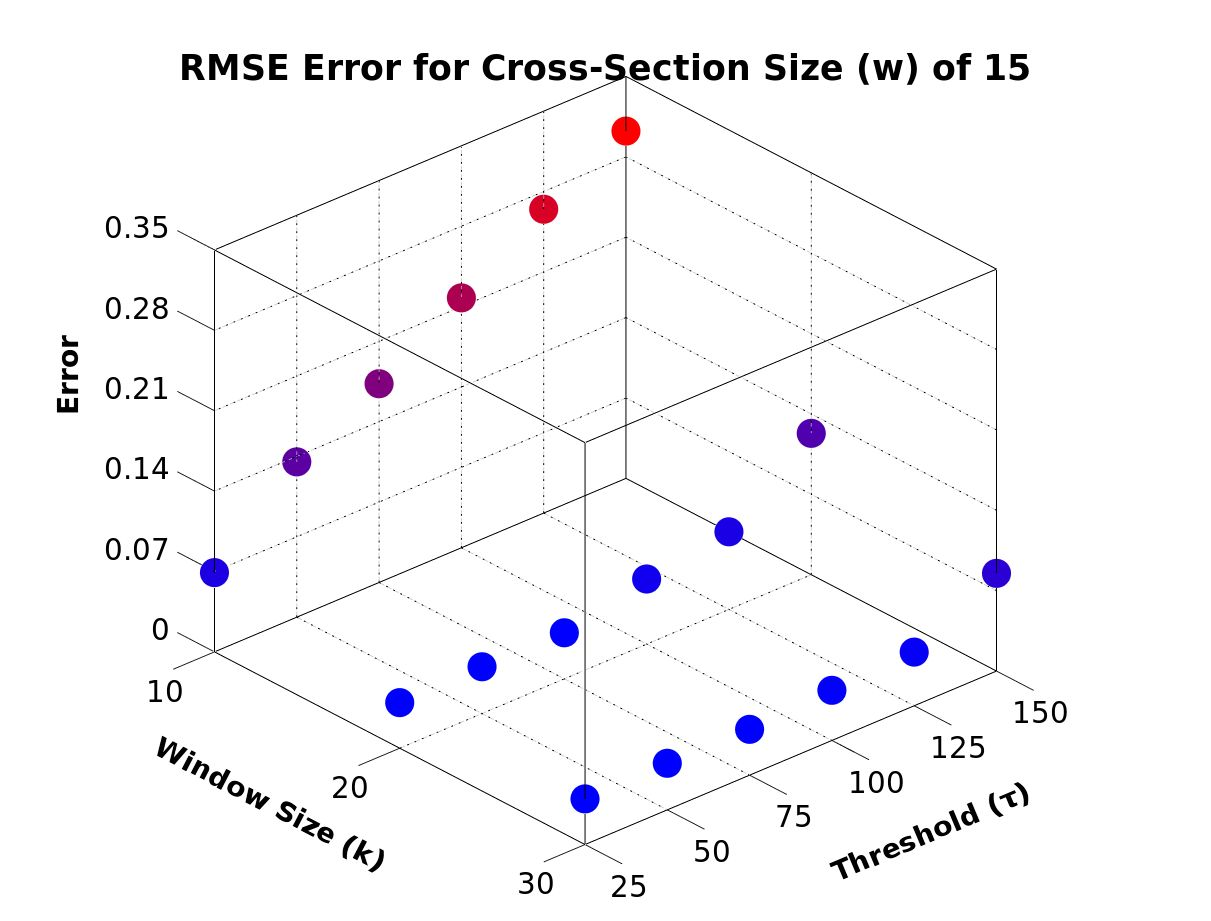
\includegraphics[height=0.25\textheight,width=0.99\linewidth]{images/RMSE_Graph_CS15.jpg}  
  \end{minipage}
  \begin{minipage} {0.49\linewidth} 
    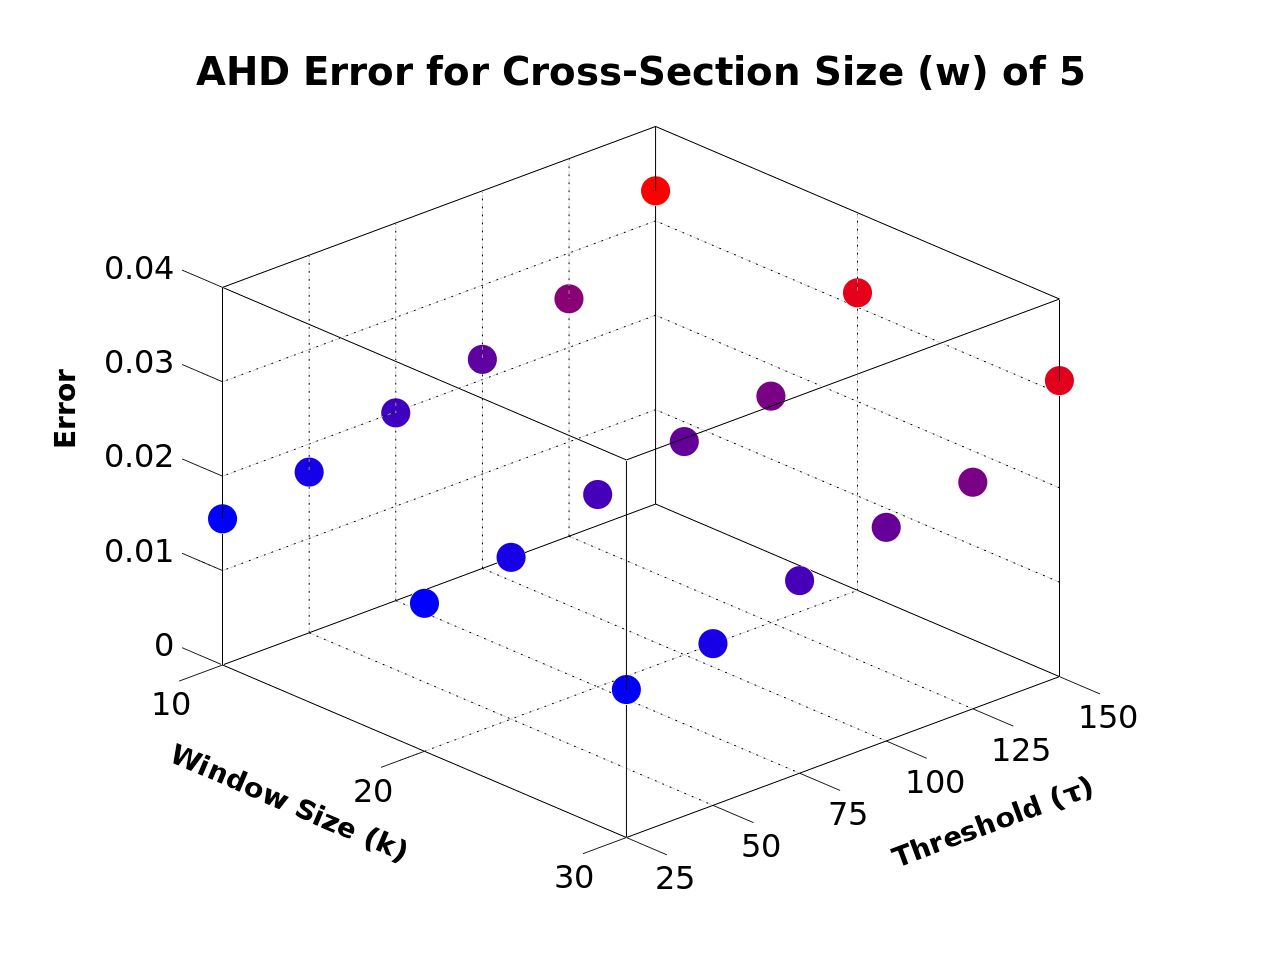
\includegraphics[height=0.25\textheight,width=0.99\linewidth]{images/AHD_Graph_CS5.jpg} 
 
    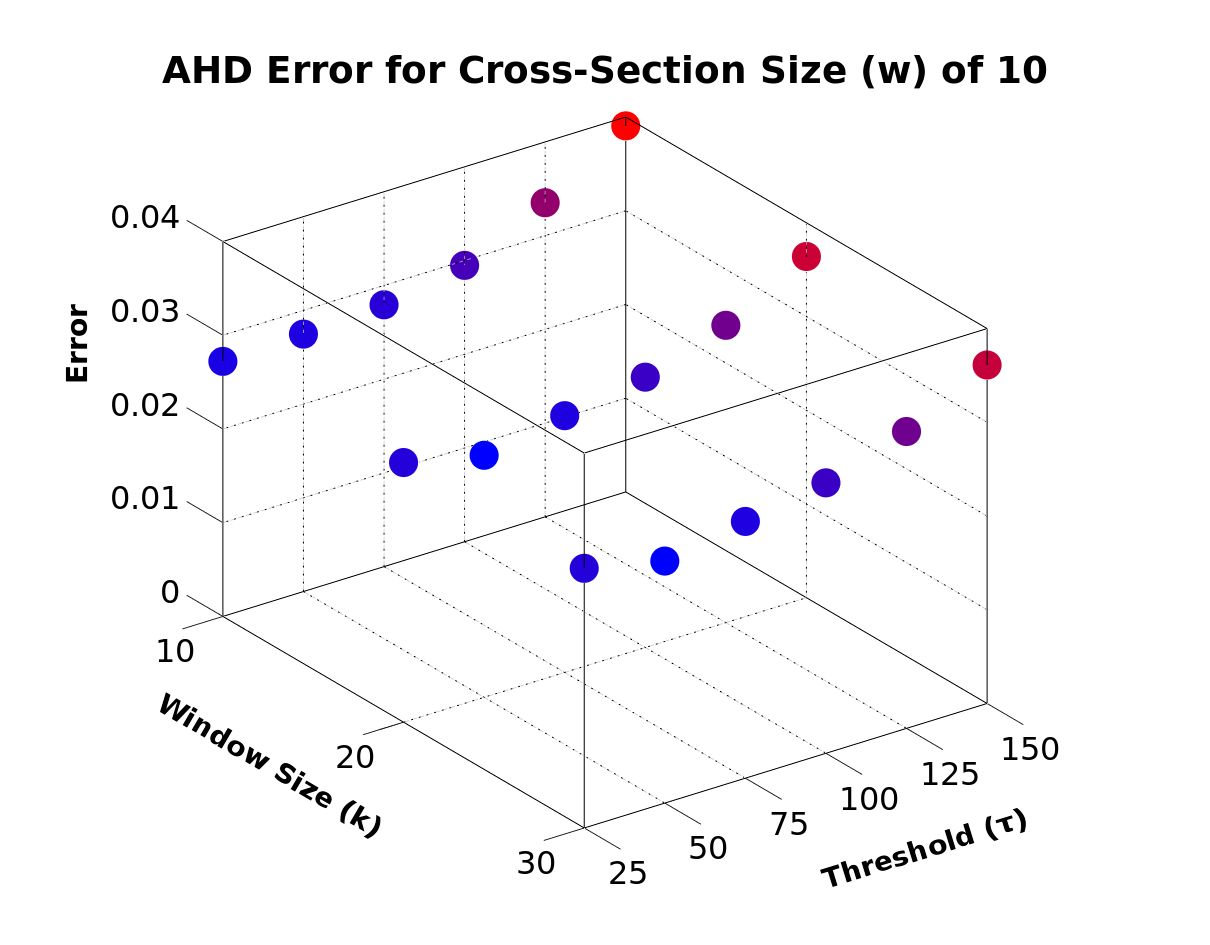
\includegraphics[height=0.25\textheight,width=0.99\linewidth]{images/AHD_Graph_CS10.jpg}

    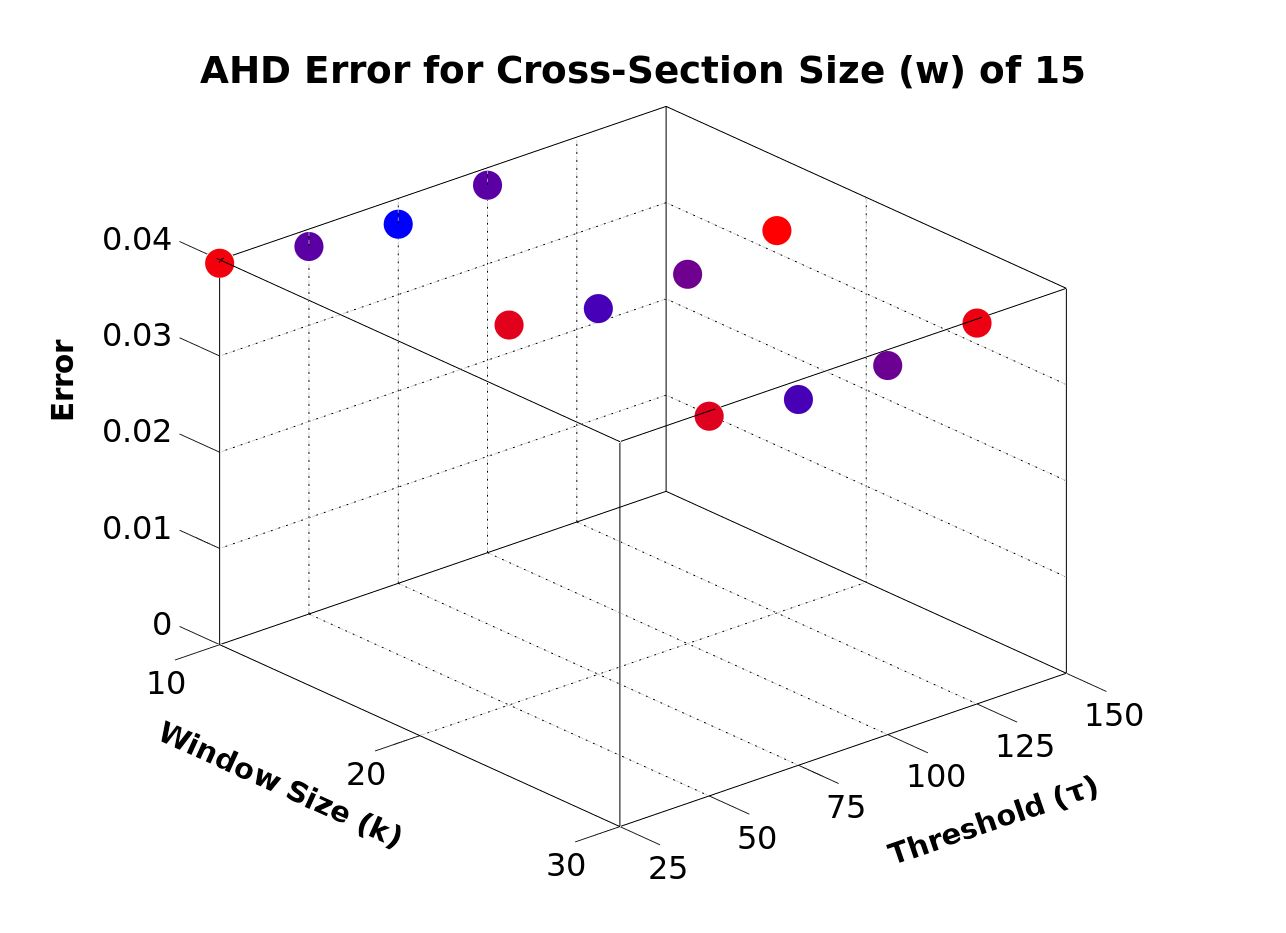
\includegraphics[height=0.25\textheight,width=0.99\linewidth]{images/AHD_Graph_CS15.jpg}
  \end{minipage}
\end{center}
\caption[The results for the concept tests for the drill operator]{\label{figure:results} The results of accuracy testing. The left column depicts the error measured using the RMSE metric, and the right column depicts error measured used the AHD metric. Each row shows a different value for the cross section window size (parameter $w$). Each metric's data is normalized. Red indicates high error, whereas blue indicates low error, local to each dataset.
\fbox{FIX LATER}}
\end{figure}


\begin{figure}[t]
\begin{center}
  \begin{minipage}{0.49\linewidth} 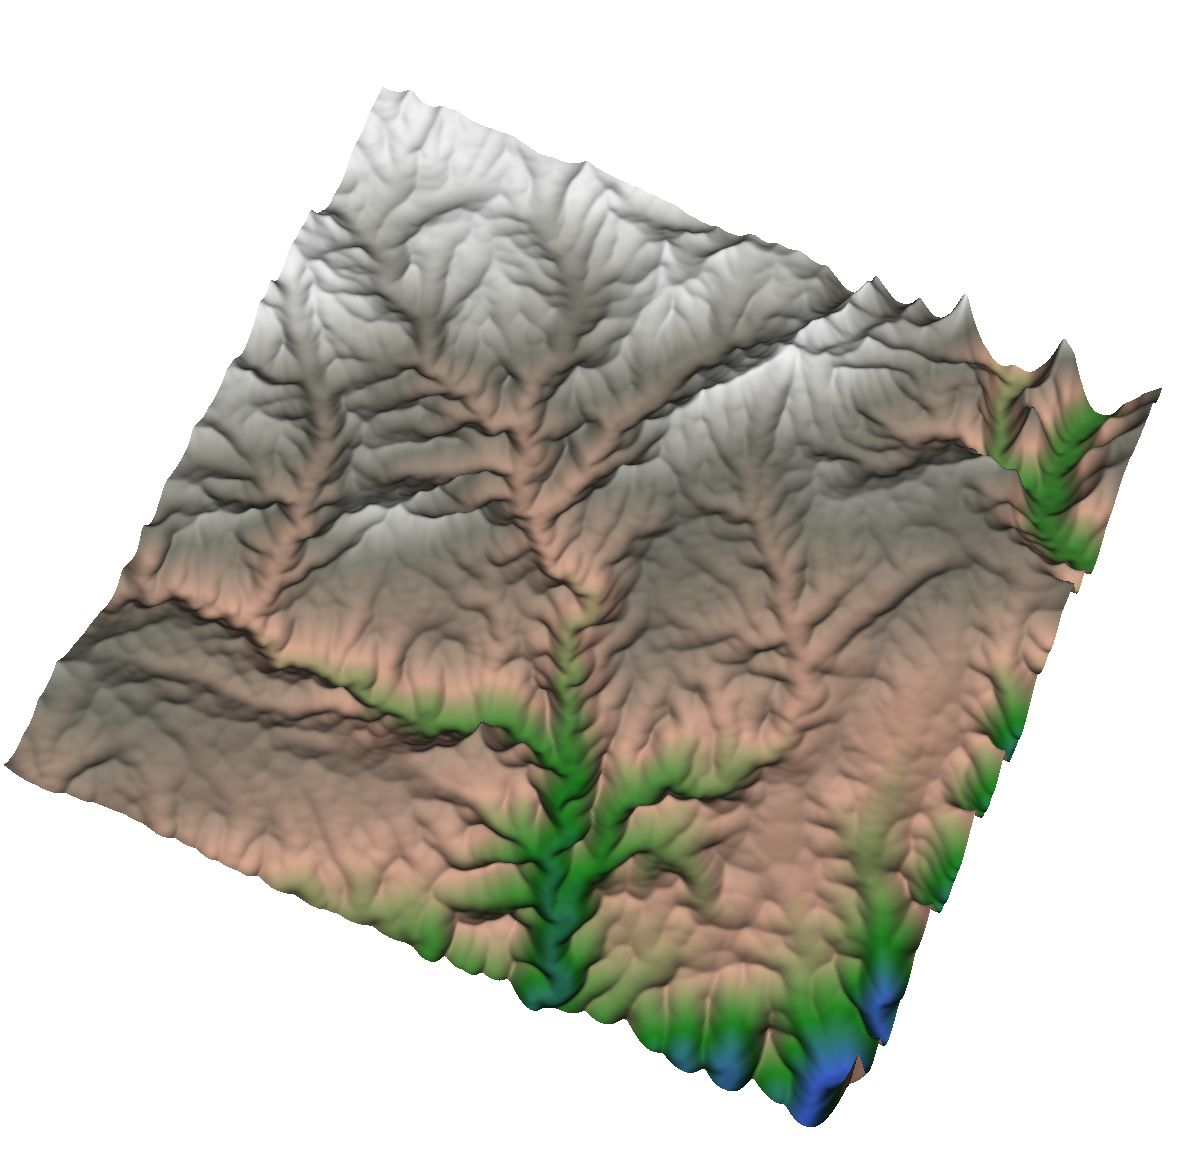
\includegraphics[width=0.99\linewidth]{images/W10_I20_T25.jpg} \\ \centering $\tau=25$, $w=10$, $k=20$ \end{minipage}
  \begin{minipage}{0.49\linewidth} 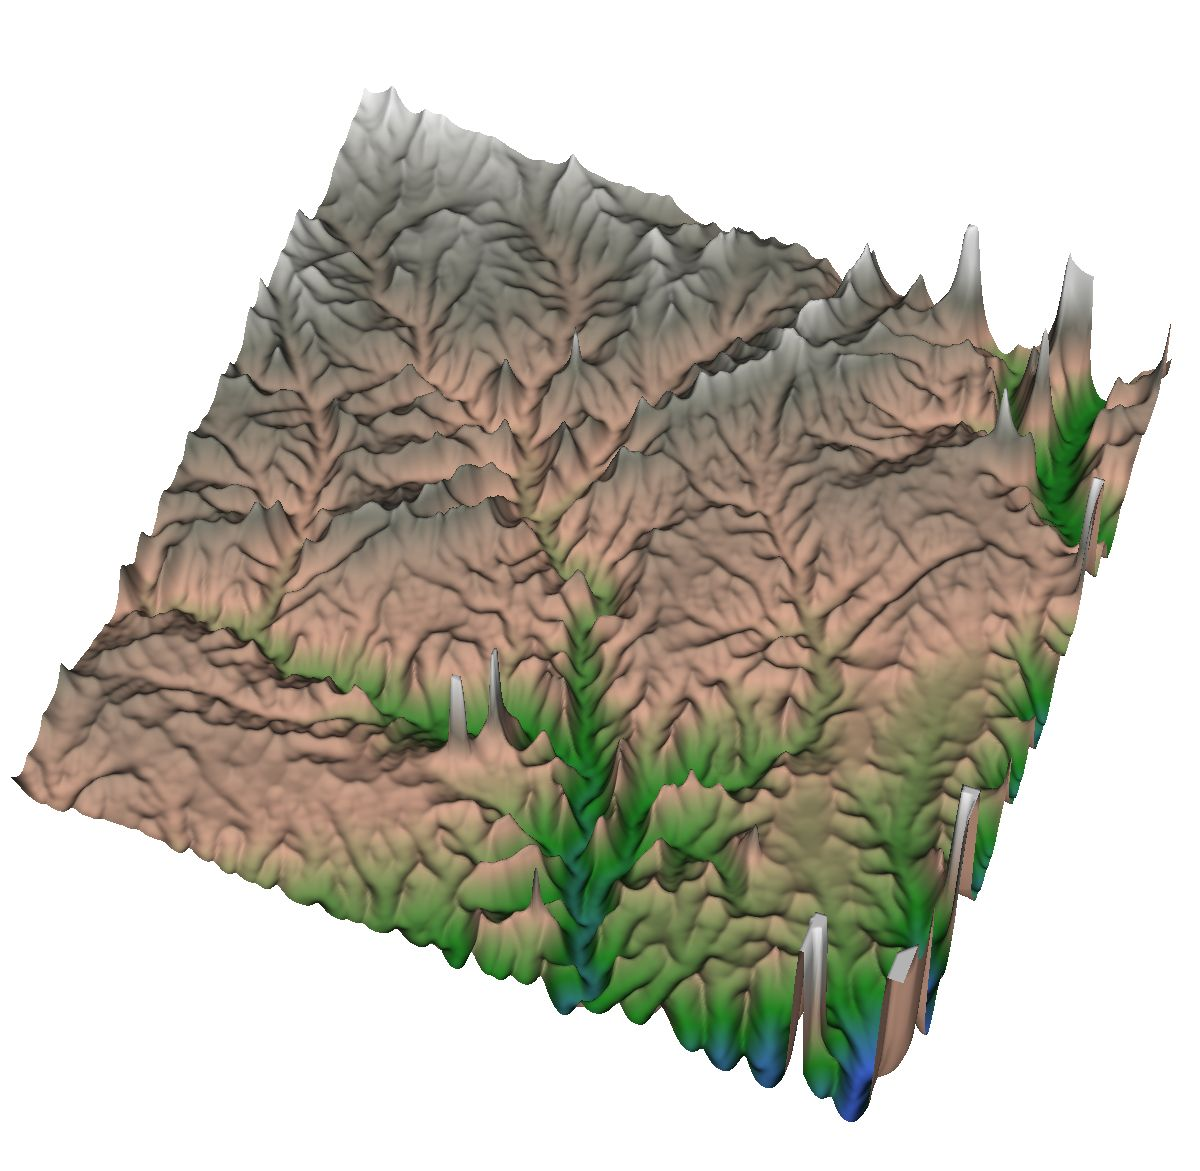
\includegraphics[width=0.99\linewidth]{images/W5_I10_T25.jpg} \\ \centering $\tau=25$, $w=5$, $k=10$ \end{minipage}
\end{center}
\caption[Regenerated terrains with lowest errors]{\label{figure:lowest_errors} The left image depicts the regenerated terrain with the lowest RMSE value, and the right image depicts the regenerated terrain with the lowest AHD error. The parameters responsible for the terrain are listed below the images. }
\end{figure}


The results for the accuracy tests are provided in Figure \ref{figure:results}. The left column of Figure \ref{figure:results} presents the data for the RMSE metric, and the data for the AHD is on the right. The error divisor for RMSE was the total elevation range of the original terrain, whereas the error divisor of AHD was the distance between pixel 0,0 and pixel $n$,$n$, the corners of the terrain. Since elevation is ignored for this divisor, it is possible for AHD error be greater than 1.0. 

$\tau$ values of 25 created considerably denser channel networks than $\tau$ values above 100, and so they are both more accurate and take considerably longer to calculate. The two channel networks can be seen in Figure \ref{figure:mtn2_original}. For reference, the maximum flow value for a pixel in the dataset is 102,245, and a threshold of 25 resulted in a channel network with $\approx19,000$ pixels, whereas a threshold of 100 resulted in a network of $\approx12,000$ pixels. Calculating the drill representation of a terrain with a flow threshold of 25 took approximately three minutes, and times decreased linearly with the increase in threshold value. The time for regenerating the terrain from the drill representation was quicker by approximately a factor of ten. It is important to note that optimization was not a focus at this time, and there exist many techniques that will be utilized in the future to reduce the time the algorithm takes.

There are several observations to be made regarding the accuracy data. The first is that, with ``good'' parameters (meaning none that create outliers in the error data), the accuracy is actually quite high with regard to both RMSE and AHD metrics, between 0.015 and 0.025. As with any algorithm, there is a trade-off between time and accuracy. The lower the threshold, the more pixels in the hydrography network, and so the slower the process, but the more accurate the results become. This is true in every case, and it makes intuitive sense. 

$\tau$ is the most influential parameter with regard to both metrics. 
This makes sense, since the drill is centered around the pixels of $N^{i}_{\tau}$. 
% shape calculation is constrained to pass through the center of $N^{i}_{\tau}$. 
Because AHD measures how close the channel networks are to one another, the more pixels there are in the channels the more likely it is that the channel networks overlap. By nature of the AHD, this will result in very low error. If the channel network is not dense enough, then the drill may not reach much of the terrain at all, and so the RMSE is also very much influenced by the value of $\tau$. More interesting is that the minimum RMSE occurred for when $w = 10$ and $k = 20$. It makes sense that a drill will need some influence over the area around the channel in order to reduce the RMSE, because without it there would be large areas of the terrain untouched by any drill, adding considerably to the overall error (that AHD would ignore). 

From a purely visual standpoint, many of the terrains pass the eyeball test. A side-by-side comparison of the terrains that represent the lowest error for each of the metrics is found in Figure \ref{figure:lowest_errors}. Notice is that the channels do seem to be somewhat wider in the RMSE winner, whereas they are more pointed, but areas of the terrain are missed by drills completely, in the AHD winner. Interestingly, the left image in Figure \ref{figure:lowest_errors} is one of the terrains we deem to be the most ``visually pleasing''. These often have higher $k$ and $w$ values, which may be a result of drills that flatten artifacts out of the terrain. This result demonstrates why, when choosing parameters for the drill operator, it is often smart to take both error metrics into account.


\section{Families of Functions for Drill Shape}
\label{section:FamiliesOfFunctions}

\begin{figure}[t]
  \caption[Graphical representations of drill shape functions.]{\label{figure:FamiliesOfFunctions} This figure shows graphical 2D examples of each of the families of functions making up several possible drill shapes.}
\end{figure}

\fbox{I will make a figure of the function families tested}


\begin{table}[t]
  \centering
  \begin{tabular}{ | c | c | c | c | }
    \hline
      & \textbf{AHD} & \textbf{RMSE} & \textbf{SSRMSE} \\
    \hline
    \textbf{Linear}&&&  \\
    \hline
    HILL1 & 0.0572 & 0.0700 & 0.1013 \\
    HILL2 & 0.1848 & 0.1564 & 0.0923 \\
    HILL3 & 0.0563 & 0.0394 & 0.0644 \\
    MTN1 & 0.0483 & 0.0517 & 0.1000 \\
    MTN2 & 0.0285 & 0.0141 & 0.0819 \\
    MTN3 & 0.0383 & 0.0379 & 0.0764 \\
    \hline
    \textbf{Quadratic}&&& \\
    \hline
    HILL1 & 0.0673 & 0.1230 & 0.1581 \\
    HILL2 & 0.1840 & 0.1581 & 0.1022 \\
    HILL3 & 0.0678 & 0.0965 & 0.1888 \\
    MTN1 & 0.0568 & 0.1364 & 0.2403 \\
    MTN2 & 0.0192 & 0.0184 & 0.1080 \\
    MTN3 & 0.0362 & 0.0771 & 0.1477 \\
    \hline
    \textbf{Cubic}&&&  \\
    \hline
    HILL1 & 0.2757 & 0.3413 & 0.3803 \\
    HILL2 & 0.1820 & 0.1674 & 0.0894 \\
    HILL3 & 0.2060 & 0.2412 & 0.3155 \\
    MTN1 & 0.6620 & 0.5032 & 0.1197 \\
    MTN2 & 0.0160 & 0.2521 & 0.1227 \\
    MTN3 & 0.5117 & 0.4783 & 0.1041 \\
    \hline
  \end{tabular}
  \caption[Minimum error values in tests for different drill shape function families.]{\label{table:FamiliesOfFunctionsResults} This table presents the minimum error found for each of RMSE, AHD, and SSRMSE metrics, divided by function family. The top third of the table refers to data for linear drill shapes, the middle third to quadratic drill shapes, and the bottom third to cubic drill shapes. The results for each of the six datasets found in Figure \ref{figure:SixDatasets} is reported.}
\end{table}

% Properly determining the drill shape can have a profound effect on the accuracy and flexibility of the operator. 
This section explores various drill shapes that can be used to represent the terrain surface.
The drill shape can be represented by any two-dimensional curve (not necessarily by a single-valued function). 
As a preliminary investigation into the effect of the drill shape, the following polynomial curves were investigated:
% This work investigates polynomial and logistic functions. 

\begin{itemize}
  \item Linear functions: Polynomials of degree one
  \item Quadratic functions: Polynomials of degree two
  \item Cubic functions: Polynomials of degree three
  \item Logistic functions
\end{itemize}

\fbox{FIX THE GRAPHIC}

\noindent Graphical examples of each of these families of functions can be seen in Figure \ref{figure:FamiliesOfFunctions}. Each family allows for arbitrarily steep slope (although slight modifications are required for vertical and negative slopes, though those can be incorporated with slight modifications to the fitting functions). 

A test was performed comparing the accuracy of each drill shape. Each test was a factorial experiment using the same three parameters described in Section \ref{section:DrillAccuracyTests} (channel network threshold, drill influence, cross-section size). For these experiments, the threshold was determined by the percentage of pixels to be extracted, and so $r$ was used as the third parameter in lieu of $\tau$. Using a percentage to define the extraction threshold provides a better idea of how much of the terrain is included in the channel network, and, more importantly, how many pixels are required to encode the terrain.

Three of the error metrics defined in Section \ref{section:DescriptionOfMetrics} were used for this test: AHD, RMSE, and SSRMSE. Beyond the fact that slope is an important terrain characteristic, the SSRMSE metric was included with AHD and RMSE (used in the test in Section \ref{section:DrillAccuracyTests}) in these tests because visual inspection of the results from Section \ref{section:DrillAccuracyResultsAndDiscussion} revealed that the peak areas between channels were pointed more than the original terrain. The slope-based metric will penalize this behavior more than RMSE.

Each possible drill function was tested in a factorial experiment. For each segment of the channel network, a single drill shape was determined (minimizing the number of fittings needed). Values up to 30 were tested for $r$ and $w$, and in the interest of limited time $k$ was set to the value of $w$. Logistic functions were immediately thrown away, as their results were incredibly bad. However, the results for the other three function families are presented in Table \ref{table:FamiliesOfFunctionsResults}.

Each of the values in the table is the minimum error found for each respective metric and dataset. Once again, the density of the pixels in the channel network is the most important parameter. In general, as the value of $r$ increases (with the number of drill operators), the accuracy of the representation increases as well. This is not always the case, but in most instances it is true. This means that $r$ can act as a tuning parameter for compression schemes, since it (more than the other parameters) controls the accuracy of the representation.

Somewhat surprisingly, the best results are almost universally within the linear group. A linear drill shape represented each terrain dataset within (approximately) 10\% error in each metric, with the exception of HILL2. The linear drill provided particularly good results for the more mountainous data in all three metric categories, and both HILL1 and HILL3 are adequately represented.

A closer inspection of HILL2 reveals that the dataset is very plateaued, and has few if any clearly defined channels. It is safe to say that, while the drill representation is capable of modeling hilly and plateaued terrains, it is better suited for more mountainous data, especially those with clearly defined channels. This may be due to the nature of the drill shape, or it might be due to the nature of the terrain. 
% method used to extract the channel network. 
On a flat or plateaued terrain, there are many instances in which determining neighbor flow requires tie-breaking procedures (as discussed in Section \ref{section:ChannelNetworkExtraction}). Major network extraction methods handle this differently, and so it is possible that, given a terrain with many ties among neighbors, two methods might produce radically different (and somewhat unstructured) networks. 
Extracted flow direction fields are not always intuitive and obvious on flatter terrain.

The results become increasingly worse as the degree of the polynomial family also increases. The cubic family is, for the most part, not a suitable representation of the surface. The quadratic family provides good-to-poor results, depending on the dataset. Once again, HILL2 is not modeled effectively, and MTN1 and HILL1 have poor RMSE results but good AHD results. This implies that the quadratic drills accurately model (and maintain) the channel networks, but fail to accurately model the data outside of them. 

Overall, the linear drill shape is adequate for modeling various terrain surfaces. The less detailed the surface, and the less clear the channel network to be extracted, the greater the chance for random outliers in error (such as HILL2). This suggests a procedure for trying multiple drill shapes for each channel individually, which is discussed in Section \ref{section:FutureWorkDrillOperator}.

% \section{Interpolating Drill Shapes}

In addition to testing these three drill shape families, the same test was run again using a procedure that assigned a single drill to an entire channel segment, rather than a single pixel. The drill shape was calculated at the first and last pixel of each segment, and for the pixels in between its shape was dynamically altered using linear interpolation. The results of this similar test were very close to the results listed in Table \ref{table:FamiliesOfFunctionsResults}, with 10\% for most data points and with no outliers. 

Because linear drill shape is the most accurate, and because it is equally as effective to assign a single dynamic drill shape to an entire channel, it is possible to store several pixels' worth of surface data very compactly by storing a single value for the start pixel, Freeman Chain Codes for the length of the channel, and two values for the drill shape polynomial. Therefore, a terrain can be effectively compressed. 

Finally, and perhaps most importantly, when a drill is assigned to and interpolated through a channel, and this process is consistent for all channels in the network, then local minima cannot appear in the regenerated terrain. This assumes that each segment travels downhill. Because the drill shape is monotonically increasing, the minimum of the terrain in any given local area must be the center of some drill, which is guaranteed to be at a higher elevation (lower priority) than its downstream neighbor in the channel network. This is true for all pixels all the way to the sink of the network, and therefore local minima cannot exist, satisfying one of the criteria of legal terrain generation.

\section{Compression Using the Drill Operator}
\label{section:TerrainCompression}

One of the natural applications of the drill representation is terrain compression. 
As discussed in Section \ref{section:TerrainDataCompression}, terrain data is often compressed with image compression techniques. These techniques achieve very good compression ratios and include progressive transmission which allows the user to provide either a data loss or a compression ratio threshold for near-lossless compression techniques.

However, these techniques ignore important terrain characteristics. For instance, the JPEG algorithm tends to blur sharp edges in images, thus inadvertently smoothing the image surface. The goal of this work is to preserve the important characteristics of the surface, specifically its hydrographical information. The drill representation seems a natural choice for this type of compression, since it is restricted to the pixels of the drainage network and mimics the physics of terrain generation. Therefore, this section presents a method for near-lossless terrain compression using the drill representation.

There are several considerations and sub-problems to tackle when determining how to store terrain data as compactly as possible. The first is to limit the encoding of a single drill. The second is to compress the locations of the drill, i.e. how to compress the drainage network. The final consideration is whether it is possible to allow for the user to determine a compression threshold, either with regard to storage or accuracy.

\subsection{The Compression Scheme}
\label{section:CompressionScheme}

\begin{figure}[t]
  \centering
  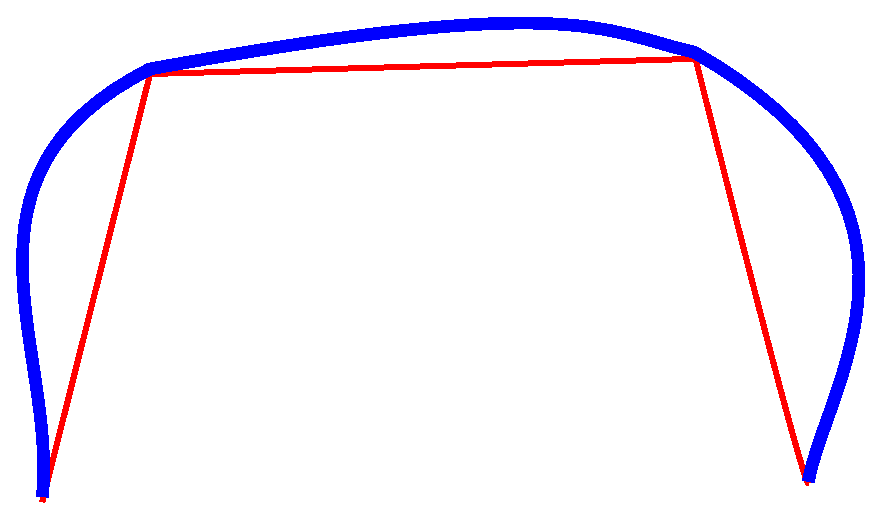
\includegraphics[width=0.6\textwidth]{images/LineGeneralization.eps}
  \caption[A simple example of line generalization.]{\label{figure:LineGeneralization}A simple example of line generalization, where a curve (blue) is represented by a working segment represented by 4 points along the curve connected by three line segments (red). Adding more points increases the accuracy of the generalization.}
\end{figure}


The steps to compressing the a terrain as a drill representation are as follows:

\begin{enumerate}
  \item Compress each segment of the drainage network using Freeman Chain Coding or line generalization.
  \item Encode each drill as an initial pixel and a drill shape.
  \item Compress the drill encoding.
  \item (Optional) Apply further compression techniques, such as 7Zip.
\end{enumerate}

As discussed in Section \ref{section:FamiliesOfFunctions}, a single drill can be encoded per segment of the channel network without significant loss of accuracy. In lieu of this, the various segments of the drainage network can be compressed using a scheme such as Freeman Chain Coding \cite{Freeman:1974:CPL:356625.356627} or line generalization \cite{Ramar72:Polygonalapproximation}. 

Freeman Chain Coding is a lossless method of compressing a line segment in an 8-directional system by storing the initial pixel location and then a chain of movement directions. The simplicity of the representation allows for additional compression, since each subsequent direction can be stored in 3 bits. In addition, taking advantage of the tendency for flows to travel in the same direction for long distances allows each segment to be compressed further by simple run length encoding, or more complex lossless compression.
 
Alternatively, line generalization is a lossy method of compressing a line segment by creating a current guess for the line, called the \textit{working segment}, initialized with the first and last pixel of the line.
% starting with the beginning and ending pixel of a segment and drawing a line between them. 
% This is the initial guess for the line segment. 
The furthest pixel from the working segment, using the 2-norm distance in pixel space, is then added to it, and a new guess is created with all the pixels in the working segment. This process is repeated until the desired accuracy or compression ratio is achieved. An example of this process can be seen in Figure \ref{figure:LineGeneralization}.

Since each line segment of the drainage network is now indexed in the encoding by its starting pixel, each drill can be stored in order of the index of the corresponding segment, and so only needs to be encoded as the shape. The drill encoding then becomes a $2 \times n$ matrix, where $n$ is the number of drills, and can be compressed with any lossless matrix compression scheme that is convenient. 

What is important to note is that Freeman Chain Coding is lossless, so if it is used along with a lossless compression of the drill matrix, the only accuracy lost by this scheme is found in the actual representation itself. To a degree, this is unnecessary since most terrain data is inherently inaccurate to begin with. However, by making the accuracy of the compression (either using lossless, or bounded with line generalization) adjustable, there is an additional level of control put in the hands of the user.

Once the compressed files are written, then can be compressed further with file archive problems such as 7Zip \cite{7z-Pavlov} and gzip. Both provide additional compression with minimal data loss.

\subsection{Results and Discussion of Compression Testing}

The six datasets shown in Figure \ref{figure:SixDatasets} were compressed using the scheme presented in Section \ref{section:CompressionScheme}, as well as image compression techniques PNG and JPEG, and archiving technique 7Zip.
For these tests, the drill was compressed by converting the ASCII data into binary data and storing the Freeman Chain Codes as an optimal series of 3-bit sequences.
The PNG and JPEG files were created using the respective MATLAB implementations, and the 7Zip files were created using the default Ubuntu 11.04 compression option. For the JPEG compression, the chosen bit-depth was 12 bits (because 8 was not enough to store the full range of elevations in the data).

The results of these compressions are presented in Table \ref{table:CompressionResults}.

\begin{table}[t]
  \centering
    \begin{tabular}{| l | l | l | l | l | l | l |}
      \hline
      & Original (Binary) & Original (ASCII) & Drill* & 7Zip & PNG & JPEG \\
      \hline
      HILL1 & 320.0 & 781.3 & 83.7 & 70.4 & 89.0 & 13.7 \\
      \hline
      HILL2 & 320.0 & 781.3 & 161.8 & 101.6 & 138.6 & 20.8 \\
      \hline
      HILL3 & 320.0 & 781.3 & 44.8 & 48.7 & 57.7 & 9.3 \\
      \hline
      MTN1 & 320.0 & 625.4 & 230.4 & 115.7 & 182.4 & 39.9 \\
      \hline
      MTN2 & 320.0 & 651.1 & 8.4 & 130.5 & 145.7 & 36.0 \\
      \hline
      MTN3 & 320.0 & 625.3 & 148.5 & 116.0 & 158.6 & 39.9 \\
      \hline
    \end{tabular}
  \caption[Results for compression scheme tests.]{\label{table:CompressionResults} The resulting files sizes (in KB) of files generated using the Drill, 7Zip, JPEG, and PNG compression schemes for each of the six datasets in Figure \ref{figure:SixDatasets}. Each file's original size is given, as well, for both binary and ASCII representations.}
\end{table}

The drill representation used for each dataset was chosen to be the smallest set of operators whose RMSE was below 5\%. The RMSE of each of the other representations was each 0\% (7Zip and PNG, which are lossless) or near 0\% (JPEG). For the drill representation, an additional compression step was applied, using the archive format 7Zip. The additional compression it provided was small, usually only one or two KBs.

The JPEG compression algorithm is very good. With minimal data loss (on a pixel-by-pixel elevation basis), JPEG outperformed all other compression schemes with regard to compression ratio. However, allowing for a 5\% RMSE, the drill compression is able to significantly outperform JPEG and all other schemes on the MTN2 dataset. As presented in Section \ref{section:FamiliesOfFunctions}, the drill is able to very tightly fit the MTN2 dataset, even with very few pixels included in the channel network. This allows for a very small representation to be compressed. 
If the set of operators that provided the smallest error is used, the MTN2 file size grows to \fbox{CHECK THIS FIGURE} 40.0 KB. This is still comparable to the JPEG scheme, and stores more information than JPEG while introducing very little error. 

The PNG scheme performs well for well-structured data with lots of flat areas (HILL1 and HILL3), due to the run-length nature of the scheme. 7Zip performs well for similar reasons, which is why it does not greatly benefit the drill scheme to use it as an additional step since the originally compressed file is very densely packed. 

Like many compression schemes, the drill is dependent upon the structure of the underlying data, most notably the extracted channel network. Improvements in the generalization of the channel network will improve compression ratios while continuing to limit error. As the results for MTN2 prove, it is possible for the drill to accurately and compactly represent a terrain dataset, and the compression scheme introduced in Section \ref{section:TerrainCompression} is feasible. 
% However, improvements to the drill fitting need to be made, whether they be better functions or a generalization of the extracted channel network, before the compression can be widely used for many datasets.
To make the scheme a practical reality, further development of drill fitting techniques is necessary, as well as a method for pruning and generalizing the channel network. Pruning can be accomplished by applying the Junction Point Balance scheme, discussed later in this thesis in Section \ref{section:JunctionBalance}.


% \section{Machining the Terrain}
% 
% \fbox{Chapter about machining}
% 
% 
% \section{Post-Processing the Terrain}
% 
% \fbox{Chapter about post-processing}


\section{Summary of the Drill Operator}
\label{section:FutureWorkDrillOperator}

Chapter \ref{chapter:DrillOperator} introduced the drill, a mathematical operator that can, with proper placement and shape fitting, represent a terrain dataset with little error (Section \ref{section:DrillAccuracyTests}). 
The drill operator mimics digging out the surface with a circular drill, and as such encodes more information than a simple height field or TIN representation. In addition to its ties to a physical process, the operator also allows for discontinuities to be encoded along the edges of the drill itself. This allows for the representation of cliff faces, such as along channel edges, something height fields and TINs are incapable of. Finally, when storing the drill location as a string of pixels (a channel segment), as discussed in Section \ref{section:FamiliesOfFunctions}, local minima on the surface are prevented.

Three families of drill shapes were tested to determine which represent the surface most accurately. The most accurate drill shape for most terrain datasets is the linear shape, with decreasing accuracy as the degree of the polynomial drill shape increases. Terrain with a higher level of detail around its extracted channels (i.e. mountainous terrain) is more suited for drill representations, but all terrains tested were adequately represented.

In addition, the drill operator was shown to be an effective mechanism for compressing terrain data, by storing the compressed channel network along with the encoded set of drill operators that represent the surface. The drill representation does not compress better than JPEG with regard to its compression ratio, but it stores more information and does not smooth the surface. Further improvements to the operator and the extraction of the channel network will greatly improve this compression scheme.

With a representation that can represent legal terrains, the capacity for more accurate data collection exists. This representation is still limited by its reliance on surface sampled elevation collection, as errors in the data are impossible to avoid. As terrain representations that can model more complex terrain formations compactly and robustly are developed, data collection techniques will be developed to take advantage of them. The drill operator is a step in that direction.

\section{Future Work for the Drill Operator}

There are several extensions to be made to the drill terrain representation. The first is the method in which the drill is fit to the surface can be extended in a variety of ways. Each channel segment of the terrain should not only have its own drill parameters, but its own drill shape altogether. In some areas, a linear drill is better suited to be fit to the terrain, whereas in others a quadratic would work better. Along those same lines, more drill shapes will be incorporated into the framework, including ones that do not follow the definition of a function (allowing for spherical drills for caves and overhangs). 

Does the order of the application of the drills matter? We can mimic the process of ``machining'' the terrain by applying broader drills first, and then refining the individual channels with finer and finer drills, like one would machine a piece of metal. Along similar lines, there are various post-processing techniques that can be applied to a regenerated terrain. For instance, the ODETLAP algorithm can smooth out outlier pixels while simultaneously filling in gaps. This would allow the use of fewer, more precise drills along the channel network without worrying about touching all parts of the terrain. However, ODETLAP can overly-smooth the surface, eliminating discontinuities. To minimize this issue, the drills can be re-applied to the terrain after the ODETLAP procedure.

In order to extend the drill operator, a method will be developed to quickly and accurately identify the optimal parameters for the drill fitting. As it stands, to find the representation with the minimum error, a brute force method was used. However, this can certainly be optimized. This thesis did not focus on temporal optimization of the algorithms, but this needs to be a focus moving forward in order to truly make the drill representation practical for data collection and compression.

% There are several ways in which the drill-fitting algorithm can be optimized. 
% The first is by storing channel segments as opposed to individual pixels, such as with Freeman chain codes \cite{Freeman:1974:CPL:356625.356627} or line generalization \cite{Ramar72:Polygonalapproximation}. If a channel network can be stored as a series of segments, with begin points, end points, and channel trajectories, along with a function of drill shape (allowing it to change along the length of the channel), then the overall storage of a terrain can be greatly reduced. Storing the channels as trajectories also allows for a post-processing step that forces the trajectories to be monotonic and decreasing, thus forcing a lack of local minima and allowing the drill operator to adhere to the second criterion for a ``legal terrain'' described in Section \ref{section:intro}.
% With regards to temporal optimization, the drill creation algorithm bottlenecks at the function fitting. A better method of function fitting may significantly improve the performance of the algorithm. Drills can be any shape, including simple cones, and have a width along the bottom. If the restriction that the drill shape functions be monotonic and increasing is lifted, a drill can be ball-shaped, which could model caves. These new parameters would allow for more customizability while maintaining a small memory footprint.

Two more operators will be added to the set of operators: the erosion operator, and the mudslide operator. The erosion operator picks up sediment from a high elevation and deposits it at a lower elevation, and the mudslide operator adds sediment to the terrain along a trajectory. Deeper mathematics of these three operators will be explored, including how to define the composition of two operations, and whether that creates a group over the composition operation.  
% In addition, 

We will investigate ways to post-process terrain to deal with small areas untouched by drill operations. A simple interpolation of the untouched areas may be a solution, or more sophisticated algorithms may be more useful. Also, the system, as it currently stands, has three user-defined parameters ($\tau$, $w$, and $k$). We will investigate ways to automatically determine the ideal value for each of these parameters before operation extraction, thus not relying on user knowledge to create the best representation. Ideally, every operator will store its own value for $k$.

Finally, terrain DEM data is isometric to greyscale image data. To date there has been a great deal of work done in applying algorithms for images to terrain, especially in the area of terrain compression. However, measuring error (or dissimilarity) using the plethora of image dissimilarity measures has not been explored to its fullest. In the future, the representations presented in this thesis will use more sophisticated image dissimilarity measures (such as a more direct application of the Earth Mover's Distance \cite{Rubner:2000:EMD:365875.365881}).
% \chapter{Measuring Terrain Distances}
\label{chapter:TerrainDistances}

% It is necessary to have 
A quantitative measure of the difference between two terrain datasets, specifically height fields, $T_{0}$ and $T_{1}$, is necessary 
in order to judge the accuracy of terrain compression schemes and data representations (such as the drill operator presented in Chapter \ref{chapter:DrillOperator}).
Therefore, the notion of \textit{terrain distance}, or \textit{terrain dissimilarity}, must be explored. This chapter will present a series of metrics that determine $d\left(T_{0}, T_{1}\right)$, the distance between two height field datasets.

\section{Description of Distance Metrics}
\label{section:DescriptionOfMetrics}

Traditional distance metrics for spatial datasets, such as terrain surfaces, include Root Mean Square Error (RMSE) and Slope Surface RMSE (SSRMSE). These metrics provide a measure of 
% precision and accuracy lost 
distance on a global scope but ignore what can be thought of as the ``important'' characteristics of terrain, such as the shape and behavior of watersheds and channel networks,
and have been used to judge the accuracy of compression schemes and terrain representations (Stookey et al. \cite{Stookey08parallelodetlap}).


RMSE measures the root of the average squared difference in heights across the terrain, as shown in Equation \ref{equation:RMSMetric}:

\begin{equation}
\label{equation:RMSMetric}
%   RMSE\left(T_{0}, T_{1}\right) = \sqrt{ \frac{\displaystyle\sum_{\textbf{p}\in T_{0}, \textbf{q} \in T_{1}}{ \left(\textbf{p}_{z} - \textbf{q}_{z} \right)^2 } }{ z_{max} - z_{min} } }
  RMSE\left(T_{0}, T_{1}\right) = \sqrt{ \frac{\displaystyle\sum_{\textbf{p}\in T_{0}, \textbf{q} \in T_{1}}{ \left(\textbf{p}_{z} - \textbf{q}_{z} \right)^2 } }{ |T_{0}| } }
\end{equation}

\noindent where $\bf{p}$ and $\bf{q}$ are corresponding pixels in two separate datasets, $\bf{p}_{z}$ and $\bf{q}_{z}$ are their elevation values, and 
% $z_{max}$ and $z_{min}$ are the maximum and minimum elevations of the pixels of $T_{0}$. 
$|T_{0}|$ is the number of pixels in $T_{0}$.
This metric provides a single global distance measurement when comparing two datasets.
% , normalized by the value range of the pixels in $T_{0}$.

% % % For any two sets of pixels (in this case, the sets of all pixels in the channel network of each terrain), AHD finds  the maximum value of the average of the infimum of the
% % % distances between the sets,
% % % % the average of the shortest distance between their pixels, 
% % % as shown in Equation \ref{equation:hausdorffAvg}:
% % % 
% % % \begin{equation}
% % % \label{equation:hausdorffAvg}
% % % d_{ave} \left( N^{T_{0}}_{\tau}, N^{T_{1}}_{\tau} \right) = \max\left\{ \overline{\inf_{\textbf{p}_{j} \in N^{T_{1}}_{\tau}, \textbf{p}_{i} \in N^{T_{0}}_{\tau}} d\left(\textbf{p}_{i}, \textbf{p}_{j}\right)}, \overline{\inf_{\textbf{p}_{i} \in N^{T_{0}}_{\tau}, \textbf{p}_{j} \in N^{T_{1}}_{\tau}} d\left( \textbf{p}_{i}, \textbf{p}_{j} \right)} \right\}
% % % \end{equation}
% % % 
% % % \noindent where $N^{T_{0}}_{\tau}$ is the $i^{th}$ pixel of the set of channel network pixels extracted using threshold $\tau$, and $d\left( \textbf{p}_{i}, \textbf{p}_{j} \right) $ is
% % % the Euclidean distance between pixels $\textbf{p}_{i}$ and
% % % $\textbf{p}_{j}$. 
% % %  This metric tends to give a much more
% % % realistic look at the channel networks' distances.
% 
% 

The slope surface RMSE metric measures the RMSE in the slope values at each pixel. To measure the SSRMSE, a slope surface is created by measuring the slope at each pixel. For each pixel $\textbf{p}_{i} = \left(x_{i}, y_{i}\right)$, the slope values is determined by Equation \ref{equation:PixelSlopeValue}:

\begin{equation}
\label{equation:PixelSlopeValue}
  \Delta_{xy} \left( \textbf{p}_{i} \right) = \dfrac{ |\left( \left( x_{i} + 1, y_{i}\right)_{z} - \left(x_{i} - 1, y_{i} \right)_{z} \right)| + |\left( \left( x_{i}, y_{i} + 1\right)_{z} - \left(x_{i}, y_{i} - 1 \right)_{z} \right)| }{2}
\end{equation}

SSRMSE measures the RMSE between the slope surfaces of $T_{0}$ and $T_{1}$, $S_{T_{0}}$ and $S_{T_{1}}$, respectively. This is described in Equation \ref{equation:SSRMSE}

\begin{equation}
\label{equation:SSRMSE}
  SSRMSE\left(T_{0}, T_{1}\right) = RMSE\left(S_{T_{0}}, S_{T_{1}}\right)
\end{equation}

Both of these metrics measure the global distances between two spatial datasets. However, when measuring the distance between two terrain datasets, it is often more appropriate to determine how dissimilar specific characteristics of the terrain are from one another.



The following two metrics take as input two channel networks
($N^{T_{0}}_{\tau}$ and $N^{T_{1}}_{\tau}$) and return the distance between
them. These metrics are used to help define the difference between the
terrains and thresholds from which the networks result. 
% % Since the metrics have been designed to 
% % take in any channel networks, comparisons between terrains
% % from simulation data (different time steps in the same sequence), between unrelated terrains, or even
% the same terrain with networks formed using different thresholds are possible.

% \subsection{Pixel-to-Pixel Correspondence Metric}
% \label{section:PixelToPixelCorrespondence}

The first metric is the pixel to pixel correspondence metric, described in equation \ref{equation:pix_dist}, in which
each pixel of $N^{T_{0}}_{\tau}$ is compared to each in $N^{T_{1}}_{\tau}$,
and two pixels are said to correspond if 
% their addresses have the same length (meaning 
they are each the same depth in their respective networks,
and their flow travels in the same direction. 
% I do not compare
% addresses directly because of potential inconsistencies in the
% labeling scheme applied to two similar but not identical networks.
% A slight change in threshold can cause a new, very small network to
% form elsewhere in the terrain, and as a result the ID system for the
% networks (Figure \ref{figure:addressingScheme}) is not comparable
% between thresholds, only a pixel's position within its own network.

\begin{align}
\label{equation:pix_dist}
  d_{pix} \left( N^{T_{0}}_{\tau}, N^{T_{1}}_{\tau} \right) = \dfrac{ \left| \left\{ \textbf{p}_{i} \  | \ \textbf{p}_{i} \rightarrow \textbf{p}_{j} \right\} \right| }{ \left| N^{T_{0}}_{\tau} \right|  }
\end{align}

\noindent where $\textbf{p}_{i} \in N^{T_{0}}_{\tau}\,$ and
$\textbf{p}_{j} \in N^{T_{1}}_{\tau}$ is its corresponding pixel (same x,
y coordinates in its respective terrain), and $\left| N^{T_{0}}_{\tau}
\right|$ is the total number of pixels compared, a normalizing
component.

% One major shortcoming of the pixel-to-pixel correspondence metric is that a small change in the network downstream of any pixel has the potential to drastically change the address assigned to the pixel. For this reason, the use of this metric should be limited to major channel networks after a pruning procedure has taken place. Thus, 
Pixels of similar networks correspond regarding their positions in the network, and thus this metric is a normalized count of the number of correlated pixels between two networks. This metric also inherently uses channel length as a measure of dissimilarity.

% \subsection{Hausdorff Distance Metrics}
% \label{section:HausdorffDistanceMetrics}

The second metric is an adaptation of the traditional \emph{Hausdorff distance} metric, defined in equation \ref{equation:hausdorff}.

\begin{align}
\begin{split}
\label{equation:hausdorff}
& d_{haus} \left( N^{T_{0}}_{\tau}, N^{T_{1}}_{\tau} \right) =  
\max \left\{ \sup_{ \textbf{p}_{i} \in N^{T_{0}}_{\tau} } \inf_{ \textbf{p}_{j} \in N^{T_{1}}_{\tau} } d\left( \textbf{p}_{i} \, \textbf{p}_{j} \right) \, \sup_{ \textbf{p}_{j} \in N^{T_{1}}_{\tau} } \inf_{ \textbf{p}_{i} \in N^{T_{0}}_{\tau} } d\left( \textbf{p}_{i} \, \textbf{p}_{j} \right) \right\}
%  \max\left\{ \overline{\inf_{\textbf{p}_{j} \in N^{T_{1}}_{\tau}, \textbf{p}_{i} \in N^{T_{0}}_{\tau}} d\left(\textbf{p}_{i}, \textbf{p}_{j}\right)}, \overline{\inf_{\textbf{p}_{i} \in N^{T_{0}}_{\tau}, \textbf{p}_{j} \in N^{T_{1}}_{\tau}} d\left( \textbf{p}_{i}, \textbf{p}_{j} \right)} \right\}
\end{split}
\end{align}

\noindent where $d\left( \textbf{p}_{i}, \textbf{p}_{j} \right) $ is
the Euclidean distance between pixels $\textbf{p}_{i}$ and
$\textbf{p}_{j}$. The Hausdorff distance metric is a measure over all of the pixels in each channel network. It is defined as the maximum distance  of the set of minimum distances between a pixel $\textbf{p}_{i}$ in $N^{T_{0}}_{\tau}$ and the pixels in $N^{T_{1}}_{\tau}$. However, due to the nature of the metric, it can lend too much weight to outliers. Therefore, a third metric has been produced.

For any two sets of pixels, the average Hausdorff metric finds the average of the shortest distance between their respective pixels, as shown in Equation \ref{equation:hausdorffAvg}:
%  the average Hausdorff distance metric, as described by Equation \ref{equation:hausdorffAvg}.

\begin{align}
\label{equation:hausdorffAvg}
\begin{split}
& d_{avg} \left( N^{T_{0}}_{\tau}, N^{T_{1}}_{\tau} \right) = 
% \max \left\{ \overline{ \inf_{\textbf{p}_{j} \in N^{T_{1}}_{\tau} \textbf{p}_{i} \in N^{T_{0}}_{\tau} } d\left( \textbf{p}_{i}, \textbf{p}_{j} \right) }, \overline{ \inf_{\textbf{p}_{i} \in N^{T_{0}}_{\tau}, \textbf{p}_{j} \in N^{T_{1}}_{\tau} } d\left( \textbf{p}_{i}, \textbf{p}_{j} \right) } \right\}
 \max\left\{ \overline{\inf_{\textbf{p}_{j} \in N^{T_{1}}_{\tau}, \textbf{p}_{i} \in N^{T_{0}}_{\tau}} d\left(\textbf{p}_{i}, \textbf{p}_{j}\right)}, \overline{\inf_{\textbf{p}_{i} \in N^{T_{0}}_{\tau}, \textbf{p}_{j} \in N^{T_{1}}_{\tau}} d\left( \textbf{p}_{i}, \textbf{p}_{j} \right)} \right\}
\end{split}
\end{align}

\noindent where 
$\textbf{p}_{i} \in N^{T_{0}}_{\tau}$ is the $i^{th}$ pixel of the set of channel network pixels 
of $T_{0}$ extracted using threshold $\tau$, $N^{T_{0}}_{\tau}$. The overline means ``mean value of''. 
It is important to note that AHD is limited to the channel networks of the terrain, whereas RMSE is applied globally. 
Limiting RMSE to only $N_{\tau}$ would not give an accurate picture of how close the terrains' hydrography networks are, 
since the network pixels are found by looking at the global flow pattern. Even if the elevations of the pixels in $N_{\tau}$ 
are comparable, it does not indicate that the overall terrain shape is similar. In addition, slight variations 
in the location of the pixels in $N_{\tau}$ would render RMSE unusable.

% \noindent or the maximum value of the average of the infimum of the
% distances between the sets. This metric tends to give a much more
% realistic look at the channel networks' distances, as it smooths out inaccurate distances created by outliers. 


The average Hausdorff distance provides a general picture of how close the pixels in $N^{T_{0}}_{\tau}$ are to those in $N^{T_{1}}_{\tau}$. It is important to note that this is a Euclidean metric, based on their exact positions in $\mathbb{R}^{3}$. All information regarding the geometry of the channel network (such as slope), meander, or flow is ignored. However, unlike the RMS Error metric, the average Hausdorff distance is a measurement of the geometric distance between only the pixels in the channel network, and thus it places emphasis on them and ignores the rest of the terrain. In this way, ``unimportant'' elevation information and outliers are not taken into account. By limiting the metric to pixels in the channel network, the geometry of the entire terrain is inherently incorporated but weighted by distance and contribution to the channel network.
% , because it is all data critical to the formation of the channel network, while focusing the metric on the important pixels.





\section{Finding an Optimal Flow Threshold}

Once a definition of the distance between two terrains has been determined, then an optimal threshold value that minimizes the distance between two terrains can be found. 
% 
% A good deal of work has been done with the intent of finding an \emph{optimal} flow accumulation value with which to threshold the flow accumulation matrix to extract the channel network. 
There have been attempts to use drainage density (a ratio of flow value to pixel watershed size) as a value to threshold instead of flow accumulation, while others have attempted to use local curvature or gradient values, as discussed in section \ref{section:ChoosingAFlowThreshold}. 


A simple brute force method will find this threshold among a set of terrains, by trying several different thresholds for the terrains in question and recording those that produce the smallest distances.
What is a more interesting challenge is finding the optimal threshold to apply to each terrain in a sequential series. 
If there are several terrains that belong to a series (such as time steps in an erosion simulation, or several regenerated terrains that had been compressed with various parameters), $\{ T_{i} \}$, finding an optimal threshold to compare their channel networks requires a degree of sequential coherence so that networks change smoothly as one moves from one terrain to another.
% 
% 
% It is clear that this is an interesting and important avenue of research. With this in mind, I introduce 
% Therefore, a method for finding the optimal flow threshold with which to compare two terrains, $T_{i}$ and $T_{j}$ in a sequence is introduced.
% representing sequential time steps, $D_{i}$ and $D_{j}$, in a series of datasets from our erosion simulation. This procedure is limited to this situation because of the limited nature of the metrics presented in section \ref{section:DescriptionOfMetrics}. Because they apply best when two terrains should match closely with only minute differences, comparing two sequential datasets is an ideal situation.
% This algorithm works best when the extracted channel networks are similar to one another, such as when testing the accuracy of a compression scheme.

Despite the fact that $T_{i}$ and $T_{j}$ are assumed to be similar, the extracted channel networks are very sensitive to small changes in the chosen threshold value. Given this, the same threshold cannot necessarily be applied to $T_{i}$ and $T_{j}$, as there is no guarantee that the result channel networks will resemble one another.
%  (ADD IMAGE)
Additionally, when measuring the dissimilarity between a decompressed terrain and its baseline, small elevation errors may result in the same threshold resulting in significantly different channel networks. Therefore, a method for choosing threshold values for each terrain is important. 
% For the time being, I restrict its use to a series of temporally adjacent terrains in a series of time steps.

A moving window algorithm that can use any of the metrics introduced in section \ref{section:DescriptionOfMetrics} to determine the threshold that minimizes the distance between $T_{i}$ and $T_{j}$ is shown in algorithm \ref{algorithm:idealThreshold}.

\begin{algorithm}[t]
\begin{algorithmic}
  \STATE $avg \gets 0$
  \STATE $nComparisons \gets 0$
    \FOR{$w_{cur} = t - \mbox{\em WINDOW} \to t + \mbox{\em WINDOW}$}
      \FOR{$\tau = \tau_{min} \to \tau_{max}$}
	  \STATE $dist \gets d\left( N^{t}_{\tau}, N^{w_{cur}}_{\tau} \right)$
	  \STATE $avg \gets avg + \tau * c\left( dist \right)$
	  \STATE $nComparisons \gets nComparisons + 1$
     \ENDFOR
  \ENDFOR
  \STATE $avg \gets avg / nComparisons$
  \STATE return $avg$
\end{algorithmic}
\caption[The moving window algorithm for finding the ideal threshold.]{\label{algorithm:idealThreshold} The moving window algorithm for finding the ideal threshold between two terrains by comparing its channel network with those of its neighbors. {\em WINDOW} is a constant window size, $d\left(N^{t}_{\tau}, N^{w_{cur}}_{\tau} \right)$ is the distance between channel networks $N^{t}_{\tau}$ and $N^{w_{cur}}_{\tau}$, $[ \tau_{min}$, $\tau_{max} ]$ is the range of threshold values we wish to test, and $c\left( dist \right)$ is a weight applied to the distance between networks. A window size of 2 worked well for a 10-terrain sequence, and for $c$, a weight of 1 is often sufficient.}
\end{algorithm}

This method is limited by the nature of the windowing algorithm. Possible thresholds are tested across neighbors, but the sequential coherence may be adversely affected by the neighbors' choice for its threshold. 
% This windowing algorithm was used to determine the optimal thresholds to use 

% \chapter{Using the Drill Operator}
\label{chapter:UsingTheDrillOperator}

The drill operator presented in chapter \ref{chapter:DrillOperator} provides a unique and novel method for representing the shape of a terrain surface. This chapter explores the operator's utility 
by presenting various enhancements, applications, and uses for the drill operator with regard to accurately and compactly representing terrain data.
% by presenting accuracy tests that show how closely the operator representation can mimic terrain data. These initial accuracy tests are followed by an in depth exploration of various expanded uses and applications of the drill operator.


\section{Initial Accuracy Trials}
\label{section:DrillAccuracyTests}

To determine the feasibility of representing terrain as drills, initial accuracy tests were performed to determine how closely the drill representation modeled the $400 \times 400$ mountainous dataset seen in Figure \ref{figure:mtn2_original}. All tests were performed in Ubuntu 11.04 with a quad-core AMD Phenom II X4 945 Processor, with 8GB of RAM. The code was written in MATLAB.

\subsection{Experimental Methodology}

The three parameters of the system, as described in Chapter \ref{chapter:DrillOperator}, are the threshold used to extract the original terrain's channel network $\tau$, the size of the cross section $w$, and the influence of a drill (size of the representative matrix) $k$. Each of 3 thresholds, 3 cross-section sizes, and 6 influence values were used to build regenerated terrains in the factorial experiment described in this section. 

For each set of parameter values, the total error between the generated terrain and the initial terrain was calculated using a measure for dissimilarity between the two sets.
These metrics take as input two channel networks
($N^{i}_{\tau}$ and $N^{j}_{\tau}$) and return the distance between
them.
 The two metrics used were the standard root mean squares error (RMSE) metric, and the averaged Hausdorff distance (AHD) metric as described in Section \ref{section:DescriptionOfMetrics}.
% by Stuetzle et al. \cite{stuetzle-TerrainDistances}, inspired by the shape analysis techniques discussed in Section \ref{section:ShapeAnalysisTechniques}.

It is important to note that AHD is limited to the channel networks of the terrain, whereas RMSE is applied globally. Limiting RMSE to only $N_{\tau}$ would not give an accurate picture of how close the terrains' hydrography networks are, since the network pixels are found by looking at the global flow pattern. Even if the elevations of the pixels in $N_{\tau}$ are comparable, it does not indicate that the overall terrain shape is similar. In addition, slight variations in the location of the pixels in $N_{\tau}$ would render RMSE unusable. Therefore, the results for both metrics are analyzed in context of their maximum error and what they mean from a physical standpoint.

\subsection{Results and Discussion of Initial Accuracy Trials}
\label{section:DrillAccuracyResultsAndDiscussion}

\begin{figure}
\begin{center}
  \begin{minipage}{0.49\linewidth}
     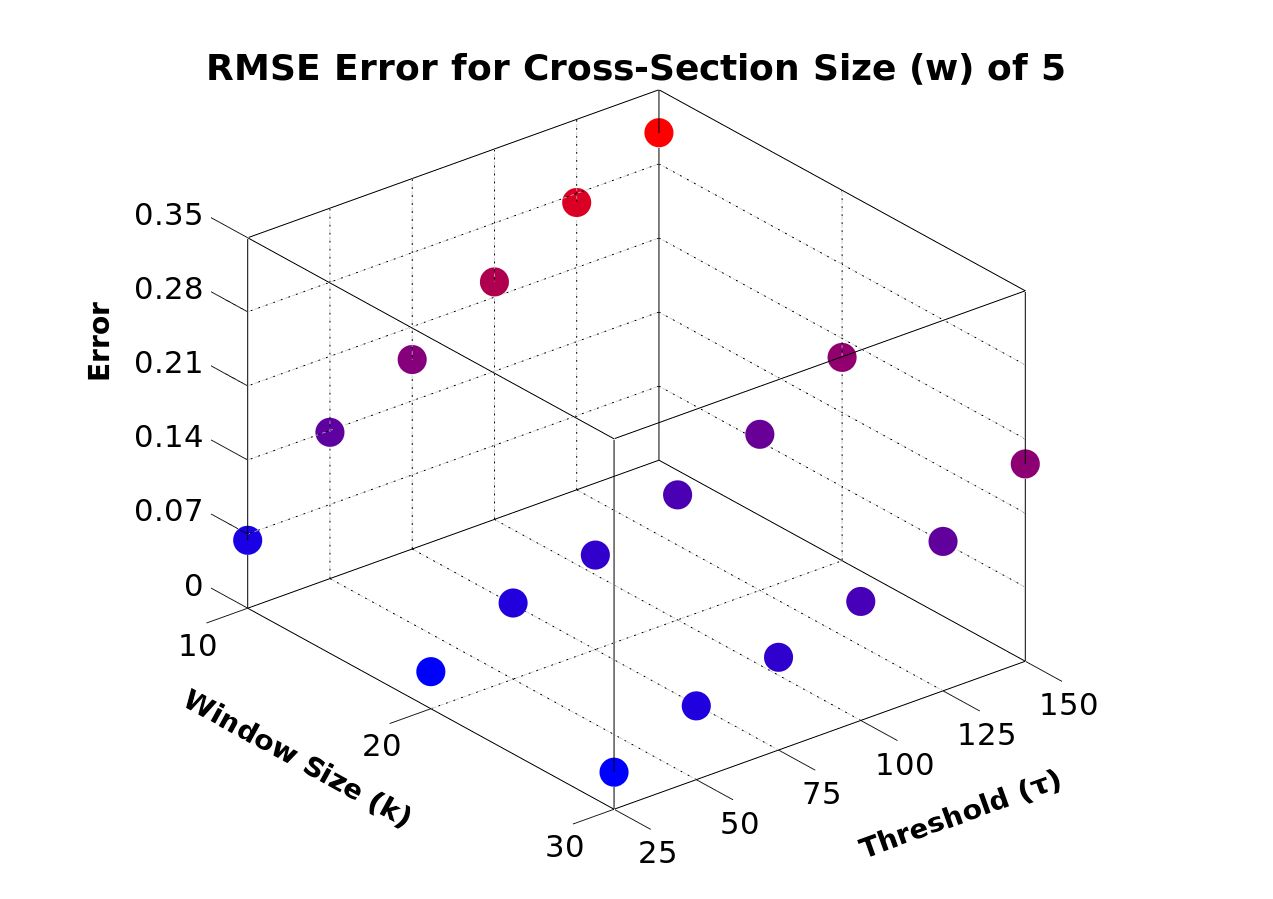
\includegraphics[height=0.25\textheight,width=0.99\linewidth]{images/RMSE_Graph_CS5.jpg} 

     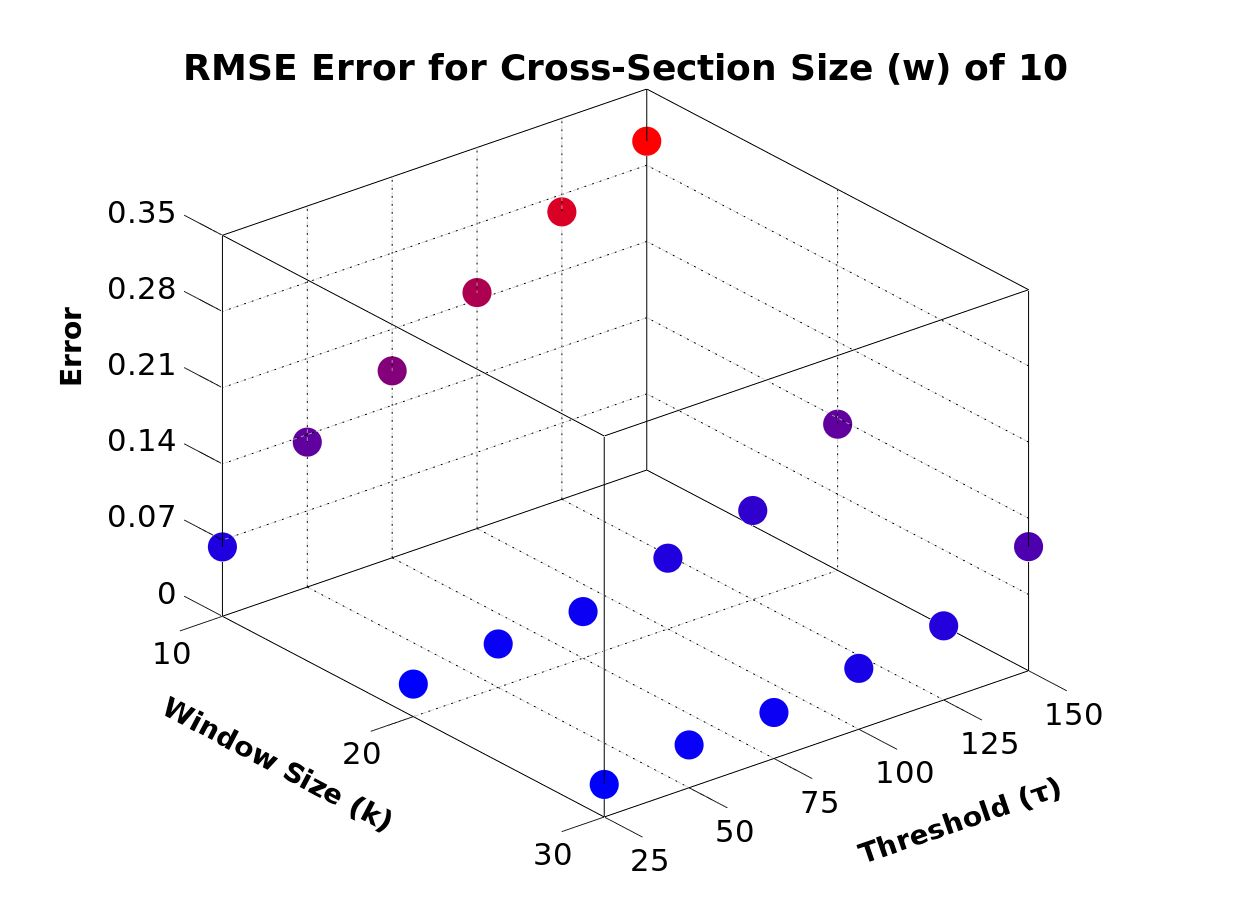
\includegraphics[height=0.25\textheight,width=0.99\linewidth]{images/RMSE_Graph_CS10.jpg}

     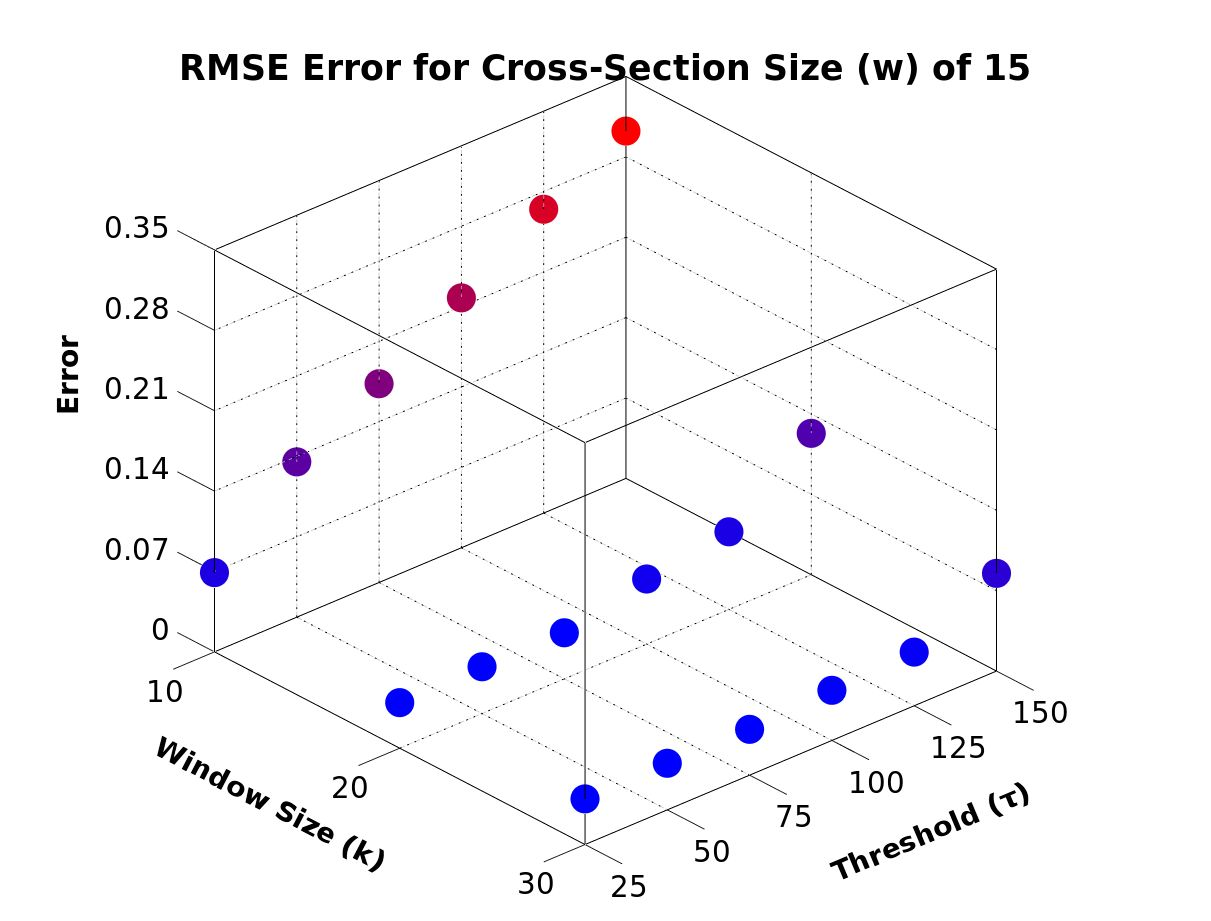
\includegraphics[height=0.25\textheight,width=0.99\linewidth]{images/RMSE_Graph_CS15.jpg}  
  \end{minipage}
  \begin{minipage} {0.49\linewidth} 
    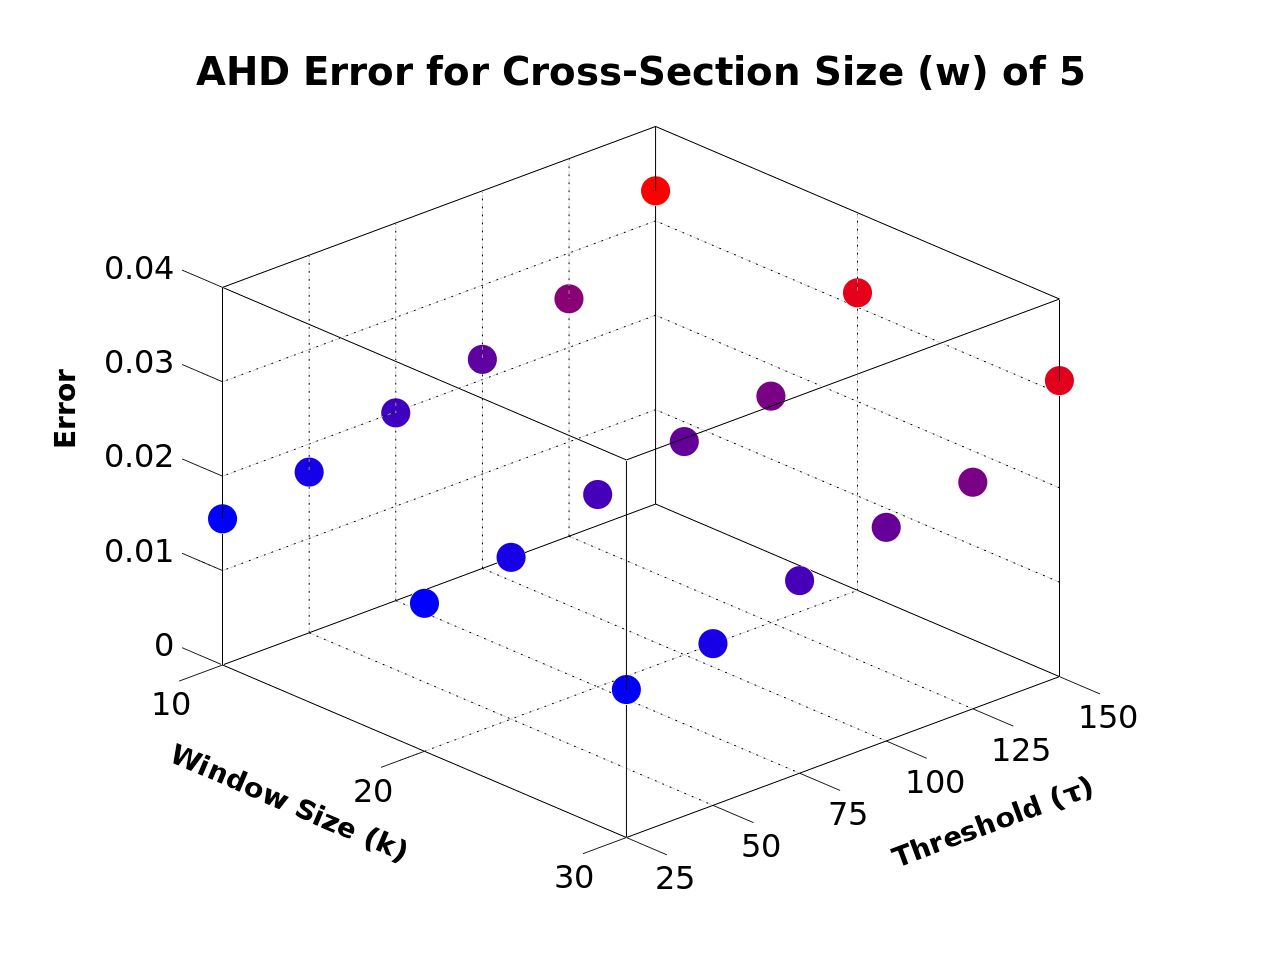
\includegraphics[height=0.25\textheight,width=0.99\linewidth]{images/AHD_Graph_CS5.jpg} 
 
    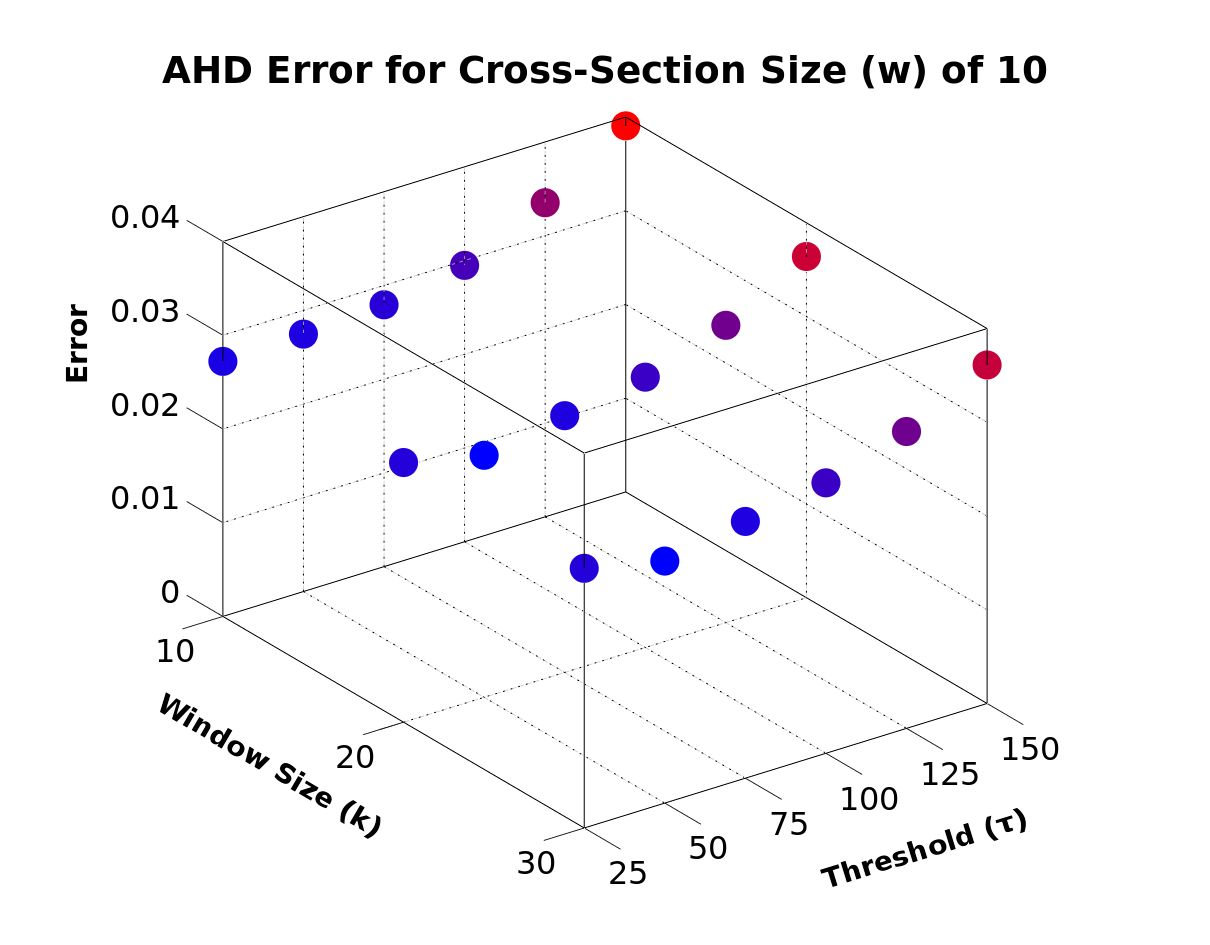
\includegraphics[height=0.25\textheight,width=0.99\linewidth]{images/AHD_Graph_CS10.jpg}

    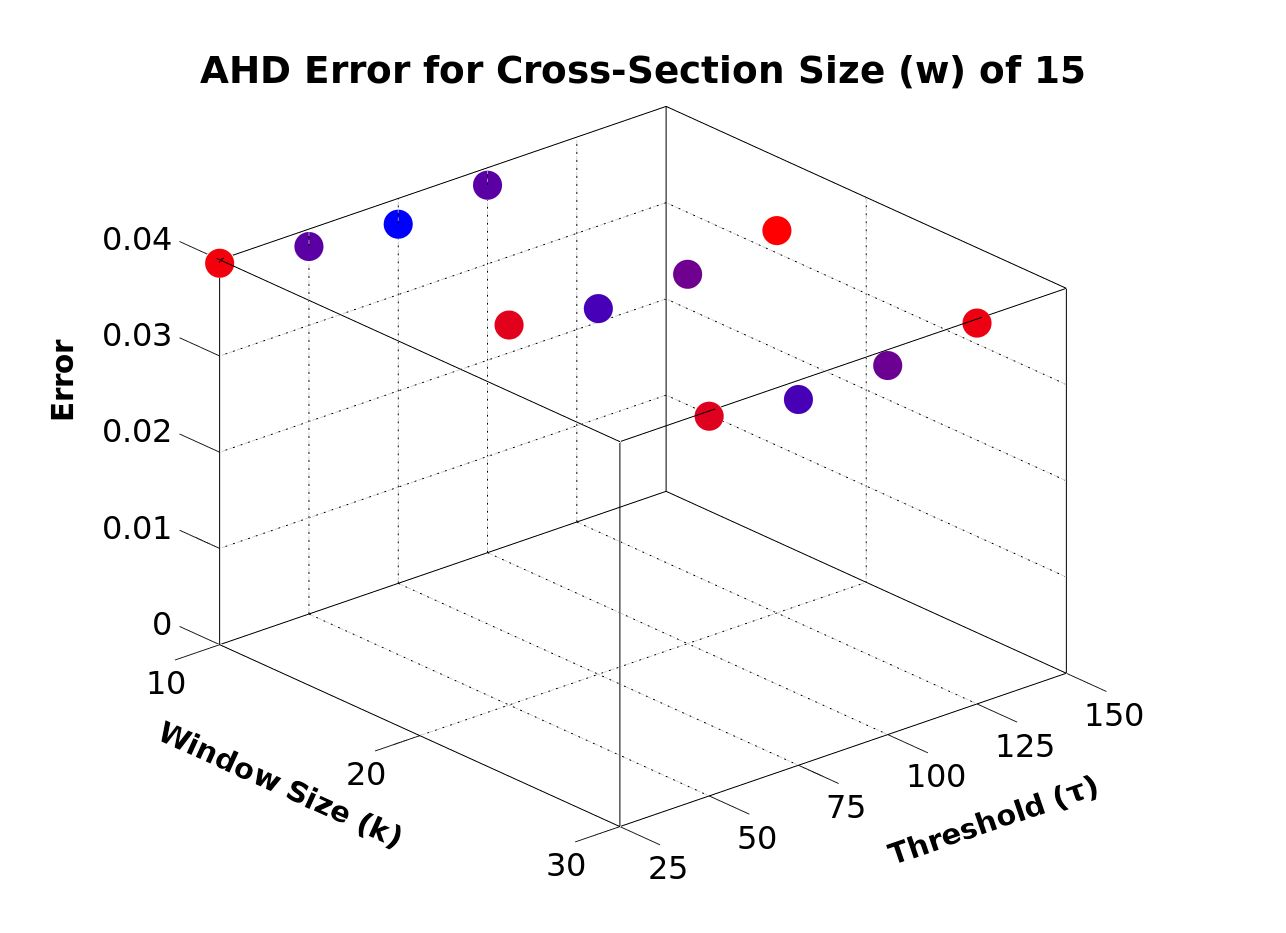
\includegraphics[height=0.25\textheight,width=0.99\linewidth]{images/AHD_Graph_CS15.jpg}
  \end{minipage}
\end{center}
\caption[The results for the concept tests for the drill operator]{\label{figure:results} The results of accuracy testing. The left column depicts the error measured using the RMSE metric, and the right column depicts error measured used the AHD metric. Each row shows a different value for the cross section window size (parameter $w$). Each metric's data is normalized. Red indicates high error, whereas blue indicates low error, local to each dataset.   }
\end{figure}


\begin{figure}[t]
\begin{center}
  \begin{minipage}{0.49\linewidth} 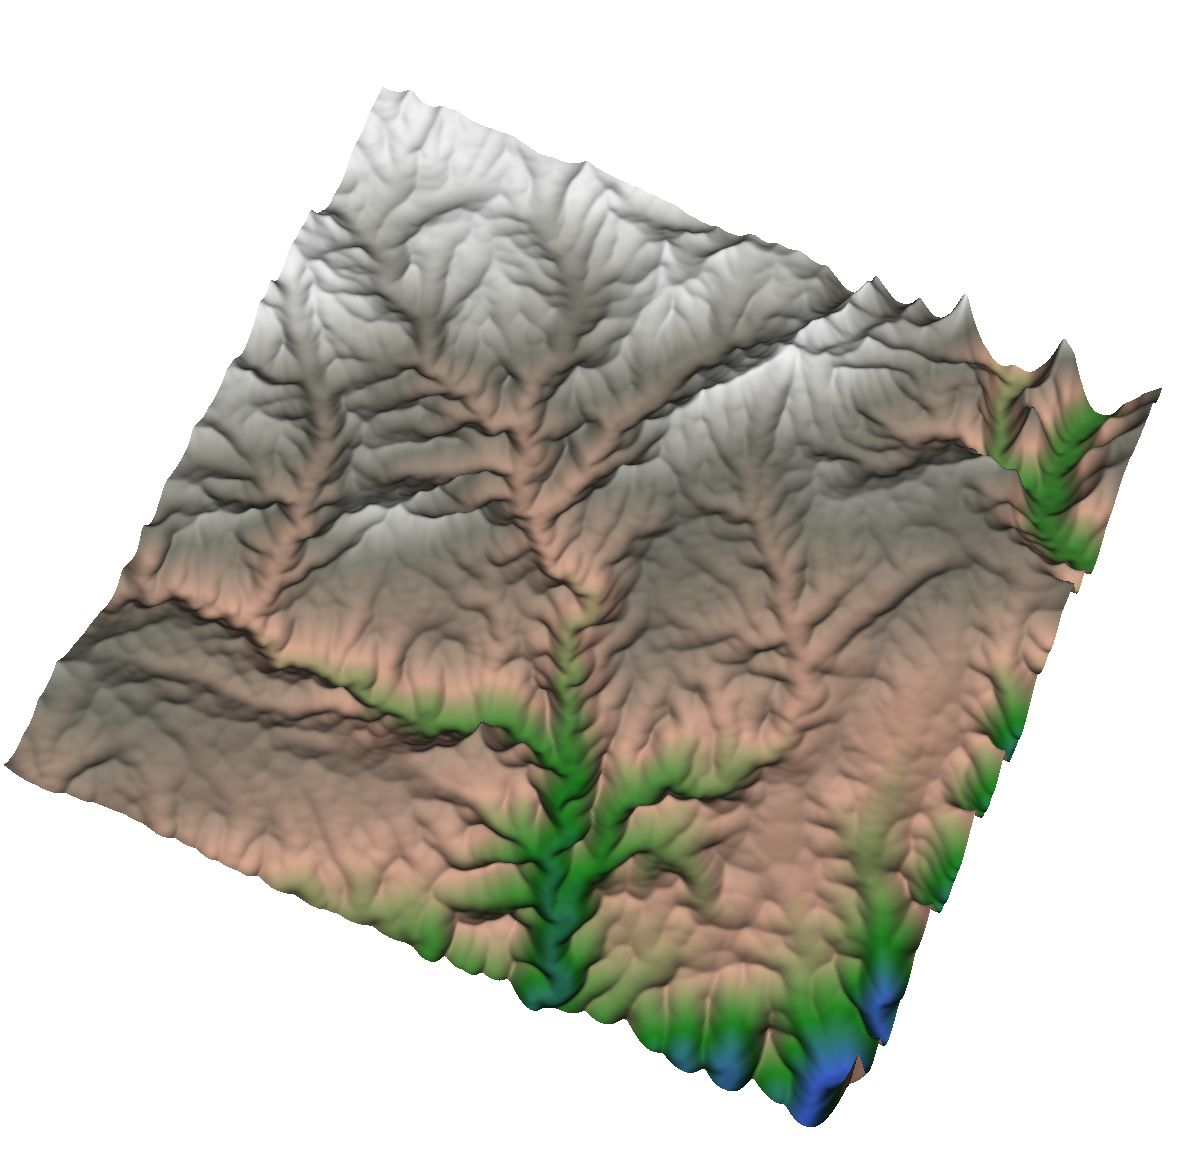
\includegraphics[width=0.99\linewidth]{images/W10_I20_T25.jpg} \\ \centering $\tau=25$, $w=10$, $k=20$ \end{minipage}
  \begin{minipage}{0.49\linewidth} 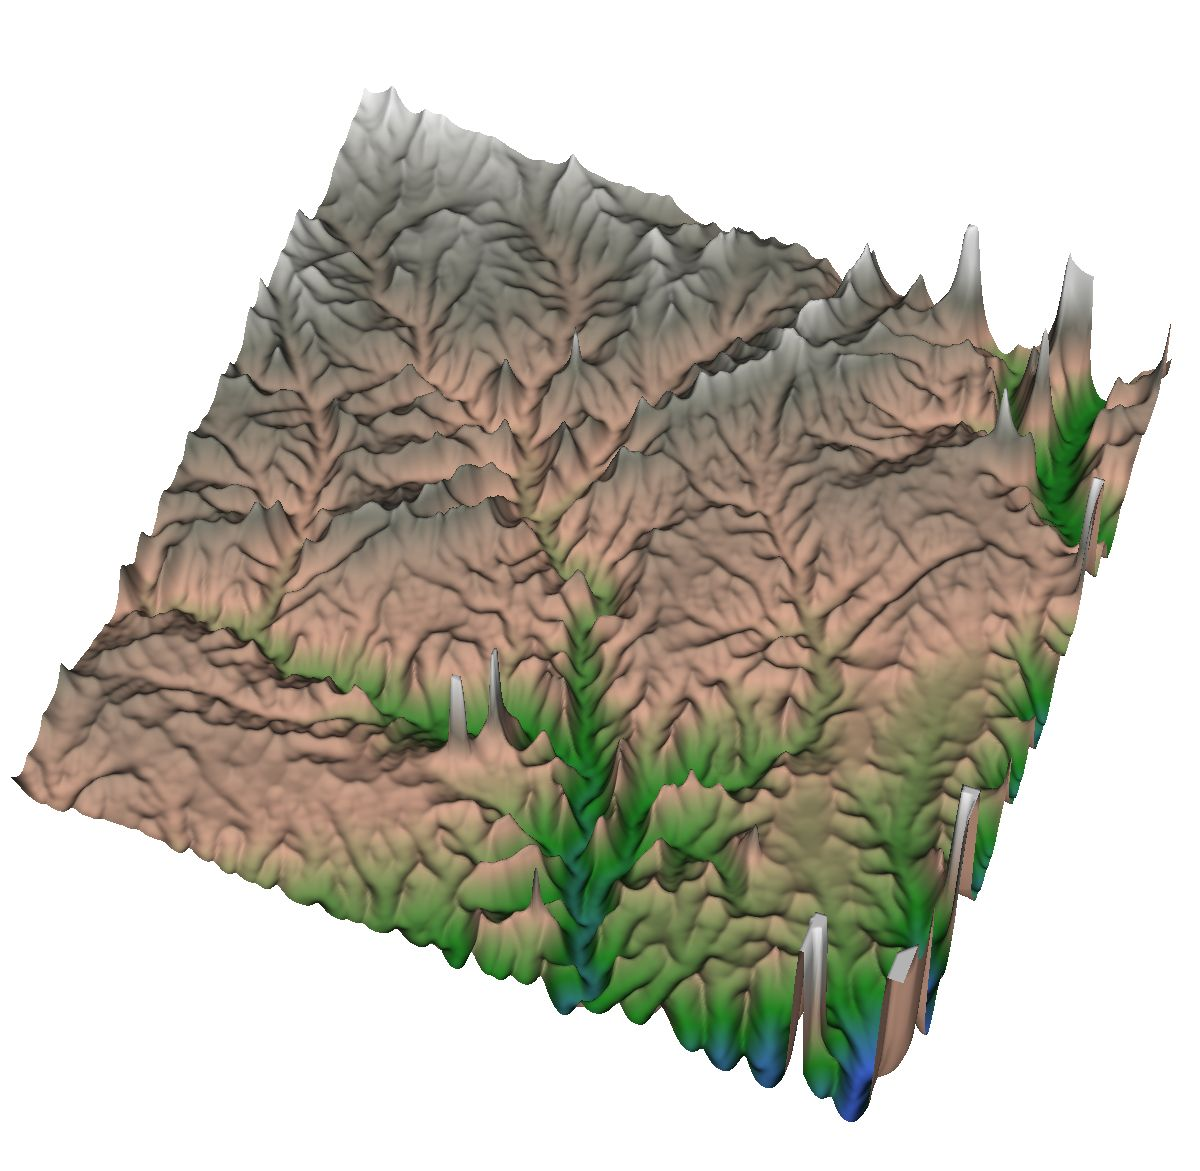
\includegraphics[width=0.99\linewidth]{images/W5_I10_T25.jpg} \\ \centering $\tau=25$, $w=5$, $k=10$ \end{minipage}
\end{center}
\caption[Regenerated terrains with lowest errors]{\label{figure:lowest_errors} The left image depicts the regenerated terrain with the lowest RMSE value, and the right image depicts the regenerated terrain with the lowest AHD error. The parameters responsible for the terrain are listed below the images. }
\end{figure}


The results for the accuracy tests are provided in Figure \ref{figure:results}. The left column of Figure \ref{figure:results} presents the data for the RMSE metric, and the data for the AHD is on the right. The error divisor for RMSE was the total elevation range of the original terrain, whereas the error divisor of AHD was the distance between pixel 0,0 and pixel $n$,$n$, the corners of the terrain. Since elevation is ignored for this divisor, it is possible for AHD error be greater than 1.0. 

$\tau$ values of 25 created considerably denser channel networks than $\tau$ values above 100, and so they are both more accurate and take considerably longer to calculate. The two channel networks can be seen in Figure \ref{figure:mtn2_original}. For reference, the maximum flow value for a pixel in the dataset is 102,245, and a threshold of 25 resulted in a channel network with $\approx19,000$ pixels, whereas a threshold of 100 resulted in a network of $\approx12,000$ pixels. Calculating the drill representation of a terrain with a flow threshold of 25 took approximately three minutes, and times decreased linearly with the increase in threshold value. The time for regenerating the terrain from the drill representation was quicker by approximately a factor of ten. It is important to note that optimization was not a focus at this time, and there exist many techniques that will be utilized in the future to reduce the time the algorithm takes.

There are several observations to be made regarding the accuracy data. The first is that, with ``good'' parameters (meaning none that create outliers in the error data), the accuracy is actually quite high with regard to both RMSE and AHD metrics, between 0.015 and 0.025. As with any algorithm, there is a trade-off between time and accuracy. The lower the threshold, the more pixels in the hydrography network, and so the slower the process, but the more accurate the results become. This is true in every case, and it makes intuitive sense. 

$\tau$ is the most influential parameter with regard to both metrics. 
This makes sense, since the drill is centered around the pixels of $N^{i}_{\tau}$. 
% shape calculation is constrained to pass through the center of $N^{i}_{\tau}$. 
Because AHD measures how close the channel networks are to one another, the more pixels there are in the channels the more likely it is that the channel networks overlap. By nature of the AHD, this will result in very low error. If the channel network is not dense enough, then the drill may not reach much of the terrain at all, and so the RMSE is also very much influenced by the value of $\tau$. More interesting is that the minimum RMSE occurred for when $w = 10$ and $k = 20$. It makes sense that a drill will need some influence over the area around the channel in order to reduce the RMSE, because without it there would be large areas of the terrain untouched by any drill, adding considerably to the overall error (that AHD would ignore). 

From a purely visual standpoint, many of the terrains pass the eyeball test. A side-by-side comparison of the terrains that represent the lowest error for each of the metrics is found in Figure \ref{figure:lowest_errors}. Notice is that the channels do seem to be somewhat wider in the RMSE winner, whereas they are more pointed, but areas of the terrain are missed by drills completely, in the AHD winner. Interestingly, the left image in Figure \ref{figure:lowest_errors} is one of the terrains we deem to be the most ``visually pleasing''. These often have higher $k$ and $w$ values, which may be a result of drills that flatten artifacts out of the terrain. This result demonstrates why, when choosing parameters for the drill operator, it is often smart to take both error metrics into account.


\section{Families of Functions for Drill Shape}
\label{section:FamiliesOfFunctions}

\begin{figure}[t]
  \caption[Graphical representations of drill shape functions.]{\label{figure:FamiliesOfFunctions} This figure shows graphical 2D examples of each of the families of functions making up several possible drill shapes.}
\end{figure}

\fbox{I will make a figure of the function families tested}


\begin{table}[t]
  \centering
  \begin{tabular}{ | c | c | c | c | }
    \hline
      & \textbf{AHD} & \textbf{RMSE} & \textbf{SSRMSE} \\
    \hline
    \textbf{Linear}&&&  \\
    \hline
    HILL1 & 0.0572 & 0.0700 & 0.1013 \\
    HILL2 & 0.1848 & 0.1564 & 0.0923 \\
    HILL3 & 0.0563 & 0.0394 & 0.0644 \\
    MTN1 & 0.0483 & 0.0517 & 0.1000 \\
    MTN2 & 0.0285 & 0.0141 & 0.0819 \\
    MTN3 & 0.0383 & 0.0379 & 0.0764 \\
    \hline
    \textbf{Quadratic}&&& \\
    \hline
    HILL1 & 0.0673 & 0.1230 & 0.1581 \\
    HILL2 & 0.1840 & 0.1581 & 0.1022 \\
    HILL3 & 0.0678 & 0.0965 & 0.1888 \\
    MTN1 & 0.0568 & 0.1364 & 0.2403 \\
    MTN2 & 0.0192 & 0.0184 & 0.1080 \\
    MTN3 & 0.0362 & 0.0771 & 0.1477 \\
    \hline
    \textbf{Cubic}&&&  \\
    \hline
    HILL1 & 0.2757 & 0.3413 & 0.3803 \\
    HILL2 & 0.1820 & 0.1674 & 0.0894 \\
    HILL3 & 0.2060 & 0.2412 & 0.3155 \\
    MTN1 & 0.6620 & 0.5032 & 0.1197 \\
    MTN2 & 0.0160 & 0.2521 & 0.1227 \\
    MTN3 & 0.5117 & 0.4783 & 0.1041 \\
    \hline
  \end{tabular}
  \caption[Minimum error values in tests for different drill shape function families.]{\label{table:FamiliesOfFunctionsResults} This table presents the minimum error found for each of RMSE, AHD, and SSRMSE metrics, divided by function family. The top third of the table refers to data for linear drill shapes, the middle third to quadratic drill shapes, and the bottom third to cubic drill shapes. The results for each of the six datasets found in Figure \ref{figure:SixDatasets} is reported.}
\end{table}

% Properly determining the drill shape can have a profound effect on the accuracy and flexibility of the operator. 
This section explores various drill shapes that can be used to represent the terrain surface.
The drill shape can be represented by any two-dimensional curve (not necessarily by a single-valued function). 
As a preliminary investigation into the effect of the drill shape, the following polynomial curves were investigated:
% This work investigates polynomial and logistic functions. 

\begin{itemize}
  \item Linear functions: Polynomials of degree one
  \item Quadratic functions: Polynomials of degree two
  \item Cubic functions: Polynomials of degree three
  \item Logistic functions
\end{itemize}

\fbox{FIX THE GRAPHIC}

\noindent Graphical examples of each of these families of functions can be seen in Figure \ref{figure:FamiliesOfFunctions}. Each family allows for arbitrarily steep slope (although slight modifications are required for vertical and negative slopes, though those can be incorporated with slight modifications to the fitting functions). 

A test was performed comparing the accuracy of each drill shape. Each test was a factorial experiment using the same three parameters described in Section \ref{section:DrillAccuracyTests} (channel network threshold, drill influence, cross-section size). For these experiments, the threshold was determined by the percentage of pixels to be extracted, and so $r$ was used as the third parameter in lieu of $\tau$. Using a percentage to define the extraction threshold provides a better idea of how much of the terrain is included in the channel network, and, more importantly, how many pixels are required to encode the terrain.

Three of the error metrics defined in Section \ref{section:DescriptionOfMetrics} were used for this test: AHD, RMSE, and SSRMSE. Beyond the fact that slope is an important terrain characteristic, the SSRMSE metric was included with AHD and RMSE (used in the test in Section \ref{section:DrillAccuracyTests}) in these tests because visual inspection of the results from Section \ref{section:DrillAccuracyResultsAndDiscussion} revealed that the peak areas between channels were pointed more than the original terrain. The slope-based metric will penalize this behavior more than RMSE.

Each possible drill function was tested in a factorial experiment. For each segment of the channel network, a single drill shape was determined (minimizing the number of fittings needed). Values up to 30 were tested for $r$ and $w$, and in the interest of limited time $k$ was set to the value of $w$. Logistic functions were immediately thrown away, as their results were incredibly bad. However, the results for the other three function families are presented in Table \ref{table:FamiliesOfFunctionsResults}.

Each of the values in the table is the minimum error found for each respective metric and dataset. Once again, the density of the pixels in the channel network is the most important parameter. In general, as the value of $r$ increases (with the number of drill operators), the accuracy of the representation increases as well. This is not always the case, but in most instances it is true. This means that $r$ can act as a tuning parameter for compression schemes, since it (more than the other parameters) controls the accuracy of the representation.

Somewhat surprisingly, the best results are almost universally within the linear group. A linear drill shape represented each terrain dataset within (approximately) 10\% error in each metric, with the exception of HILL2. The linear drill provided particularly good results for the more mountainous data in all three metric categories, and both HILL1 and HILL3 are adequately represented.

A closer inspection of HILL2 reveals that the dataset is very plateaued, and has few if any clearly defined channels. It is safe to say that, while the drill representation is capable of modeling hilly and plateaued terrains, it is better suited for more mountainous data, especially those with clearly defined channels. This may be due to the nature of the drill shape, or it might be due to the nature of the terrain. 
% method used to extract the channel network. 
On a flat or plateaued terrain, there are many instances in which determining neighbor flow requires tie-breaking procedures (as discussed in Section \ref{section:ChannelNetworkExtraction}). Major network extraction methods handle this differently, and so it is possible that, given a terrain with many ties among neighbors, two methods might produce radically different (and somewhat unstructured) networks. 
Extracted flow direction fields are not always intuitive and obvious on flatter terrain.

The results become increasingly worse as the degree of the polynomial family also increases. The cubic family is, for the most part, not a suitable representation of the surface. The quadratic family provides good-to-poor results, depending on the dataset. Once again, HILL2 is not modeled effectively, and MTN1 and HILL1 have poor RMSE results but good AHD results. This implies that the quadratic drills accurately model (and maintain) the channel networks, but fail to accurately model the data outside of them. 

Overall, the linear drill shape is adequate for modeling various terrain surfaces. The less detailed the surface, and the less clear the channel network to be extracted, the greater the chance for random outliers in error (such as HILL2). This suggests a procedure for trying multiple drill shapes for each channel individually, which is discussed in Section \ref{section:FutureWork}.

% \section{Interpolating Drill Shapes}

In addition to testing these three drill shape families, the same test was run again using a procedure that assigned a single drill to an entire channel segment, rather than a single pixel. The drill shape was calculated at the first and last pixel of each segment, and for the pixels in between its shape was dynamically altered using linear interpolation. The results of this similar test were very close to the results listed in Table \ref{table:FamiliesOfFunctionsResults}, with 10\% for most data points and with no outliers. 

Because linear drill shape is the most accurate, and because it is equally as effective to assign a single dynamic drill shape to an entire channel, it is possible to store several pixels' worth of surface data very compactly by storing a single value for the start pixel, Freeman Chain Codes for the length of the channel, and two values for the drill shape polynomial. Therefore, a terrain can be effectively compressed. 

Finally, and perhaps most importantly, when a drill is assigned to and interpolated through a channel, and this process is consistent for all channels in the network, then local minima cannot appear in the regenerated terrain. This assumes that each segment travels downhill. Because the drill shape is monotonically increasing, the minimum of the terrain in any given local area must be the center of some drill, which is guaranteed to be at a higher elevation (lower priority) than its downstream neighbor in the channel network. This is true for all pixels all the way to the sink of the network, and therefore local minima cannot exist, satisfying one of the criteria of legal terrain generation.

\section{Compression Using the Drill Operator}
\label{section:TerrainCompression}

One of the natural applications of the drill representation is terrain compression. 
As discussed in Section \ref{section:TerrainDataCompression}, terrain data is often compressed with image compression techniques. These techniques achieve very good compression ratios and include progressive transmission which allows the user to provide either a data loss or a compression ratio threshold for near-lossless compression techniques.

However, these techniques ignore important terrain characteristics. For instance, the JPEG algorithm tends to blur sharp edges in images, thus inadvertently smoothing the image surface. The goal of this work is to preserve the important characteristics of the surface, specifically its hydrographical information. The drill representation seems a natural choice for this type of compression, since it is restricted to the pixels of the drainage network and mimics the physics of terrain generation. Therefore, this section presents a method for near-lossless terrain compression using the drill representation.

There are several considerations and sub-problems to tackle when determining how to store terrain data as compactly as possible. The first is to limit the encoding of a single drill. The second is to compress the locations of the drill, i.e. how to compress the drainage network. The final consideration is whether it is possible to allow for the user to determine a compression threshold, either with regard to storage or accuracy.

\subsection{The Compression Scheme}
\label{section:CompressionScheme}

\begin{figure}[t]
  \centering
  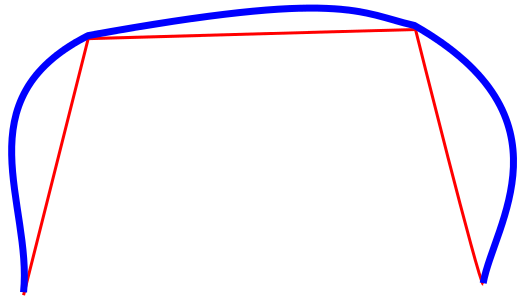
\includegraphics[width=0.6\textwidth]{images/LineGeneralization_cropped.png}
  \caption[A simple example of line generalization.]{\label{figure:LineGeneralization}A simple example of line generalization, where a curve (blue) is represented by a working segment represented by 4 points along the curve connected by three line segments (red). Adding more points increases the accuracy of the generalization.}
\end{figure}


The steps to compressing the a terrain as a drill representation are as follows:

\begin{enumerate}
  \item Compress each segment of the drainage network using Freeman Chain Coding or line generalization.
  \item Encode each drill as an initial pixel and a drill shape.
  \item Compress the drill encoding.
  \item (Optional) Apply further compression techniques, such as 7Zip.
\end{enumerate}

As discussed in Section \ref{section:FamiliesOfFunctions}, a single drill can be encoded per segment of the channel network without significant loss of accuracy. In lieu of this, the various segments of the drainage network can be compressed using a scheme such as Freeman Chain Coding \cite{Freeman:1974:CPL:356625.356627} or line generalization \cite{Ramar72:Polygonalapproximation}. 

Freeman Chain Coding is a lossless method of compressing a line segment in an 8-directional system by storing the initial pixel location and then a chain of movement directions. The simplicity of the representation allows for additional compression, since each subsequent direction can be stored in 3 bits. In addition, taking advantage of the tendency for flows to travel in the same direction for long distances allows each segment to be compressed further by simple run length encoding, or more complex lossless compression.
 
Alternatively, line generalization is a lossy method of compressing a line segment by creating a current guess for the line, called the \textit{working segment}, initialized with the first and last pixel of the line.
% starting with the beginning and ending pixel of a segment and drawing a line between them. 
% This is the initial guess for the line segment. 
The furthest pixel from the working segment, using the 2-norm distance in pixel space, is then added to it, and a new guess is created with all the pixels in the working segment. This process is repeated until the desired accuracy or compression ratio is achieved. An example of this process can be seen in Figure \ref{figure:LineGeneralization}.

Since each line segment of the drainage network is now indexed in the encoding by its starting pixel, each drill can be stored in order of the index of the corresponding segment, and so only needs to be encoded as the shape. The drill encoding then becomes a $2 \times n$ matrix, where $n$ is the number of drills, and can be compressed with any lossless matrix compression scheme that is convenient. 

What is important to note is that Freeman Chain Coding is lossless, so if it is used along with a lossless compression of the drill matrix, the only accuracy lost by this scheme is found in the actual representation itself. To a degree, this is unnecessary since most terrain data is inherently inaccurate to begin with. However, by making the accuracy of the compression (either using lossless, or bounded with line generalization) adjustable, there is an additional level of control put in the hands of the user.

Once the compressed files are written, then can be compressed further with file archive problems such as 7Zip \cite{7z-Pavlov} and gzip. Both provide additional compression with minimal data loss.

\subsection{Results and Discussion of Compression Testing}

The six datasets shown in Figure \ref{figure:SixDatasets} were compressed using the scheme presented in Section \ref{section:CompressionScheme}, as well as image compression techniques PNG and JPEG, and archiving technique 7Zip.
For these tests, the drill was compressed by converting the ASCII data into binary data and storing the Freeman Chain Codes as an optimal series of 3-bit sequences.
The PNG and JPEG files were created using the respective MATLAB implementations, and the 7Zip files were created using the default Ubuntu 11.04 compression option. For the JPEG compression, the chosen bit-depth was 12 bits (because 8 was not enough to store the full range of elevations in the data).

The results of these compressions are presented in Table \ref{table:CompressionResults}.

\begin{table}[t]
  \centering
  \begin{tabular}{ | c | c | c | c | c | c |}
    \hline
      & \textbf{Original File Size} & \textbf{Drill Representation} & \textbf{7Zip} & \textbf{JPEG} & \textbf{PNG} \\
    \hline
    HILL1 & 781.3 	& 83.7	& 70.4	& 13.7	& 89.0	\\
    HILL2 & 781.3 	& 161.8 & 101.6	& 20.8	& 138.6	\\
    HILL3 & 781.3 	& 44.8	& 48.7	& 9.3	& 57.7	\\
    MTN1 & 625.4 	& 230.4	& 115.7	& 39.9	& 182.4	\\
    MTN2 & 651.1 	& 8.4	& 130.5	& 36.0	& 145.7	\\
    MTN3 & 625.3 	& 148.5	& 116.0	& 39.9	& 158.6	\\
    \hline
  \end{tabular}
  \caption[Results for compression scheme tests.]{\label{table:CompressionResults} The resulting files sizes (in KB) of files generated using the Drill, 7Zip, JPEG, and PNG compression schemes for each of the six datasets in Figure \ref{figure:SixDatasets}. Each file's original size is given, as well.}
\end{table}

The drill representation used for each dataset was chosen to be the smallest set of operators whose RMSE was below 5\%. The RMSE of each of the other representations was each 0\% (7Zip and PNG, which are lossless) or near 0\% (JPEG). For the drill representation, an additional compression step was applied, using the archive format 7Zip. The additional compression it provided was small, usually only one or two KBs.

The JPEG compression algorithm is very good. With minimal data loss (on a pixel-by-pixel elevation basis), JPEG outperformed all other compression schemes with regard to compression ratio. However, allowing for a 5\% RMSE, the drill compression is able to significantly outperform JPEG and all other schemes on the MTN2 dataset. As presented in Section \ref{section:FamiliesOfFunctions}, the drill is able to very tightly fit the MTN2 dataset, even with very few pixels included in the channel network. This allows for a very small representation to be compressed. 
If the set of operators that provided the smallest error is used, the MTN2 file size grows to \fbox{CHECK THIS FIGURE} 40.0 KB. This is still comparable to the JPEG scheme, and stores more information than JPEG while introducing very little error. 

The PNG scheme performs well for well-structured data with lots of flat areas (HILL1 and HILL3), due to the run-length nature of the scheme. 7Zip performs well for similar reasons, which is why it does not greatly benefit the drill scheme to use it as an additional step since the originally compressed file is very densely packed. 

Like many compression schemes, the drill is dependent upon the structure of the underlying data, most notably the extracted channel network. Improvements in the generalization of the channel network will improve compression ratios while continuing to limit error. As the results for MTN2 prove, it is possible for the drill to accurately and compactly represent a terrain dataset, and the compression scheme introduced in Section \ref{section:TerrainCompression} is feasible. 
% However, improvements to the drill fitting need to be made, whether they be better functions or a generalization of the extracted channel network, before the compression can be widely used for many datasets.
To make the scheme a practical reality, further development of drill fitting techniques is necessary, as well as a method for pruning and generalizing the channel network. Pruning can be accomplished by applying the Junction Point Balance scheme, discussed later in this thesis in Section \ref{section:JunctionBalance}.


% \section{Machining the Terrain}
% 
% \fbox{Chapter about machining}
% 
% 
% \section{Post-Processing the Terrain}
% 
% \fbox{Chapter about post-processing}


\section{Summary of the Drill Operator}

Chapter \ref{chapter:DrillOperator} introduced the drill, a mathematical operator that can, with proper placement and shape fitting, represent a terrain dataset with little error (Section \ref{section:DrillAccuracyTests}). 
The drill operator mimics digging out the surface with a circular drill, and as such encodes more information than a simple height field or TIN representation. In addition to its ties to a physical process, the operator also allows for discontinuities to be encoded along the edges of the drill itself. This allows for the representation of cliff faces, such as along channel edges, something height fields and TINs are incapable of. Finally, when storing the drill location as a string of pixels (a channel segment), as discussed in Section \ref{section:FamiliesOfFunctions}, local minima on the surface are prevented.

Three families of drill shapes were tested to determine which represent the surface most accurately. The most accurate drill shape for most terrain datasets is the linear shape, with decreasing accuracy as the degree of the polynomial drill shape increases. Terrain with a higher level of detail around its extracted channels (i.e. mountainous terrain) is more suited for drill representations, but all terrains tested were adequately represented.

In addition, the drill operator was shown to be an effective mechanism for compressing terrain data, by storing the compressed channel network along with the encoded set of drill operators that represent the surface. The drill representation does not compress better than JPEG with regard to its compression ratio, but it stores more information and does not smooth the surface. Further improvements to the operator and the extraction of the channel network will greatly improve this compression scheme.

With a representation that can represent legal terrains, the capacity for more accurate data collection exists. This representation is still limited by its reliance on surface sampled elevation collection, as errors in the data are impossible to avoid. As terrain representations that can model more complex terrain formations compactly and robustly are developed, data collection techniques will be developed to take advantage of them. The drill operator is a step in that direction.

Future directions for the drill operator can be found in Section \ref{section:FutureWork}.
\chapter{Terrain Fingerprints}
\label{chapter:FingerprintingATerrain}




% FOOTNOTE THE ATTRIBUTIONS
\let\thefootnote\relax\footnote{Portions of this chapter previously appeared as: FIX \bibentry{stuetzle-TerrainDistances} }







% Chapter \ref{chapter:DrillOperator} presented the drill operator, a mathematical description of a terrain surface. Section \ref{section:TerrainDistances} presented a series of metrics used to measure the distance between two terrain datasets based solely on the shape of their extracted channel networks and the spatial positions of their elevation points. 
The idea that the underlying mathematics of a terrain surface can be used as an accurate representation of terrain will be taken one step further in this chapter by introducing a method for representing the terrain as a series of statistical descriptors, and using these descriptors to define another distance metric for measuring terrain dissimilarity.

This chapter presents the idea of the \emph{fingerprint} of a terrain $T$. A terrain's fingerprint is a set of characteristics 
% displayed by the terrain that are
 drawn from the hydrographic channel network that can be extracted from the terrain as described in Section \ref{section:ChannelNetworkExtraction}. 
% Once the terrain's channel network is identified, a series of statistical and geometric characteristics are extracted, making up the terrain's fingerprint. 
These characteristics describe a variety of aspects of the terrain including 
% channel shape, 
drainage density, flow pattern, and individual pixel importance.


% A fingerprint provides a 
% % mostly 
% unique 
% description of a terrain surface. One important application is the determination of a measure of dissimilarity between two terrains by assigning a quantity to the distance between their fingerprints. The typical methods for measuring terrain distance, as described in Section \ref{section:DescriptionOfMetrics}, fail to capture the local differences in terrain hydrography. These differences would provide a more localized error metric.
% Quantitative and qualitative comparison of this error makes possible deeper analysis of channel network evolution, as well as leads directly to more useful methods for choosing the flow threshold values used during channel network extraction, as discussed in Section \ref{section:ChoosingAFlowThreshold}.
% 
Fingerprints also provide insight into the behavior of water on the terrain, because they are determined by the terrain's channel network. Many applications rely on determining water flow on a surface, including flood planning and dam siting. 

\section{Pixel Identification}
\label{section:PixelIdentification}

Firstly, a method for identifying and categorizing the pixels in the extracted channel network, $N_{\tau}$, is necessary. For this purpose, each pixel $\textbf{p}_{i} \in N_{\tau}$ 
% belonging to the extracted channel network after thresholding the flow
%  with positive flow remaining 
in assigned a designation. A pixel can be designated with one of five categorizations based on the flow direction of it and any of its eight neighbors that also reside in the extracted channel network. The term ``neighbor'' as used in this designation is restricted to those pixels within the channel network:
%  (the term ``non-zero neighbor'' refers to neighbors in the channel network): 

\begin{itemize}
  \item Channel Start (S): All neighbors carry flow {\em away} from this pixel.
  \item Channel End (E): All neighbors carry flow {\em into} this pixel. %  At least one neighbor must be non-zero.
  \item Channel Junction (J): Flows to exactly one neighbor, while more than one neighbor contributes to this pixel's flow.
  \item Channel (C): Exactly one neighbor contributes to the pixel's flow, and this pixel contributes to exactly one neighbor.
%   \item Island (I): All neighboring pixels have flow lower than the threshold.
\end{itemize}

\noindent 
% Note that an effective flow threshold should provide a network with few, if any, I pixels, and only when using a flow accumulation algorithm that does not guarantee flow off the edge of the terrain. 
It is 
% also 
important to note that, when using a flow accumulation algorithm in which a pixel's entire flow is applied to a single neighbor (as opposed to using a fractional flow method), channels can not split. An example of a channel network with designated start, end, and junction points is found in figure \ref{figure:channelPoints}.

\begin{figure*}[t]
\centering
\begin{minipage}[b]{0.9\linewidth}
\begin{center}
\includegraphics[width=\linewidth]{images/RiverGraph2_crop.png}
\end{center}
\end{minipage}
\caption[Channel pixel assignment visualization]{\label{figure:channelPoints}The pixels that make up the channel network are labeled based on incoming and outgoing flow, starting from each channel end. S pixels are red, J pixels are green, and E pixels are yellow.}
\end{figure*}

A more formal definition of a channel \emph{segment} than the one presented in Chapter \ref{chapter:DrillOperator} is a set of pixels connecting an S to an E, an S to a J, a J to a J, or a J to an E. Segments will consist of exactly two S, E, or J pixels and a series of 0 or more 8-connected contiguous C pixels. A channel \emph{network} is defined as a series of connected segments. Each network can contain any number of S pixels but exactly one E pixel.

To each network within a terrain we assign an i.d. $i$, so a network in $T$ is $N^{i}_{\tau}$. An \emph{address} is assigned to each pixel \textbf{p} in $N^i_{\tau}$, designating in which $N^i_{\tau}$ it is found. The process of assigning addresses to pixels is a recursive tree traversal algorithm that begins at an E pixel and adds another level to the address whenever a J pixel is encountered, ending at an S pixel. An illustration of this addressing scheme is found in Figure \ref{figure:addressingScheme}, and the procedure can be found in Algorithm \ref{algorithm:addressingScheme}.

\begin{figure*}[t]
\centering
\begin{minipage}[b]{0.9\linewidth}
\begin{center}
\includegraphics[width=\linewidth]{images/network_diagram.pdf}
\end{center}
\end{minipage}
\caption[Pixel addressing visualization]{\label{figure:addressingScheme}The segments and nodes that compose each channel network on the terrain are consistently labeled, starting from each channel end. This graphic shows two examples of the labeling and addressing scheme.}
\end{figure*}

\begin{algorithm}[t]
assignPixelAddress( pixel \textbf{p}, address )
\begin{algorithmic}
  \STATE $newChannels \gets 0$
  \STATE $Pnbrs = getPNeighbors( \textbf{p} )$ 
  \IF{ $Pnbrs > 1$ }
    \STATE $address.pushOntoBack( newChannels )$
    \STATE $newChannels \gets newChannels + 1$
  \ENDIF
  \FOR{ $i \in Pnbrs$ }
    \STATE $assignPixelAddress( i, address )$
    \IF{$ Pnbrs > 1$ }
      \STATE $address.popOffBack$
      \IF{$i + 1 < Pnbrs$}
	\STATE $address.pushOntoBack( newChannels )$
	\STATE $newChannels \gets newChannels + 1$	
      \ENDIF
    \ENDIF
  \ENDFOR
\end{algorithmic}
\caption[Pixel addressing algorithm]{\label{algorithm:addressingScheme}The method used to determine the address of each pixel in the channel network. The function $assignPixelAddress(\textbf{p}, address)$ is recursively called for each pixel in a depth first fashion, assigning the current address (a string of integers) to the current pixel, and then adjusting the back value of the address string for each additional neighbor of the pixel. Note that $getPNeighbors$ is a subroutine that returns only neighboring pixels in the channel network.}
\end{algorithm}

Once the pixels of the channel network have been identified, and their addresses have been assigned, the fingerprint may be calculated.



\section{Fingerprint Characteristics}
\label{section:FingerprintCharacteristics}

% There are two distinct types of fingerprint characteristics. The first is those that require a ``baseline'' terrain, $T_{0}$, to use as time 0 for a series of temporally evolving terrains. These characteristics are computed using erosion depth at each pixel, which can only be accurately obtained by comparing to a matching baseline, pre-eroded terrain. An example of a dataset that matches this description are those that are generated by the erosion computer simulation presenting in section \ref{section:ErosionSimulation}. The second type of characteristic is one which can be computed on any individual terrain. These data are generally easier to find, and are represented in this work by those in figure \ref{figure:SixDatasets}.

The three characteristics that comprise terrain fingerprints are
% channel width, channel depth, 
meander, pixel load, and junction balance. This section describes these characteristics in detail. Each characteristic is represented by an $X \times Y$ sparse matrix of values. All pixels not part of the extracted channel network contain values of 0. 
% 
It is critical to remember that each of the fingerprint characteristics discussed in this section are sensitive to small changes in the flow threshold values used to obtain the channel network. For this reason, the threshold for all channel networks used in this section is constant, a flow accumulation value of 160,
as seen in Figure \ref{figure:ChannelNetwork_GlobalThreshold}.

% \subsection{Channel Depth and Width}
% \label{section:ChannelDepthAndWidth}
% 
% The two terrain characteristics that require a baseline terrain for calculation are channel depth and channel width. These provide for a pixel-by-pixel cross section of the channels formed through the evolution of the terrain under erosion conditions. Channel depth is the simpler of the two. To compute, a difference field is calculated, which is simply the difference in elevation between $D_{0}$ and time step in question, $T_{t}$. Figure \ref{figure:ThreeTimeStepsWithDepthsAndWidths} shows a series of three time steps, at 1 minute, 5 minutes, and 9 minutes of an erosion simulation, as well as the corresponding depth fields.
% 
% % Figure of three time steps and their erosion depths
% \begin{figure*}[t]
% \centering
% \begin{minipage}{0.9\linewidth}
% \begin{tabular}{@{}r@{}|@{}c@{}|@{}c@{}|@{}c@{}|}
% Time~ & Terrain & Channel Depth & Channel Width \\
% \hline
% \begin{sideways}
% \begin{large}~~~~~1:00~~~~~\end{large}
% \end{sideways}
% ~
% &
%   \begin{minipage}[b]{0.32\linewidth}
%   \begin{center}
%   \includegraphics[height=0.13\textheight]{images/ErodedTerrain_TimeStep1.png} \\
%   \end{center}
%   \end{minipage}
% &
%   \begin{minipage}[b]{0.32\linewidth}
%   \begin{center}
%   \includegraphics[height=0.13\textheight]{images/StatisticsTerrain1_ChannelDepth.jpg} \\
%   \end{center}
%   \end{minipage}
% &
%    \begin{minipage}[b]{0.32\linewidth}
%   \begin{center}
%   \includegraphics[height=0.13\textheight]{images/StatisticsTerrain1_ChannelWidth.jpg} \\
%   \end{center}
%   \end{minipage}
% \\ \hline
%   %
% \begin{sideways}
% \begin{large}~~~~~5:00~~~~~\end{large}
% \end{sideways}
% ~
% &
%   \begin{minipage}[b]{0.32\linewidth}
%   \begin{center}
%   \includegraphics[height=0.13\textheight]{images/ErodedTerrain_TimeStep5.png} \\
%   \end{center}
%   \end{minipage}
% &
%   \begin{minipage}[b]{0.32\linewidth}
%   \begin{center}
%   \includegraphics[height=0.13\textheight]{images/StatisticsTerrain5_ChannelDepth.jpg} \\
%   \end{center}
%   \end{minipage}
% &
%    \begin{minipage}[b]{0.32\linewidth}
%   \begin{center}
%   \includegraphics[height=0.13\textheight]{images/StatisticsTerrain5_ChannelWidth.jpg} \\
%   \end{center}
%   \end{minipage}
% \\ \hline
% \begin{sideways}
% \begin{large}~~~~~9:00~~~~~\end{large}
% \end{sideways}
% ~
% &
%   %
%   \begin{minipage}[b]{0.32\linewidth}
%   \begin{center}
%   \includegraphics[height=0.13\textheight]{images/ErodedTerrain_TimeStep9.png} \\
%   \end{center}
%   \end{minipage}
% &
%   \begin{minipage}[b]{0.32\linewidth}
%   \begin{center}
%   \includegraphics[height=0.13\textheight]{images/StatisticsTerrain9_ChannelDepth.jpg} \\
%   \end{center}
%   \end{minipage}
% &
%    \begin{minipage}[b]{0.32\linewidth}
%   \begin{center}
%   \includegraphics[height=0.13\textheight]{images/StatisticsTerrain9_ChannelWidth.jpg} \\
%   \end{center}
%   \end{minipage}
% \\ \hline
% \end{tabular}
% \end{minipage}
% %
% \caption[Channel depth and width visualization]{\label{figure:ThreeTimeStepsWithDepthsAndWidths}Three separate time steps of an erosion simulation. The geometry is a levee with a 5:1 slope, as seen in the left column. The center column displays a visualization of the depth at each pixel on the terrain, ranging from blue (little erosion depth) to red (significant erosion depth). The right column displays a visualization of the channel width field, ranging from blue (small width) to red (wide channels).}
% \end{figure*}
% 
% % Early in the simulation (time step 1:00) the erosion depth is scattered across the entire terrain, but as time passes it becomes much more localized to the channels that formed along the levee's downslope. Observe that very clear and well defined channel form as time passes. By the end of the simulation, it is possible to determine not only the boundaries of the channels, but also the deepest pixels, as well as some geometric properties. For instance, at the 9:00 mark, there are two major channels that have formed, one to the right and one to the left. However, the right channel flows around an uneroded plateau area, the dark blue patch just below the dark red area. This indicates a split in the flow of water.
% 
% Channel width is calculated for every pixel in the terrain, resulting in a channel width field in which every pixel is assigned a width value. Those pixels not in the channel network are assigned a value of 0. Width is calculated for a pixel \textbf{p} by determining the direction of flow from \textbf{p}, and walking along the terrain in each perpendicular (2D) direction until reaching either a pixel which has experienced no erosion, or until the walk is no longer uphill. In essence, this measures the distance one has to walk along the terrain until he is no longer walking uphill an eroded channel. It is important to note that the algorithm relies on the assumption that the channel pixels are the deepest pixels in the channel (because otherwise walking uphill would make no sense). This is an accurate assumption because, if it was not the case that the channel pixels were the lowest in a channel, then there would be pixels that the channel pixels would provide flow for, and thus there would be pixels with greater flow values. The procedure for calculation is described in Algorithm \ref{algorithm:ChannelWidth}.
% 
% \begin{algorithm}[t]
% \begin{algorithmic}
%   \FOR{$\textbf{p} = 0 \to numPixels$}
%     \STATE $dir \gets getDirectionsPerpToFlow( \textbf{p} )$
%     \STATE $newPix \gets \textbf{p}$
%     \STATE $lastPix \gets \textbf{p}$
%     \STATE $distance \gets 0$
%     \WHILE{$diffField[ newPix ] > 0 ~~\&\&~~ D[ newPix ] > D[ lastPix ]$}
%       \STATE $lastPix \gets newPix$
%       \STATE $newPix \gets getNextPix( dir, newPix )$
%     \ENDWHILE
%     \STATE $distance \gets distanceBetweenPixels( newPix, \textbf{p} )$
%   \ENDFOR
% \end{algorithmic}
% \caption[Algorithm to determine the distance from a pixel to the edge of the channel]{\label{algorithm:ChannelWidth}The algorithm to find the the distance to the edge of a channel from a pixel. To calculte the channel width, this algorithm is performed for both directions perpendicular to the flow from pixel \textbf{p}, with their distances summed.}
% \end{algorithm}
% 
% A visualization of channel width can be seen in figure \ref{figure:ThreeTimeStepsWithDepthsAndWidths}. These two calculations are useful for studying the evolution of the channels through the duration of the erosion simulation. They describe the shape of the channels formed due to erosion processes, and as such provide insight into how the channels form over time. This will be discussed in more detail in section \ref{section:ErosionSimulationResults}.
% 
% Beyond the local geometry of the channels, there are several statistics about the network as a whole that can be calculated.



\subsection{Pixel Meander}
\label{section:ChannelMeander}

\begin{figure*}[t]
\begin{minipage}[b]{0.9\linewidth}
\begin{center}
\includegraphics[width=0.5\linewidth]{images/Meander.png}
\end{center}
\end{minipage}
\caption[Two channels with different meander values]{\label{figure:2DMeanderVisualization} Two channels with different meander values. On the left, a bending channel, whose meander value is $\dfrac{2\sqrt{dX^2 + dY^2} + 7dX + 7dY}{\sqrt{82}} \approx 1.86$ when $dX = dY = 1$. The channel on the right's meander value is $\dfrac{4\sqrt{dX^2 + dY^2} + 5dY}{\sqrt{85}}\approx 1.16$ when $dX = dY = 1$ }
\end{figure*}

\begin{algorithm}[t]
\begin{algorithmic}
  \FOR{$\textbf{p} = 0 \to numPixels$}
    \STATE $paths = compilePaths( \textbf{p}, \textsc{MeanderWindow} )$
    \STATE $sum \gets 0$
    \FOR{$ textbf{i} \in paths$}
      \STATE $sum \gets sum + calculateMeander( i )$
    \ENDFOR
    \STATE $setMeander( \textbf{p}, sum / paths.size )$
  \ENDFOR
\end{algorithmic}
\caption[Algorithm to compute the meander field]{\label{algorithm:PixelMeanderValues}The algorithm to compute the meander field. For each pixel $\textbf{p}$, find all paths of size $2 * \textsc{MeanderWindow} + 1$ with $\textbf{p}$ in the center. Then, average each path's meander value according to equation \ref{equation:MeanderCalculation}, and assign this value to $\textbf{p}$.}
\end{algorithm}

\begin{figure*}[t]
\centering
% \begin{tabular}{c|c}
\begin{minipage}[b]{0.75\linewidth}
\begin{center}
\includegraphics[width=\linewidth]{images/MeanderField_Window15_WithoutWeights.jpg}
\end{center}
\end{minipage}
% &
% \begin{minipage}[b]{0.45\linewidth}
% \begin{center}
% \includegraphics[width=\linewidth]{images/MeanderField_Window15_WithWeights.jpg}
% \end{center}
% \end{minipage} 
% \end{tabular}
\caption[The meander field of MTN2 with a \textsc{MeanderWindow} of 15 pixels]{\label{figure:MeanderFieldVis}The meander field of MTN2 with a \textsc{MeanderWindow} of 15 pixels. Pixels with high meander values (around sharp bends, for instance) are red, while pixels on straightaways are blue.}
% The image to the left was produced without flow weighting. The image to the right was produced with flow weighting.
% \fbox{highlight differences}}
\end{figure*}

\emph{Channel meander} is an important characteristic to the shape and behavior of a channel. It is a measurement of how much the channel bends. Over the course of its lifetime, a channel's bend can sway significantly one way or another, due mainly to erosion of the riverbeds, changing the local meander of the channel. 
A channel's meander is important because it determines 
characteristics of the channel like its velocity and flow pattern.

Like all of the fingerprint characteristics, meander is a pixel-based measurement, and thus results in a meander field. When attempting to quantify how much a segment meanders, there are two main challenges. The first is that the measurement should be continuous as one travels along a channel network. This suggests not assigning a single value for each segment individually, and instead assigning a value for each pixel. At the pixel level, the meander value can change over the course of a channel segment, allowing for smoother transitions between segments. This presents a second problem, however. How should the meander values be calculated at the J points? When a channel with very high meander joins with a channel with low meander, then the junction point (and subsequent joined channel segment) should reflect some sort of average of the two channels. This also helps maintain the continuity goal of the measurement.

Before defining a meander value for each pixel individually, a measurement of meander for a segment is necessary. The meander $m(\textbf{S})$ of a channel segment is defined as the ratio between the total distance traveled by water along the channel to the 2-dimensional euclidean distance between the first pixel ($\textbf{startP}$) and last pixel ($\textbf{endP}$) in the segment:

\begin{align}
\label{equation:MeanderCalculation}
  m(\textbf{S}) = \displaystyle\frac{ ( numDX * dX ) + ( numDY * dY ) + ( numDiag * diagDist) }{ dist( \textbf{startP}, \textbf{endP} ) }
\end{align}

\noindent where $dX$ and $dY$ are the x- and y- grid spacing of the terrain, $numDX$, $numDY$, and $numDiag$ are the number of horizontal, vertical, and diagonal jumps that water takes when following the channel from $\textbf{startP}$ to $\textbf{endP}$, respectively, and $diagDist = \sqrt{dX^{2} + dY^{2}}$. Finally, $dist(\textbf{startP}, \textbf{endP})$ is the 2-norm Euclidean distance measurement between $\textbf{startP}$ and $\textbf{endP}$.

One important property of this measurement is that a perfectly straight segment (whether it be horizontally, vertically, or diagonally straight) will have a meander value of exactly 1.0, a desirable property. This baseline means that the closer a segment's meander value is to 1.0, the straighter it is, regardless of its size or distance from start to finish on the terrain. An example of two meander calculations is found in figure \ref{figure:2DMeanderVisualization}.

% I developed a method for defining what a pixel's meander value means in order to populate the meander field in which every pixel in the channel network is assigned its own. 
The procedure for generating the pixel meander field is found in Algorithm \ref{algorithm:PixelMeanderValues}. The algorithm relies on a user-defined constant parameter known as \textsc{MeanderWindow}, which defines how far up- and down-stream from a pixel $\textbf{p}$ run the paths that are used in the calculation. For each pixel, meander is calculated in three steps:

\begin{enumerate}
  \item Collect all paths that span a distance $\textsc{MeanderWindow}$ from $\textbf{p}$.
  \item For each path, calculate the meander based on equation \ref{equation:MeanderCalculation}.
  \item Compute the average of all paths' meander values, assign it to the pixel's.
\end{enumerate}

All paths will have a maximum length of $2 * \textsc{MeanderWindow} + 1$, but will be shorter for pixels near the start or end of the channel network.
Currently, when calculating a pixel's meander value, it is weighted based on its influence on the total flow entering the pixel.
%  This has, to date, proved to be insignificant to the results. 
A visualization of the pixel meander field of dataset MTN2 with a \textsc{MeanderWindow} size of 15 pixels can be seen in figure \ref{figure:MeanderFieldVis}.

Figure \ref{figure:AverageMeander} is a plot of the average meander value across all pixels in the channel network as it changes with window size. 
% Notice that there is very little difference when flow weights are taken into account, a result consistent with visual observations. 
The average meander value shares a logarithmic relationship with \textsc{MeanderWindow}. This same general behavior holds true for all datasets, though asymptotic to a different bound. 

\begin{figure*}[t]
\centering
% \begin{tabular}{c c}
\begin{minipage}[b]{0.9\linewidth}
\begin{center}
\includegraphics[width=\linewidth]{images/AverageMeander_mtn3_CROPPED.png}
%   \includegraphics[width=\linewidth]{images/AverageMeanderWithAndWithoutFlowWeights_CROPPED.png}
\end{center}
\end{minipage}
% &
% \begin{minipage}[b]{0.45\linewidth}
% \begin{center}
% \includegraphics[width=\linewidth]{images/AverageMeander_WithFlowWeights_mtn3_CROPPED.png}
% \end{center}
% \end{minipage} 
% \end{tabular}
\caption[Plot of average meander vs. $\textsc{MeanderWindow}$]{\label{figure:AverageMeander} A plot that demonstrates the behavior of the average meander value across all pixels in the channel network of MTN3 as it changes with \textsc{MeanderWindow}. 
% There is very little difference between the plot without weights (blue points) and the plot with them (red points). 
}
\end{figure*}

In an attempt to normalize meander to a range from 0.0 to 1.0, the maximum possible meander value given \textsc{MeanderWindow} is computed. Intuitively, the channel with the most meander is the channel in which the S and E points are exactly one pixel apart, but the water in the channel travels exactly $2 * \textsc{MeanderWindow} + 1$ diagonal pixels. This maximizes the distance the water travels and minimizes the displacement of the water. However,
% , as can be seen in figure \ref{figure:MaxMeanderPlot}, 
this value grows swiftly. It shares a linear relationship with the window size, as opposed to the logarithmic relationship shared between average meander and window size. After a \textsc{MeanderWindow} of approximately 3 or 4 pixels, the maximum meander value is no longer on the same scale as the average meander value. Since there is not a useful upper bound, the values are not normalized.

Calculation of the maximum possible meander brings up one drawback to the meander measurement. Two wildly varying channel patterns can result in the same meander value. Since the positions of the S and E pixels of a channel are mostly independent of the direction of flow between them, there are many possible channels flowing between them with only diagonal flow directions. 
One possible way to address the problem includes adding discretized way points along the path of a channel, and calculating the Euclidean distance to the end pixel in question, thus increasing the likelihood of finding a different meander value along a channel. These way point values can be weighted and averaged to create a higher resolution meander calculation. This method is equivalent to finding the meander value at a pixel for several \textsc{MeanderWindow} values and weighting and averaging them, creating a more robust calculation.

% \begin{figure*}[t]
% \begin{minipage}[b]{0.9\linewidth}
% \begin{center}
% \includegraphics[width=\linewidth]{images/MaximumPossibleMeanderVsWindowSize.png}
% \end{center}
% \end{minipage}
% \caption[Maximum meander value as a function of \textsc{MeanderWindow}]{\label{figure:MaxMeanderPlot} A plot of the maximum meander value as a function of \textsc{MeanderWindow}. Once \textsc{MeanderWindow} passes approximately 3 or 4 pixels, it is no longer comparable to the average meander values presented in \ref{figure:AverageMeander}.}
% \end{figure*}

\subsection{Watersheds and Pixel Load}
\label{section:PixelLoad}

Each channel network on a terrain has its own ``watershed,'' as defined by Band et al. \cite{band86}. 
Watersheds provide a segmentation of the terrain, and allow classification of all pixels (not only those in the channel network itself, as is the case with pixel addresses, discussed in Section \ref{section:PixelIdentification}). 
A pixel whose flow eventually contributes to the flow accumulation of a channel is said to be part of that channel's watershed. A visualization of watershed classification on MTN1 is seen in Figure \ref{figure:WatershedVisualization}. 

The procedure to determine which watershed a pixel is a member of is straightforward, and given in Algorithm \ref{algorithm:WatershedClassification}. 
It consists of walking through each pixel and following its direction of flow until reaching a pixel, \textbf{newPix}, whose watershed has already been identified. Then, the algorithm sets the watershed value of \textbf{p} to that of \textbf{newPix}.
Note that the first digit in the address of any pixel in the addressing scheme presented in Section \ref{section:PixelIdentification} is an identifier for its watershed.

\begin{figure*}[t]
\begin{minipage}[b]{0.9\linewidth}
\centering
% \begin{center}
\includegraphics[width=\linewidth]{images/Watersheds_mtn1.png}
% \end{center}
\end{minipage}
\caption[Visualization of watersheds on MTN1]{\label{figure:WatershedVisualization}A visualization of watersheds on MTN1. Each watershed is randomly assigned a color. The brown watershed is the most prolific on MTN1.}
\end{figure*}

\begin{algorithm}[t]
\begin{algorithmic}
  \FOR{$\textbf{p} = 0 \to numPixels$}
    \STATE $newPix \gets \textbf{p}$
    \WHILE{$ isEmpty( getWatershed( \textbf{newPix} ) ) $}
      \STATE $newPix \gets getNextPix( \textbf{newPix} )$
    \ENDWHILE
    \STATE $setWatershed( \textbf{p}, getWatershed( \textbf{newPix} )$
  \ENDFOR
\end{algorithmic}
\caption[The algorithm for assigning a watershed to a pixel]{\label{algorithm:WatershedClassification}The algorithm for assigning a watershed to a pixel. The procedure involves following the direction of flow from a pixel until finding a pixel\textbf{p} whose watershed has already been assigned, and then applying that watershed to \textbf{p}. }
\end{algorithm}

\begin{figure*}[t]
\begin{minipage}[b]{0.9\linewidth}
\begin{center}
\includegraphics[width=\linewidth]{images/PixelImportance.jpg}
\end{center}
\end{minipage}
\caption[A visualization of pixel load on MTN3]{\label{figure:pixelLoadVisualization}A visualization of pixel load on MTN3. A load near 0 is blue, where the maximum load is red. }
\end{figure*}


It is important to have an indication of how important a pixel is within its watershed. To that end, the \emph{pixel load} of a pixel \textbf{p} is defined to be the ratio of the flow accumulation value of \textbf{p} to the flow accumulation value of \textbf{endP}, where \textbf{endP} is \textbf{p}'s watershed's E pixel. This ratio is shown in Equation \ref{equation:PixelLoad}.

\begin{align}
\label{equation:PixelLoad}
  pixelLoad \left( \textbf{p} \right) = \displaystyle\frac{ flowAccum\left( \textbf{p} \right) }{ flowAccum( \textbf{endP} ) }
\end{align}

Since every channel network has only one E pixel, so too does every watershed. A visualization of the pixel load field, in which every pixel is assigned a value for pixel load, can be seen in figure \ref{figure:pixelLoadVisualization}. The behavior of pixel load makes intuitive sense, as the highest loads will be closer to the E pixels of the watershed. These pixels are deemed to have more ``importance'' to the overall behavior of the watershed than those found near the beginning of tributaries and channel branches.

Pixel load is normalized between the values of 0.0 and 1.0, where the E pixel of each watershed is assigned a value of 1.0. This statistic is calculated independently for each watershed, and thus there is no global information taken into account. 
% In the future, it might be possible to 
It is possible to use pixel load as a thresholded value in place of flow accumulation. For instance, find the channel network using a very low flow threshold, resulting in a very dense network, and then calculate and threshold pixel flow to incrementally adjust the network. 
This weeds out less ``important'' pixels without sacrificing watershed information. 
For some dam siting or path planning algorithms that look locally at the watershed data, this may be more desirable than incrementally thresholding the flow accumulation matrix to determine the channel network.
% , as it does not remove any watersheds and instead narrows the focus to the pixels with highest flood values per watershed.
This process refocuses the extracted pixels to those nearest the E pixels of their respective watersheds. 

Each pixel's load value can also act as a weighting scheme for determining which pixels should be included in the channel network extraction. This is an application of the problem expressed in Section \ref{section:ChoosingAFlowThreshold}.

\subsection{Junction Point Balance}
\label{section:JunctionBalance}

% \fbox{Visualization of JPB with threshold of 0?}

Along the same lines, it is prudent for some applications to either prune or dissect the channel network. An example of this was discussed in Section \ref{section:TerrainCompression}. Pruning is necessary to generalize a channel network, representing it with fewer individual channels while maintaining the overall behavior of the network (Stanislawski and Savino \cite{stanislawski-pruning}, Stanislawski \cite{citeulike:5493394}). Toward this end, a statistic called \emph{junction point balance}, which assigns a value to every J pixel in the channel network based on how balanced its flow value is in terms of the channels that flow into it, has been developed. For each pixel, flow balance is computed according to equation \ref{equation:JBalance}.

\begin{align}
\label{equation:JBalance}
  JBalance( \textbf{ p } ) = \displaystyle\frac{min( flowAccum( nbrs( \textbf{p} ) ) ) }{ max( flowAccum( nbrs( \textbf{p} ) ) ) }
\end{align}

\noindent where $nbrs(\textbf{p})$ is a list of the upstream neighbors of pixel \textbf{p} that are in the channel network, and $min$ and $max$ are as they sound. Junction balance is the reciprocal of the ratio of the maximum to the minimum of the flow accumulation values of the pixels that flow into it. If two channels flow into a J pixel \textbf{p} and contribute the same amount of flow, then \textbf{p} is said to be balanced, and its junction balance value is 1.0. A J point whose contributing segments are very unbalanced will have a very low value of junction balance (nearer 0.0 means more unbalanced). 
% This numbering is slightly counter-intuitive, but it provides for an unbounded balance value for scaling purposes, as very unbalanced J pixels are not limited to a range. 
A visualization of junction balance on MTN3 can be seen in figure \ref{figure:JunctionBalance}.

\begin{figure*}
\begin{minipage}[b]{0.9\linewidth}
\begin{center}
% \includegraphics[width=\linewidth]{images/JunctionBalance_mtn3.jpg}
  \includegraphics[width=\linewidth]{images/JunctionPointBalanceVisualization_SansWatersheds_cropped.png}
\end{center}
\end{minipage}
\caption[A visualization of junction balance on MTN3]{\label{figure:JunctionBalance}A visualization of junction balance on MTN3. Each junction pixel is assigned a value, and these values are represented by spheres drawn on the terrain. The size of the sphere indicates the total flow accumulation of the J pixel. The color represents the junction balance value, with blue meaning very balanced (near 1.0) and red meaning very unbalanced (very low).
%  Watersheds are drawn for reference. 
}
\end{figure*}

% 
% \begin{figure}
%   \includegraphics[width=0.9\textwidth]{images/JunctionPoint_AllPixels.png}
%   \caption[Junction Balance for all pixels on MTN3]{\label{figure:JunctionBalanceForAllPixels}This is an image of Junction Balance visualized for all pixels along the terrain.}
% \end{figure}


\begin{figure*}[t]
\begin{minipage}[b]{0.9\linewidth}
\begin{center}
\includegraphics[width=\linewidth]{images/JunctionBalanceVsFullFlow.png}
\end{center}
\end{minipage}
\caption[A plot of junction balance vs. flow accumulation]{\label{figure:BalanceVsFlow}A plot of junction balance vs. flow accumulation. No junction points exist in the upper left quadrant of the graph, which is intuitive because there is a limit to how unbalanced a pixel early in a channel network can be.}
\end{figure*}
% 



\begin{figure}
\centering
\begin{minipage}{0.55\linewidth}
\begin{minipage}{\textwidth}
\begin{center}
\includegraphics[width=\linewidth]{images/JunctionBalanceVsFullFlow_Annotated_WithRatio_AndBalanceLimit.png}
\end{center}
\end{minipage}
\\
\begin{minipage}{0.99\textwidth}
\begin{center}
\includegraphics[width=\linewidth]{images/FlowToBalanceRatioWithBalanceLimitOf10.png}
\end{center}
\end{minipage}
\end{minipage}
\caption[A segmentation for pruning and dissecting]{\label{figure:SegmentedJunctionBalance2} Top: Segmentation of the junction pixels into two categories, those above the balance threshold and with flow/balance ratios less than 1000.0 in red, and vice versa in blue. Bottom: The candidate junction pixels circled in red and blue in the graph are marked with corresponding dots on MTN3.}
\end{figure}

There are two primary watersheds on MTN3, dark green (to the left) and light green (in the middle). The junction points in the left watershed are all fairly balanced, meaning that they are mostly in the blue to green range. This indicates a lack of small, insignificant tributaries joining major channels. The right watershed, however, has many junction points that are in the yellow to red range, indicating the existence of small, insignificant tributaries. This is especially true near the bottom of the watershed, when the primary channel's flow has grown significantly, and so small tributaries are going to provide for very unbalanced junction points.


% Looking at the junction balance for all pixels on MTN3, as seen in Figure \ref{figure:JunctionBalanceForAllPixels}, it is immediately clear that the majority of junction points on the network are pixels within the channel network. This makes intuitive sense, since those are the pixels with the largest flow accumulations. Also to be expected is the fact that the right watershed has many more red junction points than the 


%JUNCTION BALANCE HISTOGRAM WILL GO HERE

Junction balance can be used to identify junction points that can be pruned (the smaller of the joining channels being removed from the channel network) or dissected (each of the joining channels separated to become its own channel network). 
% As an example, let us identify J pixels on MTN3 that we would like to dissect, as seen in Figure \ref{figure:DissectionPixelGoal}). 
% 
% \begin{figure*}[t]
% \begin{minipage}[b]{0.9\linewidth}
% \begin{center}
% \includegraphics[width=\linewidth]{images/Terrain_mtn3_DissectionPointsGoal.png}
% \end{center}
% \end{minipage}
% \caption[Identification of five possible dissection points]{\label{figure:DissectionPixelGoal}Identification of five junction pixels on MTN3 that represent the joining of two well-balanced channels that could represent ideal dissection points.}
% \end{figure*}
% 
% With these goal pixels in mind, 
The relationship between junction balance and the total flow accumulation values of the various J pixels on the terrain was examined. This data is seen in figure \ref{figure:BalanceVsFlow}. The goal is to identify which pixels should be pruned and which should be dissected. The pixels with very high balance values should be identified as candidates for pruning, as they represent small tributaries joining with much larger channels. Those with very low balance values but high flow values should be identified as candidates for dissection, as they represent the joining of two large and equally sized channel networks. The pixels to ignore, such as those with very low flow accumulation, should also be identified, as they tend to exist in very high elevations toward the beginning of channel networks. 

With these ideas in mind, the junction points were segmented. Two constraints were used to create a point selection scheme. The first is a limit on the total balance considered, and the second is the flow/balance ratio line. The points are then segmented as in \ref{figure:SegmentedJunctionBalance2}, where points with flow/balance ratios of less than 1000.0 and junction balance of greater than 10.0 are marked red, and vice-versa for blue.

The major junction points can be found in the bottom right quadrant (blue bounded area), when the flow is large but the balance is small. These are junction points in which two (or more) major channels converge. When looking for points at which a segmentation can occur (dividing the channel network into two channel networks), these are the points of interest. 
Those data points with high flow and high balance metric score (red encircled area) represent junction points in which small tributaries join major channels. These points are prime candidates for trimming operations, in which smaller tributaries that do not contribute much to the main channel can be pruned off.

% 
Notice the channel network in the bottom left corner, in which all small and (seemingly) inconsequential tributaries are candidates for pruning.
% Also, notice that every pixel that was identified earlier as a potential dissection pixel is selected in this scheme. This scheme identifies all of the dissection pixels in our goal image, figure \ref{figure:DissectionPixelGoal}.
In addition, major junction points are marked for possible sources for dissection. This is a quick method for identifying candidates that a user can then use to make decisions about where and how to dissect and prune the channel network. These can also be weighted by the Pixel Load for a better determination.


\section{Terrain Fingerprints as Distance Metrics}
\label{section:FingerprintsAsMetrics}

% \fbox{ RERUN RESULTS!}

Fingerprints provide statistical descriptors of the terrain surface. Comparing them is a worthwhile challenge, as it provides another measure of dissimilarity between datasets as well as further geometrical insight into the meaning of the statistics. Therefore, a measure of dissimilarity, similar to those presented in Section \ref{section:TerrainDistances}, is necessary. Since fingerprint characteristics can be represented by 2D sparse probability distributions (by simply normalizing the matrix of values), the Earth Mover's Distance (EMD), presented by Rubner et al. \cite{Rubner:2000:EMD:365875.365881} (code based on the method by Lin and Okada \cite{Ling:2007:EEM:1263143.1263456}), provides a useful measure of dissimilarity for them.

In order to utilize EMD, a \emph{ground distance} is necessary. This is a measure of distance between two points in the distributions. The Euclidean distance ($L_{2}$ norm) works sufficiently in this case,
% Euclidean distances do not work in their natural form for the fingerprints because the pixel-space scale (x,y coordinates) and the scale of the pixel values (depends on the characteristic) may be vastly different from one another. 
% Therefore, the pixel's value ($\textbf{p}_z$) is weighted differently for each.
% 
since each of the characteristics is on the same scale (including Meander, which hovers around 1.0 but not in the same $[0.0, 1.0]$ range as Pixel Load and Junction Point Balance).
% , it is possible to soften the impact of the pixel-space coordinates in the Euclidean distance calculation. Therefore, the x- and y-coordinates of the pixels are weighted by a factor of 0.01. Two pixels whose values are on opposite ends of their possible range will incur an Earth Mover's penalty equivalent to moving a distance of 100 on the xy-plane, a hefty cost.


Each statistic is converted into a histogram with $n$ bins. For this work, $n = 500$ has been sufficient. 
Each bin of the histogram counts the number of pixels whose values fall into the corresponding range ($\frac{1}{n}^{th}$ of the total range of the values). 
They are then normalized, because it is recommended that EMD be used to measure the dissimilarity between sets with equal volume (measuring differences in their overall shapes). 


\begin{table}[t]
  \centering
  \caption[Minimum dissimilarity values in tests for different terrain fingerprint characteristics]{\label{table:FingerprintMetrics} This table presents the minimum dissimilarity found for each of the terrain fingerprint characteristics (Meander, Pixel Load, and Junction Point Balance) for each of the six datasets. These numbers do not have a direct geometrical meaning, but do provide a measure of dissimilarity between datasets. The corresponding network densities are given in parentheses.}
  \begin{tabular}{ | c | c | c | c | }
    \hline
      & \textbf{Meander} & \textbf{Pixel Load} & \textbf{Junction Balance} \\
    \hline
    HILL1 & 5.79 (8) & 4.55 (35) & 2.04 (13) \\ 
    HILL2 & 2.82 (15) & 3.63 (32) & 2.44 (23) \\ 
    HILL3 & 6.08 (13) & 2.86 (39) & 2.60 (38) \\
    MTN1 & 1.88 (40) & 1.25 (12) & 1.69 (15) \\
    MTN2 & 0.59 (14) & 0.88 (14) & 1.84 (13) \\
    MTN3 & 1.61 (32) & 0.68 (15) & 1.13 (19) \\
    \hline
  \end{tabular}
%  divided by function family. The top third of the table refers to data for linear drill shapes, the middle third to quadratic drill shapes, and the bottom third to cubic drill shapes. The results for each of the six datasets found in Figure \ref{figure:SixDatasets} is reported.}
\end{table}



EMD is then applied to the normalized histograms.
If the channel networks are sparse, then the 0-bin of the resulting histogram is ignored, and this is another measure of the dissimilarity of two channel networks. However, building a channel network that includes 100\% of the pixels allows for EMD to be used to determine the dissimilarity between the terrains' hydrographic characteristics. For instance, dense Pixel Load differences are really a measure of how different water flow patterns are within corresponding watersheds.

The experiment performed in Section \ref{section:DrillAccuracyTrials} was repeated using the sparse fingerprints' EMD as the metric. It is important to note that EMD is designed as a measure of dissimilarity, and as such is not normalized to the range [0.0, 1.0] as other metrics are. Results of these tests are seen in Table \ref{table:FingerprintMetrics}.

As expected, minimum dissimilarity measures are lower for the MTN datasets. Their smaller values for meander indicate that the shape of the channels on the MTN datasets match much more closely, which makes intuitive sense given the clarity of channel of the MTN terrains. More interestingly, pixel load values are very close for the MTN datasets, indicating that the overall watersheds match as well. Higher meander and pixel load values for the HILL datasets are indicate that small elevation errors do, in fact, result in widely varying channel networks, including both the shapes of the channels and their branching patterns.

Junction balance distances were fairly low, and much closer between the two dataset categorizations. What is interesting is the wide variety of network densities that resulted in the minimum junction point balance distance. Further investigation determined that the overall variation in these distances was very small across all densities. For instance, the next three best fits for HILL1 after a density of 13\% were 4\%, 5\%, and 10\%. Overall, it is difficult to determine a trend for junction point balance's distance data.

This is also the case for the meander data. The standard deviations for the meander data were considerably higher than those of the other two metrics. This was especially true for the HILL datasets, as to be expected, lending further evidence to the difficulty in relying on the extracted channel networks for datasets with low frequency features. 

To rely on this hydrography information as a true dissimilarity metric, it is necessary to combine the three characteristics. Meander values are too varying to use on their own, but when clear channels are seen in the terrain, they are a valuable measure of the shape of the resulting network. Pixel load, when applied to all pixels in a terrain, is a good overall indicator of hydrography behavior, and thus is a good measure of introduced hydrography error when regenerating a terrain. Overall, junction balance is a tight measurement (with low standard deviation) for clearly defined channels. These results point toward a need for a pre-processing step when studying a terrain that determines and categorizes the statistics (both the fingerprint statistics and those for the drill representation, such as drill radius) that will best represent the surface, as discussed in Section \ref{section:DrillSummaryAndFutureWork}.


% \fbox{FILL IN NEW RESULTS}
% Results are largely the same as those reported in Section \ref{section:FamiliesOfFunctions}. In general, dissimilarities measured on the HILL datasets were larger than those in the MTN sets. 
% Once again, this can be somewhat attributed to the fact that small changes in elevations in flat areas of the terrain can cause abrupt and significant alterations in the channel network. Since these flat areas are more common in the HILL datasets, this situation arises more often for them.
% This is also the primary reason that the drill operator represents MTN datasets with less overall error, as the channel networks in the MTN datasets are less fickle with regard to elevation error.
% 
% All measurements were on the same approximate scale a majority of the time. However, for the HILL datasets Pixel Load was often considerably larger than the other measurements. I attribute this once again to a small change in the elevation along relatively flat areas. If a few pixels' flow is added to a different watershed, then the Pixel Load values can be significantly different. Therefore, Pixel Load can be used as a measurement of how closely two watershed clusterings are. In this light, it is not surprising that MTN datasets' regenerations performed better for this characteristic.
% 
% It should also be noted that Linear and Quadratic drill shapes' measurements are not as clear-cut as when using RMSE and SSRMSE, as far as which is the better representation. Some datasets' characteristics are better represented by a linear drill while others are better fit by the quadratic. However, for the MTN datasets, the linear drill shape is still overwhelmingly more accurate when one takes into account the best several fits. For instance, for MTN1, 17 of the top 20 Meander dissimilarity values were linear drill shapes, 13 of the top 20 for Pixel Load, and 15 of the top 20 for Junction Point Balance.
% With the exception of HILL2, the cubic drill shape is still universally the worst of the drills. 



These measurements are very fast to calculate. The slowest portion of the process is the extraction of the channel network (discussed in Section \ref{section:ChannelNetworkExtraction}, and is $O\left(n \log n\right)$). Meander calculation takes
$O\left( m \textsc{MeanderWindow} \right) $ time once this has been completed, where $m$ is the number of pixels in the extracted channel network. Pixel Load and Junction Point Balance are computed in $O\left(m\right)$ time. Essentially, each statistic requires a single pass through the channel network and a single (or $\textsc{MeanderWindow}$) calculation(s) per pixel.

\section{Summary and Future Work of Terrain Fingerprints}

This section presented the terrain fingerprint, a series of statistics drawn from the channel network extracted from a terrain. A fingerprint is determined by first calculating the flow accumulation and flow direction fields of a terrain, then thresholding the flow accumulation matrix to determine which pixels are part of the channel network. This threshold is determined by a weighted algorithm whose weighting is based on the position of the pixel's elevation from the maximum elevation, as well as its index in the pixels when ordered by elevation. Once this series of connected pixels is extracted, the individual pixels are identified as: the start (S), end (E), middle (C), or junction points (J) of the channels. Pixels are assigned addresses, and from the flow direction and flow accumulation fields, terrain characteristics, such as pixel meander, pixel load, and junction point balance, are calculated.

These statistics provide a variety of uses. The first is as a sparse representation of the hydrography of the terrain that statistically encodes the behavior of water on the surface in a compact and descriptive manner. This sparse representation can then be used as a measure of dissimilarity between two datasets, using the Earth Mover's Distance metric for probability distributions by building histograms from the sparse characteristics. 
% Extracting the statistics from denser channel networks provides more information about the terrain as a whole, such as the behavior of water within each watershed.
This provides a measure of how alike or not the extracted channel networks of two terrains are, and ultimately is more useful on mountainous terrains with more clearly defined network shapes. However, with the help of a pre-processing step, this could become a powerful tool for categorizing and properly analyzing terrain surfaces for use when representing the terrain with a series of drill operations.

In addition, the statistics themselves are useful for various applications. Pixel load provides a natural weighting scheme for pixels in the extracted channel network, and junction balance provides data for pruning and dissection processes. If applied to the same terrain over multiple years, the pixel meander provides a statistical measure of the behavior of the bends of channels on the surface.

% These are the first of many possible statistical descriptors of terrain surfaces. Describing the surface of the terrain with more complex probability distributions, as described in Section \ref{section:ShapeAnalysisTechniques}, would provide means for shape matching techniques to apply to terrains. With advancing computer vision techniques, given a small piece of data, one might be able to quickly scan large geographical databases to find matching sections, determining the location of said data. 

Each of the characteristics for terrain fingerprints will be explored further.
%  as future work. 
% This thesis has only touched on the surface of the implications of representing and comparing terrains based on the Meander, Pixel Load, and Junction Point Balance distributions. 
Pixel Load will be used as a weighting scheme for work in the future, and Junction Point Balance will be used to prune off uninteresting or unimportant channels. Meander will be used in a dense field to predict the behavior of the channel network over time. All three characteristics will be used to develop a representation of the terrain and compress it. 



\chapter{Prior Art in Terrain Generation}

% Chapter \ref{chapter:DrillOperator} of this thesis introduced a method of describing the surface of the terrain through a series of mathematical operations on the terrain's surface, mimicking a drilling process. Creating this representation required an understanding of terrain surface and a method for mimicking its shape and formation through its inherent mathematical properties. Now that these topics have been explored, the 
Various characteristics of the terrain surface have been quantified and explored in this thesis.
The next step is to use the idea of hydraulic erosion to explore the process of generating terrain data for use in other applications, and study the underlying mathematics of this generation process.

% \section{Why Is Terrain Generation Important?}

Many applications require the generation of, or manipulation of, terrain surfaces, including level design in gaming, world modeling in animation, and terrain compression to name a few. Terrain generation procedures range from randomly perturbing fractals to realistic-looking terrain generation using erosion simulations. Some applications require interactive speed so the user does not need to wait long for terrains to be created, such as in video game applications. Other applications, such as those involving detailed generation simulations for the purpose of modeling or studying the surface, rely more on accuracy and so can sacrifice computation time. 

\section{Fundamental Terrain Generation}

One of the primary methods for generating terrain datasets from scratch is through fractal generation. In the most basic form of fractal generation on a height field, a plateau's center point is set to the average of its corner elevations and then randomly perturbed based on some weighting rules.The terrain is then divided into quadrants and the process is repeated, where each of the quadrant's center points' elevations are set to the average of the corner points' elevations and then it is randomly perturbed \cite{Perlin:1985:IS:325165.325247}. This process is repeated until each pixel's elevation value is set. This process of fractal noise generation is used in many other methods as well \cite{Smelik09asurvey}. 

Fractal modifications on terrains have also been studied. Stachniak and Stuezlinger \cite{Stachniak_Stuerzlinger_2005} present a method for generation of fractal terrains that doubles as a compression scheme for deformed terrains. The method begins with the original terrain and a list of constraints (in the form of a fitness function). The algorithm uses a detailed search algorithm to determine which pixels fail to improve the overall fitness of the terrain, and remove them from the representation. They store the remaining pixels and the original terrain, thus compressing the fractal deformation of the terrain.

Genetic algorithms are also popular methods for terrain generation. Ong et al. \cite{Ong:2005:TGU:1068009.1068241} present a method for random terrain generation which takes as input a polygonal silhouette of a terrain (areas with predefined terrain types) and uses genetic algorithms to randomize the boundaries of the polygonal areas (with constraints). Then, once the areas are well-defined, each is filled in with terrain from a database based on the designated terrain type, and then more genetic algorithms are applied to mutate the terrain to user specifications. 
% 
Walsh and Gade \cite{5585913} present an interactive genetic algorithm where the user inputs a series of parameters and the system generates 8 random terrains based on the parameters (which include cloud cover, lake level, spikiness, etc.). The user then selects their 3 favorite terrains (after a nice graphics engine generates images for them, the "phenotypes"), and these are used as a judge for fitness. Then, two parameters are chosen as parents, offspring are created based on genetic algorithm mutation rules, and new terrains are generated, and the process is repeated until the user is happy.
% 
Frade et al. \cite{FradeVC09} provide a very similar algorithm in that it takes user input (the user chooses the ones he likes the most) and then performs genetic algorithms on the choices to develop new terrains. There are a few primitives used, including a cliff face, sphere, and mountain.

% \subsection{Terrain Generation in Computer Graphics}

Doran and Parberry \cite{Doran2010Terrain} present a technique used for fast terrain generation for games. The algorithm works through agents, who are autonomous and can see and manipulate elevations across the terrain at any point in time. There are five different kinds of agents: coastline, smoothing, beach, river, and mountain. They work in conjunction, but autonomously based on user defined parameters, including how many actions each one takes.

\section{Modeling Hydraulic Erosion}

Chapter \ref{chapter:Introduction} spoke to the importance of hydraulic erosion with regard to the generation of terrain. This theme was once again discussed in Section \ref{section:ChannelNetworkExtraction}, which discussed labeling the pixels of the hydrography network as the most important of the terrain. It is clear that, in order to accurately generate terrain surfaces, erosion must be modeled.

Related works in erosion literature can be divided into two groups, both of which can fall under the heading of Geographic Information Science. Many mathematical models for erosion have been presented in the field of Civil Engineering, for the purpose of studying and predicting the erosion of soil during design and construction of earthen embankments, dams, and levees. Conversely, in the field of Computer Graphics there have been several attempts to simulate hydraulic erosion processes for the purpose of producing more realistic-looking terrains. These erosion simulations, while they do generate realistic terrains, do not model erosion, sediment transport, and deposition with real physical accuracy, and very few authors have attempted to validate their results in any way.

\subsection{Mathematical Erosion Models}

Attempts to explain and model hydraulic erosion processes have been many in the field of Civil Engineering. Some engineers have performed experiments to try to represent in a single quantitative value how susceptible a soil is to erosion, or a soil's \textit{erodibility}. Full mathematical models have also been developed to predict the behavior of earthen levees and dams under erosion conditions. These models are often based on specific geometry of the soil, such as overhangs, head-cuts, and dam breaches. There have also been models developed that describe global ecosystem behavior, incorporating erosion due to its importance in the water cycle and habitat formation, thus defining a landscape's evolution.

% \subsubsection{Landscape and Ecosystem Evolution Models}

Simms \cite{Simms-TortoisesAndHares} gives a brief technical description of the various processes that effect limestone and silicate, two representatives of softer and harder rock types, respectively. He describes erosion
% , or the physical breakdown of rock and soil, 
due to high velocity water, and the threshold of the velocity required before erosion begins. He briefly speaks of hydraulic conductivity and the role it plays on the rate of the rock's erosion. The second process he discusses is dissolution, or the chemical breakdown of rock and soil. This process occurs mainly in softer rocks, but once a threshold velocity of water is reached it can also occur in harder ones. Erosion is dependent upon several soil parameters, including the important hydraulic conductivity. Measurement of these parameters is essential for any erosion simulation to achieve physical accuracy.
% 
Simms' work describes general principles that govern erosion. Beyond this, there are several systems that model erosion on a grander scale, taking into account several different aspects of terrain. Several of these models work on global or macro scales, and although are not immediately applicable for my research, can lend insight into erosion on a smaller scale.

% \subsubsection{IBIS}

Foley et al. \cite{Foley-IntegratedBiosphere} introduce the Integrated BIosphere Simulator (IBIS) land surface model. The IBIS model contains four modules arranged in a hierarchical framework, each dealing with a separate component of the biosphere. The four modules are the land surface, the carbon balance, the vegetation dynamics, and the vegetation phenology modules. Each module of the model works on its own separate time step, which allows the authors to adjust each one individually. The model acts as a series of coupled state machines that interact at different time steps and update each other accordingly.
% 
% The land surface module is broken up into 2 vegetation layers (canopy and ground) and six soil layers (different soil depths). The vegetation layers deal with things such as evaporation and the water cycle. The soil layers deal with the concentration and level of water, ice, etc. This module runs on a 60 minute time step. Then, the second module is the vegetation phenology module, which deals with seasonal changes to the appearance of trees and other vegetation, affecting the levels of evaporation, as well as other processes. This module runs on a 1 day time step. The third module is the carbon balance module, which simply sums all of the photosynthesis calculated in the land surface module and adjusts the carbon level and location. Each of nine different plant function types have their own contributions to the carbon level. This module runs on a 1 year time step. The final module is the vegetation dynamics module, which takes input from all of the other modules and simulates time dependent changes in vegetation cover resulting from adjustments in the other levels from the other modules. This module runs on a 1 year time step.
% 
Delire and Foley \cite{Delire-EvaluatingPerformance} evaluate the IBIS model by comparing a simulation using IBIS to case studies performed for five sites: a soy bean field, a tall grass prairie, a meadow in the Netherlands, a grassland next to a water balance research site, and a forest, all of which are on a significantly larger scale than the simulation requires. 
% They run a set of statistical analyses, plotting their calculated parameter values against the observed values, and checking their mark's distance to the line $X = Y$. This paper demonstrates the necessity for validation, as the IBIS model is extensive, providing little to no intuition that it is correct without data to support it. This validation is further discussed in \ref{section:model_validation}.
% 
Gerten et al. \cite{Dieter-TerrestrialVegetation} present an extension to IBIS. Provided are additions which include an extension of the soil model, with more layers, that includes snow and ice, an extended canopy physiology with two canopies, one of shrubs and one of trees, and extended vegetation dynamics.

% \subsubsection{PALMS}

 Moiling et al. \cite{Moiling-DistributedRunoff} introduce the PALMS landscape modeling system. The authors model the landscape as a grid, and each grid cell contains many inter-connected soil layers that interact with one another, a system that uses the IBIS model described above. Two major factors in the evolution of the landscape are rainfall and runoff, and so the authors also present an erosion model. The model takes into account surface roughness, depression storage, tillage, water and heat transport within the soil, how that effects drainage, etc. Also, the model takes into account how much water is below ground and in what layers this water rests, and where the ground water travels. 
% There are also, taken from IBIS, vegetation and canopy processes, that even go as far as to randomly select where a drop of rain will fall and if it is sits in the canopy or falls down to the earth. The canopy knows how much water rests on the leaves' surfaces, which can evaporate or fall back to earth.
% 
% PALMS is used to detect landscape changes due to erosion. The model is used to measure, over a long period of time, the change in a landscape that is covered in vegetation. For results, the authors chose several areas around the country with known rainfall and landscape data, and used PALMS to accurately predict the changes that occurred to the landscape. 
Bonilla, et al. \cite{Bonilla-TestingGridBasedSoil}  extend the PALMS model to include a more detailed erosion model and wave simulator, as well as taking into account more soil parameters than the original model, such as hydraulic conductivity. 
% The new PALMS model is validated using several vegetation fields with small elevation change in Wisconsin, and it works well for larger data sets. The data was generally on a 5 meter by 5 meter scale, closer to our scale. This data validation is further discussed in \ref{section:model_validation}.

% Both the IBIS model and the PALMS model were designed for use with ecological and agricultural studies. They each incorporate erosion models for the purpose of modeling global phenomena. Both of these incorporated erosion models are too global to use in an erosion simulation to the scale our work requires, while the global models are more complex than is necessary for the simulation. For instance, the IBIS model uses time steps from days to years, whereas our small scale erosion simulation has a time step on the scale of fractions of a second. In contrast, the PALMS model uses a distance scale on the order of a few meters, whereas our work requires tens of meters by tens of meters to model the erosion on a levee. However, it is important to understand that in these works erosion models are being used to solve a larger global problem, in similar fashion to what we proposed.

% \subsubsection{Erosion Models for Overtopping}

In addition to macro scale erosion simulations, in which the total erosion for an entire geographic area is modeled, there have been many erosion models developed for small scale calculations of earthen embankments. These models often calculate the total soil loss or the geometric change of an embankment due to water running over it, often as a result of overtopping. Because the simulator deals with rills and gullies formed on a micro scale and uses them to simulate the total erosion process, these models are often more closely related to this work.

Hanson, et al. \cite{Hanson-PhysicalModeling} conduct seven overtopping erosion tests on large-scale physical cohesive embankment models. The authors test three soil types, two sand and one clay. From the tests, the authors determine a four-stage erosion process that occurs during overtopping of an embankment. In the first stage, flow initiates, causing sheet and rill erosion. One or more ''master rill'' forms, developing a head-cut, thus ending this stage. In the second stage, the head-cut migrates upstream along the embankment, and the stage ends when the head-cut reaches the upstream crest. In the third stage, the crest of the embankment erodes away vertically, culminating when the vertical erosion has ceased. During the fourth and final stage, the breach formed by the eroded head-cut widens, ending when either the water flow stops or the embankment has been completely lost. The observations in this work are intended to be applied and compared to other erosion research done on earthen embankments, and the authors supply data regarding time frames for each stage. Being provided an expected behavior for an embankment under overtopping allows us to validate the erosion simulator on a macro-scale. 

Wang and Kahawita \cite{Wang-ModelingTheHydraulics} present a two-dimensional model of erosion of the profile of an earthen embankment during overtopping. The mathematical model presented was compared to two known case studies, with good results. Their test cases vary in scale from a vertical wall retaining 10 meters of water that suddenly disappears, allowing the water to flow over the terrain, to the Teton Dam failure in 1976, in which 300 million cubic meters of water was allowed to rush over the terrain. In both cases, the results of their model mimic those of the known test case (Teton Dam), and mimic expected behavior of the unknown test case (vertical wall). Similarly, Wang, et al. \cite{Wang-EmbankmentOvertopping} present a two dimensional mathematical model for the erosion of an embankment and compare it to test cases, thereby demonstrating its accuracy. This method is also limited by its dimensionality and its lack of controlled test cases. Due to their limitations, these erosion models are not easily adapted to a more complex data representation of soil, such as layered height fields or the Segmented Height Field representation. Neither of these models are extended to 3 dimensions, allowing for full terrain erosion, because of the complexity introduced by the extension to higher dimensions. 

\subsection{\emph{Erodibility} of Soil}
\label{section:SoilErodibility}

One of the more common modeling techniques involves measuring the \emph{erodibility} of the soil in question. Using this value, the sediment to be eroded is calculated using the velocity of the water that flows over its surface. This calculation provides a quantity of sediment that is picked up by the flow of water to be deposited elsewhere, and can be used as an erosion model for simulation purposes.

Any erosion simulation will require the input of the soil's parameters, and so a method for their measurements is essential. Hydraulic Conductivity of soil is an important parameter needed for many \emph{erodibility} calculations and tests. Unfortunately, this is often one of the hardest soil parameters to measure. Rawls, et al. \cite{Rawls-EstimatingHydraulics} present a series of measurements that allow for the estimation of a soil's hydraulic conductivity. The authors determine correlations between a soil's water retention (in and of itself a difficult parameter to determine, though the authors present a way to do so) and its hydraulic conductivity. This correlation is useful, assuming one can first attain the other measurements necessary to estimate it. Also, this correlation was found through regression-curve fitting, and as such is just an estimation, and probably varies for different types of soils. As is the case with most soil tests, these assume that the soil is heterogeneous, or at least that the soil's water retention is heterogeneous, which may or may not be the case, and often is not.

% \fbox{MAKE A NEW DIAGRAM FOR JET INDEX}
% \begin{figure*}[t]
% 	\centering
% 	\includegraphics{images/JetIndex.jpeg} \\
% 	\caption[The Jet Index erosion test]{A diagram of the setup of the Jet Index test, showing variables. The jet fires water down on to the terrain, and the rate at which the soil erodes is measured.}
% 	\label{figure:jet_index}
% \end{figure*}

Hanson \cite{Hanson-JetIndex} attempts to tie many standard erosion formulas together with the development of the ``Jet Index''. The author presents a method for measuring a soil's jet index in which a jet of water is buried under the soil in question, and the rate at which the soil is eroded is measured.
% (Figure \ref{figure:jet_index}). 
This measurement is then converted from a jet index value into the soil's ``erodibility'' using well-known empirical formulas, thus tying together a particular measured result with an erosion quantity. In his work, Hanson defines the erodibility of several soil types using this method.

This work demonstrates one of the first attempts to tie empirical formulas for erosion and its various parameters to a single value that can be applied to a soil. The downside to this particular method is the need to measure the jet index of the soil, unless a pretested soil is used. Due to the vastly heterogeneous nature of soil, two soil samples will almost certainly have different jet indexes, despite how similar their compositions may be. This can be rectified somewhat by performing many tests on similar soils and applying an ''erodibility'' to a soil classification instead of a particular soil, though this method can be time-consuming and expensive. And so this measurement for erodibility is often not practical for computer simulation.

Annandale \cite{Annandale-Erodibility} links several soil parameters and how they affect the energy gained or lost by the soil when a jet of water is run over it together through a series of tests. He looks at the relationships between these parameters and defines a new, single measurement that he refers to as a soil's \emph{Erodibility Index}.  This measurement is based on the correlation between the rate of energy dissipation of the flow of water and previously observed behavior of the earth mass erodibility of soil.

Similar to Hanson's Jet Index work described above, this method requires a measurement of erosion for a particular soil in order to be useful. However, unlike Hanson's paper, he develops equations for a soil's erodibility based on other known (measurable) parameters of the soil. Assigning a single empirical value to a soil based on the soil's measurable parameters allows for a useful erosion model, assuming that the parameters of the soil are readily measurable or accessible.

Temple and Moore \cite{Temple-HeadcutAdvance} model the erosion of head-cuts in earthen spillways. A head-cut is a sharp drop off in the slope of an incline, thereby creating a channel for water falls. The authors divide the erosion of a head-cut into three separate phases and model each independently. They also define a new parameter, the ''Head-cut Erodibility Index'', which quantifies the tendency for the soil int he spillway to erode into a head-cut. They also use the flow energy dissipation rate, as Annandale, to model the rate at which the top of the head-cut erodes away.

Additionally, Moore \cite{Moore-FieldProcedures} describes the field procedures necessary to measure the various parameters needed to calculate the Head-cut Erodibility Index described by Temple and Moore \cite{Temple-HeadcutAdvance}. By giving a more basic mathematical definition of the index, Moore simplifies the calculation to obtaining a series of four parameters, and provides methods to determine each one. With both of these papers, the authors seek to unify all erosion processes that occur to form head-cuts into a single parameters that can be easily measured, and provide methods for doing so.

This model, while a step forward, is limited to the erosion of a particular geometric shape, defying the generality that is needed for accurate simulation. An ideal erosion simulation will maintain its coherence regardless of whatever shape the levees take during it, without the need for specific erosion models for each shape classification, such as a head-cut. However, these models may be useful in determining when the levee has reached a particular shape, thus helping to identify good or poor design, and how to improve upon it.

% \subsubsection{Erodibility Tests}

Many authors have developed tests to measure the rate of erosion of a particular soil type. These tests usually involve the design and development of new devices that measure the rate or erosion of a soil, a step forward from the ''jet index'' measurement by Hanson \cite{Hanson-JetIndex}.

One version of an erodibility test is presented by Brandimarte, et al. \cite{Brandimarte-StochasticFlow}, in which they present a simulation method for determining the likelihood of reaching the critical scour depth, or the amount of soil that is eroded away from the columns of a bridge before the bridge collapses. The authors' method is run many times in a Monte Carlo fashion in order to determine the chance that the bridge will fail in a certain length of time. Although not directly measuring a soil's erodibility, the method does use the soil's parameters to calculate, or estimate, the rate of erosion of a soil, which is the same information the soil's erodibility would provide. This method for probabilistically determining the chance of failure of a structure is useful in validating erosion simulations by providing another error metric for the simulation's results.

Wan and Fell \cite{Wan-InvestigationOfErosionRate} describe the development of two new erosion rate tests, known as the Hole Erosion Test (HET) and the Soil Erosion Test (SET). Both presented tests require elaborate apparatuses to measure the rate of erosion. Once again, however, the authors attempt to tie the soil parameters measured with their instruments to the soil's erodibility.

The authors also go to great lengths to describe that practical applicability of their measurements. They first discuss a correlation between their measurements and the soil's erodibility, and then use this correlation to describe methods to predict the erodibility index from various soil parameters that are already well known. The authors model the correlation through a series of linear equations, some of which contain parameters that are difficult if not impossible to measure, and so must be estimated. The authors stress, however, that the actual tests should be used whenever possible, as they exhibit a higher degree of accuracy than the equations.

Finally, the authors present a method assessing the likelihood of internal erosion and piping of an embankment dam, a process that is central to the levee erosion problem. Their assessment is useful in the later portions of an erosion model, during which a pipe may expand to the size necessary to breach a dam or embankment.

While these tests, and all measurements of a soil's ''erodibility,'' demonstrate a knowledge about a specific soil type and are overall the most useful tools in studying the erosion of levees, they lack the practicality necessary to be able to plug their results into an erosion simulation run on a computer. 
% For this reason, we turn to another correlation between a measurable value and the erodibility of a soil.

% \subsubsection{The Erodibility Index}

Briaud's work in New Orleans after Hurricane Katrina is based heavily on his own definition of a soil's erodibility. In his work, he strays from a traditional definition of a soil's erodibility, the ratio between the soil's rate of erosion ($\dot{Z}$) and the velocity of the water causing the erosion. Because water velocity varies through the flow field and the velocity at the soil-water interface is technically 0, an accurate single value for the erodibility of soil based on the previous definition is not plausible. Instead, erodibility is treated as a function that is based on the hydraulic shear stress, or pull of the water on the soil, changing with water velocity so that it can be defined along the water/soil boundary.

A soil's erodibility, as Briaud defines it, is a function of the shear stress ($\tau$) of the soil at the soil/water interface. This definition incorporates the geometry of the soil as well as the water's properties along the flow field. Its definition is expressed in the following equation:

\begin{align}
	\dot{Z} = f\left(\tau\right)
\end{align}

Here, $f\left(\tau\right)$ is based on the shear stress, the critical shear stress, velocity and density of the water, and various soil parameters. This definition allows for erodibility to be defined over the entire water/soil boundary. 

Because Briaud's definition of erodibility is expressed as a function of shear stress and erosion rate, tests were required to characterize the relationship between the two properties. To conduct these tests, Briaud assembled an apparatus in which he allowed water to flow through packed dirt, measuring the rate of erosion, while controlling the shear stress. With these data, he created a correlation between the properties and proposed a series of erosion categories into which soils fit based on their parameters \cite{Briaud-ErosionByOvertopping}. He advises that those soils that fall toward the categories of ''highly erodible'' should be avoided when creating levees or dams to control the flow of water. A highly erodible soil, such as sand, erodes at a rate on the order of more than 100 mm per hour when contacting any running water at all. Soils that require the water to run at a velocity of at least 1 meter per second fit into a slightly less erodible category. A soil has medium erodibility if it is eroded 1 mm per hour by water rushing at 1 meter per second. Many soils fall around this value. Some of the least erodible soils, according to Briaud, erode at a rate of approximately 5 mm per hour when being eroded by water traveling at 7 meters per second.

Briaud \cite{Briaud-CaseHistories} describes four famous structures with failure cases to which he has applied his erodibility function. In each case, he has performed numerical analysis and determined a prediction for the scour depth at which the various geological structures would fail, given the geometry and soil type of the structure and the water velocity data from the time of the structure failure. Given soils data, Briaud calculated the probability of failure of the structure given a certain length of time. Each case history demonstrates a different use for the erodibility function and Briaud's erosion function apparatus. Further discussion of the Hurricane Katrina case history can be found in Section \ref{section:model_validation}.

Briaud's definition of erodibility fits in nicely with this project's research goals, as it creates a function of erodibility applied to a specific type of soil, dependent upon the geometry of the water/soil boundary, which is calculable given the shape of the soil and the velocity of the water flowing over it. This is ideal for a small-scale erosion simulation, in which there are calculations of 
% In our research we will use Briaud's erodibility function to calculate 
the rate of erosion of a specific area of the soil/water boundary, given the soil parameters and the speed and direction of the flow of water, thus determining how much soil is eroded during each time step of the simulation.


\subsection{Erosion Simulations}
\label{section:PriorLiteratureErosionSimulation}

As in civil engineering, a lot of work has been done in computer graphics to simulate erosion, often for the purpose of developing more realistic-looking terrain geometry. As a result of this, research in the community is almost always solely concerned with how ''good'' or realistic the final product looks, and not how physically accurate the simulation is. However, there is little research in the area that involves any sort of physical validation beyond that of simply looking close to the ideal terrain. 

% \subsubsection{Early Terrain Development}

The major force involved with terrain development is hydraulic erosion. Because of this, much research in computer graphics is geared toward simulating erosion on terrains to develop realistic-looking scenes.

Early erosion simulations worried only about the overland flow of water. Musgrave, et al. \cite{Musgrave-SynthesisAndRendering} perform a basic erosion simulation on a height field in which each grid space stored an altitude, a height of water, and a layer of sediment. As water rushed over the grid cell, sediment could either be picked up or deposited, depending upon the total carrying capacity of the water and the height of the water. When the water level reaches below zero, the sediment is deposited. An interesting twist to the algorithm is the use of weathering of the terrain, a different phenomenon altogether from hydraulic erosion.

Kelley, et al. \cite{Kelley-TerrainSimulation} devise a way to produce fractal terrain from forming a stream network and growing the terrain up around it, as if performing a reverse erosion simulation. The terrain is built on a triangle network, along the edges of which the stream may form according to a series of rules. Along similar lines, Prusinkiewicz and Hammel \cite{Hammel-FractalMountainsRivers} present a fractal terrain generator that divides the plane in to triangles. A ''squig curve'', or discretized running curve, is randomly cast along the edges of the triangles throughout the terrain. The neighboring triangles are then bisected and the processes is repeated, adding detail to the curve. At each bisection, each new triangle is given a random elevation jitter. Each of these papers share the idea that terrain should be formed using rivers and hydraulic erosion.

Nagashima \cite{Nagashima-ErodedValleyGeneration} generates terrains by using physically based erosion models to carve out riverbeds in mountainous terrain. This method, like the previous ones discussed, forgoes a fluid simulation approach in favor of a mathematical approach to terrain generation. Early methods avoided a full fluid simulation often because of its high computational complexity.

Li and Moshell \cite{Li-ModelingSoilDynamics} present the Dynamic Terrain system, in which they use an interactive terrain generation system and allow a user to conduct excavation activities (more specifically, erosion by a blade) to alter the shape of the terrain. They calculate the modifications to the soil using the shear stress applied to it. The authors' main concern is whether or not a given soil configuration will fail, and if so under what conditions it does. This was an early attempt to adapt an erosion model to a computer simulation for the purpose of analyzing a specific soil configuration under erosion conditions. As such, it is a key milestone in computer modeling of erosion, but is not convenient for use with a more complex data structure for soil, such as the one used in this research, due to the lack of complexity in the terrain that it allows, such as undercuts or even heterogeneous soils. Also, the model uses the geometry alone to calculate the erosion and weathering of the soil, and although their method may be extended to hydraulic erosion it is not immediately clear what form this extension would take.

Later attempts at terrain generation, such as Chiba et al. \cite{Chiba-VelocityFields}, incorporate erosion simulation involving fluid simulation to carry sediment downstream. The authors divide the terrain into a grid-based velocity field, over which they track the direction of speed of water flowing over it. The fluid model is simplistic, assuming that the fluid flows in the direction of steepest gradient without any emphasis put on the pressure or volume of the fluid.

More recently, Wang, et al. \cite{Wang-ErosionProtection} present the results of a project that allows the user to dynamically change terrain data on which an erosion simulation may be run. The purpose of the project is to allow civil engineers to visualize the effect of erosion on various terrain configurations. This is an early coupling between civil engineering and computer graphics, and mirrors this project's overarching goals.

% \subsubsection{Physically-Based Erosion Simulation}

% Beyond terrain generation, research in computer graphics has also focused on erosion for the purpose of animation. Efficient algorithms that can be updated and changed dynamically are essential for erosion simulations.
% 
% \subsubsection{Terrain Modeling}
% 
% Several applications of computer graphics, including computer generated images and video games, require realistic-looking terrains. Therefore, many erosion simulations have been implemented for the purpose of developing these terrains. Because hydraulic erosion is the most important process in shaping terrains, most terrain development is done by either simulating erosion or mimicking it. In 1988, in \cite{Kelley-TerrainSimulation}, Kelley et al., build a stream network along a discretized terrain, simulating river flow. By assigning flow values to the nodes in their stream network tree, they simulate the flow of streams through the terrain. Following a series of rules, they develop the terrain up around the stream network, first deciding where the source and the sink are and then what the terrain would look like if it had been carved out by the modeled stream network. 
% 
% Musgrave et al. \cite{Musgrave-SynthesisAndRendering} first model a terrain with fractal terrain generation and Perlin noise, and then cast rain over the surface, running a simple erosion simulation where the water in a grid space runs to its lowest neighbor, picking up sediment as it goes and depositing it when the water height in a cell reaches zero. The simulation also accounts for weathering, and soil can tumble down if the slope between grid spaces is too steep. The simulation is designed to add detail to an already-established terrain.
% 
% Nagashima \cite{Nagashima-ErodedValleyGeneration} uses an erosion model on a terrain to calculate the erosion process along the grid. The method, for the most part, ignores the nuance of the geometry of the system as a whole, and results in terrains that are fundamentally realistic but are limited by the scope of the equations used, because they only apply to fast-moving rivers that carve out the terrain. The method also ignores fluid dynamics, relying on basic rules of fluid movement and the erosion model to produce results. However, it is an important method in that it is one of the first to use erosion models from civil engineering in a computer erosion simulation.
% 
% The next step in terrain generation was taken by Chiba et al. \cite{Chiba-VelocityFields}. The authors used a velocity field spread across a terrain to keep track of the flow of water, and coupled this with known sediment erosion equations calculate how much sediment would be either deposited (from incoming flow) or eroded (from outgoing flow) at each grid space. The velocity field is complex and close to a full fluid simulation, if only in two dimensions. This method brings together a simple fluid simulation with terrain and erosion modeling.

% \subsubsection{Erosion Simulation}

In recent years, erosion simulation has developed in to an area of computer graphics that relies heavily on work in the field of engineering. Since the early papers of the late 1990s, erosion simulation has included fluid simulation and complex terrain modeling based on work done in the field of soil sciences.

In an early attempt the simulate weathering processes for the purpose of changing the appearance of the underlying structure, Dorsey et al., in \cite{Dorsey-FlowAndChanges} use particle hydrodynamics to simulate the flow of water over a volumetric model, allowing the water particles to pick up and later deposit sediment from the surface, thus eroding and repositioning portions of the volume. The absorption model used in the work is based on the properties of the surface, including porosity and absorptivity. The model also simulates staining by dissolving materials from one portion of a water's flow and depositing them elsewhere, thus creating layers of different materials. Thinner layers on top of thicker layers can cause staining. In this model, deposition occurs when the amount of sediment that is being carried by a water particle exceeds the particle's limit, and thus it ''drops'' sediment. Absorption can also remove material from the top layer of a stain, thus removing the stain. For a fluid simulation, a velocity map is used, and the surfaces are modeled by volumetric models. As opposed to several other erosion simulation attempts in the 1990s, this method tracks particles over a volumetric model, abandoning a grid entirely. This erosion model was used mainly for texture mapping staining effects and not volumetric carving. The erosion performed was limited in scope because of the materials being used and the overall goal. The volumes were not eroded but instead slightly weathered, giving them a worn look.
% , but this method is ultimately not what we need.

Neidhold et al. \cite{Neidhold-Interactive} present an erosion simulation that coupled a terrain with a particle fluid simulator. The terrain is represented by a variation on a layered height field, where each grid space contains five layers representing different data layers: 3D acceleration, 3D velocity, fluid level, dissolved material, and soil height. Finite difference algorithms are applied between neighboring layers, which allow the erosion simulation to adjust each layer according to various rules. For the fluid simulation, the authors use Navier-Stokes equations, which in turn update the level of the fluid in each grid space. With updated velocity and acceleration, the authors are able to calculate how much soil is absorbed in to the water, updating the sediment and soil height layers. When a grid cell's fluid's carrying capacity is exceeded, sediment is deposited, adjusting the lower layers. While this method is fast on a 256 by 256 terrain, it does not deal well with complex terrains, such as cliffs (although no specific slope limit was provided), and cannot handle undercuts or overhangs, or even heterogeneous soils.

Benes has published much work in computer graphics in the area of hydraulic erosion simulation. He and Forsbach \cite{Benes-SimulationHydraulicErosion} present a fairly simple but powerful erosion simulation technique. Using Benes's layered heightfield \cite{Benes-LayeredDataRep} the authors present an erosion model on a terrain grid that involve a series of equations that govern sediment transport, erosion, and deposition. Water is modeled as a layer in the layered height field, and during the first step of the simulation water flows from areas of higher altitude to areas of lower altitude in an attempt to balance the water level over the terrain. Water can pick up sediment as it travels over the surface according to a series of parameters and equations. Their technique does not allow for complex terrain surfaces. The fluid flow is a shallow-water simulation in which all water in a grid cell flows the same direction, not allowing for more complex fluid flow patterns, and as such is not ideal for modeling detailed erosion processes.

Benes, et al. \cite{Benes-HydraulicErosion} present a method for simulating hydraulic erosion on a homogeneous terrain. The terrain is modeled as a voxel grid where each cell in the grid has a state associated with it. The cell is either water, air, or soil. As water flows, the cells can transition from soil to water (with sediment) and back, making the sedimentation process fast. The method performs Navier-Stokes with each time step, but focuses on the boundary cells (those that are fluid cells with some sediment). The surface is eroded away or built up by changing the state of the boundary cells, and so the precision of the surface is restricted slightly by the vertical resolution of the voxel grid. Their method has unique processes for the fluid and the fluid-surface interface, and models air as a separate material. It also allows for some soil properties to be taken in to account, such as whether the material is cohesive or cohesionless. However, the lack of heterogeneous terrains, dependence of voxel grid resolution and lack of physical accuracy, and spatial and temporal complexity of the voxel grid lead us away from the voxel method.

Moving in a different direction, Benes \cite{Benes-ShallowWaterSimulation} designs a shallow-water erosion simulation, and instead of continuing to use his layered height field he chose a simple two layer field, where there is a layer of water above a homogeneous layer of soil. During the course of the simulation, a third layer of sediment, or regolith, forms between the water and the soil. The water flow is calculated using two-dimensional Navier-Stokes equations, which use a separate time step from the erosion simulation. The main purpose of this simulation is to present erosion in real time, and such there are many shortcuts taken to reduce time complexity, starting with the use of a two-dimensional height field for both the fluid and the terrain representation. 
% Because time is not as much of an issue for our work, we will use a complex representation and algorithm for our erosion simulation.

Most recently, Kristof and Benes, et al. \cite{Benes-SmoothedParticles} present an erosion simulation using Smoothed Particle Hydrodynamics (SPH). The soil, water, and soil-water boundary are all represented by particles, the soil and water particles have mass and velocity while the boundary particles are designed solely for the two phases to interact. The fluid particles flow according to adjusted Navier-Stokes equations, The authors also create special boundary particles that act as an interface between the fluid and the soil particles. In the simulation, boundary particles are spread along the soil surface and whenever some are absorbed by the passing water the level of the soil is adjusted, and new particles are created on the boundary to replace the missing ones. This method allows for the soil, the boundary, and the fluid to all have different parameters that interact with those of the other states without the need to adjust the resolution or time step. Representing both the fluid and the soil as particles also allows for sediment transport between fluid particles. Boundary particles can draw soil particles out of the water, which simulates deposition, or the water can draw soil particles from the boundary, which simulates sedimentation. In this method, the soil is stored as a heightfield, and each grid cell translates in to a different number of soil particles. This method can handle more complex terrains than Benes's previous work, but still is limited by the shape of the terrain and the use of a height field to represent it, so it does not support overhangs. However, this method is meshless, avoiding terrain and fluid surface artifacts that arise from the rigidity of a grid-based representation like a height field. Also, the fluid simulation and the accuracy of the terrain heights are not restricted by resolution, as is the case with voxel grids.

\section{Validation}

% One of the major goals of this project is to present an erosion simulation that has been validated by physical experimentation.

\subsection{Erosion Model Validation}
\label{section:model_validation}

Many of the erosion models discussed above have provided case study validation. For the IBIS model, comparison testing was performed on the five test sites mentioned above. For each test case, statistical analysis was performed, including root mean square error (RMSE) and mean biases for parameters such as soil moisture content, snow depth, and total monthly runoff. Except for a few outliers, the data confirms IBIS's usefulness as an ecological system simulation based on their error metrics, especially considering that the data was taken for large ecological sites, such as a Russian grassland. For the PALMS model, validation was performed on three different farms in Wisconsin, all using 2 years' worth of data. The data was broken down in to individual runoff events (rain storms, for example) and each event was analyzed separately. For each event, calculated soil loss was compared to observed soil loss, and the coefficient of determination, RMSE, and model efficiency values were computed. For PALMS, the RMSE was as low as 1 mm for most data (the rainfall depth was generally greater than 12.7 mm, or $\frac{1}{2}$ an inch). 
% This kind of analysis is a step towards what we will perform on our simulation, comparing soil loss values for specific runoff events.

Many of the other erosion models that were mentioned previously have provided some degree of validation to confirm their accuracy. Wang and Kahawita \cite{Wang-ModelingTheHydraulics} compare their results to two test cases, one fictitious and one based on an actual flooding event. Wang et al. \cite{Wang-EmbankmentOvertopping} use their terrain software to simulate the Supa River basin, a 70.6 km stretch of land that receives about two meters of rainfall a year. They model the waste stations and other objects that line the river bank, but make no statistical comparison to actual erosion in the area.

By definition, all soil erodibility studies were based on both field and laboratory tests, and thus are validated by the methods used to procure them. Briaud \cite{Briaud-CaseHistories} uses his values for soil erodibility for comparison to four case studies, calculating each case's failure probability. In the case of New Orleans's levees during Hurricane Katrina, Briaud was able to use his erodibility model to categorize the soil from many of the levees that failed as ''highly erodible''.

\subsection{Erosion Simulation Validation}
\label{section:sim_validation}

To my knowledge, validation of computer simulations has not yet been accomplished anywhere in the literature, though it has been attempted with some success by the SODA project. Valette et al. \cite{Valette-SoDA} present work in which they take a sample of soil and model it as an extended cellular automaton on a grid, where each cell of the grid has many possible states, ranging from surface to sediment. Rain is randomly applied to the surface, and each surface cell's states is recalculated, allowing some cells to be detached from the surface and travel with the water, a different state of a cell. Deposition and sedimentation are handled via cell state changes.

What is most important about this work is that the authors performed an experiment with the same setup and visually compared the results of their simulation to their experimental results. Visually, it is difficult to tell how accurate their simulation is, because very little of the soil was actually transported and the rain dropped on the soil did not noticeably deform the soil surface. Their statistical analysis consists of determining where the terrains' heights differ, and by highlighting these areas for the reader to see. No quantitative analysis was performed. 
% We wish to extend on this validation to include statistical analysis and a firmer understanding about what it means for an erosion simulation to be physically accurate.



% \section{Generating Terrain Data Using Drill Operator}
% 
% \fbox{Does this work?}


\section{Summary of Prior Art in Erosion Modeling}

There are a multitude of erosion simulations, in both civil engineering and computer graphics literature.
Many of these are limited in their scope, such as those in a 2D system. Others lack physical
accuracy, concerned solely with generating realistic-looking terrains. One common thread through
all of the simulation methods is the lack of statistical validation.

In order to better understand the process of erosion, and therefore better understand
the underlying mathematics of terrain formation and hydrography, a physically accurate
simulation of hydraulic erosion is necessary. With this simulation, small-scale erosion
can be studied through analysis of the formation of channels along the surface, 
velocity and behavior of water, and failure conditions of earthen levees and dams.

Chapter \ref{chapter:ErosionSimulation} presents
such a simulation, including a comparison to laboratory experiments of eroded terrains
for both visual and statistical validation.







\chapter{Terrain Generation by Simulated Erosion}
\label{chapter:ErosionSimulation}



% FOOTNOTE THE ATTRIBUTIONS
\let\thefootnote\relax\footnote{Portions of this chapter previously appeared as: FIX \bibentry{Chen:2010:QAS:1869790.1869867} }

\let\thefootnote\relax\footnote{Portions of this chapter previously appeared as: FIX \bibentry{Kamalzare-ValidationOfErosionModeling} }





Understanding the evolution of terrain requires a firm grasp on the erosion processes that contribute to the formation of it. To that end, and motivated by the devastation of Hurricane Katrina in 2005, 
my research group
% the levee research group at Rensselaer Polytechnic Institute
has
% , over the last several years, 
developed a hydraulic erosion computer simulation coupled with a fluid simulation, as well as conducted several laboratory experiments of levee overtopping. 
These experiments are described in detail by Kalamzare et al. \cite{Kamalzare-ValidationOfErosionModeling} and Gross et al. \cite{gross_icse_2010}.
In addition to providing valuable insight into the propagation of erosion over a levee surface, the laboratory experiments also provide a source for validation of the erosion simulation. 
This chapter will discuss my contributions to this work, and analyze some of its results.

The simulation focuses on small-scale erosion, or the formation of channels along the downslope of a levee. A levee has the structure seen in Figure \ref{figure:levee_diagram}. There are five sections of the levee geometry: the source, upslope, crest, downslope, and sink. The dimensions seen in the figure refer to the small scale levee models used in laboratory experiments. Each pair of sections is divided by a letter, A, B, C, or D. The source and upslope sections are known as the levee's \emph{wet side}, as this is the side that is generally facing the body of water the levee is providing protection from. The crest is the tallest section of the levee, the long and flat area that generally prevents levees from failing. As long as the crest and downslope remain dry, the levee is in no danger of failing. 

However, in overtopping conditions, during which water flows over the crest of the levee and down the downslope in large quantities, the downslope and crest can erode away. This is the time of breach of the levee. Fread \cite{DAMBRK_REPORT}, from the National Weather Service, defined time to breach as the duration of time between the initial formation of a channel and the time at which the channel has reached the upslope of the levee, forming a clear channel along which breaching water runs. Once a levee is breached, its failure is imminent. 

The project's coupled fluid and erosion simulations, designed to study small-scale erosion processes, are described in detail by Chen et al. \cite{chen-geo-frontiers-2011}. The simulation uses the SPH system and is based on the work of M\"{u}ller et al. \cite{Muller-Particle} for the simulation and the physical erosion model presented by Briaud \cite{Briaud-ErosionByOvertopping}. 
% % This chapter shall describe, in detail, the laboratory experimentation, followed by a chapter outlining the simulation implementation phase of the project, including analysis of a series of results.


% \section{Laboratory Experimentation}
% \label{section:LaboratoryExperimentation}
% 
% 
% \begin{figure*}[t]
% \centering
% \begin{minipage}[b]{0.9\linewidth}
% \begin{center}
% \includegraphics[width=\textwidth]{images/LabExperimentSetupSchematic.jpg}
% \end{center}
% \end{minipage}
% \caption[Laboratory experiment setup schematic]
% {\label{figure:LaboratorySetupSchematic} A schematic view of both the a) half-levee and b) full-levee experiment test setup. The upper images are section views, while the lower images are the setup plan. }
% \end{figure*}
% 
% 
% \begin{figure}[t]
%   \centering
%   \begin{minipage}{0.98\linewidth}
%   \begin{minipage}{0.355\textwidth}
%     \includegraphics[width=\textwidth]{images/scanner_setup_small_annotated.jpg}
%   \end{minipage}
%   \begin{minipage}{0.635\textwidth}
%     \includegraphics[width=\textwidth]{images/sand-10mins-phy-test.png}
%   \end{minipage}
%   \end{minipage}
%   \caption[Experimental setup of real world experiments]{\label{figure:1GExperiments} Left: LIDAR scanner setup, where LIDAR beams are shot off of a mirror placed on the ceiling and hit the surface of the levee model. Right: An image from the 1-g experiment, in which water flows left to right. A deep channel has clearly formed along the down slope of the levee model.}
% \end{figure}
% 
% Preparatory 1-g erosion tests were conducted in a laboratory, overtopping tests run on half-levee and full-levee models. A schematic of the setup is shown in Figure \ref{figure:LaboratorySetupSchematic}. For the half-levees, the embankment was anchored at one end by a $\frac{1}{2}$ inch thick piece of plywood sealed to the bottom of the tank using silicone. The plywood was 6'' high and 24'' wide. The box was 14'' x 24'' x 36'', and the plywood separated the water source from the embankment crest. For the half-levee tests, the plywood formed the source reservoir, which created rising water that overtopped the embankment crest, and its dimensions were 6'' x 24'' x 8.5''. For the full-levee tests, water was allowed to fill the wet side portion of the levee, allowing natural overtopping.
% 
% The embankment was made of well-graded medium sand, created from \emph{lifts}. A lift is a thin layer of sand piled onto a compacted layer. To form the embankment, a 3'' high layer of sand was compacted using a 4'' by 4'' wooden hand tamp, spread a lift over it, and compacted again. The 5:1 embankment measured 5'' at the crest and 15.3'' from crest to toe. A 5'' x 24'' \emph{floodplain} was left at the toe of the embankment to collect the overtopping water with a small aquarium pump, placed $\frac{1}{2}$'' above the floodplain. 
% 
% Water was run over the embankment with a flow rate of 11.1 $\frac{mL}{sec}$. During the course of the test, the formation of rills and gullies is closely observed. An image of the test being run can be see in Figure \ref{figure:1GExperiments}.

% These experiments are described in further detail by Kalamzare et al. \cite{Kamalzare-ValidationOfErosionModeling} and Gross et al. \cite{gross_icse_2010}.

\section{Data Collection}

Layer surface data is collected in the form of a point cloud via a 3D laser range scanner. This 3D point data is then run through a data preparation script that, for each scan, registers the points. It then aligns them to a regular grid in the XY plane, retaining the height values of the points, The points in a grid space have their heights averaged to acquire a single value to use in the data structure. If there are multiple soil layers in a single model, this procedure can be repeated for each one (as they are being assembled), generating a layered data structure. The end result is a grid in which each cell contains an array of soil layers with heights and depths. This data is then loaded in to the Segmented Height Field.

Data collected from the LIDAR scanner can be seen in Figure \ref{figure:LIDARResults}. From each of the cardinal directions around the experiment, a fine resolution scan is taken to obtain as much surface detail as possible. This scan usually has 1mm resolution. From at least two perspectives, a coarse resolution scan (10mm) is taken of the entire room, The coarse resolution scans aid in registration, as they add keypoints for registration algorithms to pick up and use when attempting to transform the data into the same coordinate system. Registration of the data is necessary because of the nature of the equipment. The LIDAR scanner is more mobile than the experimental setup, and thus can be moved around the room to acquire data from different angles. From any one angle, it is impossible to see all of the surface data, and so taking scans from several angles is necessary.

\begin{figure*}[t]
\centering
\begin{minipage}{0.45\linewidth}
\begin{center}
\includegraphics[width=\textwidth]{images/DataScreenshot_BirdsEyeView.jpg}
\end{center}
\end{minipage}
\begin{minipage}{0.45\linewidth}
\begin{center}
\includegraphics[width=\textwidth]{images/DataScreenshot_Scanner_POV.jpg}
\end{center}
\end{minipage}
\caption[Data from the laboratory experiments, scanned with a LIDAR scanner]
{\label{figure:LIDARResults} Two separate LIDAR scans of the laboratory setup. The view on the left is a coarse resolution (\~10mm) scan of the room in which the experiment takes place. The view on the left is a fine resolution (\~1mm) scan of the experimental setup itself. The coarse scan is used for registration purposes, whereas data is taken from the fine resolution  scan.}
\end{figure*}

From the fine resolution scans, the surface points are cropped out. They are then axis-aligned, and can be converted into a data format recognizable by the erosion simulation via the data preparation script described above.
%  From this data format, it can be fed into the erosion simulation.

% \fbox{More here? Better images?}





% The data collected from the laboratory experiments described in Chapter \ref{chapter:ErosionModeling} provided a baseline for comparison for a detailed and accurate erosion simulation.
% 
% % \section{Terrain Representations}



\section{Segmented Height Field (Volumetric Representation)}
\label{section:ErosionSimulationVolumetricTerrainRepresentation}

% Traditionally, terrains are represented by a matrix of elevations, or heightfield, and stored in a Digital Elevation Map (DEM) format, as discussed in Chapter \ref{chapter:TerrainRepresentations}. Other popular representations include voxel grids, particles, and layered height fields. 
This thesis presents a new volumetric representation of terrain data, the Segmented Height Field (SHF), shown schematically in Figure \ref{figure:SHFAbstract}.  It is similar to the layered height field, described in Section \ref{section:VolumetricRepresentations}, in that it is a grid of cells, and each cell contains a list of the layers of soil found in that column. In the SHF, each cell (referred to as a \textit{column}) contains a list of soil \textit{segments} (a rectilinear block of soil).  Segments of the same soil type in adjacent grid columns that have overlapping intervals in height create a \textit{layer}.

\begin{figure*}[t]
\begin{minipage}[b]{0.9\linewidth}
\begin{center}
\includegraphics[width=\textwidth]{images/SegmentedHeightField_Schematic.jpg}
\end{center}
\end{minipage}
\caption[Abstract schematic of the Segmented Height Field (SHF)]
{\label{figure:SHFAbstract} A schematic representation of the Segmented Height Field (SHF), as it pertains to multi-layered soil geometry. In the SHF, columns of segments are arranged in a grid. These segments can include air (as noted by the air pocket), and two or more neighboring segments of the same material are referred to as a layer. With these designations, multiple layered soil volumes may be represented. }
\end{figure*}

Several important differences exist between the layered height field and the SHF.  First, SHF allows for layers to be dynamically added and removed throughout the simulation, making accurate re-deposition significantly easier. It is not possible to tell \textit{a priori} where sediment will land and where new layers will have to be added on top of existing ones, so defining the soil layers before the simulation starts is impractical. Second, a layered height field does not allow for two layers of the same soil type to exist in the same list in one grid cell, whereas in the SHF these layers are added automatically. Because there are no restrictions with regards to a soil segment's location within the column SHF naturally supports overhangs and air pockets, which can be modeled either implicitly by gaps in data or explicitly as air layers.

Furthermore, each SHF segment can have spatially varying soil parameters; for example, moisture content. Yet the SHF retains a key advantage of height fields: the layer height is not limited in elevation resolution as it is for a voxel grid. Finally, the SHF can be more memory efficient than either a voxel grid or a layered height field. Voxel grids store redundant data when representing layers that are thick relative to the underlying grid. And, layered height fields are inefficient for accurate representation of complex soil re-deposition, because the addition of new layers is global rather than local. An example of the SHF representing a levee with with three layers can be seen in Figure \ref{figure:SHFDrawn}.

\begin{figure*}[t]
\begin{minipage}[b]{0.9\linewidth}
\begin{center}
\includegraphics[width=\textwidth]{images/SHF.pdf}
\end{center}
\end{minipage}
\caption[Multi-layered levee-shaped SHF]
{\label{figure:SHFDrawn} A SHF representing a multi-layered levee.}
\end{figure*}



\subsection{Implementation Details}

The SHF is stored as a grid of lists of segments. Each segment is defined by its eight corner points, and the type of material of which it is composed. The material stores all of its necessary properties (such as erodibility), and the segment 
% can 
stores information specific to its volume, mainly the material itself and the coordinates of the corners.
The points designating the eight corner points of the segment are stored in a single master list, in which duplicates (within a very small distance tolerance) are combined. When a segment's corner is a point already in the list, then the segment is assigned the index of the previously stored point instead of creating a duplicate. These points are visualized in Figure \ref{figure:SegmentEdgesAndCornerPoints}.

\begin{figure*}[t]
\centering
\begin{minipage}[b]{0.6\linewidth}
\begin{center}
\includegraphics[width=\textwidth]{images/TetraMesh_SolidShell_EdgeExample.png}
\end{center}
\end{minipage}
\caption[Example of segment edges and corner points]
{\label{figure:SegmentEdgesAndCornerPoints} The corner points that define the bounds of two neighboring segments. The points are visualized in red, and outline the edges of the segment, describing its position in space completely. The yellow line is a vertical edge that is a short enough to be candidate for collapsing, while the green line is not. }
\end{figure*}

The top elevation of the segment is assumed to be the average of the its four top points, and the segments bottom elevation likewise the average of its four bottom points. These points do not necessarily all share the same elevation, as discussed in section \ref{section:ErosionSimulationSmoothingTheTerrainSurface}.



\subsection{Smoothing the Terrain Surface}
\label{section:ErosionSimulationSmoothingTheTerrainSurface}

The SHF alone does not accurately depict a terrain surface, because it creates a stair-case effect, as seen in Figure \ref{figure:SHFDrawn}. To smooth the surface of the terrain, segments undergo an edge collapse procedure. Vertical edges deemed short enough (such as those that represent the difference between neighbors in a layer) are collapsed, and the two points involved are replaced by a single point directly in the middle. This procedure is found in algorithm \ref{algorithm:SegmentEdgeCollapse}, and results in a smoother surface. To avoid pinching and guarantee that the algorithm converges, if two points in question belong to the same segment, their edge is not collapsed. Figure \ref{figure:SegmentEdgesAndCornerPoints} describes the difference between a collapsible edge (visualized in yellow) and a non-collapsible edge (visualized in green).

% FOR THE IMAGE, ADD A GREEN EDGE IN THE FRONT TO SHOW THAT EDGES PART OF A SEGMENT ARE NON-COLLAPSEABLE

\begin{algorithm}[t]
\begin{algorithmic}
  \STATE $numEdgesCollapsed \gets 1$
  \WHILE{$numEdgesCollapsed > 0$}
    \STATE $numEdgesCollapsed \gets 0$
    \STATE $edges = findAllEdges()$
    \FORALL{$e \in edges$}
      \IF{$e.length() < edgeThresh$}
	\STATE $collapseEdge( e )$
	\STATE $numEdgesCollapsed \gets numEdgesCollapsed + 1$
      \ENDIF
    \ENDFOR
  \ENDWHILE
\end{algorithmic}
\caption[Algorithm for segment edge collapsing]{\label{algorithm:SegmentEdgeCollapse} The procedure to collapse the edges of the SHF. The $findAllEdges()$ subroutine returns a list of vertical edges between two points that are located at the same (x, y) grid location, and have no other points between them. $numEdgesCollapsed$ is a counter that keeps track of the total number of edge collapses that occur during the algorithm, reset with every iteration. The algorithm continues to run until one pass through all edges results in no collapses, and $numEdgesCollapsed$ converges to 0.}
\end{algorithm}

Although this procedure can be performed on the SHF, it is often better to convert to a tetrahedral mesh first, as there are well documented procedures for edge collapsing on a mesh.
% , leading to fewer complications.



\subsection{Tetrahedralizing the Segmented Height Field}

For rendering and simulation particle initialization, it is necessary to convert the SHF to a tetrahedral mesh. This mesh should be closed and watertight, which means that all adjacent faces should share vertices. This is nontrivial, because neighboring segments in the SHF share no neighbor information (beyond the fact that they are in neighboring columns in a grid), and are not guaranteed to line up with one another vertically or share vertices. The following algorithm is applied to each layer individually in the SHF.

The procedure begins by tetrahedralizing every segment in the SHF. To the center of each segment, another point, which all tetrahedra share as a vertex, is added. The procedure for tetrahedralizing a single segment is shown in Figure \ref{figure:TetrahedralizeASegment}. The first step of the procedure is to divide each of the 6 segment faces in half with a diagonal edge. The second step is to connect each corner point with the center point. This results in 12 tetrahedra. Note the direction of each face's diagonal split, as this orientation is maintained throughout the entire data structure.

\begin{figure*}[t]
\centering
\begin{minipage}[b]{0.9\linewidth}
\begin{center}
\includegraphics[width=\textwidth]{images/DividingASegment.png}
\end{center}
\end{minipage}
\caption[Tetrahedralizing a segment]
{\label{figure:TetrahedralizeASegment} The procedure for tetrahedralizing a single segment. The first step, shown in the left image, splits each face of the segment with a diagonal edge. Each of the segments corner points are then connected to the center point, creating 12 distinct adjacent tetrahedra. }
\end{figure*}

While the original segment tetrahedralizing creates a mesh, it is not watertight (there are NULL faces, or adjacent faces that are abutting but share only two of three vertices). This must be rectified in order to achieve a watertight mesh. Solving this problem is a three step process, one for each of the issues that arise. Figure \ref{figure:TwoStepTetraProcess} presents two such issues. Situations A) and B) arise from abutting tetrahedral faces with edges that do not share points. The first step is to make sure that no tetrahedral edge contains a point that is not an end point. In situation A), there are two red points located on the edges of the abutting tetrahedra. The solution to this is to subdivide the tetrahedra whose edges are disrupted into two tetrahedra, as seen as the solution on line A).

Once all edges that must be subdivided are, another problem arises. The larger segment in row B) contains a tetrahedron whose edge bisects the edge of a tetrahedra of its neighbor. This problem is solved by performing a tetrahedra diagonal swapping algorithm, during which each pair of tetrahedra who have faces that share a normal vector (such as the two blue ones in question) are checked to see if their diagonals should be swapped. If the new diagonal would be shorter than the current one, then a swap takes place. This process guarantees that every pair of abutting tetrahedra that share vertices are split with the same (shortest) diagonal, thus making the mesh watertight. This procedure is described by algorithm \ref{algorithm:TetraSwapping}, and by row B) in Figure \ref{figure:TwoStepTetraProcess}.

\begin{figure}[t]
\begin{minipage}{0.9\linewidth}
\centering
\begin{minipage}{0.48\textwidth}
\begin{center}
\textbf{Problem}
\end{center}
\end{minipage}
\begin{minipage}{0.48\textwidth}
\begin{center}
\textbf{Solution}
\end{center}
\end{minipage}
\\
A
\begin{minipage}{0.25\textwidth}
\includegraphics[width=\textwidth]{images/TetraMesh_WithNullFaces_crop.png}
\end{minipage}
\begin{minipage}{0.45\textwidth}
\includegraphics[width=\textwidth]{images/Subdivision_Example_2.jpg}
\end{minipage}
\begin{minipage}{0.25\textwidth}
\includegraphics[width=\textwidth]{images/TetraMesh_WithNullFaces_AfterSubdivision_crop.png}
\end{minipage}
\\
B
% \begin{minipage}{0.65\textwidth}
% \includegraphics[width=\textwidth]{images/Subdivision_Example_2.jpg}
% \end{minipage}
% \begin{minipage}{0.3\textwidth}
% \includegraphics[width=\textwidth]{images/TetraMesh_WithNullFaces_AfterSubdivision_crop.png}
% \end{minipage}
% \\
% C
\begin{minipage}{0.25\textwidth}
\includegraphics[width=\textwidth]{images/TetraMesh_WithNullFaces_AfterSubdivision_crop.png}
\end{minipage}
\begin{minipage}{0.45\textwidth}
\includegraphics[width=\textwidth]{images/Subdivision_Example_3.jpg}
\end{minipage}
\begin{minipage}{0.25\textwidth}
\includegraphics[width=\textwidth]{images/TetraMesh_AfterSubdivision_AndSwapping_crop.png}
\end{minipage}
\\
\end{minipage}
\caption[Two-step process for creating a watertight tetrahedral mesh from a SHF with tetrahedralized segments]
{\label{figure:TwoStepTetraProcess} The two-step process for creating a watertight tetrahedral mesh from a SHF with tetrahedralized segments. Each row is a pipeline, moving from the problem on the left to the solution and and result on the right. Red points represent corresponding problem points, while dark blue points represent the solutions. The two problems that are presented are A) two NULL faces are abutting and their edges need to be subdivided, and B) the subdivided tetrahedra have an edge that cross an edge of an abutting tetrahedron. Problem A) is solved by subdividing edges by inserting new points, and B) is solved by swapping diagonals of neighboring tetrahedra that share an edge.}
\end{figure}

% THIS FIGURE ^ NEEDS TO BE FIXED!!!

\begin{algorithm}[t]
\begin{algorithmic}
  \FORALL{$t \in allTetrahedra()$}
    \FORALL{$n \in neighborsOfT()$}
      \FORALL{$f \in facesOfTetra( t )$}
	\FORALL{$f2 \in facesOfTetra( n )$}
	  \IF{ $sameNormal( f, f2 )$ }
	    \STATE $curLength \gets lengthOfCurrentDiagonal( f, f2 )$
	    \STATE $possibleLength \gets lengthOfPossibleDiagonal( f, f2 )$
	    \IF{ $possibleLength < curLength$ }
	      \STATE $swapDiagonals( f, f2 )$
	    \ENDIF
	  \ENDIF
	\ENDFOR
      \ENDFOR
    \ENDFOR
  \ENDFOR
\end{algorithmic}
\caption[Algorithm for tetra swapping]
{\label{algorithm:TetraSwapping} The procedure to swap the diagonals of neighboring tetrahedra whose faces share a normal vector. Find the faces that share a normal vector (face in the same direction), and compare the lengths of pre- and post-swap diagonals. If swapping creates a shorter diagonal, perform the swap. The algorithm relies on the fact that, if faces from neighboring tetrahedra share a normal vector, then the pair is unique.}
\end{algorithm}

This watertight tetrahedral mesh can be exported to a ray tracer or modeling program, and can also have the edge collapsing algorithm presented in section \ref{section:ErosionSimulationSmoothingTheTerrainSurface} performed on it. An example of a ray-traced tetrahedral mesh from the simulation is seen in Figure \ref{figure:RayTracedTetrahedralMesh}.

\begin{figure*}[t]
\centering
\begin{minipage}[b]{0.9\linewidth}
\begin{center}
\includegraphics[width=\textwidth]{images/SegmentedHeightField_RayTracedExample_crop.png}
\end{center}
\end{minipage}
\caption[Ray-traced example of tetrahedral mesh from the erosion simulation]
{\label{figure:RayTracedTetrahedralMesh} A ray-traced example of the tetrahedral mesh from a time step in the middle of an erosion simulation.
% Note that this example has not been edge-collapsed. 
}
\end{figure*}




\section{The Smoothed Particle Hydrodynamics Simulation}

% \fbox{Add some images here of SPH stuff}

In addition to the soil model, the erosion simulation requires a fluid model, the Smoothed Particle Hydrodynamics simulation. SPH models the water as a series of particles, each of which maintains its own mass and velocity. The behavior of the particles is modeled by the Navier-Stokes equation for conservation of momentum, used to update the velocity and position of the particles each time step of the simulation:

\begin{equation}
  \rho\left(\dfrac{\delta v}{\delta t} + v \nabla v \right) = - \nabla p + \rho g + \mu \nabla^{2} v
\end{equation}

\noindent where $\rho$ is the fluid density, $v$ is velocity, $p$ is pressure, $g$ is the external force field, and $\mu$ is the dynamic viscosity. Normally, special attention must be paid to conservation of mass, but the SPH system guarantees that mass is maintained, and so this can be ignored.
% portion of the system is omitted.

The resolution of the system is dependent upon the particle spacing, one of the parameters to the system. A smaller initial spacing means more particles and therefore a more accurate simulation. However, more particles means more resources are required to calculate the simulation time steps, thus limiting the simulation's attainable accuracy. A particle spacing of 0.004 m was used for the trials of the simulation.
% , generates approximately 450,000 particles. 

Another parameter to the system is the smoothing length, a radius of influence for each particle. Particles within a smoothing length distance of one another influence each other during the Navier-Stokes calculation. Trials have shown that the smoothing length set to double the particle spacing assures an adequate number of particles fall within the area of influence.

The third and final parameter to the system is the length of a single time step. If it is too long, then the simulation will sacrifice accuracy by allowing the particles to travel too far each time step. If the time step is too short, computation time increases. Balancing these situations, a time step of 0.001 seconds was selected for the trials. 
The values for each of these parameters are independent of simulation geometry, so they remain the same regardless of situation.

The simulation also requires the placement of a source and a sink. These greatly influence the flow of water, and are geometry dependent. For instance, when simulation water flows over a levee, the source should be on the wet side of the levee and the sink on the dry. The source is responsible for setting an initial flow rate of the water, which dictates the velocities of the particles as they appear in the system. In addition, the rate at which particles are generated is situation dependent. Flow rate and source and sink placement are simulation specific parameters.


\section{The Erosion Simulation}

The erosion simulation couples the SHF levee model with the SPH fluid model by converting the SHF into a series of soil particles, arranged in a lattice pattern. Unlike the water particles, the soil particles have no velocity, instead storing a material type (and, by extension, storing all material properties of the soil), and a percentage of volume. Generally, the resolution of the soil particles are higher than that of the water particles, approximately 0.003m between point samples. 

Soil particles have a smaller spacing in part because the surface particles must act as a boundary for the fluid simulation. To accomplish this, the system includes a repellent force between soil and water particles, as proposed by Amada \cite{amada-particles}:

\begin{equation}
  \vec{f} = \left( K_{S} d - \left( \vec{v} \cdot \vec{n} \right) K_{D} \right) \vec{n}
\end{equation}

\noindent where $K_{S}$ is the penalty force stiffness, $K_{D}$ is the damping coefficient for the velocity
$\vec{v}$ of an approaching fluid particle, $d$ is the penetrated distance measured normal to the
boundary, and $\vec{n}$ is the surface normal. 
This force dampens the velocity of any incoming water particles, increasing acceleration away from the boundary. 

Erosion is simulated using the model presented by Briaud \cite{Briaud-ErosionByOvertopping}. Water particles that flow over the soil boundary exert a shear stress on the soil particles. One of the material properties in the system is the \emph{soil erodibility}, as discussed in Section \ref{section:SoilErodibility}, that provides a relationship between the shear stress on the soil and its rate of erosion. The system calculates the rate of erosion by the equation:

\begin{equation}
\label{equation:ShearStress}
  z\left(\mu\right) = \alpha \mu + c
\end{equation}

\noindent where $\mu$ is the shear stress, $\alpha$ is the erodibility, and $c$ is the ``critical shear stress'', a threshold for shear stress under which no erosion occurs.

The rate of erosion dictates the rate at which volume is lost by the soil particle. Once the soil particle's volume reaches 0\%, it is removed from the system. As part of the system's optimization, only the soil particles that can interact with water at any given point in time are considered ``active'', and are placed in a boundary particle list. When one is removed, the system replaces it with any new particles on the boundary.

\section{Simulation Experiment and Results}
\label{section:ErosionSimulationResults}

Two separate experiments were performed. The first provided visual validation of the simulation by comparison to the laboratory experiments described 
by Kalamzare et al. \cite{Kamalzare-ValidationOfErosionModeling} and Gross et al. \cite{gross_icse_2010}.
% in Section \ref{section:LaboratoryExperimentation}. 
The second set of experiments tested various system parameters, including water flow rate, levee geometry, and soil erodibility.

\subsection{Visual Comparison to Laboratory Experiments}

\begin{figure}[t]
	\centering 
	\includegraphics[width=0.32\linewidth]{images/InitialOvertopping_flip.jpg}
	\includegraphics[width=0.32\linewidth]{images/ChannelsForm_flip.jpg}
	\includegraphics[width=0.32\linewidth]{images/BreachFormation_flip.jpg}
\caption[Images from laboratory experiment]{\label{figure:physical_experiment}Images from a video of a
  physical experiment using pure sand.  From left to right these
  images capture the moment that water begins to overtop the crest of
  the levee, the formation of rills on the downslope of the levee, and
  the moment of breach of the levee, when a channel has cut through
  the full width of the crest of the levee.}
\end{figure}

\begin{figure}
\begin{minipage}{0.98\textwidth}
			\centering
			\begin{tabular}{@{}r@{~}|@{~}c@{~}|@{~}c@{~}|@{~}c@{~}|@{~}c@{~}|@{~}c@{~}|@{~}c@{~}|@{~}c@{~}|@{~}c@{~}|@{~}c@{~}|@{~}c@{~}|}
				\multicolumn{2}{c}{~~~~~sand-clay}&
				\multicolumn{1}{c}{}&
				\multicolumn{1}{c}{}&
				\multicolumn{1}{c}{}&
				\multicolumn{1}{c}{pure sand}
				\\ 

% 				\begin{sideways}Min.\end{sideways}

				&
				\#1&%\#2 & 
				\#2&%\#4 & 
				\#3&%\#6 & 
				\#4&%\#8 & 
				%\#9&
				\#5 
		% 		\\ 
		% 		& 
		% 		$a=93$ & $a=93$ &
		% 		$a=115$ & $a=115$ &
		% 		$a=137$ & $a=137$ &
		% 		$a=159$ & $a=159$ &
		% 		$a=187$ & $a=187$ 
		% 		\\ 
		% 		&
		% 		$\tau_c=3.00$ & $\tau_c=2.00$ & 
		% 		$\tau_c=2.75$ & $\tau_c=2.75$ & 
		% 		$\tau_c=2.50$ & $\tau_c=2.50$ & 
		% 		$\tau_c=2.25$ & $\tau_c=2.25$ & 
		% 		$\tau_c=3.00$ & $\tau_c=2.00$ 
				\\ \hline

				\begin{sideways}\begin{small}~~1 min~~~\end{small}\end{sideways}& 
				\resizebox{0.13\textwidth}{0.43in}{\includegraphics{simulation_images/93_2/93_2_01mins_d.png}}&
				% \resizebox{0.13\textwidth}{0.43in}{\includegraphics{simulation_images/93_1/93_1_01mins_d.png}}&
				\resizebox{0.13\textwidth}{0.43in}{\includegraphics{simulation_images/115_1/115_1_01mins_d.png}}& 
				% \resizebox{0.13\textwidth}{0.43in}{\includegraphics{simulation_images/115_2/115_2_01mins_d.png}}& 
				\resizebox{0.13\textwidth}{0.43in}{\includegraphics{simulation_images/137_1/137_1_01mins_d.png}}& 
				% \resizebox{0.13\textwidth}{0.43in}{\includegraphics{simulation_images/137_2/137_2_01mins_d.png}}& 
				\resizebox{0.13\textwidth}{0.43in}{\includegraphics{simulation_images/159_1/159_1_01mins_d.png}}& 
				% \resizebox{0.13\textwidth}{0.43in}{\includegraphics{simulation_images/159_2/159_2_01mins_d.png}}& 
% 				\resizebox{0.13\textwidth}{0.43in}{\includegraphics{simulation_images/187_1/187_1_01mins_d.png}}
				\resizebox{0.13\textwidth}{0.43in}{\includegraphics{simulation_images/187_2/187_2_01mins_d.png}}  
				\\ \hline 
				%
				\begin{sideways}\begin{small}~~2 min~~~\end{small}\end{sideways}& 
				\resizebox{0.5in}{0.43in}{\includegraphics{simulation_images/93_2/93_2_02mins_d.png}}&
				% \resizebox{0.13\textwidth}{0.43in}{\includegraphics{simulation_images/93_1/93_1_02mins_d.png}}&
				\resizebox{0.5in}{0.43in}{\includegraphics{simulation_images/115_1/115_1_02mins_d.png}}& 
				% \resizebox{0.13\textwidth}{0.43in}{\includegraphics{simulation_images/115_2/115_2_02mins_d.png}}& 
				\resizebox{0.5in}{0.43in}{\includegraphics{simulation_images/137_1/137_1_02mins_d.png}}& 
				% \resizebox{0.13\textwidth}{0.43in}{\includegraphics{simulation_images/137_2/137_2_02mins_d.png}}& 
				\resizebox{0.5in}{0.43in}{\includegraphics{simulation_images/159_1/159_1_02mins_d.png}}& 
				% \resizebox{0.13\textwidth}{0.43in}{\includegraphics{simulation_images/159_2/159_2_02mins_d.png}}& 
% 				\resizebox{0.5in}{0.43in}{\includegraphics{simulation_images/187_1/187_1_02mins_d.png}}
				\resizebox{0.13\textwidth}{0.43in}{\includegraphics{simulation_images/187_2/187_2_02mins_d.png}}  
				\\ \hline 
				%
				\begin{sideways}\begin{small}~~3 min~~~\end{small}\end{sideways}& 
				\resizebox{0.13\textwidth}{0.43in}{\includegraphics{simulation_images/93_2/93_2_03mins_d.png}}&
				% \resizebox{0.13\textwidth}{0.43in}{\includegraphics{simulation_images/93_1/93_1_03mins_d.png}}&
				\resizebox{0.13\textwidth}{0.43in}{\includegraphics{simulation_images/115_1/115_1_03mins_d.png}}& 
				% \resizebox{0.13\textwidth}{0.43in}{\includegraphics{simulation_images/115_2/115_2_03mins_d.png}}& 
				\resizebox{0.13\textwidth}{0.43in}{\includegraphics{simulation_images/137_1/137_1_03mins_d.png}}& 
				% \resizebox{0.13\textwidth}{0.43in}{\includegraphics{simulation_images/137_2/137_2_03mins_d.png}}& 
				\resizebox{0.13\textwidth}{0.43in}{\includegraphics{simulation_images/159_1/159_1_03mins_d.png}}& 
				% \resizebox{0.13\textwidth}{0.43in}{\includegraphics{simulation_images/159_2/159_2_03mins_d.png}}& 
% 				\resizebox{0.13\textwidth}{0.43in}{\includegraphics{simulation_images/187_1/187_1_03mins.png}}
				\resizebox{0.13\textwidth}{0.43in}{\includegraphics{simulation_images/187_2/187_2_03mins_d.png}}  
				\\ \hline 
				%
				\begin{sideways}\begin{small}~~4 min~~~\end{small}\end{sideways}& 
				\resizebox{0.5in}{0.43in}{\includegraphics{simulation_images/93_2/93_2_04mins_d.png}}&
				% \resizebox{0.13\textwidth}{0.43in}{\includegraphics{simulation_images/93_1/93_1_04mins_d.png}}&
				\resizebox{0.5in}{0.43in}{\includegraphics{simulation_images/115_1/115_1_04mins_d.png}}& 
				% \resizebox{0.13\textwidth}{0.43in}{\includegraphics{simulation_images/115_2/115_2_04mins_d.png}}& 
				\resizebox{0.5in}{0.43in}{\includegraphics{simulation_images/137_1/137_1_04mins_d.png}}& 
				%\resizebox{0.13\textwidth}{0.43in}{\includegraphics{simulation_images/137_2/137_2_04mins_d.png}}& 
				\resizebox{0.5in}{0.43in}{\includegraphics{simulation_images/159_1/159_1_04mins_d.png}}& 
				%\resizebox{0.13\textwidth}{0.43in}{\includegraphics{simulation_images/159_2/159_2_04mins_d.png}}& 
% 				\resizebox{0.5in}{0.43in}{\includegraphics{simulation_images/187_1/187_1_04mins_d.png}}
				\resizebox{0.13\textwidth}{0.43in}{\includegraphics{simulation_images/187_2/187_2_04mins_d.png}} 
				\\ \hline 
				% 
				\begin{sideways}\begin{small}~~5 min~~~\end{small}\end{sideways}& 
				\resizebox{0.13\textwidth}{0.43in}{\includegraphics{simulation_images/93_2/93_2_05mins_d.png}}&
				%\resizebox{0.13\textwidth}{0.43in}{\includegraphics{simulation_images/93_1/93_1_05mins_d.png}}&
				\resizebox{0.13\textwidth}{0.43in}{\includegraphics{simulation_images/115_1/115_1_05mins_d.png}}& 
				%\resizebox{0.13\textwidth}{0.43in}{\includegraphics{simulation_images/115_2/115_2_05mins_d.png}}& 
				\resizebox{0.13\textwidth}{0.43in}{\includegraphics{simulation_images/137_1/137_1_05mins_d.png}}& 
				%\resizebox{0.13\textwidth}{0.43in}{\includegraphics{simulation_images/137_2/137_2_05mins_d.png}}& 
				\resizebox{0.13\textwidth}{0.43in}{\includegraphics{simulation_images/159_1/159_1_05mins_d.png}}& 
				%\resizebox{0.13\textwidth}{0.43in}{\includegraphics{simulation_images/159_2/159_2_05mins_d.png}}& 
% 				\resizebox{0.13\textwidth}{0.43in}{\includegraphics{simulation_images/187_1/187_1_05mins_d.png}}
				\resizebox{0.13\textwidth}{0.43in}{\includegraphics{simulation_images/187_2/187_2_05mins_d.png}}  
				\\ \hline 
				% 
				\begin{sideways}\begin{small}~~6 min~~~\end{small}\end{sideways}& 
				\resizebox{0.5in}{0.43in}{\includegraphics{simulation_images/93_2/93_2_06mins_d.png}}&
				%\resizebox{0.13\textwidth}{0.43in}{\includegraphics{simulation_images/93_1/93_1_06mins_d.png}}&
				\resizebox{0.5in}{0.43in}{\includegraphics{simulation_images/115_1/115_1_06mins_d.png}}& 
				%\resizebox{0.13\textwidth}{0.43in}{\includegraphics{simulation_images/115_2/115_2_06mins_d.png}}& 
				\resizebox{0.5in}{0.43in}{\includegraphics{simulation_images/137_1/137_1_06mins_d.png}}& 
				%\resizebox{0.13\textwidth}{0.43in}{\includegraphics{simulation_images/137_2/137_2_06mins_d.png}}& 
				\resizebox{0.5in}{0.43in}{\includegraphics{simulation_images/159_1/159_1_06mins_d.png}}& 
				%\resizebox{0.13\textwidth}{0.43in}{\includegraphics{simulation_images/159_2/159_2_06mins_d.png}}& 
% 				\resizebox{0.5in}{0.43in}{\includegraphics{simulation_images/187_1/187_1_06mins_d.png}}
				\resizebox{0.13\textwidth}{0.43in}{\includegraphics{simulation_images/187_2/187_2_06mins_d.png}} 
				\\ \hline 
				% 
				\begin{sideways}\begin{small}~~7 min~~~\end{small}\end{sideways}& 
				\resizebox{0.13\textwidth}{0.43in}{\includegraphics{simulation_images/93_2/93_2_07mins_d.png}}&
				%\resizebox{0.13\textwidth}{0.43in}{\includegraphics{simulation_images/93_1/93_1_07mins_d.png}}&
				\resizebox{0.13\textwidth}{0.43in}{\includegraphics{simulation_images/115_1/115_1_07mins_d.png}}&
				%\resizebox{0.13\textwidth}{0.43in}{\includegraphics{simulation_images/115_2/115_2_07mins_d.png}}&
				\resizebox{0.13\textwidth}{0.43in}{\includegraphics{simulation_images/137_1/137_1_07mins_d.png}}&
				%\resizebox{0.13\textwidth}{0.43in}{\includegraphics{simulation_images/137_2/137_2_07mins_d.png}}&
				\resizebox{0.13\textwidth}{0.43in}{\includegraphics{simulation_images/159_1/159_1_07mins_d.png}}&
				%\resizebox{0.13\textwidth}{0.43in}{\includegraphics{simulation_images/159_2/159_2_07mins_d.png}}&
% 				\resizebox{0.13\textwidth}{0.43in}{\includegraphics{simulation_images/187_1/187_1_07mins_d.png}}
				\resizebox{0.13\textwidth}{0.43in}{\includegraphics{simulation_images/187_2/187_2_07mins_d.png}} 
				\\ \hline
				%
				\begin{sideways}\begin{small}~~8 min~~~\end{small}\end{sideways}&
				\resizebox{0.5in}{0.43in}{\includegraphics{simulation_images/93_2/93_2_08mins_d.png}}&
				%\resizebox{0.13\textwidth}{0.43in}{\includegraphics{simulation_images/93_1/93_1_08mins_d.png}}&
				\resizebox{0.5in}{0.43in}{\includegraphics{simulation_images/115_1/115_1_08mins_d.png}}&
				%\resizebox{0.13\textwidth}{0.43in}{\includegraphics{simulation_images/115_2/115_2_08mins_d.png}}&
				\resizebox{0.5in}{0.43in}{\includegraphics{simulation_images/137_1/137_1_08mins_d.png}}&
				%\resizebox{0.13\textwidth}{0.43in}{\includegraphics{simulation_images/137_2/137_2_08mins_d.png}}&
				\resizebox{0.5in}{0.43in}{\includegraphics{simulation_images/159_1/159_1_08mins_d.png}}&
				%\resizebox{0.13\textwidth}{0.43in}{\includegraphics{simulation_images/159_2/159_2_08mins_d.png}}&
% 				\resizebox{0.5in}{0.43in}{\includegraphics{simulation_images/187_1/187_1_08mins_d.png}}
				\resizebox{0.13\textwidth}{0.43in}{\includegraphics{simulation_images/187_2/187_2_08mins_d.png}}
				\\ \hline
				%
				\begin{sideways}\begin{small}~~9 min~~~\end{small}\end{sideways}&
				\resizebox{0.13\textwidth}{0.43in}{\includegraphics{simulation_images/93_2/93_2_09mins_d.png}}&
				%\resizebox{0.13\textwidth}{0.43in}{\includegraphics{simulation_images/93_1/93_1_09mins_d.png}}&
				\resizebox{0.13\textwidth}{0.43in}{\includegraphics{simulation_images/115_1/115_1_09mins_d.png}}& 
				%\resizebox{0.13\textwidth}{0.43in}{\includegraphics{simulation_images/115_2/115_2_09mins_d.png}}& 
				\resizebox{0.13\textwidth}{0.43in}{\includegraphics{simulation_images/137_1/137_1_09mins_d.png}}& 
				%\resizebox{0.13\textwidth}{0.43in}{\includegraphics{simulation_images/137_2/137_2_09mins_d.png}}& 
				\resizebox{0.13\textwidth}{0.43in}{\includegraphics{simulation_images/159_1/159_1_09mins_d.png}}& 
				%\resizebox{0.13\textwidth}{0.43in}{\includegraphics{simulation_images/159_2/159_2_09mins_d.png}} & 
% 				\resizebox{0.13\textwidth}{0.43in}{\includegraphics{simulation_images/187_1/187_1_09mins_d.png}}
				\resizebox{0.13\textwidth}{0.43in}{\includegraphics{simulation_images/187_2/187_2_09mins_d.png}} 
				\\ \hline 
				% 
				\begin{sideways}\begin{small}~10 min~~~\end{small}\end{sideways}& 
				\resizebox{0.5in}{0.43in}{\includegraphics{simulation_images/93_2/93_2_10mins_d.png}}&
				%\resizebox{0.13\textwidth}{0.43in}{\includegraphics{simulation_images/93_1/93_1_10mins_d.png}}&
				\resizebox{0.5in}{0.43in}{\includegraphics{simulation_images/115_1/115_1_10mins_d.png}}& 
				%\resizebox{0.13\textwidth}{0.43in}{\includegraphics{simulation_images/115_2/115_2_10mins_d.png}}& 
				\resizebox{0.5in}{0.43in}{\includegraphics{simulation_images/137_1/137_1_10mins_d.png}}& 
				%\resizebox{0.13\textwidth}{0.43in}{\includegraphics{simulation_images/137_2/137_2_10mins_d.png}}& 
				\resizebox{0.5in}{0.43in}{\includegraphics{simulation_images/159_1/159_1_10mins_d.png}}& 
				%\resizebox{0.13\textwidth}{0.43in}{\includegraphics{simulation_images/159_2/159_2_10mins_d.png}} & 
% 				\resizebox{0.5in}{0.43in}{\includegraphics{simulation_images/187_1/187_1_10mins_d.png}}
				\resizebox{0.13\textwidth}{0.43in}{\includegraphics{simulation_images/187_2/187_2_10mins_d.png}} 
				\\ \hline 
				% 
			\end{tabular} 
		\end{minipage}
% 
\caption[Progression of erosion during computer simulation]{\label{figure:all_erosion_depth_images} 
%
Visualization of the progression of erosion for each of the computer
simulations.  Each image shows a top down view of the simulation with
the water source in the middle of the left edge and the sink in the
middle of the right edge.  White indicates no erosion, light to medium
blue indicates shallow erosion, and purple to red indicates deeper
erosion depths.  Solid blue equals 0.031~m of vertical erosion from
the initial height and bright red indicates 0.063~m of vertical
erosion. Four dashed lines (from left to right) in each image
respectively indicate labels A, B, C and D in
Figure~\ref{figure:levee_diagram}.
%
}
\end{figure}
% \end{center}

In the first experiment, a series of five 10-minute simulations were run, from highly erodible (sandy) soil, to much less erodible (sand-clay) soil. The erodibility parameters were determined by the erodibility of two soils used in corresponding laboratory experiments,
%  (as described in Section \ref{section:LaboratoryExperimentation}), 
one with a sand-clay mix (less erodible) and another with pure sand (very erodible). These two soils provided the parameter values for the first and last experiment, and the parameters for the three in between were interpolated.

Images from the laboratory experiment can be seen in Figure \ref{figure:physical_experiment}, whereas 
% the results of the simulation can be seen in Table \ref{table:SimulationResults}.
% Figure \ref{figure:
% In 
Figure \ref{figure:all_erosion_depth_images} shows a visual
comparison of the development of the number, shape, branching pattern,
and depth of the rills and gullies in different computer simulations.
Several interesting observations can be made from these images.

First, as the erodibility of the soil increased, the gullies became
deeper and generally wider, as is to be expected.  The right-most
column depicts deep and wide channels from the highly erodible soil,
whereas in the left-most column there are many more
shallow channels.  Early in the trial with highly erodible soil numerous small channels are observed, but as the erosion progressed fewer,
deeper primary channels emerged, allowing the secondary channels to
dry up.  If the simulation continued beyond 10 minutes, this
pattern may well follow for the least erodible soils as well.

Because the water's velocity should be greatest at the base of the
downslope, yielding higher shear stress and maximum erosion,
it was expected that erosion at the base of the downslope would be observed first and
then it would progress up to the crest of the levee.  However, in the
computer simulations the erosion on the downslope was uniform from
crest to base and ultimately the greatest depth of vertical erosion
occurred along the crest and the top part of the downslope.  Another
observation of note is that, in almost every trial, three primary
channels formed.
%
Both of these observations may be due to noise added to the
terrain and the overall scale and proportions if the geometry.  For
simulations of full-scale levees (for which analogous
simulations with small-scale models using the geotechnical
centrifuge will be created \cite{Zimmie1995}) 
% we expect to see 
increased velocities and more significant initial erosion at the base of the downslope
are expected, 
along with possibly more varied channel formation.



\subsection{Comparison of Simulations and Laboratory Experiments}

% Visual comparison, discuss rill and gully formation
The simulated experiments were compared with the laboratory
experiment shown in Figure~\ref{figure:physical_experiment}.  
% During
% the erosion of the physical model, the time to breach was 6:25 for
% find-grain sand with an estimated erodibility of approximately $a$ =
% 187.
% % \fbox{for what type of soil??}.  
% This is approximately the average of our calculated time to breach for
% computer simulations 1 and 2.
% 
Visually, the progression of the geometric data appears similar.
During the physical experiment, several shallow channels gave way to
or joined with a single deep channel that formed along the downslope
and slowly eroded back along the crest.  Conversely, several the
simulations exhibited behavior in which a series of channels formed,
though in many cases lesser channel formation did give way to fewer
more pronounced channels, with the lesser channels drying up as the
experiment progressed.  The behavior of the simulated erosion is
comparable to that seen in the experiment, especially with regard to
the formation and progression of the rills and gullies beginning on
the downslope and progressing back across the crest.  In both the
simulations and the experiment the rill formation starts as the water
overtops the levee, and continues until the rill has eroded back along
the crest.  When the rill had reached the upslope, thus breaching the
levee, the progression ceased and the water continued to flow along
the same channels, slowly cutting away at the edges and bottom and
expanding the channels.

Many of the more highly erodible soils in these simulation results
showed significant erosion on the upslope, whereas very little was
observed during the experiment.  Also, the overall volume of erosion
and the depth of erosion of the channels formed during the computer
simulation exceeded that of the laboratory experiment, as the channels
were carved out faster during the simulation.  Discrepancies can be
somewhat attributed to a number of additional factors not taken into
account by the simulation, such as soil moisture content or the
presence of a clay or wood levee core, all of which may have a
substantial impact on the erodibility of the soil and the behavior of
the water in the system.  

With regard to time of breach measurements, the simulation compared favorably
to the laboratory experiment results. Time of breach is a statistic that is 
difficult to gauge because so many parameters contribute to it, such as the erodibility of the soil, the shape of the levee, a certain degree of randomness due to perturbations on the soil surface, constant vs. fluctuating water flow (crashing waves have a different effect than constant rushing water), etc. In addition, time of breach is impacted by the permeability of the soil, something this system does not yet include.
However, breach times have been shown to follow closely with those of the laboratory experiments. Each simulated levee breached within an acceptable margin of the levee models in the experiments.

% 
It is also of note that the simulation does not account for the process of deposition, or the release of eroded soil particles by the water back onto the ground.
% Also missing from the simulation wasdeposition, which 
Deposition has a clear impact on the behavior of the water once
it reaches the bottom of the downslope, and may or may not affect the
erosion along the downslope.
This limitation and the simulation's lack of a permeability component are discussed further in Section \ref{section:SPHErosionSimulationSummary}.


\subsection{Parameter Experimentation}


\begin{figure}[t]
\begin{minipage}[b]{0.9\linewidth}
\begin{center}
\includegraphics[width=\textwidth]{images/27SimulationsDataPointsFigure.png}
\end{center}
\end{minipage}
\caption[Visualization of average times to breach of 27 simulation results]
{\label{figure:AllDataPointsOfSimulationTests} A visualization of the average times to breach of each experimental flow rate, levee slope, and soil erodibility. Each data point represents a single erosion simulation, and planes are colored to represent the points that were used to determine a single characteristic's average time to breach. For instance, in the left image, all data sets with a flow rate of 8 mL/s are represented by red, 11 mL/s by green, and 14 mL/s by blue data points. The bars on each axis represent the average time to breach of all data points of the corresponding color, and each image compares averages across a single characteristic. It is clear that levee slope and erodibility have little effect on the times to breach, whereas flow rate has a major impact.}
\end{figure}



Once visual validation of the simulation was accomplished (discussed in more detail in \cite{Chen:2010:QAS:1869790.1869867}), a series of simulations were performed to analyze in an attempt to better understand the erosion process on the levee models. Water flow rate, geometry of the levee surface, and erodibility of the soil were identified as three major components in the formation of channels during an erosion simulation. A total of 27 computer simulations have been run, one for each possible combination of three different flow rates, levee downslope angles, and erodibility values. For flow rates, values of 8, 11, and 14 mL/s, relatively fast but not unrealistic rates, were chosen. For erodibility values, 137, 159, and 187 alpha-values, representing the range from sand-clay mixture made up of approximately 10\% clay to pure sand were chosen. Finally, for levee slope, downslope slopes of 4:1, 5:1, and 6:1, ranges found in real levee design, were chosen for the tests. For each simulation result, the time to breach was visually determined, as identified by the Dam-Break Flood Forecasting Model. A visualization of the data cube of parameters tested using the simulation can be seen in Figure \ref{figure:AllDataPointsOfSimulationTests}.

Times to breach statistics were observed to be based primarily on the flow rate of the water rushing over the levee. This appears logical, as a higher velocity implies more shear stress, and more opportunity to surpass the soil's critical shear stress and cause erosion. Secondarily, soil erodibility impacted the level of erosion as well. Within a single flow rate's time set, highly erodible soil failed first. The slope of the levee geometry had minimal impact on times to breach, an observation that is somewhat surprising considering how important levee slope is in the design of levees, as it has an impact on levee seepage and levee stability. However, at present the simulation does not model seepage or piping, nor does it consider large deformations of the levee due to mudslides or surface fracture. If these phenomena were modeled, the results may indicate levee slope as a more important factor during overtopping conditions.

An interesting outlier in the data was the fastest flow rate (14 mL/s) and the highest erodibility value (= 187). All levee slopes in this category failed within 20 seconds of each other, and it was not the fastest time to breach, as would be expected. This result may indicate that there is a critical flow rate past which any flow is too destructive to adhere to any general trends. However, it is more likely that this anomaly is a result of the number of channels witnessed, an additional observation made of the test results.

The number of channels that formed under each testing condition was also observed. The number of channels was designated by two numbers, n/m, where n is the number of channels visible on the downslope side of the levee, and m is the number of channels that reached full breach during the test. The majority of tests presented a 1/1 channel result, meaning exactly one primary channel formed and it reached breach condition. The majority of tests in which a 2/2 channel formation was observed had flow rates of 14 mL/s, whereas the majority of the tests with flow rate of 8 mL/s had a 1/1 channel condition. The tests with flow rate of 11 mL/s provided both 2/1 and 1/1 channel conditions, but no 2/2.

The large number of tests with fast flow rates and multiple channel formations could account for the slower breach times for faster flow rates, as more soil is being eroded from two different locations along the levee, instead of a single channel. Since the total eroded volume is higher with faster flow rates, this appears logical.

% \section{Summary for Hydraulic Erosion Simulation}
% 
% In this chapter, I have introduced the work of my research group in developing a computer simulation of hydraulic erosion. The ultimate goal of this research is the validate the simulation with data from real-world laboratory experiments, using statistical analysis such as the work presented in chapters \ref{section:FingerprintingATerrain} and \ref{section:DissimilaryMetrics}. 
% 
% I have presented my work in designing and implementing the Segmented Height Field (SHF), a grid of columns of segments to represent the layers of a terrain. I have also presented a method for extracting a volumetric closed water-tight tetrahedral mesh from the SHF, allowing for ray tracers and the coupled erosion simulation to be fed data in a usable format. The tetrahedralization of the SHF requries a series of corrective steps to guarantee its water-tightness. 
% 
% Finally, I presented an analysis of preliminary results obtained from a set of erosion simulation trials run with our simulator. These results demonstrate some interesting patterns, such as the emergence of multiple channels and how it may slightly postpone levee breach. The next step in this research is to provide validation for the simulation based on statistical analysis. The next step for my research is finding a new terrain representation that is based on physical processes (such as hydraulic erosion). 



\section{Summary and Future Work of SPH Erosion Simulation}
\label{section:SPHErosionSimulationSummary}

This thesis has presented an accurate and initially validated (both visually and through time of breach comparisons) simulation of hydraulic erosion using Smoothed Particle Hydrodynamics. The simulation models terrain as a Segmented Height Field, which is then converted to a series of soil particles that contain material properties and volume. The fluid simulation models water as particles with mass and velocity that effect a shear stress on the soil particles. When this stress passes the critical shear stress threshold, erosion begins to occur according to Equation \ref{equation:ShearStress}. Soil particles that reach 0\% volume are removed from the system, and other along the boundary take their place.

The simulation has been validated through visual and statistical comparisons to laboratory experiments of breach of model levees. The visual validation explored the formation, size, and number of channels along the levee's downslope, which statistical validation presented an informal comparison of breach times. The simulation was also validated through parameter experimentation.

This work represents one of the few extensive and physically accurate erosion simulations. Its execution time is too slow to use in an interactive program, but it does provide for a method of studying small-scale erosion in a deep capacity. Because the individual particles are accessible, studying each one's individual contribution to the erosion could lead to new insights regarding the erosion of various geometries. In addition, accessing individual particles provides methods for new breach metrics to be developed (as in Chen et al. \cite{Chen:2010:QAS:1869790.1869867}). 

% \section{Future Work of SPH Erosion Simulation}

The primary goal of the erosion simulation 
% presented in Chapter \ref{chapter:ErosionSimulation} 
is accuracy. Toward this goal, in the future the simulation will be made to incorporate permeability of soil, allowing water to penetrate and saturate the soil, changing its erodibility properties and, therefore, the way it interacts with the water. This would further match the results of the corresponding laboratory experiments.
%  presented in Chapter \ref{chapter:ErosionModeling}. 
% 
Data collection procedures will also be updated to include faster scanning using the Microsoft Kinect. In addition, more centrifuge experiments are being performed to collect more data for validation.

% % \chapter{Group Problem Solving Literature}


% \section{Group Problem Solving User Interface Design}


% \section{Using Laser Pointers in Group Problem Solving}
\chapter{Terrain Data Exploration}
\label{chapter:TerrainDataExploration}

Chapter \ref{chapter:DrillOperator} discussed a novel terrain representation based on the drill operator, followed by a discussion in Chapter \ref{chapter:ErosionSimulation} of terrain data generation using an accurate and detailed hydraulic erosion simulation taking advantage of Smoothed Particle Hydrodynamics. A necessary next step toward fuller understanding of terrain data is the manipulation and exploration of said data. For this purpose, this thesis investigates a method of data interaction taking advantage of user interface design techniques. 

More specifically, this work investigates the use of laser pointers as collaborative user interface tools. The goal is the design and implementation of an interactive terrain surface data exploration tool used for the study of surface data, and a system that allows several users to collaboratively interact with the application simultaneously in an educational environment. 

\section{Laser Pointers as User Interface Tools}


\begin{figure}[t]
  \includegraphics[width=1.0\textwidth]{images/Camera_Setup.eps}
  \caption[Schematic of laser interaction system setup]{\label{figure:LaserSetupSchematic}This is a schematic drawing of the system setup. In the system, multiple users train green lasers at a large scale projection surface, like a screen, onto which a projector is projecting images from an application. A camera with an infrared (IR) filter captures intensity images of IR light on the screen, and feeds the images to the computer controlling the system.}
\end{figure}



This work focuses on large scale interactive environments, such as those with a projector focused on a large screen. The setup of this system facilitates the use of laser pointers, and so they are a natural choice for interaction medium. 
% 
Multi-user, large-scale interfaces, in which individual users are uniquely identified, present a challenging and worthwhile design problem. In applications in which efficient interactivity between users is important, laser pointer devices are preferable to stationary pointer devices, such as mice \cite{Pavlovych:2008:ESC:1462027.1462035}. Setups in which each user controls his or her own mouse or other wired pointing device tend to be bulky and somewhat infeasible for larger numbers of users. In most cases, the challenge of identifying individual users is overcome by modifying laser pointers to be recognized and identified, an effective yet often-times costly and time-consuming solution. A schematic of the setup can be seen in Figure \ref{figure:LaserSetupSchematic}.



Single laser point detection is accomplished in two main ways:
brightness filtering and infrared filtering. Olsen and Nelson \cite{olsen2001} detect a
laser spot on a large display screen with a two pass
system. The first pass detects the brightest red spot
in the image, while the second (which only occurs if no obvious laser
spot is found) passes over the screen again, employing a convolution
filter, concentrating on the area where the last spot was detected. Oh
and Stuerzlinger \cite{Oh02laserpointers} allow for multiple laser points by applying a
threshold to the brightness field of the
image. The same technique is applied by Davis
and Chen \cite{Davis00lumipoint:multi-user} in their LumiPoint
system. However, depending on the
brightness of the laser spot with respect to the rest of the image can
create trouble, as it is context sensitive and simple thresholds may
confuse the laser points and very bright sections of the
image. Ahlborn, et al. \cite{Ahlborn:2005:PSL:1101616.1101637} present
a system using multiple camera views, in which the background image is
filtered out, leaving only laser points for detection. IR filtering is
employed by work by Qin, et al. \cite{Qin:2010:SLP:1842993.1843022},
Angelini, et al. \cite{angelini:multi-user}, and Cheng, et
al. \cite{Cheng:2003:DIL:857080.857088}.

\begin{figure}

\includegraphics[width=0.16\linewidth]{images/SpotPPMs/tagged_0_frame_492_point_FC_0.png}
\includegraphics[width=0.16\linewidth]{images/SpotPPMs/tagged_3_frame_728_point_FC_0.png}
\includegraphics[width=0.16\linewidth]{images/SpotPPMs/tagged_6_frame_977_point_FC_0.png}
\includegraphics[width=0.16\linewidth]{images/SpotPPMs/tagged_9_frame_1217_point_FC_0.png}
\includegraphics[width=0.16\linewidth]{images/SpotPPMs/tagged_12_frame_1484_point_FC_0.png}
\includegraphics[width=0.16\linewidth]{images/SpotPPMs/tagged_15_frame_1731_point_FC_0.png}%
\vspace{0.01in}

\includegraphics[width=0.16\linewidth]{images/SpotPPMs/tagged_1_frame_553_point_FC_0.png}
\includegraphics[width=0.16\linewidth]{images/SpotPPMs/tagged_4_frame_784_point_FC_0.png}
\includegraphics[width=0.16\linewidth]{images/SpotPPMs/tagged_7_frame_1038_point_FC_0.png}
\includegraphics[width=0.16\linewidth]{images/SpotPPMs/tagged_10_frame_1273_point_FC_0.png}
\includegraphics[width=0.16\linewidth]{images/SpotPPMs/tagged_13_frame_1536_point_FC_0.png}
\includegraphics[width=0.16\linewidth]{images/SpotPPMs/tagged_16_frame_1773_point_FC_0.png}%
\vspace{0.01in}

\includegraphics[width=0.16\linewidth]{images/SpotPPMs/tagged_2_frame_599_point_FC_0.png}
\includegraphics[width=0.16\linewidth]{images/SpotPPMs/tagged_5_frame_838_point_FC_0.png}
\includegraphics[width=0.16\linewidth]{images/SpotPPMs/tagged_8_frame_1085_point_FC_0.png}
\includegraphics[width=0.16\linewidth]{images/SpotPPMs/tagged_11_frame_1328_point_FC_0.png}
\includegraphics[width=0.16\linewidth]{images/SpotPPMs/tagged_14_frame_1594_point_FC_0.png}
\includegraphics[width=0.16\linewidth]{images/SpotPPMs/tagged_17_frame_1819_point_FC_0.png}

\vspace{-0.1in}
  \caption[False color renderings of laser IR spill]{\label{figure:laser_dots} 
False color renderings of the IR spill from 6 inexpensive green laser
pointers.  The pattern of this spill is relatively constant, allowing
us to track and identify the lasers over time.  The pattern of spill
from the laser varies most with distance of the laser to the screen.
The top row of images were collected with the laser 15 feet from the
screen, the middle row was 10 feet from the screen, and the bottom row was 5 feet from the screen.
}
\end{figure}

In addition to laser spotting, one challenge in multi-user laser
pointer systems is pointer identification. One method is to
dynamically change the number of lasers present in the system at any
given point in time, and to track an IDed laser spot across frames
with predictive measures, such as the Kalman
filter~\cite{Oh02laserpointers,Davis00lumipoint:multi-user,Cheng:2003:DIL:857080.857088}.
Another method involves the use of time division multiplexing, or the
application of a laser blinking pattern, to identify a particular
laser. Given \emph{n} lasers, a system can force exactly one of the
lasers off each frame. With cameras with high frame rates, this
produces an unnoticeable effect with regard to the temporal coherence
of the laser spot on the screen, but the system can identify the laser
by its blinking pattern. These systems, however, are limited in the number of lasers
that can be included in the system, based on the frame rate of the camera.
This method is employed by Vogt, et
al.~\cite{Vogt:2004:ECG:1009379.1009663,Vogt03trackingmultiple}, as
well as Pavlovych and Stuerzlinger~\cite{Pavlovych04laserpointers}.

Laser point detection, both single- and multi-user, has a variety of
applications, most of which revolve around user collaboration and
interaction. Francisco de la O Chavez et al. \cite{delaOChavez:2008:INL:1387269.1387276} present a system
whereby users can operate the electronic devices and appliances in
their homes with a laser pointer. The system uses a
single camera, and the user sets up ``active zones'', or groups of
pixels in the camera view around each appliance. When a laser spot is
detected in the active zone, the appliance is activated. Qin et al. \cite{Qin:2010:SLP:1842993.1843022}
present a system in which a special laser pointer is used to project
several beams, and the orientation of the beams indicates the angle of
rotation along the beam axis of the laser, thus allowing for gestures
and object manipulation that involves rotation. Bi et al. \cite{BiUpen} present the uPen, a
laser pointer outfitted with right- and left-click buttons, designed
to mimic computer mouse functionality.
Shizuki et al. \cite{Shizuki:2006:LPI:1133265.1133284} present a series of 
gestures used with a laser pointer, and a series of applications using them.
The gestures are edge-crossing gestures, and the applications presented include 
a presentation application using gestures to move slides forward, and a picture 
viewing application where gestures manipulate the images.

To my knowledge, no work has been published regarding the
identification of off-the-shelf laser pointers in multi-user
applications. Also, the domain of applications that have been explored
for multi-user laser pointer interaction is rather small, either due
to lack of need or due to the necessity of engineering laser pointers
to make the interfaces effective.




\section{Laser Personalities}
\label{section:LaserPersonalities}



\subsection{Laser Identification System Details}
\label{section:systemdetails}

To detect the current position of each laser pointer dot, a
1280 x 960 pixel monochrome, 33fps video camera is used.  An infrared (IR)
pass filter in front of the camera blocks all visible light (from the
projector), so the bright points of IR light
from the laser can be robustly detected. Green laser pointers are used because the
green light is produced indirectly from an infrared laser diode, and
some of the infrared light remains for our detection.  Most
inexpensive green lasers do not include an IR filter to block this
light.

The system begins with a simple
calibration step to determine the pixel to
pixel correspondence between the camera and the 1920 x 1080 projector
and 
%18' tall screen.  
projection surface, and to collect intensity data on all lasers in the system. The system has been tested on screens as tall as 18'.
This step consists of shining one or more lasers at a 3x4 grid of
calibration points.  The first geometric calibration
% DOES IT? I AM CONFUSED
allows the identification of
multiple lasers simultaneously pointed at the screen.  For non-erratic
laser motions, these points can be easily tracked over time to allow
users to perform actions within an application.
% , for example {\em
%   moving} pieces around in a jigsaw puzzle (Figure~\ref{figure:puzzle}) or
% {\em circling} nodes in a graph visualization (Figure~\ref{figure:graphVisualization}).

When tracking multiple lasers simultaneously, the Kuhn-Munkres,
a.k.a. {\em Hungarian
  Algorithm}~\cite{kuhn,munkres,munkres_implementation} is used to match the
lasers from frame to frame.  This method produces a pairing that
efficiently minimizes the sum of the distances between the positions
of each laser between the two frames.  Also considered for this purpose was a
Kalman filter~\cite{Kalman} to track smoothly moving laser dots, but
early experiments indicated this was complicated to tune for the
accelerations of the laser dots at corners or tight turns and
ultimately not necessary.

\subsection{Laser Spot Processing}

\begin{figure}[t]
  \centering
  \includegraphics[width=0.6\textwidth]{images/LaserHistogramExample_crop.png}
  \caption[Diagram of histogram to calculate laser histogram]{\label{figure:LaserHistogram} This figure presents an example of how to build the histogram of intensity values. For each pixel-sized ring, the average intensity is calculated. This value is stored in the corresponding histogram.}
\end{figure}
% 
% \begin{figure}[t]
%   \centering
%   \includegraphics[width=1.0\textwidth]{images/AllLaserPersonalities_OneSpot.png}
%   \caption[Laser personality training data]{\label{figure:PersonalityTrainingData}}
% \end{figure}

In addition to the centroid of the laser spot the
intensity and size of the detected blob is extracted
%variation in from these sample points of infrared light in order to
to calibrate laser intensity data for identification.  Inexpensive
lasers exhibit a range of brightness and focus, as shown in
Figure \ref{figure:laser_dots} and this signature is fairly consistent
for each device (once the laser has warmed up for about 15 seconds,
and as long as the batteries are reasonably fresh). This
signature is called the laser's \textit{personality}.
% We examine the blob of light at each detected laser point and fit a
% two parameter (radius \& brightness) Gaussian to the data.  
During the calibration phase, several frames' worth of this
intensity data are captured at each of the calibration points for each laser. The blob of light 
is examined and a radial histogram of the intensity values of the blob is calculated. An image of this histogram can be seen in Figure \ref{figure:LaserHistogram}. 
In practice, 20 bins (representing a
radius of 20 pixels) is sufficient to capture the uniqueness of a
laser spot's shape.  This intensity histogram acts as the laser's
personality.
% We perform
% an intensity calibration for each laser, again by pointing the laser
% at each calibration grid point.  
Note that the calibration can be performed simultaneously for many
lasers (with 1 person per laser), and takes less than a minute.  The
laser personality intensity calibration could also be performed
passively and continuously, which is explored in future work.
Sample laser personality data is presented in
Figure~\ref{figure:six_laser_personalities}.


\begin{figure}
\includegraphics[width=0.99\linewidth]{images/AllLaserPersonalities_OneSpot.png}

\vspace{-0.1in}
\caption[Laser personality training data]{\label{figure:six_laser_personalities} This figure shows 30
  personality measurements for each of 6 lasers from a single
  calibration screen location. A single data point (a laser
  personality measurement) is represented by a radial histogram of
  intensities arranged by distance from the centroid of the laser
  spot, and each line represents one such data point. Each laser is
  represented by a different color. The intensity measurements range
  from 0 to 255 (y-axis), and the distances from the centroid of the
  laser spot range from 0 to 20 (x-axis). As an example, the blue
  laser's spot reaches its peak intense approximately 6 pixels from
  its center.
}
\end{figure}


\subsection{Identifying Laser Spots: Matching Personalities}

Once calibration is complete, the system is able to match any laser
spot on the projection surface with one of the calibrated lasers.
When a laser spot is detected, its personality is calculated, and
matched with that of one of the known lasers.

For efficiency, the system utilizes two passes to process the camera image.  In
a first coarse pass, every $n$th pixel in the camera image is examined
and all pixels greater than a pre-set intensity threshold continue to
the second pass.  In the second pass, a generous window around each
seed pixel is examined.  All nearby pixels above the
threshold are collected and the largest connected component is extracted.  
The centroid of this component is set as the laser spot position.  The system then computes
the histogram of pixel intensities shown in
Figure \ref{figure:six_laser_personalities}.  The final task is to
match the detected histogram to the library of known lasers, collected during calibration.  
This matching is accomplished by calculating the sum of squared differences between
the detected histogram and the histogram of each each known laser, and the laser ID assigned to the new histogram is the ID of the laser whose personality with the minimum sum.

It is important to note that the apparent laser intensity varies
spatially for each laser due to a number of additional variables,
including: distance from laser to screen, distance from screen to
camera, and camera vignetting.  
% They can easily normalize for thesevariations.
Normalization is accomplished by 
averaging all of the intensity data for all of the lasers collected
at each of the calibration grid points, and then normalizing the
input by dividing it by the spatial average normalizes the data for camera position.
Barycentric coordinates and interpolation normalizes the laser points 
between calibration grid locations.
Camera position normalization is especially crucial when the camera is placed
at an extreme angle to the screen, and thus experiences significant
perspective distortion.

% First, we normalize for the camera position by averaging
% all of the intensity data for all of the lasers collected at each of
% the calibration grid points, and normalize the input by dividing it by
% the spatial average.  We use barycentric coordinates and interpolation
% to normalize laser points between calibration grid locations.  

Just as the camera position relative to the screen is important, the
laser spots also exhibit perspective distortion when they are used at
extreme angle to the screen.  This distortion can similarly be normalized for, assuming that the intensity calibration data for each
laser is collected from a position near that laser's use location.

% \subsection{Temporal Coherence and Simultaneous Use}

% For the tests presented in this paper and companion video we do not
% leverage temporal coherence in our detection.  Because the camera
% image and laser output contain some noise, the quality of the
% personality measurements and identification would benefit from
% averaging the output of multiple frames known to be the same laser
% from the tracking algorithm in Section~\ref{section:systemdetails}.

When multiple lasers are simultaneously detected on the screen, the system can
leverage this information to disambiguate lasers with somewhat similar
histogram personalities.  The system employs the Kuhn-Munkres algorithm to
assign unique labels to all detected points; that is, no two lasers
will be assigned the same ID, even if they both select the same ID as
their first choice.



\section{Accuracy Testing}
\label{section:TestResults}

%PLACEHOLDERS!
\begin{figure}
  \centering
  \includegraphics[width=0.99\linewidth]{images/room_diagram_annotated.png}
  \caption[A diagram of the laser personality testing space]{\label{figure:laser_testing_room_diagram} A diagram of the testing space. 'X's are marked in arcs at intervals of 5' from the center of the projection surface, separated by $22.5\,^{\circ}$ arcs. Five locations (A through E) are marked on the diagram for reference. }
\end{figure}


\begin{center}
\begin{table*} [t]
\centering
\caption[Laser personality accuracy testing data]{\label{table:AccuracyTestingResults}Results from accuracy
  tests. Five tests were performed in all (Single Position Test = SP, Arc Movement Test = AM, Line Movement Test = LM, Walking Path Test = WP, All Lasers Test = AL), and for each test and for
  each laser two percentages are reported: the percentage of frames in
  which it was correctly identified as its primary ID (left column), and the
  percentage of frames in which it was identified as either the primary or secondary
  ID (right column). The minimum number of frames collected for each test is reported
  along the bottom row. 
  }
\begin{small}
\begin{tabular}{ | c | r | r | r | r | r | r | r | r | r | r | }
 \hline
 \textbf{} & \multicolumn{2}{|c|}{\textbf{SP}} & \multicolumn{2}{|c|}{\textbf{AM}} & \multicolumn{2}{|c|}{\textbf{LM}} & \multicolumn{2}{|c|}{\textbf{WP}} & \multicolumn{2}{|c|}{\textbf{AL}} \\
 \hline
  1 & 100.00 & 100.00& 96.54 & 98.27 & 53.88 & 74.14 & 51.13 & 68.49 & 99.79 & 100.00 \\
  2 & 100.00 & 100.00 & 100.00 & 100.00 & 90.43 & 95.21 & 78.65 & 86.25 & 99.07 & 100.00 \\
  3 & 95.85 & 100.00 & 70.96 & 73.48 & 35.14 & 48.65 & 60.50 & 96.10 & 83.49 & 98.75 \\
  4 & 92.79 & 100.00 & 77.40 & 100.00 & 80.41 & 100.00 & 83.02 & 100.00 & 99.61 & 99.78 \\
  5 & 99.67 & 99.67 & 100.00 & 100.00 & 57.99 & 92.57 & 82.95 & 94.26 & 99.80 & 99.92 \\
  6 & 90.33 & 96.03 & 93.89 & 95.91 & 72.56 & 79.70 & 91.81 & 94.86 & 84.08 & 99.90 \\
  \hline
  \textbf{} & \multicolumn{2}{|c|}{521} & \multicolumn{2}{|c|}{347} & \multicolumn{2}{|c|}{230} & \multicolumn{2}{|c|}{645} & \multicolumn{2}{|c|}{968} \\
 \hline  
\end{tabular}
\end{small}
\end{table*}
\end{center}

Several tests were performed to judge various notions of accuracy of the
\emph{laser personality} system. The tests were performed using six
lasers (given IDs 1-6) in the 19' x 23' space shown in Figure
\ref{figure:laser_testing_room_diagram}. The space was divided into a
series of testing locations, marked with an 'X' in the diagram, at
discretized $22.5\,^{\circ}$ arcs with radii of 5', 10', and 15' from
the center of the projection surface.

Two sets of calibration data were collected. For the first calibration
(referred to from now on as calibration $C1$), all six lasers were
calibrated from the 15' mark along the line perpendicular to the
projection surface (point A in Figure
\ref{figure:laser_testing_room_diagram}). For the second set of data
(calibration $C2$), all six lasers were calibrated simultaneously from
different points along the 10' arc (point B resides on this arc). The
accuracy of a laser was defined as the percentage of frames in which
the laser was identified correctly out of all detection frames. These
results are presented in Table \ref{table:AccuracyTestingResults}.

%During testing, a concerted effort was made to maintain a consistent
%number of data collection frames within each test, and so 
The minimum number of frames considered for each test is reported in
Table \ref{table:AccuracyTestingResults} along the bottom row. Five
accuracy tests were run in total, with users stationary, walking in an
arc, walking along a straight line, walking along a path, and using
all lasers simultaneously. For the tests, we count the number of times
the laser is correctly identified as the primary choice, and the number of times the correct
laser is the secondary choice (the laser intensity histogram with the
next smallest sum of squared differences). These two values comprise
the two columns in Table \ref{table:AccuracyTestingResults} for each
test, with the primary ID on the left and the secondary on the right.

\subsection{Description of Tests}

The first four tests all used calibration data $C1$, while the final
test used calibration data $C2$.

\textbf{Single Position Test} The purpose of this test was to judge how
well lasers could be matched to the calibrated data. Data was recorded
from the position at which the calibration $C1$ was collected,
position A, and the tester did not move from that location. Each laser
was shone on the screen for at least 521 frames (roughly 17.75
seconds), making sure to point at both the middle and each of the four
corners of the screen. Each laser was correctly identified in at least
90\% of the frames taken, and each laser was either identified
correctly or as the secondary laser at least 96\% of the time.

\textbf{Arc Movement Test} The purpose of this test was to judge how
much side-to-side movement affected the overall accuracy of the
identification system, because the shape of the laser spot is skewed
when seen from an angle, changing the laser's personality. Data was
recorded while users walked along the 10' arc of data collection
points, passing right-to-left through point B. The laser was kept as
close to the center of the screen as possible to avoid affecting the
laser spot in additional ways. Each of these tests lasted at least 347
frames (roughly 11.5 seconds). Four of the lasers performed well (with
at least 93\% accuracy), while lasers 3 and 4 maintained 70\%
accuracy. Each laser was identified as either its first or second
choice laser ID in at least 93\% of the frames, except laser 3.

\textbf{Line Movement Test} The purpose of this test was to
judge how much distance from the screen affected the overall accuracy
of the system. Changing the distance to the projection surface changes
the radius and intensity of the laser spot, and thus affects the
histogram of the laser's personality. For this test, the user stood as
far from the screen as possible (approximately 20') and walked forward
to the 5' mark, perpendicular to the screen. The laser was once again
kept as close as possible to the center of the screen. Each of these
tests lasted at least 230 frames (roughly 7 seconds). The results for
this test were significantly poorer than other tests, as three of them
scored below 60\% (laser 3 scored below 40\%).
% This was the only test
%in which one of the lasers was more often identified as its secondary
%ID (laser 3) than its primary.

\textbf{Walking Path Test} The purpose of this test was to provide an
overall averaging of the previous two tests, and to mimic movement
expected by users in real-world environments. The path taken followed
the letters marking room positions in Figure
\ref{figure:laser_testing_room_diagram} from position A to B, C, D, E,
and back to A. The laser was again kept as close as possible to the
center of the screen. Each of the tests lasted at least 645 frames
(roughly 19.5 seconds). In general, the lasers performed as expected,
an average somewhere between the arc and the straight line tests. Only
laser 1 fell below 60\% accuracy, while none of the other lasers beside laser 1 had more
than 15\% failure to be the first or second choice histogram
personality.

\textbf{All Lasers Simultaneous Test} The purpose of the final test
was the assess how accurately the laser identification system
performed when several lasers were on the screen at once. In this
test, users stood at each of 6 marks along the 10' arc (the positions
from which calibration $C2$ data was collected) and all shone lasers
at the screen simultaneously. The laser spots followed a path that
touched all four corners as well as the middle of the projection
surface.  Two lasers, 3 and 6, were confused with one another in
approximately 15\% of the frames, but each of the other 4 lasers were
at least 99\% accurate.

\subsection{Results and Discussion of Laser Accuracy Tests}

Overall, the laser identification system is effective and useful for a
variety of applications. It is overwhelmingly effective when lasers
remain in the general area from which their calibration data is
collected while the system is in use. It is rare that a laser is
mislabeled in this instance. Many multi-user applications do not
require users move around the room while the system is in use, such as
education applications in a classroom environment, or games played
collectively by an audience. However, when moving from place to place,
the shape of the laser spot can change dramatically, and so the
personality can as well. As is to be expected, this is most extreme
when moving a different distance from the projection surface, as the
spot's intensity signature changes and its radius grows and shrinks
dramatically, making histogram comparison considerably more difficult.

These tests bring to light two significant shortcomings of the
identification system. The first is that position is important when
comparing a laser spot to a given set of laser personalities,
especially distance from the projection surface. The farther one moves
from the spot of calibration, the less accurate the laser
identification becomes. However, even in tests where the distance to
the screen changed, most of the lasers performed well. The system's
second shortcoming is that a laser's personality changes over the time
of its use. Battery-powered laser pointers change the range of their
output intensities as their batteries drain and the lasers themselves
warm up. Therefore, it is often the case that, over the course of its
use, a laser's personality will shift away from the data collected
during the calibration phase. 

Both of these shortcomings can be
addressed by the idea of continuous calibration, discussed in Section \ref{section:SummaryAndFutureWorkDataExploration}.


\section{Terrain Data Exploration Application}

\begin{figure}
  \begin{center}
  \begin{minipage}{0.79\linewidth}
     %a)
    \includegraphics[width=0.49\linewidth]{images/terrain1.jpg}
     %b) 
    \includegraphics[width=0.49\linewidth]{images/terrain2.jpg}
  \end{minipage}  \\
  \begin{minipage}{0.79\linewidth}
    % c) 
    \includegraphics[width=0.99\linewidth]{images/terrain3.jpg}     
  \end{minipage}  \\
  \begin{minipage}{0.79\linewidth}
    %d) 
    \includegraphics[width=0.49\linewidth]{images/terrain4.jpg}
    %e) 
    \includegraphics[width=0.49\linewidth]{images/terrain5.jpg}
  \end{minipage}  
  \end{center}
  \caption[Visualization of the terrain hydrography exploration tool]{\label{figure:hydrographyVisualization} A visualization of the terrain hydrography exploration tool, which takes in as input a height field and visualizes it. Notice the channel highlighted by the top left image, and water flow down the channel in the top right and middle images. While user \#1 adds rain to the terrain, user \#3 begins to raise the land, damming the channel (lower left image), until the hydrography information has been updated and the water must flow around the newly formed dam (bottom right image). }
\end{figure}


Data manipulation in a multi-user environment can be a powerful teaching tool. To this end, a visualization tool for terrain hydrography analysis, seen in Figure \ref{figure:hydrographyVisualization}, has been developed.
The goal of the application is to allow for the exploration of terrain hydrography data by multiple users through a laser pointer interface. The application consists of a data view and a graphical user interface side-by-side, in which modes are selected in the GUI through dwell-selection. In addition to selection of modes, the laser pointers are also used to interact directly with the 3D terrain data and camera view.
%, depending on the current mode of the program.

The application takes as input a height field,
% (a scalar field of height values arranged on a regular grid), 
which represents the terrain to be visualized. The terrain is drawn in the data view section of the display, color coded according to scalar value (height, in this case) and normalized to fit the range of maximum to minimum values of the data. The user selects a mode using buttons on the right side of the screen. These modes include camera position modes (Rotate, Translate, Zoom), visualization modes (Watershed and Channel Network), and interaction modes (Add Rain, Lower Land, Raise Land). Because each user can have any mode active at any given point in time, multiple updates to the data and visualization can occur simultaneously. When a button is selected, the application identifies the laser pointer that made the selection and associates it with the corresponding mode. For example, if laser \#3 selects the Rotate mode, a small ``3'' appears on the Rotate button and laser \#3 can now rotate the camera through a click-and-drag motion in the data view window.

Upon read in of the data (and every time it is altered by one of the
interaction modes), the hydrography information of the terrain is
determined using 
% both a variation of the least-cost flow routing method by Metz et al. \cite{hess-15-667-2011}, and the flow accumulation method presented by O'Callaghan and Mark \cite{O'Callaghan1984323}. 
the method introduced in Chapter \ref{chapter:DrillOperator}.
The least-cost flow routing is fast
enough in its implementation to allow the hydrography information to
be updated in interactive time (approximately 15 to 20 FPS). This is
important, as interaction with the data and the camera view should not
impede exploration of the data by other users.

The camera position modes allow users to rotate, translate, and zoom the camera, changing the view of the data, as described above. Watershed and Channel Network modes both visualize hydrography information on the terrain surface. While in watershed mode, a laser point detected on the surface of the data highlights the watershed of the corresponding space on the data. When Channel Network mode is active, the channels of the terrain are visualized. 
%These two modes can be seen in figure \ref{figure:WatershedAndChannelNetwork}.
Finally, interaction modes allow the users to manipulate the
data. Raise and Lower Terrain modes allow the user to raise and lower
the surface data by selecting a space on the data. The data is
manipulated according to a radial Gaussian filter, centered at the
space selected by the laser. This, in essence, grows hills and
craters. When Add Rain mode is selected, the user can select a space
on the terrain, and rain drops fall onto the surface in a radial
pattern centered at the selected space. The rain then flows, according
to the internal hydrography information, down hill and off the edge of
the terrain. These modes are demonstrated in
Figure~\ref{figure:hydrographyVisualization}.

The multi-user nature of the application allows some users to be manipulating the data itself, while others explore the repercussions of this manipulation (by creating rain drops and watching where they flow and highlighting various watersheds along the path of the flowing water), all while others manipulate the camera, perhaps following the path of the water as it flows between mountains and off the edge of the terrain. Users have commented informally that the ability to manipulate the surface data while watching rainwater flow across the terrain was particularly useful, as it demonstrated how much hydrography can change with slight alterations to the terrain.

\section{Summary and Future Work of Terrain Data Exploration}
\label{section:SummaryAndFutureWorkDataExploration}

This chapter has presented a system for interactive group problem solving and data exploration using inexpensive, off-the-shelf laser pointers as user interaction media. The system uses the IR light leaking from the lasers as a method for measuring the laser's personality,
% or IR splotch, 
allowing for individual laser identification. The system was used to develop an interactive exploration tool for terrain data, in which several users can simultaneously explore the terrain, cause rain to fall on the terrain (thus demonstrating the terrain's hydrography), and alter the surface. All updates are at interactive rates, so it the terrain is changed while water flows over it, the water directions may well change. 

The key to the expanded use of this system is that there is no additional engineering required. The lasers users are all inexpensive, and can be used as purchased without additional modifications. 
The camera 
% is inexpensive, and 
only requires an IR filter. 
% Several additional applications have been designed for this system, from puzzle solving, to gaming (Pong, for instance), to group problem solving. 
The system is robust and mobile, and as such can be installed in many different environments, including classrooms for use in collaborative learning exercises. 
% The possibilities of this system are nearly endless. 


% Future work for the system is described in Section \ref{section:FutureWork}.

% \section{Future Work for Terrain Data Exploration}

The laser personality system will be improved as future work.
While the system works well when users do not change how far they are from the project surface (sufficient for many applications), there are times when this is not enough. One clear extension to this work is the introduction of continuous calibration. First, the special calibration step will be omitted, and instead initial calibration will be generated from early incidental usage, and the system will continue to dynamically update a laser's data as it is used. As new data is added to the system, older data will be replaced, and so the calibration data will change as the lasers' personalities do. This continuous update of the calibration data will allow for less confusion between laser spots as the laser points warm up and change from continuous usage. 

The applications will also be improved. One such improvement would be a move to a multiple-screen multiple-camera format. Laser strokes will need to be ``passed off'' accurately from one camera's view to the other's, and each viewing system will need to be calibrated independently (unless dynamic calibration is implemented). The applications will be improved to more fully take advantage of identifiable laser points. For instance, there will be a user feedback system for a puzzle-solving application, in which users who are contributing to solving the puzzle accurately will be rewarded while those who are destructive may face a penalty to their piece-moving privileges. This would mimic real-world collaborative reward systems.


\chapter{Conclusion}
\label{chapter:ConclusionAndDiscussion}

This thesis has explored variations of terrain modeling through mathematical operations, statistical analysis, and erosion simulation. 
The more that is understood about the surface of the Earth and its underlying mathematical properties, the more is understood about the behavior of water, specifically with regard to water flow and erosion.
This work has investigated these properties by studying the hydrography of terrain data, using it to more robustly represent terrain surface, and describing the surface through statistical metrics. 
% In addition, a simulation of erosion has been developed that

% Chapter \ref{chapter:DrillOperator} presented the drill operator, a terrain operator that, when applied iteratively to a plateau, can robustly and compactly represent the surface of all legal terrains.

\section{Summary of Contributions}

% \fbox{Fill In This Section}

This thesis has presented a novel representation of terrain data capable of encoding complex terrain features (such as caves and cliffs). This new representation stores elevation data in a procedural manner that mimics the hydraulic erosion responsible for terrain formation, thus guaranteeing hydrographically valid terrain (that contains no pits). This was accomplished with the aid of a novel weighting scheme for flow threshold based on both a pixel's rank among its peers and its elevation value.
% 
In order to judge the accuracy of the drill representation, several distance metrics were used. These included both well-known and novel adaptations of popular distance metrics, such as the Average Hausdorff Distance. 

The drill representation maintains the fundamental hydrography of the terrain it represents. However, there is more that can be accomplished with terrain hydrography. A series of hydrographic characteristics were identified to be used to represent and compare the hydrography of various terrains. These statistics, called the terrain's \textit{fingerprint}, are useful for a variety of applications, including measuring dissimilarity between extracted channel networks (when coupled with the Earth Mover's Distance), unbiasing algorithms in GIS that are based on pixel elevation, and pruning and dissecting channel networks. 

For most applications in GIS, surface data is sufficient. However, to truly delve into the underlying mathematics of terrain formation and representation, an understanding of the hydraulic erosion responsible is necessary. For these times when volumetric data is necessary, such as for an erosion simulation, this thesis has presented the Segmented Height Field. This dynamic layered data structure can also be converted to a tetrahedral mesh for rendering and surface smoothing.

This thesis has also presented a method of manipulating and exploring terrain data in a group problem-solving environment, such as a classroom. The system takes advantage of the fact that inexpensive laser pointers do not contain effective IR filtering and thus leak IR light around their visible spots. Also presented is an application for this system allowing users to explore the hydrography of terrain by manipulating the surface and watching as the hydrography is updated in interactive time.


\section{Applications of This Research}
% 
% Applications of the drill operator are presented in Chapter \ref{chapter:UsingTheDrillOperator}. The first and most natural application is compressing terrain data, as presented in Section \ref{section:TerrainCompression}. 
% % With the drill operator
% \fbox{WILL FILL THIS IN WHEN HAVE RESULTS}
% 
% In addition, the drill operator allows for encoding terrain data that meets the criteria for terrain legality as presented in Chapter \ref{chapter:Introduction}. The shape of the drill can be changed and adapted to fit any shape of the terrain, include cliff faces and caves. By representing a channel in the terrain's channel network by its first and last pixels and interpolating drill position and shape along the channel, local minima cannot exist on the surface. And finally, the drill operator's 


The elevation data collected from the Earth's surface is used in a multitude of applications in Geographic Information Science. Improvements in the accuracy of the collection of data, along with the results of various applications, is dependent upon the means with which we represent and store this data. The drill representation allows for data to be stored in such a way that complex terrain features are encoded in a procedural manner that mimics the erosion that formed the terrain. This is a powerful and flexible representation that allows for more sophisticated data collection procedures to be investigated, along with smarter compression schemes that maintain the hydrography of the original terrain. Once more accurate data is collected and encoded, GIS applications, such as path planning, floodplain mapping, and observer siting, can be made faster and more robust.

%  The drill operator provides means for more accurate collection and application of terrain data.

In this thesis, I have provided tools necessary to take a step forward in developing a deeper understanding of the mathematics of the Earth's surface. This begins with the way we collect and store terrain data. Typical data collection techniques regularly introduce error. This is not of great concern when the data is stored in a limited representation, like a height field. However, as more robust and flexible representations arise the limitations of data collection techniques will become more apparent, and new technologies will emerge. The drill operator is one such representation, as it provides the necessary flexibility to encode various terrain formations, including cliff faces and caves, that height fields and TINs do not, while simultaneously storing additional information based on the procedural nature of the representation. It excels at representing high-frequency terrains, especially those with clearly defined rivers and channels running throughout, which other more popular representations struggle with these features.


Terrain fingerprinting is an application of shape analysis on terrain data that focuses on the hydrography of the terrain instead of its isometry to greyscale image data. Statistical descriptors of terrain surfaces allow for numerical encoding of the surface that succinctly describes its shape while providing for a natural method of terrain comparison, accomplished by an application of the Earth Mover's Distance. In addition, each characteristic of the fingerprint represents a physical property, and so together they also describe the behavior of water on the terrain surface.

The erosion simulation is a tool that allows for further exploration of the process of erosion, specifically as it pertains to levee breach. Breach can be studied by measuring the velocities of water particles as they erode the levee surface away. Erosion can be studied on any scale from any angle due to the nature of the simulation.

Finally, with the laser-based group problem solving tool, groups of users can explore spatial data together, manipulate the data, and watch in interactive time as their manipulations affect the behavior of the simulation. The application presented in this thesis is one such example, providing an interface for users to manipulate terrain data and watch as the hydrography changes. This can be used to investigate how other characteristics change the terrain and its behavior as well, incorporating other representations. Allowing users to drill the terrain as an action provides feedback regarding the effects of the drills on the hydrography in an interactive and educational manner.






% \section{Future Work}
% \label{section:FutureWork}

% This research is a step toward a fuller understanding of the mathematics of terrain data and, in turn, the surface of the Earth. This section will describe the next steps to be taken in each of its major areas.
% 
% % \subsection{Future Work for the Drill Operator}





% \subsection{Future Work for Erosion Simulation}

% \subsection{Future Work for Laser Personalities}



% \bibliographystyle{abbrv}
% \bibliographystyle{chicago}
% \bibliographystyle{plainnat}
\bibliographystyle{ieeetr}
\bibliography{Thesis}
% \printbibliography

% \include{Appendices}

\end{document}
